\documentclass[Master, ngerman, UKenglish]{scrbook}
%------------------------------------------------------------------------------
% This file contains a skeleton thesis for
% a Physics or Astronomy Institute in the University of Bonn.

% Specify the thesis type as an option: PhD, Master, Diplom, Bachelor.
% Specify the thesis stage as an option: Draft (default), Submit, Final, PILibrary.

% Specify the language(s) in the class and then use babel.
% If you need more than one language, give the default language last,
% e.g. ngerman, UKenglish for a thesis in British (UK) English where you want
% to be able to set the language to German for some part of it.

%------------------------------------------------------------------------------
% Pass TeX Live version to the package.
% Use command pdflatex --version to find out which version you are running.
% twoside=true is suitable for printing, while twoside=false is probably better for PDF version.
\usepackage[twoside=true, texlive=2017]{ubonn-thesis}

%------------------------------------------------------------------------------
% Adjustments to standard biblatex style.
% Change option to backref=false when your thesis is ready to turn off back-referencing.
% Pass the option showurl=false to shorten your bibliography by not including url fields.
\usepackage[backref=true]{ubonn-biblatex}

%------------------------------------------------------------------------------
% Glossary package
% \usepackage[acronym,toc,nosuper]{glossaries}
% TikZ packages and libraries
% \usepackage{tikz}
% \usepackage{tikz-3dplot}
% \usepackage{pgfplots}
% \usetikzlibrary{positioning,shapes,arrows}
% \usetikzlibrary{decorations.pathmorphing}
% \usetikzlibrary{decorations.markings}
\usepackage{thesis_defs}

%------------------------------------------------------------------------------
% Instead of colouring  links, cites, table of contents etc.
% put them in a coloured box for the screen version.
% This is probably a good idea when you print your thesis.
% \hypersetup{colorlinks=false,
%   linkbordercolor=blue,citebordercolor=magenta,urlbordercolor=darkgreen
% }

%------------------------------------------------------------------------------
% When writing your thesis it is often helpful to have the date and
% time in the output file. Comment this out for the final version.
\ifoot[\today{} \thistime]{\today{} \thistime}

% In order to check if your labels are referenced try the refcheck package
% \usepackage{refcheck}

%------------------------------------------------------------------------------
% biblatex is included by ubonn-thesis. Look there for the settings used.
% See the options for settings that can be changed easily.
% For further changes copy the \RequirePackage[...]{biblatex} here
% and include ubonn-thesis with the option biblatex=false.

% Specify the bibliography files here and not at the end!
% Use standard_refs-bibtex if you use bibtex or bibtex8
% and standard_refs-biber  if you use biber
\addbibresource{bib/thesis_refs.bib}
\addbibresource{bib/standard_refs-biber.bib}

%------------------------------------------------------------------------------
% The following definitions are used to produce the title pages
% needed at various stages
\newcommand{\thesistitle}{Title of the Thesis}
\newcommand*{\thesisauthor}{Author's name}
\newcommand*{\thesistown}{Place of birth}
\renewcommand*{\InstituteName}{\HISKP}
\renewcommand*{\inInstitute}{\inHISKP}
\renewcommand*{\InstituteAddress}{\HISKPaddress}
% Adjust \thesisreferee...text depending on male/female referee
\newcommand*{\thesisrefereeonetext}{1.\ Gutachter}
\newcommand*{\thesisrefereeone}{Prof.\ Dr.\ John Smith}
\newcommand*{\thesisrefereetwotext}{2.\ Gutachterin}
\newcommand*{\thesisrefereetwo}{Prof.\ Dr.\ Anne Jones}
% Date when thesis was submitted (Master/Diplom)
% Year or Month, Year when thesis was submitted (PhD)
\newcommand*{\thesissubmit}{XX.YY.2021}
% \newcommand*{\thesissubmit}{Month 2021}
% Date of thesis examination (PhD)
\newcommand*{\thesispromotion}{XX.YY.2021}
% Month and year of the final printed version of the thesis
\newcommand*{\thesismonth}{MMM}
\newcommand*{\thesisyear}{2021}
\newcommand*{\thesisnumber}{BONN-IR-2021-XXX}
% Dedication
% \newcommand*{\thesisdedication}{}

%------------------------------------------------------------------------------
% The abstract is only needed for the printed version and should be in
% English regardless of the language of the thesis
\newcommand{\thesisabstract}{%
  \begin{otherlanguage}{UKenglish}
    This is your thesis abstract. It may be in a language that is
    different from the rest of your thesis.
  \end{otherlanguage}
}

%------------------------------------------------------------------------------
% \includeonly can be used to select which chapters you want to process
% A simple \include command just inserts a \clearpage before and after the file
% Note that \includeonly can be quite picky! Do not forget to put a
% comma after the filename, otherwise it will simply be ignored!
% \includeonly{%
%   thesis_intro,
%   thesis_appendix,
%   thesis_acknowledge
% }

%------------------------------------------------------------------------------
% Give a list of directories where figures can be found. Do not leave
% any spaces in the list and end the directory name with a /
\graphicspath{%
  {figs/}%
  {figs/cover/}%
  {figs/figures/}%
}

%------------------------------------------------------------------------------
% Make a glossary and a list of acronyms
% \makeglossaries

% Glossary entries
% \input{thesis_glossary}

% Draft version - add the word DRAFT on the cover pages
\ifthenelse{\equal{\ThesisVersion}{Draft}}{%
  \usepackage{background}
  \backgroundsetup{contents=DRAFT, color=blue!30}
}

%------------------------------------------------------------------------------
\begin{document}

% Make cover and title pages
\makethesistitle

\pagestyle{scrplain}

%------------------------------------------------------------------------------
% You can add your acknowledgements here - don't forget to also add
% them to \includeonly above
%------------------------------------------------------------------------------
\chapter*{Acknowledgements}
\label{sec:ack}
%------------------------------------------------------------------------------

I would like to thank first and foremost my supervisors Prof. Dr. Stefan Krieg and Prof. Dr. Thomas Luu who introduced me into the field of Computational Physics. They gave me the incredible opportunity to work with them at Forschungszentrum Jülich on this project. 

I am extremely grateful to Dr. Evan Berkowitz, with whom I was closely working. His guidance and continuous support helped me throughout my master's thesis. I am also grateful for the excellent notes that Evan provided, which laid the groundwork for my thesis.

Special thanks to my colleagues Keshvi, Christoph, Johann, Nico, and Marcel for the ideas and suggestions in the meetings throughout the year. Especially Aleksandra Salkina who supported me throughout my whole Master's study. I also sincerely acknowledge the computing time granted through JARA on the supercomputer JURECA at Forschungszentrum Jülich.

% You should probably use \texttt{\textbackslash chapter*} for
% acknowledgements at the beginning of a thesis and
% \texttt{\textbackslash chapter} for the end.

%%% Local Variables: 
%%% mode: latex
%%% TeX-master: "../mythesis"
%%% End: 


\tableofcontents

\mainmatter
\pagestyle{scrheadings}

% Turn off DRAFT for the following pages
\ifthenelse{\equal{\ThesisVersion}{Draft}}{%
  \backgroundsetup{contents={}}
}{}

%------------------------------------------------------------------------------
% Add your chapters here - don't forget to also add them to \includeonly above
% !TEX root = mythesis.tex

%==============================================================================
\chapter{Introduction}
\label{sec:intro}
%==============================================================================

Ever since the discovery of graphene in 2004, scientists have tried to examine the properties of this new material. One direction of study are the excitonic insulators which were theorized to be emerging in these carbon nanostructures. The excitons have similarities with Cooper pairs, which are responsible for the superconductivity in materials, however excitons do not transfer charge. Physicists are nevertheless intrigued to study the properties of the bosonic-like particles. The properties of excitonic bound states can be used for the development of new-age devices, i.e., for the development of topologically protected qubits, switching devices, and in heat exchangers.

Density functional theory (DFT) is the most widely used approach to tackle many-body problems in material science. It uses an accurate approximation of the exchange-correlation for the electron system. Another approach is, to use Monte Carlo (MC) methods, and more precisely the Hybrid Monte Carlo (HMC) algorithm, which can be directly applied to the Hamiltonian of the theory. Despite being the most used algorithm in modern lattice  QCD simulations, it has been rarely used in condensed matter.

The goal of this thesis is to estimate the ground binding energy of the exciton in graphene. We will apply the HMC algorithm on the Hubbard model in order to find the correlation functions, representing the exciton and its free constituents. The simulation will be done on a bipartite hexagonal lattice which is a model of the real carbon mono-layered sheets. From the acquired correlators, we will be able to extract the binding energy of the quasi-particle. As the results are simulation dependent, we will try to find the temporal continuum limit and the infinite volume limit, so that the final results are independent of any discretization.

The layout of thesis is organized as follows. In \cref{sec:theory}, we introduce the relevant theoretical background, including the definition of the exciton, an introduction to the Hubbard model, and the sought observables. We describe in \cref{sec:methods} the methods used for simulating the observables and extracting their binding energies, followed by an explanation in \cref{sec:symmetries} of the symmetries of the system and theory that will allow us to make our results more precise. In \cref{sec:excitons}, we first show an algorithm that generates one- and two-body correlation functions. Then we analyze the data and present the results for the binding energy. Finally, we discuss in \cref{sec:conclusion} the results and outline a possible further research. There are additional results and detailed derivations provided in \cref{sec:app}, which are too large to be put in without interrupting the flow of the previous chapters.

% The introduction usually gives a few pages of introduction to the
% whole subject, maybe even starting with the Greeks.

% For more information on \LaTeX{} and the packages that are available
% see for example the books of Kopka%~\cite{kopka04}
%  and Goossens et
% al%~\cite{goossens04}.

% A lot of useful information on particle physics can be found in the
% \enquote{Particle Data Book}%~\cite{pdg2010}.

% I have resisted the temptation to put a lot of definitions into the
% file \texttt{thesis\_defs.sty}, as everyone has their own taste as
% to what scheme they want to use for names.
% However, a few examples are included to help you get started:
% \begin{itemize}
% \setlength{\itemsep}{0pt}\setlength{\parskip}{0pt}
% \item cross-sections are measured in \si{\pb} and integrated
%   luminosity in \si{\invpb};
% \item the \KoS is an interesting particle;
% \item the missing transverse momentum, \pTmiss, is often called
%   missing transverse energy, even though it is calculated using a vector sum.
% \end{itemize}
% Note that the examples of units assume that you are using the
% \textsf{siunitx} package.

% It also is probably a good idea to include a few well formatted
% references in the thesis skeleton. More detailed suggestions on what
% citation types to use can be found in the \enquote{Thesis Guide}%~\cite{thesis-guide}:
% \begin{itemize}
% \item articles in refereed journals%~\cite{pdg2010,Aad:2010ey};
% \item a book%~\cite{Halzen:1984mc};
% \item a PhD thesis%~\cite{tlodd:2012} and a Diplom thesis~\cite{mergelmeyer:2011};
% \item a collection of articles%~\cite{lhc:vol1};
% \item a conference note%~\cite{ATLAS-CONF-2011-008};
% \item a preprint%~\cite{atlas:perf:2009} 
% (you can also use
%   \texttt{@online} or \texttt{@booklet} for such things);
% \item something that is only available online%~\cite{thesis-guide}.
% \end{itemize}

% At the end of the introduction it is normal to say briefly what comes
% in the following chapters.

% The line at the beginning of this file is used by TeXstudio etc.\ to
% specify which is the master \LaTeX\ file, so that you can compile your thesis
% directly from this file.
% If your thesis is called something other than \texttt{mythesis}, adjust it as appropriate.

% !TEX root = mythesis.tex

%==============================================================================
\chapter{Theoretical Overview}
\label{sec:theory}
%==============================================================================
\newcommand{\todo}[1]{\textbf{\color{red}TODO: #1}}

\section{Excitons}
% Terminology
An exciton is a bound state of electron and hole. This neutral quasi-particle is bosoniclike, meaning that it can occupy the same excitonic ground state. These composite particles are theorized to be formed when the binding energy of the electron-hole pair is bigger than the band gap. This results in an unstable ground state against spontaneous exciton generation (Fig. \ref{fig:exciton_gap}). It is worth noting that the ground state instability is important because the so called excitonic insulator is a candidate for observing a Bose-Einstein condensation transition [GROSS-NEVEU]. The excitons remind of the Cooper pairs (bound state of spin-up and spin-down electrons) used in describing superconductivity. Similarly, they form below a critical temperature and impose a quasi-particle gap [CARBON NANO TUBES]. Unlike the Cooper pairs, they do not transport charge or mass but only energy [GROSS-NEVEU]. 
% put a Graphic here
\begin{figure}[htbp]
    \centerline{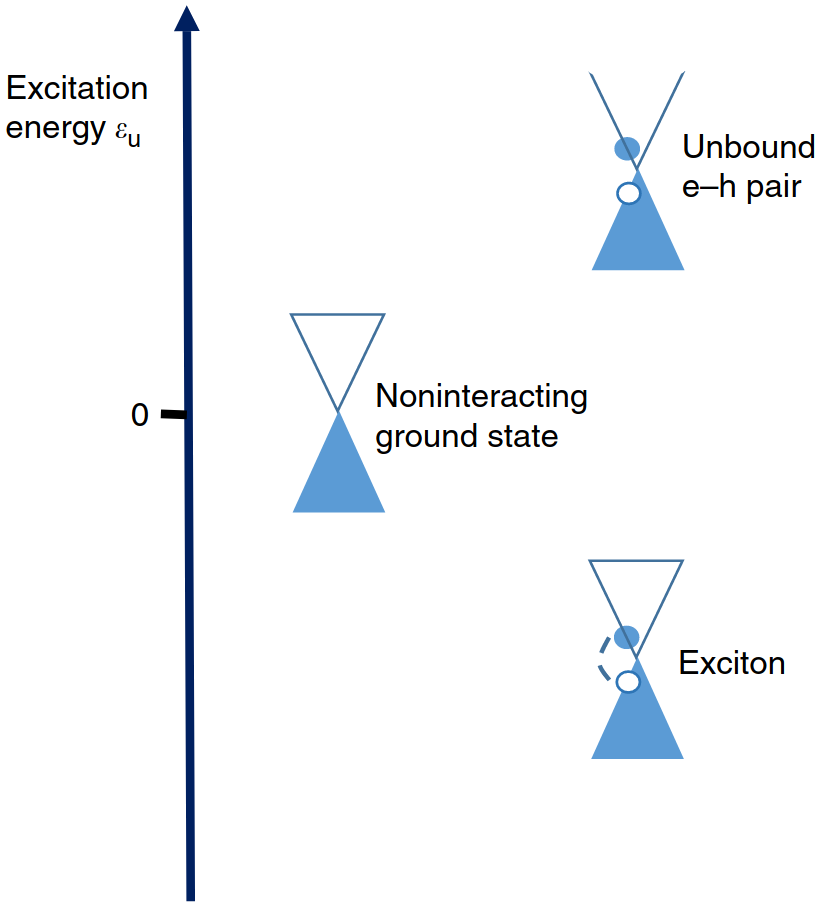
\includegraphics[width=0.35\linewidth]{exciton_gap.png}}
    % \centerline{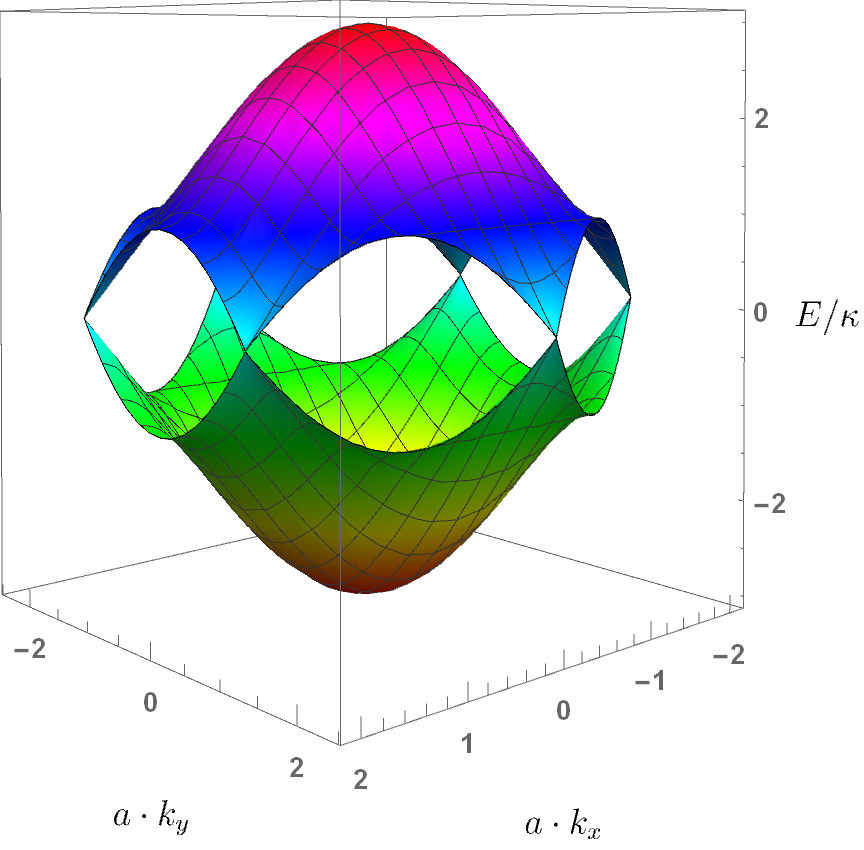
\includegraphics[width=0.7\linewidth]{band_structure.png}}
    \caption{Excitonic instability in carbon nanotubes. The scheme represents the excitation energy $\epsilon_u$ of an electron-hole (e-h) pair relative to the noninteracting ground state, a zero-gap semiconductor. In the absence of interaction, the excitation energy $\epsilon_u$ of an e-h pair is positive. The long-range interaction may bind e-h pairs close to the Dirac point in the momentum space. If an exciton forms, then its excitation energy $\epsilon_u$ is negative. This instability leads to the reconstruction of the ground state into an excitonic insulator. [CARBON NANO TUBES (took the caption word-for-word)]}
    \label{fig:exciton_gap}
\end{figure}

% Developments
In recent years, there has been a renewed interest in investigating excitons due to their theoretically proposed applications in technology. These excitonic bound states are considered to be good candidates for the development of topologically protected qubits, switching devices, and in heat exchangers [THIN-FILM TOPOLOGICAL INSULATORS(conclusion)]. The properties of the exciton have been studied on a microscopic level by employing Hubbard-like Hamiltonians on graphene lattices as well as the 3D thin-films topological insulators. There are other models (e.g. Gross-Neveu models) that have been used to describe excitons in semimetals and in semiconductors by studying the phase transitions between them and excitonic insulator. It has been shown that the dynamics of the bound electron-hole pair can be controlled in van der Waals heterostructures via a change of twist angle between the monolayers. These properties (most importantly the lifetimes of the excitons) can be tuned from the appearance of moiré potential, which in momentum space translates to relative rotation of both layer's Brillouin zones [TWIST ANGLE HETEROSTRUCTURES].
% Simulations
% On the lattice?
% Different models for excitons

In this work, we apply the Hubbard model onto a hexagonal lattice which is a model of graphene (see Section LATTICE). We are looking for the appearance of an electron-hole bound state. This will be done by measuring the binding energy of the correlation functions ratio
\begin{equation}
    \epsilon = (E_e + E_h) - E_{e-h} = \ln\left( \frac{C_e(\tau)C_h(\tau)}{C_{e-h}(\tau)} \right)
\end{equation}
The Hubbard model that we are applying there is not a mechanism for decay of the exciton state. This means that if the energy is negative ($\epsilon < 0$), we have a bound exciton state; and if the energy is higher than the energy threshold, then the particles are unbound. The study of a monolayer graphene sheets that we do in this thesis is a first step in the direction of future investigation of more complex graphene (and other) structures.

\section{The Hubbard Model}

% Maybe history
The Hubbard model (HM) emerges as a simple solution to the many-body problem in solids. It is a theory that describes the interactions of fermions on lattices, where they can hop between neighboring sites. This model successfully describes the ferromagnetic properties of materials with different strength correlations between electrons. % look-up if true and what to add as citation

% Original Hubbard model Hamiltonian (Tight-binding, interaction, Chemical potential)
The tight-binding with on-site interaction Hamiltonian describes the hopping of the fermions between neighboring sites and the interaction of fermions
\begin{equation}
    H = - \sum_{xy} \left( a^\dagger_{x,\uparrow} K_{xy} a_{y,\uparrow} + a^\dagger_{x,\downarrow} K_{xy} a_{y,\downarrow} \right) - \frac{1}{2} \sum_{x,y} \left( (n^\dagger_{x,\uparrow} - n^\dagger_{x,\downarrow}) V_{xy} (n^\dagger_{y,\uparrow} - n^\dagger_{y,\downarrow}) \right)
\end{equation}
where the first term is the kinetic and the second is the interaction; $a^\dagger$, $a$ are the creation and annihilation operators respectively of electrons, $\uparrow$ is indicating spin-up and $\downarrow$ is spin-down, $K$ is called the hopping matrix which describes the hopping between sites, the interaction term is represented by the potential $V$, and $n_{x,s} = a^\dagger_{x,s} a_{x,s}$ is the electron number density operator. We can make a change of basis, such that particles are separated by spin and charge, which we call a particle-hole symmetry (see Section \ref{ssec:ph-trafo})
\begin{equation}
    \begin{aligned}
        p^\dagger_x & \equiv a^\dagger_{x,\uparrow} \qquad\qquad h^\dagger_x & \equiv a_{x,\downarrow} \\
        p_x & \equiv a_{x,\uparrow} \qquad\qquad h_x & \equiv a^\dagger_{x,\downarrow}
    \end{aligned}
    \label{eq:ph-switch}
\end{equation}
where $p^\dagger (p)$, $h^\dagger (h)$ are the creation(annihilation) operators of particles and holes. Since these operators describe fermions, they respect the anti-commutation relations i.e. the Pauli exclusion principle

\begin{equation}
    \begin{aligned}
        \{ p^\dagger_x, p_y \} &= \delta_{xy} &\{ h^\dagger_x, h_y \} = \delta_{xy}
        \\
        \{ p_x, p_y \} &= \{ p^\dagger_x, p^\dagger_y \} = 0 &\{ h_x, h_y \} = \{ h^\dagger_x, h^\dagger_y \} = 0
        \\
        \{ p^\dagger_x, p_y \} &= \{ p^\dagger_x, h^\dagger_y \} = 0 \qquad\qquad &\{ p_x, h_y \} = \{ p_x, h^\dagger_y \} = 0
        \\
    \end{aligned}
\end{equation}
% Particle-hole basis (Creation and annihilation operators)
The convention for spin and charge that we use for the particles and holes operators is given in Table \ref{tab:convention_operators}.
\begin{table}[h]
    \centering
    \begin{tabular}{c|ccc}
        & $Q$ & $S$ & $S^3$ \\
    \hline
        $p^\dagger$ & +1 & $\frac{1}{2}$ & $-\frac{1}{2}$ \\
        $p$ & -1 & $\frac{1}{2}$ & $+\frac{1}{2}$ \\
        $h^\dagger$ & -1 & $\frac{1}{2}$ & $-\frac{1}{2}$ \\
        $h$ & +1 & $\frac{1}{2}$ & $+\frac{1}{2}$ \\
    \end{tabular}
    \caption{Convention of charge ($Q$), spin ($S$), and third component of spin ($S^3$) used for creation and annihilation operators of particles and holes.}
    \label{tab:convention_operators}
\end{table}
Here $Q$, $S$, $S^3$ are the charge, spin, and the third component of the spin respectively. For the two-body correlators (discussed in Section \ref{sec:corr_func}), it is also convenient to know the quantum numbers for different combinations of particle and hole operators. In Table \ref{tab:ph-comb} is given a summary which will be useful in the next chapters. We notice that only the charge and $S^3$ are present in the table. This is due to $Q$ and $S^3$ being additive numbers, whereas the spin is not because two different spin values could have the same third component (ex. $S=0,1;S^3=0$).
\begin{table}[h]
    \centering
    \begin{tabular}{c|cc}
        & $Q$ & $S^3$ \\
    \hline
        $p^\dagger p^\dagger$ & +2 & $-1$ \\
        $p^\dagger p$ & 0 & $0$ \\
        $p^\dagger h^\dagger$ & 0 & $-1$ \\
        $p^\dagger h$ & +2 & $0$ \\
        $p p$ & -2 & $+1$ \\
        $p h^\dagger$ & -2 & $0$ \\
        $p h$ & 0 & $+1$ \\
        $h^\dagger h^\dagger$ & -2 & $-1$ \\
        $h^\dagger h$ & 0 & $0$ \\
        $h h$ & +2 & $+1$ \\
    \end{tabular}
    \caption{Quantum numbers for the combination of particle and hole operators.}
    \label{tab:ph-comb}
\end{table}

% Particle-hole Hubbard Hamiltonian
We can now substitute the operators inside the Hamiltonian with the ones in the new basis
\begin{equation}
    H = - \sum_{xy} \left( p^\dagger_x K_{xy} p_y - h^\dagger_x K_{xy} h_y \right) + \frac{1}{2} \sum_{x,y} \left( (n^\dagger_{x,p} - n^\dagger_{x,h}) V_{xy} (n^\dagger_{y,p} - n^\dagger_{y,h}) \right),
\end{equation}
here we have added a new index to the number density operators which indicates whether particles or holes are counted.

Finally, we can expand our Hamiltonian with one more term, which is called the chemical potential term, where $\mu$ is the chemical potential. It accounts for the change of the number of particles and holes
\begin{equation}
    H - \vec{\mu}\cdot\vec{q} = - \sum_{xy} \left( p^\dagger_x K_{xy} p_y + h^\dagger_x K_{xy} h_y \right) + \frac{1}{2}\sum_{xy} q_x V_{xy} q_y - \sum_{x} \mu_x q_x
\end{equation}
and we have introduced one more operator $q_x = n_{x,p} - n_{x,h}$. This is the charge operator that indicates the relative charge on each site. 

The Hamiltonian of this model for our ease can be divided into two parts -- the half-filling part of the whole Hamiltonian and the chemical potential part. The former contains the kinetic and the interaction terms, whereas the latter in made out of only the chemical term. In the case of bipartite lattices (Chapter "SYMMETRY"), we must be able to differentiate on which lattice sites the operators are. This could be done by modifying the transformation (\ref{eq:ph-switch}) to include site dependent sign $\sigma_k$ for holes
\begin{equation}
    H - \vec{\mu}\cdot\vec{q} = - \sum_{xy} \left( p^\dagger_x K_{xy} p_y + \sigma_k h^\dagger_x K_{xy} h_y \right) + \frac{1}{2}\sum_{xy} q_x V_{xy} q_y - \sum_{x} \mu_x q_x.
\end{equation}

To get to the Hamiltonian that we work with, we choose to have only contact interactions ($V_{xy} = U\delta_{xy}$). This means that the interactions are done only in the same site
\begin{equation}
    H - \vec{\mu}\cdot\vec{q} = - \sum_{xy} \left( p^\dagger_x K_{xy} p_y + \sigma_k h^\dagger_x K_{xy} h_y \right) + \frac{U}{2}\sum_{xy} q^2_x - \sum_{x} \mu_x q_x.
\end{equation}
In this thesis work we sometimes work with the chemical potential, and sometimes we set $\mu = 0$, depending on the symmetries that we use \cite{avoiding ergodicity}. On Figure \ref{fig:hub_scheme} is shown a schematic of the Hubbard model's hopping and interaction.
\begin{figure}[h]
    \begin{center}
        \begin{tikzpicture}
            \tikzstyle{arrow} = [very thick,->,>=stealth]
            \def \spacing{2}
            \draw[step=\spacing,gray,very thin,dashed] (-0.5,-0.5) grid (6.5,6.5);

            \fill[color=black] (0*\spacing,1*\spacing) circle (0.15);
            \draw[color=black] (1*\spacing,1*\spacing) circle (0.15);
            \fill[color=white] (1*\spacing,1*\spacing) circle (0.15);
            \fill[color=black] (2*\spacing,2*\spacing) circle (0.15);
            \draw[color=black] (2*\spacing,3*\spacing) circle (0.15);
            \fill[color=white] (2*\spacing,3*\spacing) circle (0.15);
            \fill[color=black] (1.05*\spacing,2.05*\spacing) circle (0.15) node[anchor=south east] {\textbf{$V$}};
            \draw[color=black] (0.95*\spacing,1.95*\spacing) circle (0.15);
            \fill[color=white] (0.95*\spacing,1.95*\spacing) circle (0.15);
            \draw[color=black] (3*\spacing,1*\spacing) circle (0.15);
            \fill[color=white] (3*\spacing,1*\spacing) circle (0.15);
            \fill[color=black] (0*\spacing,3*\spacing) circle (0.15);
            \draw[color=black] (1.95*\spacing,-0.05*\spacing) circle (0.15);
            \fill[color=white] (1.95*\spacing,-0.05*\spacing) circle (0.15);
            \fill[color=black] (2.05*\spacing,0.05*\spacing) circle (0.15) node[anchor=south east] {\textbf{$V$}};
 
            \draw[arrow, shorten >=5pt, shorten <=5pt] (0*\spacing,1*\spacing) to [bend left=30] node [midway, sloped, above] {$K$} (1*\spacing,1*\spacing);
            \draw[arrow, shorten >=5pt, shorten <=5pt] (2*\spacing,3*\spacing) to [bend left=30] node [midway, right] {$K$} (2*\spacing,2*\spacing);
        \end{tikzpicture}
        \caption{Schematic view of the hopping and the interaction of electrons with different spin on a square lattice. Here $K$ is the hopping matrix containing the hopping probabilities and $V$ is the interaction potential. In the particle-hole basis the black and white dots represent particles and holes.}
        \label{fig:hub_scheme}
    \end{center}
\end{figure}
% Problems
The theory that we are working with as mentioned before is a model of the real physical systems. Even though the HM gives us good results, one must know some drawbacks of the model. One is that it neglects the long range part of the Coulomb forces. It is likely that significant effects are missed by this simplification [MOTT]. Another weakness of this model it has difficulties being applied to transition metals. And the Hubbard model cannot be exactly solved, so approximations must be used.

Despite having these issues, the two-dimensional HM has showed promising results when applied to honeycomb lattices. The description of the electronic structure when applied resembles that of the carbon nano structures, such as graphene, carbon nano tubes, and ribbons.
% Examples of Hubbard model
% Solutions to the model (Exact, not so exact)

% The next part should be tested more
An exact solution to the Hubbard model Hamiltonian exists in the non-interacting case at half filling. Even though, the data and analysis are done with the full Hamiltonian, it is always helpful to know the behavior of the model in the non-interacting case. The pattern that emerges is usually kept in the interacting case, and this will give us something to compare to. Since we are applying HM on the hexagonal lattice (see section LATTICE) in this work, we have the following two-band dispersion relation
\begin{equation}
    E_{\vec{k}\pm} = \pm (-\kappa) \sqrt{3 + 2 \left( \cos\left( \frac{3}{2}k_x + \frac{\sqrt{3}}{2}k_y \right) + \cos\left( \frac{3}{2}k_x - \frac{\sqrt{3}}{2}k_y \right) + \cos\left( \sqrt{3}k_y \right) \right)},
\end{equation}
where $k$ is the momentum mode and $\kappa$ is the hopping parameter. In Figure \ref{fig:two-band}, it is shown how the exact solution of the band structure looks like for infinite and finite volume lattices. One notices that for infinite lattice volume the momentum modes are continuously filled, and the model gets the full symmetry of the lattice. Whereas in the finite volume regime only a finite number of momentum modes are available to us. The symmetry is also kept in the finite volume regime with lattices that have $L_1 = L_2$; and for every other configuration of hexagonal lattice, the full symmetry is broken to other symmetries. We expect to keep the two-band structure, even if we add the interaction term and chemical potential term. Therefore, we must add a label to the ladder operators indicating the band that they are applied to. For further information on the symmetries of the lattice and the model, see chapter SYMMETRY.
% Creation and annihilation operators convention
\begin{figure}[htbp]
    \centerline{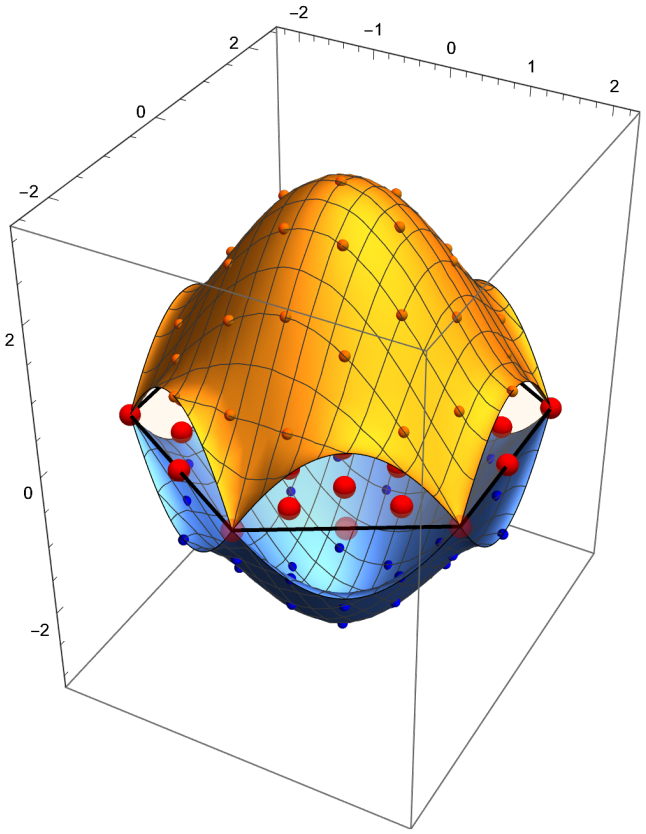
\includegraphics[width=0.5\linewidth]{two-band-structure.png}}
    % \centerline{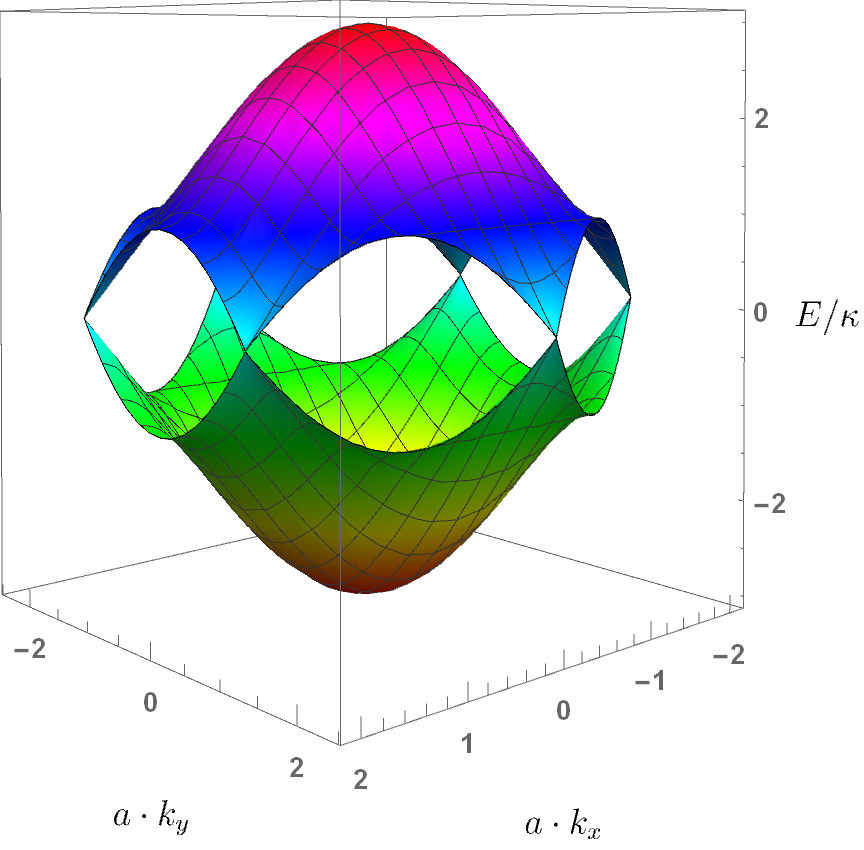
\includegraphics[width=0.7\linewidth]{band_structure.png}}
    \caption{The noninteracting one-body spectrum on the honeycomb lattice. The BZ is shown as a black hexagon, while the red spheres are the momenta allowed on a $L_1 = 6$, $L_2 = 6$ lattice and the orange and blue spheres are the corresponding non-interacting energies. [EVAN'S PAPER]}
    \label{fig:two-band}
\end{figure}


\section{Corelation Functions}
\label{sec:corr_func}

The correlation functions (correlators) that we are interested in ($\langle \mathcal{O}_{x,t+\tau}\mathcal{O}^\dagger_{y,t} \rangle$), are called Euclidean correlators. They are defined as a thermal trace
\begin{equation}
    \langle \mathcal{O}_{x,t+\tau}\mathcal{O}_{y,t} \rangle = \frac{1}{\mathcal{Z}}tr\left[ \mathcal{O}_{x,t+\tau}\mathcal{O}_{y,t}\mathrm{e}^{-\beta H} \right],
\end{equation}
where the $\mathcal{O}$ operators could be operators that create or annihilate states (usually the adjoint operator creates the anti-state), measure observables, or a combination of these; the labels $x$ and $y$ are there to indicate any set of labels, not just a position, $\mathcal{Z} = tr\left[ \mathrm{e}^{-\beta H} \right]$ is the partition function, $\beta$ is the inverse temperature, and $H$ is a general Hamiltonian of a model. In our case model, the field operators create states with a set of quantum numbers that define it at some time $t$ and destroy the same states at a different time $t + \tau$. These operators can also be composite $\mathcal{O} = \mathcal{O'}_1\mathcal{O'}_2\hdots\mathcal{O'}_n$. We can make a time transformation (assuming the action is time-translation invariant), such that the source is at time zero and the sink is at time $\tau$. Then, we move to the Heisenberg picture, so the correlator becomes
\begin{equation}
    C_{xy}(\tau) := \langle \mathcal{O}_{x,\tau}\mathcal{O}_{y,0} \rangle = \frac{1}{\mathcal{Z}}tr\left[ \mathcal{O}_{x,\tau}\mathrm{e}^{-H\tau}\mathcal{O}_{y,0}\mathrm{e}^{-H(\beta - \tau)} \right]
\end{equation}
We drop the time labels that are on the operators, since we work with the Hubbard model, and we can always make the time translation that we have discussed.

In order to be able to extract energies from the correlators, we must first find the spectral decomposition. This could be done by inserting the identity operator $\mathds{1}$ written in terms of complete set of orthonormal basis
\begin{equation}
    \mathds{1} = \sum_\alpha | n \rangle \langle n |
\end{equation}
in between the operators of the expanded in the eigenbasis of the Hamiltonian thermal trace
\begin{equation}
    \begin{aligned}
        C_{xy}(\tau) &= \frac{1}{\mathcal{Z}}tr\left[ \mathcal{O}_x\mathrm{e}^{-H\tau}\mathcal{O}_y\mathrm{e}^{-H(\beta - \tau)} \right] 
        \\
        &= \frac{1}{\mathcal{Z}}\sum_\alpha\langle \alpha | \mathcal{O}_x\mathrm{e}^{-H\tau}\mathcal{O}_y\mathrm{e}^{-H(\beta - \tau)} | \alpha \rangle 
        \\
        &= \frac{1}{\mathcal{Z}}\sum_{\alpha mnl} \langle \alpha | \mathcal{O}_x | m \rangle \langle m | \mathrm{e}^{-H\tau} | n \rangle \langle n | \mathcal{O}_y | l \rangle \langle l | \mathrm{e}^{-H(\beta - \tau)} | \alpha \rangle 
        \\
        &= \frac{1}{\mathcal{Z}}\sum_{\alpha mnl}\langle \alpha | \mathcal{O}_x | m \rangle \delta_{mn}\mathrm{e}^{-E_n\tau} \langle n | \mathcal{O}_y | l \rangle \delta_{l\alpha}\mathrm{e}^{-E_\alpha(\beta - \tau)}
        \\
        &= \frac{1}{\mathcal{Z}}\sum_{\alpha n}\langle \alpha | \mathcal{O}_x | n \rangle \langle n | \mathcal{O}_y | \alpha \rangle \mathrm{e}^{-E_n\tau} \mathrm{e}^{-E_\alpha(\beta - \tau)}
        \\
        &= \frac{1}{\mathcal{Z}}\sum_{\alpha n} \mathfrak{u}_{\alpha xn} \mathfrak{u}_{ ny\alpha} \mathrm{e}^{-E_n\tau} \mathrm{e}^{-E_\alpha(\beta - \tau)},
        \\
    \end{aligned}
    \label{eq:fit_exponent}
\end{equation}
where $\mathfrak{u}_{\alpha xn}$ and $\mathfrak{u}_{ ny\alpha}$ are the overlap factors. In the limit $\beta \to \infty$, one of the exponents vanishes, meaning the lowest excited state dominates
\begin{equation}
    \lim_{\beta \to \infty} C_{xy}(\tau) = \sum_{n} \mathfrak{u}_{\Omega xn} \mathfrak{u}_{ ny\Omega} \mathrm{e}^{-\Delta E_n\tau}
    \label{eq:beta_lim}
\end{equation}
where $\Delta E_n = E_n - E_\Omega$, and $\Omega$ denotes the lowest energy state (vacuum state).

Another way to express the two-point correlator is by using a Euclidean path integral
\begin{equation}
    C_{xy}(\tau) = \langle \mathcal{O}_x\mathcal{O}^\dagger_y \rangle = \frac{1}{\mathcal{Z}} \int \mathcal{D}\phi \:\mathrm{e}^{-S[\phi]}\times \left(\mathcal{O}_x\mathcal{O}^\dagger_y\right)_{Wick},
    \label{eq:path-int}
\end{equation}
where $\mathcal{D}\phi$ is the path integral measure, $S[\phi]$ is the Euclidean action, $\mathcal{Z}$ is the partition function defined as
\begin{equation}
    \mathcal{Z} = \int \mathcal{D}\phi \:\mathrm{e}^{-S[\phi]};
\end{equation}
the label $Wick$ indicates that all possible Wick contractions must be performed on the operators, where each term is a product of inverse fermion matrices ($M^{-1}$) [GATRINGER WICK'S THEOREM]. As this is very important to the part where we generate data, we will explicitly work out two examples -- one for a one-body correlation function and the other for a two-body correlator with two Wick contractions.

\begin{itemize}
    \item \textbf{One-body correlation function}\\
    We start by substituting the general operator $\mathcal{O}$ with the particle ladder operator $p$ and their adjoints. Then, we construct the correlation function and use Wick's theorem to perform the contractions
    \begin{equation}
        \begin{aligned}
            \langle p_{x}p^\dagger_{y} \rangle &= \frac{1}{\mathcal{Z}} \int \mathcal{D}\phi \:\mathrm{e}^{-S[\phi]}\times \left(p_{x}p^\dagger_{y}\right)_{Wick} 
            \\
            &= \frac{1}{\mathcal{Z}} \int \mathcal{D}\phi \:\mathrm{e}^{-S[\phi]} M[\phi]^{-1}_{(x,y)},
        \end{aligned}
    \end{equation}
    where $x$,$y$ denote the position of the particle and $M[\phi]$ is the fermion matrix. The same derivation can be performed for $\langle h_xh^\dagger_y\rangle$.
    
    \item \textbf{Two-body correlation function}\\
    In this example, we want to show what the Wick contractions are for composite operators. We start again by substituting the general operators from \ref{eq:path-int} with $pp$ and the adjoint. Then, we expand the $\left(\dots\right)_{Wick}$, and finally we substitute $M[\phi]^{-1}$ in each term
    \begin{equation}
        \begin{aligned}
            \langle p_{1,x}p_{2,x'}p^\dagger_{3,y}p^\dagger_{4,y'} \rangle &= \frac{1}{\mathcal{Z}} \int \mathcal{D}\phi \:\mathrm{e}^{-S[\phi]}\times \left(p_{1,x}p_{2,x'}p^\dagger_{3,y}p^\dagger_{4,y'}\right)_{Wick} 
            \\
            &= \frac{1}{\mathcal{Z}} \int \mathcal{D}\phi \:\mathrm{e}^{-S[\phi]}\times \left(\wick{\c1 p_{1,x} \c2 p_{2,x'} \c2 p^\dagger_{3,y} \c1 p^\dagger_{4,y'} - \c3 p_{1,x} \c4 p_{2,x'} \c3 p^\dagger_{3,y} \c4 p^\dagger_{4,y'}}\right)_{Wick} 
            \\
            &= \frac{1}{\mathcal{Z}} \int \mathcal{D}\phi \:\mathrm{e}^{-S[\phi]} \left((M[\phi]^{-1}_{14})_{(x,y')}(M[\phi]^{-1}_{23})_{(x',y)} - (M[\phi]^{-1}_{13})_{(x,y)}(M[\phi]^{-1}_{24})_{(x',y')}\right)
        \end{aligned}
    \end{equation}
    where the number labels indicate which operators are replaced with the fermion propagator; the relative minus sign between the terms is due to the odd permutation.
\end{itemize}

The representation of the correlation functions as path integral is as mentioned important to us because we have a way to generate the correlation functions. This can be done by numerically solving the integrals using stochastic methods (SECTION HMC) for Gausian integration. Then, it is possible to extract the energies of the correlators if we fit \ref{eq:fit_exponent} for different $\beta$ and volumes, and, finally, extrapolate to zero temperature (\ref{eq:beta_lim}) and infinite volume. This will give us the result we are looking for.

% One particle gap

% Fermionic matrix (Path integral, Inversion)
% Two particle gap
% Exponential representation of the correlator
% Effective mass
% Binding energy

% !TEX root = mythesis.tex

%==============================================================================
\chapter{Methods}
\label{sec:methods}
%==============================================================================
% History
% Pros & Cons
% Ergodisity (Avoiding problems)
% Application of HMC onto the lattice
% Bootstrap
\section{Hybrid Monte Carlo}
% MCMC
%% Why these algos are better that a MC
%% Markov chain definition
%%% Stationary distribution
%%% Detailed balance
% Hamiltonian Dynamics
%% Leapfrog integrator
% Metropolis Hastings
% Summary of the algo
The Hybrid (Hamiltonian) Monte Carlo (HMC) algorithm is the workhorse of modern Lattice QCD simulations and other Hamiltonian theories~\cite{hmccm}. This is due to the difficulty of simulating fermions with their anti-commuting nature using standard Monte Carlo (MC) methods. The major advantage of HMC over other methods is that this algorithm updates the system globally instead of the local updates that standard MC methods use. Moreover, the method is exact, meaning it does not have and truncation errors and the ensemble averages do not depend on the integration step size. These two advantages reduce the critical slowing down from which the other MC methods suffer. In the following subsections we will discuss in some detail the individual methods and algorithms that are involved in the creation of HMC.

\subsection{Markov Chain Monte Carlo}

Monte Carlo algorithms in general are used in quantum field theory to calculate the expectation value of an observable, leveraging the law of large numbers

\begin{equation}
    \langle\mathcal{O}\rangle = \frac{1}{Z} \int d\phi \mathcal{O} e^{-S[\phi]},
\end{equation}
where
\begin{equation}
    Z = \int d\phi e^{-S[\phi]}
\end{equation}
This is done by sampling $\phi$ fields from a distribution
\begin{equation}
    P(\phi) = \frac{1}{Z} \int d\phi e^{-S[\phi]}
\end{equation}
and then calculating the average
\begin{equation}
    \overline{\mathcal{O}} \equiv \frac{1}{N}\sum^{N}_{n=1} \mathcal{O}(\phi_n)
    \label{eq:ensamble_average}
\end{equation}
And in the limit of $N \to \infty$, we get the relation
\begin{equation}
    \overline{\mathcal{O}} = \langle\mathcal{O}\rangle + \mathrm{O}(1/\sqrt{N})
\end{equation}

Making simulations by sampling directly from distributions could prove very costly and practically impossible. This is because the phase space of the target distribution might be too big to explore it all (curse of dimensionality). A much better way to explore the phase space is by progressively uncovering the regions of interest~\cite{mhexpl}, which could be done by the use of Markov Chain.

The Markov Chain~\cite{intromarkov} is defined as a sequence of random variables $X_n$, where every next element is generated from the previous element in the chain by a transition matrix $P_{ii+1}$
\begin{equation}
    X_0 \xrightarrow{P_{01}} X_1 \xrightarrow{P_{12}} X_2 \xrightarrow{P_{23}} \cdots \xrightarrow{P_{n-1n}} X_n
\end{equation}
If the chain is ergodic and positive recurrent, then the detailed balance condition ensures that the Markov chain converges to a unique stationary distribution $p$
\begin{equation}
    p(X_i) P_{ij} = p(X_j) P_{ji}
\end{equation}

All Monte Carlo algorithm that use this method of random variable sampling are called Markov Chain Monte Carlo (MCMC) algorithms. HMC is a MCMC algorithm since we use a Markov chain to explore the target distribution, from which we draw the $\phi$ fields.

\subsection{Hamilton Dynamics}

The proposed updates to the system that we work with, must not change the energy. This is exactly what the Hamilton dynamics do. They preserve the Hamiltonian (the energy of the system). Therefore, we define Hamiltonian dynamics to evolve our $\phi(\tau)$, where $\tau$ is an evolution parameter~\cite{hmc}. We introduce conjugate momenta $\pi(\tau)$ and a Hamiltonian 
\begin{equation}
    H(\phi,\pi) \equiv \frac{1}{2}\pi^2 + S(\phi),
\end{equation}
where $S(\phi)$ is the action. Now, can use the equations of motion to evolve $\phi$
\begin{equation}
    \dot{\phi} = \frac{\delta H}{\delta \pi} \qquad \dot{\pi} = - \frac{\delta H}{\delta \phi} = - \frac{\delta S}{\delta \phi}
    \label{eq:eom}
\end{equation}
The initial momentum $\pi$ is selected from a Gaussian distribution function with mean zero and unit variance. Then the whole system is evolved though the ($\phi,\pi$)-phase space. There are a lot of algorithms that can be used to solve (\ref{eq:eom}) but the most common method is the Leapfrog integrator. It is reversible and preserves the area which makes it a perfect candidate, due to the detailed balance requirement. The algorithm is simple; with initial half-step
\begin{equation}
    \pi\left(\frac{\delta\tau}{2}\right) = \pi\left(0\right) - \left[ \frac{\delta S(0)}{\delta\phi} \right] \frac{\delta\tau}{2}
\end{equation}
This is followed by $n=\frac{\tau_0}{\delta\tau}$ steps in $\phi$ and $n-1$ in $\pi$
\begin{equation}
    \begin{aligned}
        \phi(\tau+\delta\tau) = \phi(\tau) + \pi(\tau+\frac{\delta\tau}{2})\delta\tau
        \\
        \pi(\tau+\frac{\delta\tau}{2}) = \pi(\tau-\frac{\delta\tau}{2}) - \left[ \frac{\delta S(\tau)}{\delta\phi} \right] \delta\tau
    \end{aligned}
\end{equation}
and again half-step in $\pi$
\begin{equation}
    \pi(\tau_0) = \pi(\tau_0-\frac{\delta\tau}{2}) - \left[ \frac{\delta S(\tau_0)}{\delta\phi} \right] \frac{\delta\tau}{2}
\end{equation}
On Figure \ref{fig:leapfrog} is show a schematic view of the leapfrog integration process.
\begin{figure}[htbp]
    \centerline{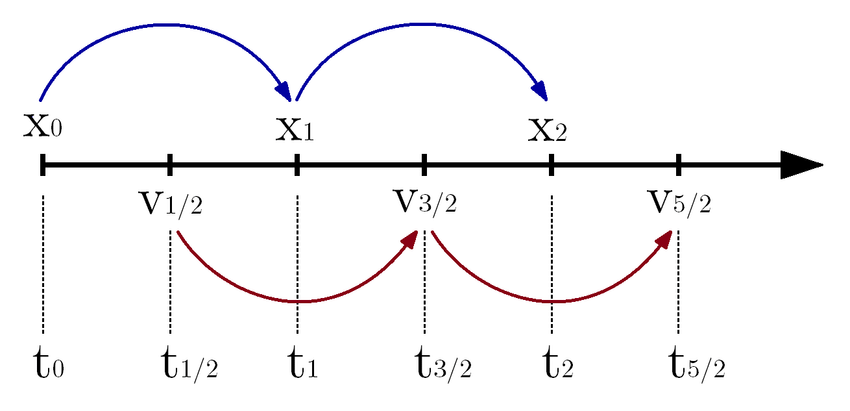
\includegraphics[width=0.5\linewidth]{leapfrog.png}}
    \caption{Leapfrog integration process. The scheme represents one integration trajectory. On each step of evolution, one of the variables lead the other by a half step, and they update each other. %https://www.researchgate.net/figure/Schematics-describing-how-the-leapfrog-algorithm-works-Position-and-velocity-leap-each_fig1_346972792}
    }
    \label{fig:leapfrog}
\end{figure}

\subsection{Metropolis-Hastings}

A Metropolis-Hastings accept/reject algorithm~\cite{mhog, mhexpl} is used to construct a Markov chain with a stationary distribution $p(X)$. This is done by having a candidate element with transition probability $P_{acc}$. The accepted proposal is the new element of the chain, but if it is rejected the old element becomes the new one. This algorithm preserves the stationary distribution if the chain is irreducible.

\begin{figure}[htbp]
    \centerline{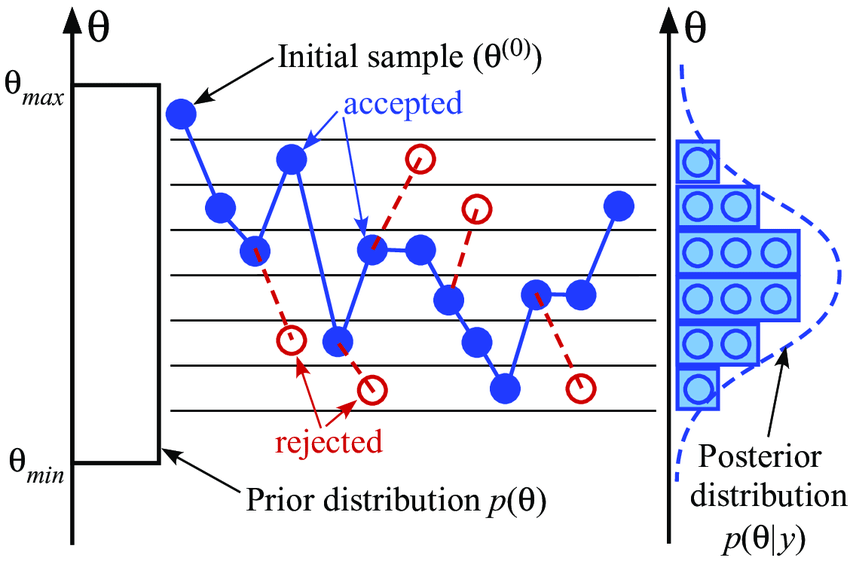
\includegraphics[width=0.5\linewidth]{
        Metropolis-Hastings-MCMC.png}}
    \caption{Metropolis-Hastings process for generating a Markov chain with a target distribution. The scheme represents the transition from an initial probability distribution to a target one. On each step, the accept/reject step is performed on the candidate element. The first element of the Markov chain is drawn from the starting distribution. The whole process is repeated until all sampled elements are representative of the new distribution. %https://www.researchgate.net/figure/Illustration-of-the-Markov-chain-Monte-Carlo-with-Metropolis-Hastings-MCMC-MH-procedure_fig6_338363810
    }
    \label{fig:mn-mcmc}
\end{figure}
This algorithm is used in HMC as an accept/reject step on the new proposed $\phi$ field. The candidate is accepted with probability 
\begin{equation}
    P_{acc} = min(1, \exp(\delta H)),
\end{equation}
where $\delta H = H' - H$ is the difference of the final and the starting Hamiltonians. This difference $\delta H$ is not zero because of the finite number of integration steps. The whole process repeats until we are satisfied by the number of configuration in the constructed Markov chain which will be averaged in (\ref{eq:ensamble_average}). On Figure \ref{fig:mn-mcmc} is shown how the Markov chain is constructed using the Metropolis-Hastings accept/reject algorithm. This acceptance rate can be tuned by the number of integration steps which can make the exploration of the phase space easier.

\subsection{Summary of the Algorithm}

We have discussed until now how we compute numerically the expectation value (\ref{eq:ensamble_average}) of an observable using MC algorithms. We also saw a better approach to draw from distributions that are difficult to sample using MCMC methods. This approach uses proposed elements which construct a Markov chain. These candidates can be found by leveraging the Hamilton dynamics and can be accepted with a probability $P_{acc}$. All of these methods culminate in the HMC algorithm~\cite{hmc}, which is summarized in Algorithm (\ref{alg:hmc})

\begin{algorithm}
    \caption{Hybrid Monte Carlo}
    \begin{algorithmic}[1]
        \State Initialize  $\tau, N_{max}$
        \State Initialize $\phi_0, \pi_0$
        \State Sample $\pi_0 \sim \mathcal{N}(0,1)$

        \State Set $(\phi_{i}, \pi_{i}) = (\phi_0, \pi'_0)$ \Comment{Initial Condition}
        \While{$i < N_{max}$}  \Comment{Markov Chain}
            \State Calculate $H(\phi_{i}, \pi_{i})$
            \State Leapfrog $(\phi', \pi') \xleftarrow{\tau_\text{steps}} (\phi_{i}, \pi_{i})$ \Comment{Find a candidate}
            \State Calculate $H'(\phi',\pi')$
            \State Calculate $\delta H = H'(\phi',\pi')-H(\phi_{i},\pi_{i})$
            \If{$P_{acc} = min(1, \exp(-\delta H))$} \Comment{Accept/Reject step}
                \State Set $(\phi_{i+1}, \pi_{i+1}) = (\phi', \pi')$
                \Else
                \State Set $(\phi_{i+1}, \pi_{i+1}) = (\phi_{i}, \pi_{i})$
            \EndIf
        \State Set $i = i + 1$
        \EndWhile
    \end{algorithmic}
    \label{alg:hmc}
    \end{algorithm}

\section{Linear Solvers}

We saw in Section \ref{sec:corr_func} that if we want to numerically compute the expectation value of the correlation functions, we must work with a lot of inverse matrices. Therefore, we must find a method for inverting matrices, which could be either a direct or an iterative method of solving linear systems of equations
\begin{equation}
    Ax = b
    \label{eq:lineq}
\end{equation}
In this work, we use the latter methods, namely the Flexible Generalized Minimum Residual (FGMRES) method~\cite{fgmresart}. This method can be used for any invertible matrix, but it usually converges very slow. Some even make an analogy with a tank, because it is slow but robust and if there is a solution, it will find it. A solution to the speed of the algorithm is to use a preconditioner. We have chosen to use the Conjugate Gradient (CG) method~\cite{cgbook}. In the next subsections, we will discuss how both methods work. This includes the application of CG as a preconditioner to FGMRES.

\subsection{Conjugate Gradient}

Conjugate gradient is used as an iterative method of solving linear systems of equations that are too large to solve directly. And more precisely with real,  positive-definite usually with sparse matrices. The idea of the algorithm is to have a number of orthogonal search directions. And each search direction is explored fully before going to the next. This method can be viewed as an improved version of the gradient descent method, where the search is always done in the direction of the gradient. A comparison between the methods is shown on Figure \ref{fig:cg_comp}.
\begin{figure}[htbp]
    \centerline{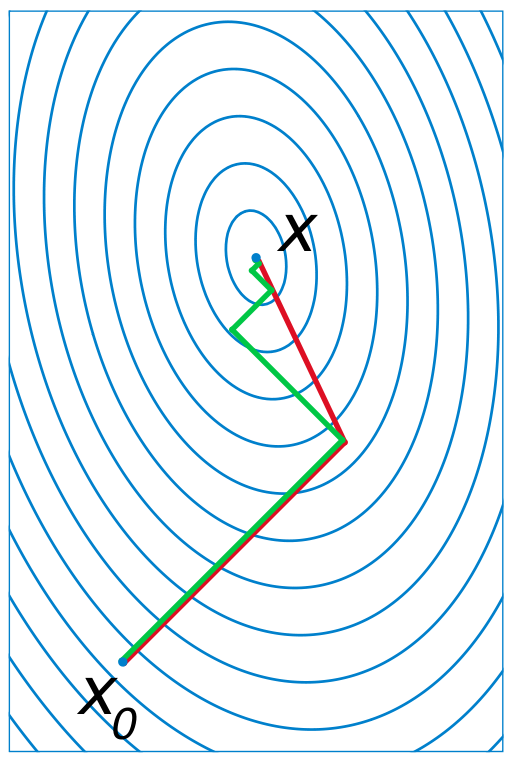
\includegraphics[width=0.5\linewidth]{CG_comparison.png}}
    \caption{Comparison between Conjugate gradient (red) and Gradient descent (green) methods. This is done with the same starting point and an optimal step size for the GD.}
    \label{fig:cg_comp}
\end{figure}

The way we start with the derivation is with the definition of an $A$-matrix inner product for any two vectors
\begin{equation}
    \left( u, v \right)_A = u^\top A v
    \label{eq:cg_constraint}
\end{equation}
and if the product is equal to zero, these vectors are conjugate. Now, we can make a basis of mutually conjugate vectors $\{ p_i \}$, so that we could represent the solution $x'$ of (\ref{eq:lineq}) as a linear combination
\begin{equation}
    x' = \sum_i \alpha_i p_i,
\end{equation}
where
\begin{equation}
    \alpha_i = \frac{\left( p_i, b \right)}{\left( p_i, p_i \right)_A}
\end{equation}

In most cases it is not possible to get the exact result, due to round off error, and one must be content with an approximation of the true result. This means that we do not actually need all conjugate vectors of the basis in order to find a good solution, but we can progressively add more vectors until we are satisfied with the solution.

To show this, we start again with (\ref{eq:lineq}) which is the minimizer (gradient) of a quadratic function
\begin{equation}
    \begin{aligned}
        f(x) &= \frac{1}{2} x^\top A x - x^\top b
        \\
        \nabla f(x) &=  Ax - b
    \end{aligned}
\end{equation}
The goal is to find the minimum, so we define a residual 
\begin{equation}
    r_k = b - Ax_k,
\end{equation}
which measures how close we are to the minimum. And iteratively, the new residual can be computed from the previous
\begin{equation}
    r_{k+1} = r_k - \alpha_k Ap_k,
\end{equation}
where
\begin{equation}
    \alpha_k = \frac{\left( r_k, r_k \right)}{\left( p_k, p_k \right)_A}
\end{equation}
In the Steepest descent method, we use the residuals as search directions, but the improved version that we work with, puts a constraint (\ref{eq:cg_constraint}) on the searches. In order to ensure that the directions are linearly independent, we perform some form of Gram-Schmidt orthogonalization procedure on the residuals where every new $A$-orthogonal vector can be calculated from the previous
\begin{equation}
    p_{k+1} = r_{k+1} + \beta p_k,
\end{equation}
where
\begin{align}
    \beta &= \frac{\left( r_{k+1}, r_{k+1} \right)}{\left( r_k, r_k \right)}
\end{align}
And the new solution can be found by
\begin{equation}
    x_{k+1} = x_k + \alpha_k p_k
\end{equation}
A detailed derivation of CG can be found in~\cite{cgbook}. The whole method can be implemented in an algorithm which can be written in pseudocode (Algorithm \ref{alg:cg}) like

\begin{algorithm}
    \caption{Conjugate Gradient}
    \begin{algorithmic}[1]
        \State Initialize  $A, x_0, b$
        \State Initialize $\epsilon$ \Comment{Convergence criteria}
        \State Set $r_0 = b - Ax_0$ \Comment{Initial Condition}
        \State Set $p_0 = r_0$ \Comment{Initial Search Direction}
        \While{$r_{k+1} > \epsilon$}
            \State Set $\alpha_k = \frac{\left( r_k, r_k \right)}{\left( Ap_k, p_k \right)}$
            \State Update $x_{k+1} = x_k + \alpha_k p_k$
            \State Update $r_{k+1} = r_k - \alpha_k Ap_k$
            \State Set $\beta = \frac{\left( r_{k+1}, r_{k+1} \right)}{\left( r_k, r_k \right)}$
            \State Update $p_{k+1} = r_{k+1} + \beta p_k$
        \EndWhile
    \end{algorithmic}
    \label{alg:cg}
    \end{algorithm}

\subsection{Flexible Generalized Minimum Residual}

This method is a variant of the GMRES method with preconditioning. It is called flexible because it can have different preconditioning on each step of the algorithm, whereas in the previous versions it can have only the same preconditioner on each step. It will be easier to understand the whole FGMRES method if we first explain how the preconditioned GMRES works.

The GMRES algorithm is trying to find an approximate solution to (\ref{eq:lineq}) by building a Krylov subspace, which is defined as
\begin{equation}
    \mathcal{K}_n = \mathcal{K}_n (A, r_0) = span \{ r_0, Ar_0, A^2r_0,\hdots, A^{n-1}r_0 \}
\end{equation}
An important property of this subspace is that the vectors are linearly independent, therefore we can use them as a basis to represent our solution. This is done by applying an Arnoldi method, which can find an orthonormal basis in $\mathcal{K}_n$. The process creates a matrix $\bar{H}_m = H_{(m+1)\times m}$. This matrix is used for minimizing the residual $y_m = min(\beta e_1 - \bar{H}_m y)$, which updates the approximation of the solution $x_m = x_0 + Z_my_m$.

As it was written before, this method is robust but slow. So, in order to improve the speed of convergence, we can precondition the original matrix. In FGMRES, we use the right preconditioning
\begin{equation}
    AM^{-1}(Mx) = b,
\end{equation}
where $M$ is a matrix that can be found very easy with another algorithm by solving $Mz = v$. One could use a lot of different methods for preconditioning. They could be not only one-step methods but also iterative techniques like SSOR, ADI, CG, and even GMRES. The detailed derivation of the method can be found in~\cite{fgmresart}, but here we can only show the general idea of the algorithm with a pseudocode (Algorithm \ref{alg:fgmres})

\begin{algorithm}
    \caption{Flexible Generalized Minimum Residual}
    \begin{algorithmic}[1]
        \State Initialize $\epsilon$ \Comment{Convergence criteria}
        \State Initialize  $A, x_0, b$
        \State Initialize $\bar{H}_m$
        \While{$r_m > \epsilon$}
            \State Compute $r_0 = b - Ax_0$
            \State Set $\beta = ||r_0||$
            \State Compute $v_1 = \frac{r_0}{\beta}$
            \For{$j = 1, 2, ..., m$} \Comment{Arnoldi process}
                \State Compute $z_j = M^{-1}_jv_j$ \Comment{Preconditioning (could be different on every step)}
                \State Compute $w = Az_j$
                \For{$i = 1, ..., j$}
                    \State Compute $h_{i,j} = (w, v_i)$
                    \State Compute $w = w - h_{i,j}v_i$
                \EndFor
                \State Set $h_{j+1,j} = ||w||$
                \State Set $v_{j+1} = \frac{w}{h_{j+1,j}}$
            \EndFor
            \State Set $Z_m = [z_1, ..., z_m]$
            \State Compute $y_m = min(\beta e_1 - \bar{H}_m y)$ \Comment{Least square minimization}
            \State Update $x_m = x_0 + Z_my_m$
            \State Update $r_m = b - Ax_m$
            \State Set $x_0 = x_m$
        \EndWhile
    \end{algorithmic}
    \label{alg:fgmres}
    \end{algorithm}

% !TEX root = mythesis.tex

%==============================================================================
\chapter{Symmetries}
\label{sec:symmetries}
%==============================================================================

A very important aspect of the analysis are the symmetries. They let us extract useful information from the available data. We can leverage the symmetries we have found, so that we can reduce the numerical uncertainties of our data by averaging, or we can reduce the computational cost by declaring two results are the same by symmetry~\cite{evan}. The term means any operation one can perform on an operator that leaves it invariant.

In this chapter we will see what is the symmetry of the lattice, which transformations are symmetry operators of the Hubbard model Hamiltonian, and how they transform the correlation functions that we are interested in. This will help us better our data and the results we extract from it.

\section{Lattice}
\label{sec:lattice}
% Hexagonal lattice (BESTAGONAL :D)

The honeycomb lattice is a 2D lattice where the points of the primitive cell lie on the vertices of a hexagon. The reciprocal lattice is also hexagonal. The honeycomb lattice can be seen as made of two triangular lattices. Lattices with this property are called a bipartite. In general, a bipartite is any lattice which we can make from two overlapping lattices, where every point of one of the sublattices is only neighboring points from the other sublattice~\cite{graphhmc}. One of the triangular sublattices of the honeycomb plane is generated by two non-orthogonal vectors
\begin{equation}
  \vec{a}_1 = \frac{\sqrt{3}}{2}
  \begin{pmatrix}
    \sqrt{3} \\
    +1
  \end{pmatrix} \qquad \qquad
  \vec{a}_2 = \frac{\sqrt{3}}{2}
  \begin{pmatrix}
    \sqrt{3} \\
    -1
  \end{pmatrix}
\end{equation}
By repeating them $L_1$ and $L_2$ times respectively, we can construct the whole finite sublattice. The other one can be constructed simply by offsetting the points with a translation vector $\vec{r} = \pm(\vec{a}_1 + \vec{a}_2)$. On \cref{fig:bipartite} is shown the bipartite of the hexagonal lattice.
\begin{figure}
  \begin{center}
    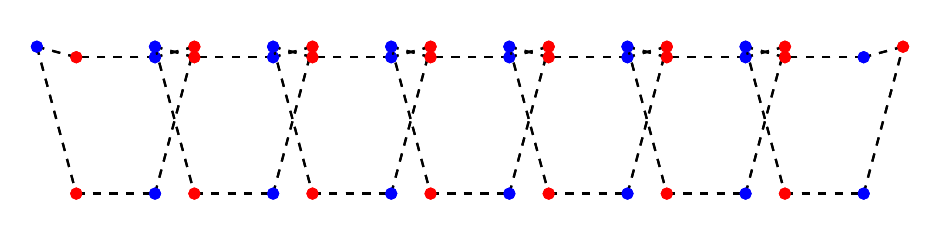
\begin{tikzpicture}
      \foreach \j in {0,1}{
          \foreach \i in {0,1,2,3,4,5,6}{
              \def\spacing{1}
              % the integer division is an implicit floor
              \def\xshift{ \spacing*\i*(3/2) }
              \ifthenelse{\isodd{\i}}{
                  % in plane hexagons
                  \def\yshift{ sqrt(3)*(\j+0.5)*\spacing }
              } {
                  % higher hexagons
                  \def\yshift{ sqrt(3)*\j*\spacing }
              }
              
              \coordinate (A) at ({\xshift+\spacing}         ,{\yshift}                  );
              \coordinate (B) at ({\xshift+\spacing*cos(60)} ,{\yshift+\spacing*sin(60)} );
              \coordinate (C) at ({\xshift+\spacing*cos(120)},{\yshift+\spacing*sin(120)});
              \coordinate (D) at ({\xshift-\spacing}         ,{\yshift}                  );
              \coordinate (E) at ({\xshift+\spacing*cos(240)},{\yshift+\spacing*sin(240)});
              \coordinate (F) at ({\xshift+\spacing*cos(300)},{\yshift+\spacing*sin(300)});

              \draw[thick,dashed,black] (A) -- (B);
              \draw[thick,,dashed,black] (B) -- (C);
              \draw[thick,dashed,black] (C) -- (D);
              \draw[thick,dashed,black] (D) -- (E);
              \draw[thick,dashed,black] (E) -- (F);
              \draw[thick,dashed,black] (F) -- (A);

              \newdimen\r
              \r=2pt
              % Dirac points
              \filldraw[red] (A) circle (\r) node[anchor=north] {};
              \filldraw[blue] (B) circle (\r) node[anchor=south] {};
              \filldraw[red] (C) circle (\r) node[anchor=north] {};
              \filldraw[blue] (D) circle (\r) node[anchor=south] {};
              \filldraw[red] (E) circle (\r) node[anchor=north] {};
              \filldraw[blue] (F) circle (\r) node[anchor=south] {};
          }
      }
    \end{tikzpicture}
    \caption{Honeycomb lattice is a bipartite lattice because we can separate and label the lattice points with different colors (in this example blue and red) in such a way that every point in blue color neighbors only points with red color.}
    \label{fig:bipartite}
  \end{center}
\end{figure}

% Write what the symmetries of the lattice are
In order to investigate the symmetry operators and how they transform the correlation functions, we work with the reciprocal lattice. The primitive cell of the reciprocal is called Brillouin zone (BZ). Some points on the lattice which are of special interest have labels that are used in the literature and in this thesis. These are the center of the first Brillouin zone called the Gamma point ($\Gamma$), the two points on the vertices of the BZ called the Dirac points ($K, K'$), and the three middle of the edges of the BZ points $M, M', M''$. They are all shown on \cref{fig:points} as well as the first neighbors. The graph shows that the first BZ exhibits all the symmetries of the lattice, since the plane wave with a specific mode outside the 1st BZ is exactly equal to a plane wave with a momentum inside the BZ. Therefore, we do not need to investigate beyond it. So, we consider only the first Brillouin zone in our calculations.
\begin{figure}
\begin{center}
  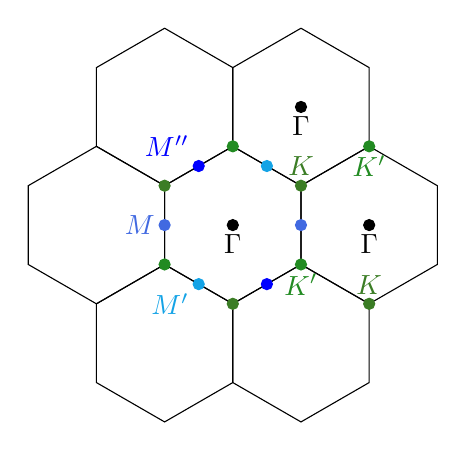
\begin{tikzpicture}
    \newdimen\R
    \R=1cm
    \foreach \x/\y in
      {
        0/0,
        1.732050808/0,
        0.8660254038/1.5,
        -0.8660254038/1.5,
        -1.732050808/0,
        -0.8660254038/-1.5,
        0.8660254038/-1.5
      }
      {
        \begin{scope}[xshift=\x\R, yshift=\y\R]
          \draw (90:\R) \foreach \theta in {150,210,270,330,390,450} { -- (\theta:\R)};
        \end{scope};
      }
    \newdimen\r
    \r=2pt

    % Gamma points
    \filldraw[black] (0,0) circle (\r) node[anchor=north] {$\Gamma$};
    \filldraw[black] (1.732050808\R,0) circle (\r) node[anchor=north] {$\Gamma$};
    \filldraw[black] (0.8660254038\R, 1.5\R) circle (\r) node[anchor=north] {$\Gamma$};

    % Dirac points
    \filldraw[ForestGreen] (-30:\R) circle (\r) node[anchor=north] {$K'$};
    \foreach \theta in {90,210}{\filldraw[ForestGreen] (\theta:\R) circle (\r) ;};
    \filldraw[ForestGreen] (30:2\R) circle (\r) node[anchor=north] {$K'$};

    \filldraw[OliveGreen] (30:\R) circle (\r) node[anchor=south] {$K$};
    \foreach \theta in {150,270}{\filldraw[OliveGreen] (\theta:\R) circle (\r) ;};
    \filldraw[OliveGreen] (-30:2\R) circle (\r) node[anchor=south] {$K$};

    % M points
    \filldraw[RoyalBlue] (0:0.8660254038\R) circle (\r) node[anchor=east] {};
    \filldraw[RoyalBlue] (180:0.8660254038\R) circle (\r) node[anchor=east] {$M$};
    \filldraw[Cerulean]  (60:0.8660254038\R) circle (\r) node[anchor=south west] {};
    \filldraw[Cerulean]  (240:0.8660254038\R) circle (\r) node[anchor=north east] {$M'$};
    \filldraw[Blue] (120:0.8660254038\R) circle (\r) node[anchor=south east] {$M''$};
    \filldraw[Blue] (300:0.8660254038\R) circle (\r) node[anchor=north] {};

  \end{tikzpicture}
  \qquad
  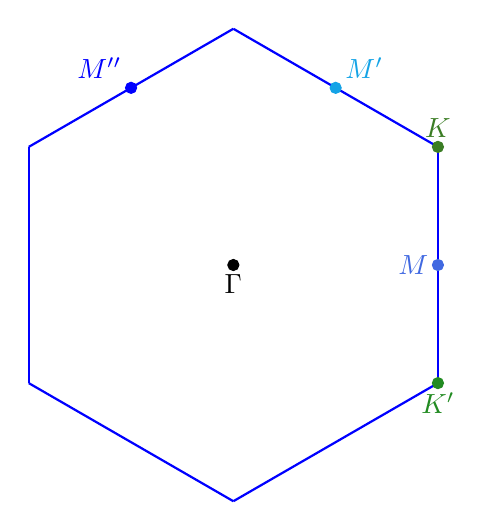
\begin{tikzpicture}
    \def\spacing{3} 
    \coordinate (A) at ({\spacing*cos(330)},{\spacing*sin(330)});
    \coordinate (B) at ({\spacing*cos(30)} ,{\spacing*sin(30)} );
    \coordinate (C) at ({\spacing*cos(90)},{\spacing*sin(90)});
    \coordinate (D) at ({\spacing*cos(150)},{\spacing*sin(150)});
    \coordinate (E) at ({\spacing*cos(210)},{\spacing*sin(210)});
    \coordinate (F) at ({\spacing*cos(270)},{\spacing*sin(270)});

    \draw[thick,blue] (A) -- (B);
    \draw[thick,blue] (B) -- (C);
    \draw[thick,blue] (C) -- (D);
    \draw[thick,blue] (D) -- (E);
    \draw[thick,blue] (E) -- (F);
    \draw[thick,blue] (F) -- (A);

    \newdimen\r
    \r=2pt

    % Gamma points
    \filldraw[black] (0,0) circle (\r) node[anchor=north] {$\Gamma$};

    % Dirac points
    \filldraw[ForestGreen] (A) circle (\r) node[anchor=north] {$K'$};
    
    \filldraw[OliveGreen] (B) circle (\r) node[anchor=south] {$K$};

    % M points
    \filldraw[RoyalBlue] (0:0.8660254038*\spacing) circle (\r) node[anchor=east] {$M$};
    \filldraw[Cerulean]  (60:0.8660254038*\spacing) circle (\r) node[anchor=south west] {$M'$};
    \filldraw[Blue] (120:0.8660254038*\spacing) circle (\r) node[anchor=south east] {$M''$};

  \end{tikzpicture}
  \caption{LEFT: All points of special interest shown on the lattice and how they are copied over to other lattice cells. RIGHT: Special points only in the first BZ since it has all the symmetries of the lattice}
  \label{fig:points}
\end{center}
\end{figure}
% Group theory (dihhedral group, little group)
% Average points of the same symmetry operation 
The primitive cell of the reciprocal lattice of the honeycomb is a hexagon, meaning it must have all the symmetries of the dihedral group. The result is that each set of momenta that is related by symmetry of the lattice can be averaged (e.g. $K$ with $K'$, $M$ with $M'$ and $M''$, etc.). The key moment here is that we have not used any model here. This is only due to the symmetry of the lattice itself. Therefore, this averaging of momenta could be performed anytime, but the group symmetry operations are lattice dependent (Square, Honeycomb, Kagome, and others).

\section{Symmetry Operators}
\label{sec:sym-oper}
In this section, we are going to focus only on transformation that do not change the Hamiltonian in general or at half filling ($\mu=0$) i.e. symmetry operations which means they commute with it 
\begin{equation}
  [H,R] = 0.
\end{equation}
We can show that the expectation value of the operator does not change when we apply the symmetry to it.
\begin{equation}
 \langle \mathcal{O} \rangle = \frac{1}{Z} tr[\mathcal{O}R^{-1}Re^{-\beta H}] = \frac{1}{Z} tr[\mathcal{O}R^{-1}e^{-\beta H}R] = \frac{1}{Z} tr[R\mathcal{O}R^{-1}e^{-\beta H}] = \langle R\mathcal{O}R^{-1} \rangle
\end{equation}
For our chosen model, there are only a few symmetry operators that satisfy this condition. We are going to see how they can be used to our advantage to increase our statistics~\cite{evan}.

% GIVE VISUAL EXAMPLES OF WHAT THE SYMMETRIES DO
\subsection{Spin-flip transformation}

On a bipartite lattice, we have a spin-flip operation that exchanges the particles and holes but leaves the charge untouched. On \cref{fig:spin-flip} there is shown an example of how the spin-flip operation transforms each operator when applied. Unfortunately, the example can show only how the spin and the charge transform, but not the Hamiltonian terms and amplitudes.
\begin{figure}
  \begin{center}
    \newcommand{\spinup}[2]{
    \draw[-Triangle , draw=#1, very thick] ([yshift=-1em]#2) -- ([yshift=1em]#2);
    }
    \newcommand{\spindown}[2]{
    \draw[Triangle- , draw=#1, very thick] ([yshift=-1em]#2) -- ([yshift=1em]#2);
    }
    \begin{tikzpicture}
      \tikzstyle{arrow} = [very thick,<->,>=stealth]
      \begin{scope}
        \def\spacing{3} 
        \coordinate (A) at ({\spacing}         ,{0}                  );
        \coordinate (B) at ({\spacing*cos(60)} ,{\spacing*sin(60)} );
        \coordinate (C) at ({\spacing*cos(120)},{\spacing*sin(120)});
        \coordinate (D) at ({-\spacing}         ,{0}                  );
        \coordinate (E) at ({\spacing*cos(240)},{\spacing*sin(240)});
        \coordinate (F) at ({\spacing*cos(300)},{\spacing*sin(300)});

        \draw[thin,dashed,black] (A) -- (B);
        \draw[thin,dashed,black] (B) -- (C);
        \draw[thin,dashed,black] (C) -- (D);
        \draw[thin,dashed,black] (D) -- (E);
        \draw[thin,dashed,black] (E) -- (F);
        \draw[thin,dashed,black] (F) -- (A);
        
        \spinup{blue}{A};
        \spinup{red}{B};
        \spindown{red}{C};
        \spinup{blue}{D};
        \spindown{blue}{E};
        \spindown{red}{F};
      \end{scope}

      \begin{scope}[xshift=9.5cm]
        \def\spacing{3} 
        \coordinate (A) at ({\spacing}         ,{0}                  );
        \coordinate (B) at ({\spacing*cos(60)} ,{\spacing*sin(60)} );
        \coordinate (C) at ({\spacing*cos(120)},{\spacing*sin(120)});
        \coordinate (D) at ({-\spacing}         ,{0}                  );
        \coordinate (E) at ({\spacing*cos(240)},{\spacing*sin(240)});
        \coordinate (F) at ({\spacing*cos(300)},{\spacing*sin(300)});
  
        \draw[thin,dashed,black] (A) -- (B);
        \draw[thin,dashed,black] (B) -- (C);
        \draw[thin,dashed,black] (C) -- (D);
        \draw[thin,dashed,black] (D) -- (E);
        \draw[thin,dashed,black] (E) -- (F);
        \draw[thin,dashed,black] (F) -- (A);
        
        \spindown{blue}{A};
        \spindown{red}{B};
        \spinup{red}{C};
        \spindown{blue}{D};
        \spinup{blue}{E};
        \spinup{red}{F};
      \end{scope}

      \draw[arrow] (3.5,0) -- (6,0) node [midway, sloped, above] {$I$};
    \end{tikzpicture}    
  \end{center}
  \caption{An example of the spin-flip transformation with all possibilities of creation/annihilation operators. The graphs show only the transformation of the charge and the spin of the operators. The color of the arrows shows the charge (blue = $+1$, red = $-1$) and the orientation shows the spin. We can go back and forth between the left and the right graphs by using the spin-flip conjugation.}
  \label{fig:spin-flip}
\end{figure}

When applied onto the creation/annihilation operators of the particles and the holes, this spin transformation gives us

\begin{align*}
  IpI^{-1} &= \Sigma h^\dagger = h^\dagger \Sigma & IhI^{-1} &= \Sigma p^\dagger = p^\dagger \Sigma \\
  Ip^\dagger I^{-1} &= \Sigma h = h \Sigma & Ih^\dagger I^{-1} &= \Sigma p = p \Sigma
\end{align*}
where $\Sigma$ is a matrix which shows us the behavior of the bipartite lattice
\begin{equation}
  \Sigma_{xy} = (-1)^x\delta_{xy}
\end{equation}
We can check if this symmetry commutes with the Hamiltonian by first showing that it leaves the charge invariant,
\begin{equation}
  IqI^{-1} = Ip^\dagger I^{-1}IpI^{-1} - Ih^\dagger I^{-1}IhI^{-1} = h\Sigma\Sigma h^\dagger - p\Sigma\Sigma p^\dagger = (1 - h^\dagger h) - (1 - p^\dagger p) = p^\dagger p - h^\dagger h = q
  \label{eq:spin-charge}
\end{equation}
It can also be shown that the third component of the spin gets flipped after we apply this operator
\begin{equation}
  Is^3I^{-1} = -s^3,
\end{equation}
where
\begin{equation}
  s^3_x = \frac{1}{2}\left(\delta_{xx} - p^\dagger_x p_x - h^\dagger_x h_x\right)
\end{equation}
Finally, it is important to see how the hopping term transforms under this symmetry operation
\begin{align*}
  I\left( -\sum_{xy} p^\dagger_x K_{xy} p_y + \sigma_k h^\dagger_x K_{xy} h_y\right) I^{-1} &= -\sum_{xy} I p^\dagger_x I^{-1}I K_{xy} I^{-1}I p_y I^{-1} + \sigma_k I h^\dagger_x I^{-1}I K_{xy} I^{-1}I h_y I^{-1}
  \\
  &= -\sum_{xy}  h_x (\Sigma I K I^{-1}\Sigma)_{xy} h^\dagger_y + \sigma_k p_x (\Sigma I K I^{-1}\Sigma)_{xy} p^\dagger_y
  \\
  &= -\sum_{xy} -(\delta_{xy} (I K I^{-1})_{xy} - h^\dagger_y (I K I^{-1})_{xy} h_x) -
  \\
  &- \sigma_k (\delta_{xy} (I K I^{-1})_{xy} - p^\dagger_y (I K I^{-1})_{xy} p_x)
  \\
  &= \sigma_k \left[-\sum_{xy} p^\dagger_x (I K I^{-1})^\top_{xy} p_y + \sigma_k h^\dagger_x (I K I^{-1})^\top_{xy} h_y \right]
\end{align*}
where $\Sigma K \Sigma = -K$, $tr[K] = 0$, and $\sigma^2_k = 1$. In general, to return to our initial hopping term, we need $I$ to be anti-unitary where $IKI^{-1} = K^*$, and then we could replace $K^\dagger\rightarrow K$. Since we are working on a bipartite lattice, $K$ is a real valued matrix, resulting in $IKI^{-1} = K$ and $K^\dagger = K^* = K^\top = K$; we can choose $\sigma_k = 1$ because of the Honeycomb, which even for $\mu \neq 0$ gives us the commutator $[H - \vec{\mu}\cdot\vec{q}, I] = 0$. This is true because as shown in (\cref{eq:spin-charge}) the charge is even in relation to the spin-flip symmetry operation.

\subsection{Charge transformation}

Another symmetry we can consider is the charge symmetry operation. It exchanges the charges but leaves the spin fixed. When applied onto the creation and annihilation operators, it transforms them as 
\begin{align*}
  CpC^{-1} &= h & ChC^{-1} &= p \\
  Cp^\dagger C^{-1} &= h^\dagger & Ch^\dagger C^{-1} &= p^\dagger
\end{align*}
On \cref{fig:charge-flip} is shown how the charge and spin of all creation/annihilation operators transform under this symmetry operation.
\begin{figure}
  \begin{center}
    \newcommand{\spinup}[2]{
    \draw[-Triangle , draw=#1, very thick] ([yshift=-1em]#2) -- ([yshift=1em]#2);
    }
    \newcommand{\spindown}[2]{
    \draw[Triangle- , draw=#1, very thick] ([yshift=-1em]#2) -- ([yshift=1em]#2);
    }
    \begin{tikzpicture}
      \tikzstyle{arrow} = [very thick,<->,>=stealth]
      \begin{scope}
        \def\spacing{3} 
        \coordinate (A) at ({\spacing}         ,{0}                  );
        \coordinate (B) at ({\spacing*cos(60)} ,{\spacing*sin(60)} );
        \coordinate (C) at ({\spacing*cos(120)},{\spacing*sin(120)});
        \coordinate (D) at ({-\spacing}         ,{0}                  );
        \coordinate (E) at ({\spacing*cos(240)},{\spacing*sin(240)});
        \coordinate (F) at ({\spacing*cos(300)},{\spacing*sin(300)});

        \draw[thin,dashed,black] (A) -- (B);
        \draw[thin,dashed,black] (B) -- (C);
        \draw[thin,dashed,black] (C) -- (D);
        \draw[thin,dashed,black] (D) -- (E);
        \draw[thin,dashed,black] (E) -- (F);
        \draw[thin,dashed,black] (F) -- (A);
        
        \spinup{blue}{A};
        \spinup{red}{B};
        \spindown{red}{C};
        \spinup{blue}{D};
        \spindown{blue}{E};
        \spindown{red}{F};
      \end{scope}

      \begin{scope}[xshift=9.5cm]
        \def\spacing{3} 
        \coordinate (A) at ({\spacing}         ,{0}                  );
        \coordinate (B) at ({\spacing*cos(60)} ,{\spacing*sin(60)} );
        \coordinate (C) at ({\spacing*cos(120)},{\spacing*sin(120)});
        \coordinate (D) at ({-\spacing}         ,{0}                  );
        \coordinate (E) at ({\spacing*cos(240)},{\spacing*sin(240)});
        \coordinate (F) at ({\spacing*cos(300)},{\spacing*sin(300)});
  
        \draw[thin,dashed,black] (A) -- (B);
        \draw[thin,dashed,black] (B) -- (C);
        \draw[thin,dashed,black] (C) -- (D);
        \draw[thin,dashed,black] (D) -- (E);
        \draw[thin,dashed,black] (E) -- (F);
        \draw[thin,dashed,black] (F) -- (A);
        
        \spinup{red}{A};
        \spinup{blue}{B};
        \spindown{blue}{C};
        \spinup{red}{D};
        \spindown{red}{E};
        \spindown{blue}{F};
      \end{scope}

      \draw[arrow] (3.5,0) -- (6,0) node [midway, sloped, above] {$C$};
    \end{tikzpicture}
  \end{center}
  \caption{An example of the charge transformation with all possibilities of creation/annihilation operators. The graphs show only the transformation of the charge and the spin of the operators. The color of the arrows shows the charge (blue = $+1$, red = $-1$) and the orientation shows the spin. We can go back and forth between the left and the right graphs by using the charge-flip conjugation.}
  \label{fig:charge-flip}
\end{figure}
If we conjugate with the charge operator, we get
\begin{equation}
  CqC^{-1} = Cp^\dagger C^{-1}CpC^{-1} - Ch^\dagger C^{-1}ChC^{-1} = h^\dagger h - p^\dagger p = -q
  \label{eq:charge-charge}
\end{equation}
and when conjugated with the spin operator
\begin{equation}
  Cs^3C^{-1} = s^3,
\end{equation}
so the spin is fixed for this operation. Again, we want to calculate the conjugation of the tight-binding term in the Hamiltonian with the charge-flip operator

\begin{align*}
  C\left( -\sum_{xy} p^\dagger_x K_{xy} p_y + \sigma_k h^\dagger_x K_{xy} h_y\right) C^{-1} &= -\sum_{xy} C p^\dagger_x C^{-1}C K_{xy} C^{-1}C p_y C^{-1} + \sigma_k C h^\dagger_x C^{-1}C K_{xy} C^{-1}C h_y C^{-1}
  \\
  &= -\sum_{xy}  h^\dagger_x (C K C^{-1})_{xy} h_y + \sigma_k p^\dagger_x (C K C^{-1})_{xy} p_y
  \\
  &= -\sum_{xy}  \sigma_k p^\dagger_x (C K C^{-1})_{xy} p_y + h^\dagger_x (C K C^{-1})_{xy} h_y
\end{align*}
where if we choose $CKC^{-1} = K$, we get to the initial term. Therefore, we are shown that on a bipartite lattice where we can choose $\sigma_k = +1$, we have a charge conjugation symmetry i.e. it commutes with the tight-binding Hamiltonian $[H,C] = 0$. This is because as shown in (\cref{eq:charge-charge}) the charge operator is flipped, but the interaction is even under this transformation because it is of the form $qVq$.

\subsection{Particle-hole transformation}

The particle-hole symmetry operator is a combination of two symmetry operators that do not transform the Hamiltonian nicely, but their combination does. It preserves the energy of the system, but flips the charge and the spin. This means that we should only consider the tight-binding Hamiltonian, i.e. the Hamiltonian without the chemical potential term.

In order to convince ourselves of the neat transformation and also the commutation of the Hamiltonian with the symmetry operator, we should first see how the constituent operators transform the Hubbard model Hamiltonian.

First, we look at the staggering operator $X$. It transforms the creation/annihilation operators like
\begin{align*}
  Xp^\dagger X^{-1} &= \Sigma p^\dagger = p^\dagger \Sigma & Xh^\dagger X^{-1} &= \Sigma h^\dagger = h^\dagger \Sigma \\
  Xp X^{-1} &= \Sigma p = p \Sigma & XhX^{-1} &= \Sigma h = h \Sigma
\end{align*}
It leaves the charge, spin, and number operators invariant, but it flips the sign of the hopping term

\begin{align*}
  X\left( -\sum_{xy} p^\dagger_x K_{xy} p_y + \sigma_k h^\dagger_x K_{xy} h_y\right) X^{-1} &= -\sum_{xy} X p^\dagger_x X^{-1}X K_{xy} X^{-1}X p_y X^{-1} + \sigma_k X h^\dagger_x X^{-1}X K_{xy} X^{-1}X h_y X^{-1}
  \\
  &= -\sum_{xy}  p^\dagger_x (\Sigma X K X^{-1}\Sigma)_{xy} p_y + \sigma_k h^\dagger_x (\Sigma X K X^{-1}\Sigma)_{xy} h_y
  \\
  &= -\sum_{xy}  p^\dagger_x (\Sigma K \Sigma)_{xy} p_y + \sigma_k h^\dagger_x (\Sigma K \Sigma)_{xy} h_y
  \\
  &= -\left[-\sum_{xy} p^\dagger_x K_{xy} p_y + \sigma_k h^\dagger_x K_{xy} h_y \right]
\end{align*}

The other operator that we consider is the one that "flips" the dagger of the operators. It transforms the particle/hole operators as

\begin{align*}
  FpF^{-1} &= p^\dagger & FhF^{-1} &= h^\dagger \\
  Fp^\dagger F^{-1} &= p & Fh^\dagger F^{-1} &= h
\end{align*}

When applied onto the charge operator, it flips the sign $q \rightarrow -q$ which is shown below

\begin{equation}
  FqF^{-1} = Fp^\dagger F^{-1}FpF^{-1} - Fh^\dagger F^{-1}FhF^{-1} = p p^\dagger - h h^\dagger = (1 - p^\dagger p) - (1 - h^\dagger h) = -q
\end{equation}
This in turn means that this symmetry operation flips the chemical potential and more importantly the hopping term
\begin{align*}
  F\left( -\sum_{xy} p^\dagger_x K_{xy} p_y + \sigma_k h^\dagger_x K_{xy} h_y\right) F^{-1} &= -\sum_{xy} F p^\dagger_x F^{-1}F K_{xy} F^{-1}F p_y F^{-1} + \sigma_k F h^\dagger_x F^{-1}F K_{xy} F^{-1}F h_y F^{-1}
  \\
  &= -\sum_{xy}  p_x (F K F^{-1})_{xy} p^\dagger_y + \sigma_k h_x (F K F^{-1})_{xy} h^\dagger_y
  \\
  &= -\sum_{xy} (\delta_{xy} (F K F^{-1})_{xy} - p^\dagger_y (F K F^{-1})_{xy} p_x) + \sigma_k (\delta_{xy} (F K F^{-1})_{xy} - h^\dagger_y (F K F^{-1})_{xy} h_x)
  \\
  &= - \left[ - \sum_{xy} p^\dagger_y (F K F^{-1})_{xy} p_x + \sigma_k h^\dagger_y (F K F^{-1})_{xy} h_x \right]
  \\
  &= - \left[ - \sum_{xy} p^\dagger_x (F K F^{-1})^\top_{xy} p_y + \sigma_k h^\dagger_x (F K F^{-1})^\top_{xy} h_y \right]
\end{align*}
where $tr[K] = 0$, if we want to return to the original hopping term then we have to choose $F K F^{-1} = K^*$, and then we can substitute $K^\dagger \rightarrow K$. We see on  \cref{fig:dagger-flip} an example of the dagger-flip operator switching the signs of the charge and the spin.
\begin{figure}
  \begin{center}
    \newcommand{\spinup}[2]{
    \draw[-Triangle , draw=#1, very thick] ([yshift=-1em]#2) -- ([yshift=1em]#2);
    }
    \newcommand{\spindown}[2]{
    \draw[Triangle- , draw=#1, very thick] ([yshift=-1em]#2) -- ([yshift=1em]#2);
    }
    \begin{tikzpicture}
      \tikzstyle{arrow} = [very thick,<->,>=stealth]
      \begin{scope}
        \def\spacing{3} 
        \coordinate (A) at ({\spacing}         ,{0}                  );
        \coordinate (B) at ({\spacing*cos(60)} ,{\spacing*sin(60)} );
        \coordinate (C) at ({\spacing*cos(120)},{\spacing*sin(120)});
        \coordinate (D) at ({-\spacing}         ,{0}                  );
        \coordinate (E) at ({\spacing*cos(240)},{\spacing*sin(240)});
        \coordinate (F) at ({\spacing*cos(300)},{\spacing*sin(300)});

        \draw[thin,dashed,black] (A) -- (B);
        \draw[thin,dashed,black] (B) -- (C);
        \draw[thin,dashed,black] (C) -- (D);
        \draw[thin,dashed,black] (D) -- (E);
        \draw[thin,dashed,black] (E) -- (F);
        \draw[thin,dashed,black] (F) -- (A);
        
        \spinup{blue}{A};
        \spinup{red}{B};
        \spindown{red}{C};
        \spinup{blue}{D};
        \spindown{blue}{E};
        \spindown{red}{F};
      \end{scope}

      \begin{scope}[xshift=9.5cm]
        \def\spacing{3} 
        \coordinate (A) at ({\spacing}         ,{0}                  );
        \coordinate (B) at ({\spacing*cos(60)} ,{\spacing*sin(60)} );
        \coordinate (C) at ({\spacing*cos(120)},{\spacing*sin(120)});
        \coordinate (D) at ({-\spacing}         ,{0}                  );
        \coordinate (E) at ({\spacing*cos(240)},{\spacing*sin(240)});
        \coordinate (F) at ({\spacing*cos(300)},{\spacing*sin(300)});
  
        \draw[thin,dashed,black] (A) -- (B);
        \draw[thin,dashed,black] (B) -- (C);
        \draw[thin,dashed,black] (C) -- (D);
        \draw[thin,dashed,black] (D) -- (E);
        \draw[thin,dashed,black] (E) -- (F);
        \draw[thin,dashed,black] (F) -- (A);
        
        \spindown{red}{A};
        \spindown{blue}{B};
        \spinup{blue}{C};
        \spindown{red}{D};
        \spinup{red}{E};
        \spinup{blue}{F};
      \end{scope}

      \draw[arrow] (3.5,0) -- (6,0) node [midway, sloped, above] {$F$};
    \end{tikzpicture}
  \end{center}
  \caption{An example of the dagger-flip transformation with all possibilities of creation/annihilation operators. The graphs show only the transformation of the charge and the spin of the operators. The color of the arrows shows the charge (blue = $+1$, red = $-1$) and the orientation shows the spin. We can go back and forth between the left and the right graphs by using the dagger-flip conjugation.}
  \label{fig:dagger-flip}
\end{figure}

After we have shown how the different term of the Hamiltonian transform under both symmetries separately, we can answer how the composition of the two transforms each term of the Hubbard model's Hamiltonian. Starting from the hopping term, we know that each operation flips the sign of the kinetic term, meaning it is even under the composed operator. Next, we know that the charge operator is invariant under the staggering operator, and it flips sign when conjugated with the dagger-flip operator. This means that the interaction term $qVq$ must preserve its sign with the particle-hole transformation because the interaction is bilinear. Finally, the chemical potential unfortunately is linear $\vec{\mu}\cdot \vec{q}$, so the sign of this term is flipped. After all these considerations, we could conclude that at half-filling ($\mu = 0$), the tight-binding Hamiltonian commutes with the particle-hole transformation
\begin{equation}
  [H, XF] = 0,
\end{equation} 
and we can use this symmetry operation to our advantage. On  \cref{fig:ph-flip} it is shown again an example of the transformation of spin and charge. On this graph, we can only visualize the spin and the charge of the operators but not the transformed terms of the Hamiltonian, resulting in the same looking example as if only we consider $F$ in spite of the kinetic terms having opposite signs.
\begin{figure}
  \begin{center}
    \newcommand{\spinup}[2]{
    \draw[-Triangle , draw=#1, very thick] ([yshift=-1em]#2) -- ([yshift=1em]#2);
    }
    \newcommand{\spindown}[2]{
    \draw[Triangle- , draw=#1, very thick] ([yshift=-1em]#2) -- ([yshift=1em]#2);
    }
    \begin{tikzpicture}
      \tikzstyle{arrow} = [very thick,<->,>=stealth]
      \begin{scope}
        \def\spacing{3} 
        \coordinate (A) at ({\spacing}         ,{0}                  );
        \coordinate (B) at ({\spacing*cos(60)} ,{\spacing*sin(60)} );
        \coordinate (C) at ({\spacing*cos(120)},{\spacing*sin(120)});
        \coordinate (D) at ({-\spacing}         ,{0}                  );
        \coordinate (E) at ({\spacing*cos(240)},{\spacing*sin(240)});
        \coordinate (F) at ({\spacing*cos(300)},{\spacing*sin(300)});

        \draw[thin,dashed,black] (A) -- (B);
        \draw[thin,dashed,black] (B) -- (C);
        \draw[thin,dashed,black] (C) -- (D);
        \draw[thin,dashed,black] (D) -- (E);
        \draw[thin,dashed,black] (E) -- (F);
        \draw[thin,dashed,black] (F) -- (A);
        
        \spinup{blue}{A};
        \spinup{red}{B};
        \spindown{red}{C};
        \spinup{blue}{D};
        \spindown{blue}{E};
        \spindown{red}{F};
      \end{scope}

      \begin{scope}[xshift=9.5cm]
        \def\spacing{3} 
        \coordinate (A) at ({\spacing}         ,{0}                  );
        \coordinate (B) at ({\spacing*cos(60)} ,{\spacing*sin(60)} );
        \coordinate (C) at ({\spacing*cos(120)},{\spacing*sin(120)});
        \coordinate (D) at ({-\spacing}         ,{0}                  );
        \coordinate (E) at ({\spacing*cos(240)},{\spacing*sin(240)});
        \coordinate (F) at ({\spacing*cos(300)},{\spacing*sin(300)});
  
        \draw[thin,dashed,black] (A) -- (B);
        \draw[thin,dashed,black] (B) -- (C);
        \draw[thin,dashed,black] (C) -- (D);
        \draw[thin,dashed,black] (D) -- (E);
        \draw[thin,dashed,black] (E) -- (F);
        \draw[thin,dashed,black] (F) -- (A);
        
        \spindown{red}{A};
        \spindown{blue}{B};
        \spinup{blue}{C};
        \spindown{red}{D};
        \spinup{red}{E};
        \spinup{blue}{F};
      \end{scope}

      \draw[arrow] (3.5,0) -- (6,0) node [midway, sloped, above] {$XF$};
    \end{tikzpicture}
  \end{center}
  \caption{An example of the particle-hole transformation with all possibilities of creation/annihilation operators. The graphs show only the transformation of the charge and the spin of the operators. The color of the arrows shows the charge (blue = $+1$, red = $-1$) and the orientation shows the spin. We can go back and forth between the left and the right graphs by using the particle-hole conjugation.}
  \label{fig:ph-flip}
\end{figure}

It is worth noting that after working out how these symmetry operations transform the Hamiltonian, we could write out $I = XFC$, but we should still examine them all separately because $I$ commutes with the whole Hamiltonian and the other two only with the tight-binding one.

% \def\hexagonsize{1cm}
% \pgfdeclarepatternformonly
%   {hexagons}% name
%   {\pgfpointorigin}% lower left
%   {\pgfpoint{3*\hexagonsize}{0.866025*2*\hexagonsize}}%  upper right
%   {\pgfpoint{3*\hexagonsize}{0.866025*2*\hexagonsize}}%  tile size
%   {% shape description
%    \pgfsetlinewidth{0.4pt}
%    \pgftransformshift{\pgfpoint{0mm}{0.866025*\hexagonsize}}
%    \pgfpathmoveto{\pgfpoint{0mm}{0mm}}
%    \pgfpathlineto{\pgfpoint{0.5*\hexagonsize}{0mm}}
%    \pgfpathlineto{\pgfpoint{\hexagonsize}{-0.866025*\hexagonsize}}
%    \pgfpathlineto{\pgfpoint{2*\hexagonsize}{-0.866025*\hexagonsize}}
%    \pgfpathlineto{\pgfpoint{2.5*\hexagonsize}{0mm}}
%    \pgfpathlineto{\pgfpoint{3*\hexagonsize+0.2mm}{0mm}}
%    \pgfpathmoveto{\pgfpoint{0.5*\hexagonsize}{0mm}}
%    \pgfpathlineto{\pgfpoint{\hexagonsize}{0.866025*\hexagonsize}}
%    \pgfpathlineto{\pgfpoint{2*\hexagonsize}{0.866025*\hexagonsize}}
%    \pgfpathlineto{\pgfpoint{2.5*\hexagonsize}{0mm}}
%    \pgfusepath{stroke}
%   }

%   \begin{tikzpicture}
%     \fill[pattern=hexagons] (0,0) rectangle (10,5);
%     \end{tikzpicture}
    
%     \begin{tikzpicture}
%     \fill[pattern=hexagons] (0,0) circle (3cm);
%     \end{tikzpicture}

%     \tikzset
%     {tri/.style = % red triangles (needs shapes.geometric)
%       {draw=red,fill=red,isosceles triangle,isosceles triangle stretches,
%        shape border rotate=90,minimum width=0.2cm,minimum height=0.2cm,
%        inner sep=0pt
%       },
%      box/.style = % black squares
%       {draw=black,fill=black,rectangle,minimum width=0.2cm,
%        minimum height=0.2cm,inner sep=0pt
%       }
%     }
%   \begin{tikzpicture}[x=0.1mm,y=0.1mm]
%     \newcommand\side{57.735} % hex side = hex height / (2*sin(60)) = hex height / sqrt(3)
%     \begin{scope}[draw=blue] % scope for hexagon grid
%       \clip (0,0) rectangle (1000,501); % clipping confines grid to rectangle
%       \foreach \i in {0,...,6} % seven towers of hexagons
%         \foreach \j in {0,...,5} % each six hexagons high
%           {\begin{scope}[shift={({\i*3*\side},{\j*100})}] % scope for one hexagon
%             \foreach \k in {0,60,...,300}
%               \draw (\k:\side) -- ({\k+60}:\side); % draw hexagon using polar coordinates
%             \draw (\side,0) -- ({2*\side},0); % draw a horizontal extender connecting neighboring hexagon towers
%            \end{scope}
%           }
%     \end{scope}

%     % marks
%     \node[tri] at ({2*\side},300) {};
%     \node[tri] at ({2.5*\side},450) {};
%     \node[box] at ({3.5*\side},250) {};
%     \node[tri] at ({4*\side},100) {};
%     \node[tri] at ({5.5*\side},150) {};
%     \node[tri] at ({5.5*\side},250) {};
%     \node[tri] at ({8.5*\side},50) {};
%     \node[tri] at ({10*\side},400) {};
%     \node[tri] at ({11.5*\side},450) {};
%     \node[tri] at ({11.5*\side},350) {};
%     \node[box] at ({12.5*\side},250) {};
%     \node[tri] at ({17*\side},100) {};
%   \end{tikzpicture}
  
\section{Correlation functions}
\label{sec:sym-corr}

After we have found out what the symmetries of the lattice in \cref{sec:lattice} are and how they transform the relevant operators, we can take them into consideration and apply them onto the one- and two-body correlation functions (\cref{sec:corr_func}). We use them in order to average data with the same total momentum. This will increase our statistics and better our precision when performing the fitting of the final data.

\subsection{One-particle correlation function}
% How do I write about the Evan's paper which is not yet published. It is still a work in progress.

First, we start with the one-body correlators which will give us a valuable insight on how to work with the two-body correlation functions. The full derivation is provided in \cite{evan}, so only the relevant information for this thesis will be shown here.

% We start with the $\langle p_\tau p^\dagger_0 \rangle$, where the indices indicate on which timesslice the operators live. The source can always be placed on the 0th timeslice since there is a time translational invariance. We write this correlation function as $C_Q=+1,S=1,S^3=-1,\vec{k}$.
We start with the $\langle pp^\dagger \rangle$ correlation function which we can write as $C_Q=+1,S=1,S^3=-1,\vec{k}$. It can be represented as a $2\times 2$ matrix with two one-body correlators due to the internal band labels
\newcommand{\corp}[2]{p_{#1}p^\dagger_{#2}}
\begin{equation}
  C_{Q=+1,S=1,S^3=-1,\vec{k}} =
  \left[
  \begin{array}{cc}
    \corp{+}{+} & \corp{+}{-} \\
    \corp{-}{+} & \corp{-}{-}
  \end{array}
  \right] _{\vec{k}} (\tau)
\end{equation}
This matrix of correlators can be calculated and then diagonalized to
\begin{equation}
  C_{Q=+1,S=1,S^3=-1,\vec{k}} = \frac{1}{2}\left(C_{\corp{+}{+}} + C_{\corp{-}{-}}\right)\mathds{1} + \frac{1}{2}\left(\sqrt{\left(C_{\corp{+}{+}} - C_{\corp{-}{-}}\right)^2 + 4 C_{\corp{+}{-}}C_{\corp{-}{+}}}\right)\sigma_3
\end{equation}
In the tight-binding case of the Hamiltonian, the off-diagonal components vanish and the diagonal are equal. However, in general one must be careful because this is discretization dependent. In order to avoid this problem, we must always compute the whole matrix and then diagonalize. The whole argument can also be done for $\langle hh^\dagger\rangle$.

To increase the precision of our data, we apply the symmetry operators that we calculated in  \cref{sec:sym-oper}. Also, we use the cyclic property of the trace, and the final results can be seen in \cref{tab:1psym}. A detailed derivation of these results as mentioned previously can be found in \cite{evan}. It is important to note that we can increase the precision up to eightfold not sixteenfold which is the number of cases in the table. This is because some entries are duplicates, and they can be found by examining the quantum numbers in the second column. The averaging put into equations looks like this
\begin{equation}
  \tilde{C}_{QS^3\vec{k}}(\tau) = \frac{1}{4}\left( C_{QS^3\vec{k}}(\tau) + C_{\overline{QS^3}\vec{k}}(\beta-\tau)^\top + \sigma_1\cdot C_{Q\overline{S^3}\vec{k}}(\tau) \cdot\sigma_1 + \sigma_1\cdot C_{\overline{Q}S^3\vec{k}}(\beta-\tau)^\top \cdot\sigma_1 \right)
  \label{eq:average}
\end{equation}
and
\begin{equation}
  \tilde{C}_{\vec{k}}(\tau) = \frac{1}{2}\left( \tilde{C}_{QS^3\vec{k}}(\tau) + \tilde{C}_{\overline{Q}S^3\vec{k}}(\tau) \right)
  \label{eq:full_average}
\end{equation}
We could always use \cref{eq:average} to average and be four times more precise and only when $\mu = 0$, we can also use \cref{eq:full_average} for a total of eight times more statistics. After that, one must always diagonalize.
% In Subsection \cref{ssec:sym-twobody} we will derive the 

% WRITE OUT THE SYMMETRY TABLE  HERE (Continue...)
\begin{table}[h]
  \centering
  \begin{tabular}{cc|ccccc}
             & & $Q$ & $S$ & $S^3$ & $\vec{k}$ & $\tau$  \\
  \hline
  Start with & $QSkt$ & +1 & $\frac{1}{2}$ & $-\frac{1}{2}$ & 1 & $\tau$ \\
  \hline
  trace cycl & $\overline{QSkt}$ & -1 & $\frac{1}{2}$ & $+\frac{1}{2}$ & $\top$ & $\beta-\tau$ \\
  \hline
  I          & $Q\overline{Sk}t$ & +1 & $\frac{1}{2}$ & $+\frac{1}{2}$ & $\sigma_1\cdot\sigma_1$ & $\tau$ \\
             & & -1 & $\frac{1}{2}$ & $-\frac{1}{2}$ & $\sigma_1\top\sigma_1$ & $\beta-\tau$ \\
  \hline\hline
  XF         & $\overline{QSk}t$ & -1 & $\frac{1}{2}$ & $+\frac{1}{2}$ & $\sigma_1\cdot\sigma_1$ & $\tau$ \\
             & & +1 & $\frac{1}{2}$ & $-\frac{1}{2}$ & $\sigma_1\cdot\sigma_1$ & $\beta-\tau$ \\
             & & -1 & $\frac{1}{2}$ & $-\frac{1}{2}$ & 1 & $\tau$ \\
             & & +1 & $\frac{1}{2}$ & $+\frac{1}{2}$ & $\top$ & $\beta-\tau$ \\
  \hline
  C          & $\overline{Q}Skt$ & -1 & $\frac{1}{2}$ & $-\frac{1}{2}$ & 1 & $\tau$ \\
             & & +1 & $\frac{1}{2}$ & $+\frac{1}{2}$ & $\top$ & $\beta-\tau$ \\
             & & -1 & $\frac{1}{2}$ & $+\frac{1}{2}$ & $\sigma_1\cdot\sigma_1$ & $\tau$ \\
             & & +1 & $\frac{1}{2}$ & $-\frac{1}{2}$ & $\sigma_1\top\sigma_1$ & $\beta-\tau$ \\
             & & +1 & $\frac{1}{2}$ & $+\frac{1}{2}$ & $\sigma_1\cdot\sigma_1$ & $\tau$ \\
             & & -1 & $\frac{1}{2}$ & $-\frac{1}{2}$ & $\sigma_1\top\sigma_1$ & $\beta-\tau$ \\
             & & +1 & $\frac{1}{2}$ & $-\frac{1}{2}$ & 1 & $\tau$ \\
             & & -1 & $\frac{1}{2}$ & $+\frac{1}{2}$ & $\top$ & $\beta-\tau$
  \end{tabular}
  \caption{All the correlators that can be directly averaged, assuming they all take the $2 \times 2$ matrix form. The correlators above the double line may be averaged even at finite $\mu$ and everything below may be averaged when $\mu = 0$. The combination of charge and spin indicate whether $p^\dagger$, $p$, $h^\dagger$, or $h$ is right-most. The $\vec{k}$ column indicates what must be done in the internal $2 \times 2$ momentum space before averaging; $\top$ indicates transpose, $\sigma_1\cdot\sigma_1$ indicates conjugation by $\sigma_1$, $1$ indicates that no operation is needed. The $\tau$ column indicates whether the given correlator needs to be time-reversed.}
  \label{tab:1psym}
\end{table}

\subsection{Two-particle correlation function}
\label{ssec:sym-twobody}
In this thesis, we are working with only two types of two-body correlators. There are correlators with particles and holes, and only particles. We start with the former correlator $\langle phh^\dagger p^\dagger\rangle$. In matrix form with all labels it looks like this

\newcommand{\cor}[4]{p_{#1}h_{#2}h^\dagger_{#3}p^\dagger_{#4}}
\begin{equation}
  C_{Q=0,S=1,S^3=-1;k,q,r,s} =
  \left[
  \begin{array}{cccc}
    \cor{+}{+}{+}{+} & \cor{+}{+}{+}{-} & \cor{+}{+}{-}{+} & \cor{+}{+}{-}{-} \\
    \cor{+}{-}{+}{+} & \cor{+}{-}{+}{-} & \cor{+}{-}{-}{+} & \cor{+}{-}{-}{-} \\
    \cor{-}{+}{+}{+} & \cor{-}{+}{+}{-} & \cor{-}{+}{-}{+} & \cor{-}{+}{-}{-} \\
    \cor{-}{-}{+}{+} & \cor{-}{-}{+}{-} & \cor{-}{-}{-}{+} & \cor{-}{-}{-}{-} \\
  \end{array}
  \right]_{k,q,r,s} (\tau)
  \label{eq:phhpmat}
\end{equation}
Now, we apply a different symmetry operator to the two particle correlation function. The derivations of the conjugation with the symmetry operators are always done in two steps. First, we start with the thermal trace and then switch to matrix form, so that it is easier to see the transformations needed in order to get another two particle correlator.
\\
\\
\subsubsection{\underline{Trace Cyclicity}}
We begin with the trace cyclicity, because it will give us how the correlation function transformations when time reversed.
\\
\begin{equation}
  C_{Q=0,S=1,S^3=-1;k,q,r,s} = \frac{1}{Z}tr\left[p_kh_qe^{-H\tau}h^\dagger_rp^\dagger_se^{-H\left(\beta-\tau\right)}\right] =\
  \frac{1}{Z}tr\left[h^\dagger_rp^\dagger_se^{-H\left(\beta-\tau\right)}p_kh_qe^{-H\tau}\right]
\end{equation}
Now we apply time reverse
$$\beta \rightarrow \beta - \tau$$
and use the anti-commutation relations of the operators to get
\begin{equation}
  \frac{1}{Z}tr\left[h^\dagger_rp^\dagger_se^{-H\left(\beta-\left(\beta-\tau\right)\right)}p_kh_qe^{-H\left(\beta-\tau\right)}\right]=\\\
  \frac{1}{Z}tr\left[p^\dagger_sh^\dagger_re^{-H\tau}h_qp_ke^{-H\left(\beta-\tau\right)}\right]
\end{equation}
We switch to matrix form to see observe better how all labels transform

\renewcommand{\cor}[4]{p_{#1}h_{#2}h^\dagger_{#3}p^\dagger_{#4}}
\newcommand{\dcor}[4]{h_{#3}^\dagger p_{#4}^\dagger p_{#1} h_{#2}}
\begin{equation}
  \begin{aligned}
    &C_{Q=0,S=1,S^3=-1;k,q,r,s} \\
    &= \left[ 
    {\begin{array}{cccc}
      \cor{+}{+}{+}{+} & \cor{+}{+}{+}{-} & \cor{+}{+}{-}{+} & \cor{+}{+}{-}{-} \\
      \cor{+}{-}{+}{+} & \cor{+}{-}{+}{-} & \cor{+}{-}{-}{+} & \cor{+}{-}{-}{-} \\
      \cor{-}{+}{+}{+} & \cor{-}{+}{+}{-} & \cor{-}{+}{-}{+} & \cor{-}{+}{-}{-} \\
      \cor{-}{-}{+}{+} & \cor{-}{-}{+}{-} & \cor{-}{-}{-}{+} & \cor{-}{-}{-}{-} \\
    \end{array} } \right]_{k,q,r,s} (\tau) \\
    &= \left[ 
    {\begin{array}{cccc}
      \dcor{+}{+}{+}{+} & \dcor{+}{+}{+}{-} & \dcor{+}{+}{-}{+} & \dcor{+}{+}{-}{-} \\
      \dcor{+}{-}{+}{+} & \dcor{+}{-}{+}{-} & \dcor{+}{-}{-}{+} & \dcor{+}{-}{-}{-} \\
      \dcor{-}{+}{+}{+} & \dcor{-}{+}{+}{-} & \dcor{-}{+}{-}{+} & \dcor{-}{+}{-}{-} \\
      \dcor{-}{-}{+}{+} & \dcor{-}{-}{+}{-} & \dcor{-}{-}{-}{+} & \dcor{-}{-}{-}{-} \\
    \end{array} } \right]_{r,s,k,q} (\beta-\tau) \\
  \end{aligned}
\end{equation}

\renewcommand{\dcor}[4]{p_{#4}^\dagger h_{#3}^\dagger h_{#2} p_{#1}}

\begin{equation}
  \begin{aligned}
    &= \left[ 
    \begin{array}{cccc}
      \dcor{+}{+}{+}{+} & \dcor{+}{+}{+}{-} & \dcor{+}{+}{-}{+} & \dcor{+}{+}{-}{-} \\
      \dcor{+}{-}{+}{+} & \dcor{+}{-}{+}{-} & \dcor{+}{-}{-}{+} & \dcor{+}{-}{-}{-} \\
      \dcor{-}{+}{+}{+} & \dcor{-}{+}{+}{-} & \dcor{-}{+}{-}{+} & \dcor{-}{+}{-}{-} \\
      \dcor{-}{-}{+}{+} & \dcor{-}{-}{+}{-} & \dcor{-}{-}{-}{+} & \dcor{-}{-}{-}{-} \\
    \end{array} \right]_{s,r,q,k} (\beta-\tau) \\
    &= C_{Q=0,S=1,S^3=+1;s,r,q,k}
  \end{aligned}
\end{equation}
We notice that order reverse is actually composed of two transformations -- particle-hole momentum switch and time reverse. After we stare at the matrix for an hour, we can figure out what the transformation between the correlation functions is
\begin{equation}
  C_{Q=0,S=1,S^3=-1;k,q,r,s} (\tau) =
  \left[ {\begin{array}{cccc}
    1 & 0 & 0 & 0 \\
    0 & 0 & 1 & 0 \\
    0 & 1 & 0 & 0 \\
    0 & 0 & 0 & 1 \\
  \end{array} } \right]
  {C_{Q=0,S=1,S^3=+1;s,r,q,k}}^\top (\beta-\tau)
  \left[ {\begin{array}{cccc}
    1 & 0 & 0 & 0 \\
    0 & 0 & 1 & 0 \\
    0 & 1 & 0 & 0 \\
    0 & 0 & 0 & 1 \\
  \end{array} } \right]
\end{equation}

We repeat the steps again for each symmetry operator. First, we start with the thermal trace and then switch to matrix for easy transformations.   \cref{tab:phhp} shows the summary of all symmetries that we have calculated for $\langle phh^\dagger p^\dagger \rangle$ (see \cref{sec:app}).

\begin{table}[h]
  \centering
  \begin{tabular}{c|cccccc}
             & $Q$ & $S$ & $S^3$ & trafo & $kqrs$    & $\tau$  \\
  \hline
  Start with & 0 & 1 & -1 & 1 & 1234 &  $\tau$  \\
  \hline
  trace cycl & 0 & 1 & +1 & $\sigma_5 \top \sigma_5$ & 4321 & $\beta-\tau$ \\
  \hline
  I          & 0 & 1 & -1 & $\sigma_1 \top \sigma_1$ & 3412 & $\beta-\tau$ \\
             & 0 & 1 & +1 & $\sigma_5\sigma_1\cdot\sigma_1\sigma_5$ & 2143 & $\tau$ \\
  \hline\hline
  C          & 0 & 1 & +1 & $\top$ & 3412 & $\beta-\tau$ \\
             & 0 & 1 & -1 & $\sigma_5\cdot\sigma_5$ & 2143 & $\tau$ \\
  \hline
  XF         & 0 & 1 & +1 & $\sigma_1\cdot\sigma_1$ & 1234 & $\tau$ \\
             & 0 & 1 & -1 & $\sigma_5\sigma_1\top\sigma_1\sigma_5$ & 4321 & $\beta-\tau$
  \end{tabular}
  \caption{All the correlators that can be directly averaged, if they all take a $4 \times 4$ matrix form. The correlators above the double line may be averaged even at finite $\mu$ and everything below may be averaged when $\mu = 0$. The combination of charge and spin indicate whether $h^\dagger p^\dagger$ or $hp$ is at the source (right-most). The \textit{trafo} column indicates what must be done in the internal $4 \times 4$ momentum space before averaging; $\top$ indicates transpose, $\sigma_1\cdot\sigma_1$ indicates conjugation by $\sigma_1$, $\sigma_5\cdot\sigma_5$ indicates conjugation by $\sigma_5$, and $1$ indicates that no operation is needed. The next column $kqrs$ indicates the position of the momenta at the sink and source relative to the initial correlator is. The $\tau$ column indicates whether the given correlator needs to be time-reversed.}
  \label{tab:phhp}
\end{table}

For more compact form, we write
\\
\begin{equation}
 \sigma_5 = \left[ {\begin{array}{cccc}
    1 & 0 & 0 & 0 \\
    0 & 0 & 1 & 0 \\
    0 & 1 & 0 & 0 \\
    0 & 0 & 0 & 1 \\
  \end{array} } \right]
\end{equation}

The other correlation function that we are interested in is with two particles at the source and two at the sink. Again, we start with correlator $\langle ppp^\dagger p^\dagger\rangle$. In trace and matrix forms it look like this

\begin{equation}
  C_{Q=2,S=1,S^3=-1;k,q,r,s} = \frac{1}{Z}tr\left[p_kp_qe^{-H\tau}p^\dagger_rp^\dagger_se^{-H\left(\beta-\tau\right)}\right]
\end{equation}

\renewcommand{\cor}[4]{p_{#1}p_{#2}p^\dagger_{#3}p^\dagger_{#4}}
\begin{equation}
  C_{Q=2,S=1,S^3=-1;k,q,r,s} =
  \left[
  \begin{array}{cccc}
    \cor{+}{+}{+}{+} & \cor{+}{+}{+}{-} & \cor{+}{+}{-}{+} & \cor{+}{+}{-}{-} \\
    \cor{+}{-}{+}{+} & \cor{+}{-}{+}{-} & \cor{+}{-}{-}{+} & \cor{+}{-}{-}{-} \\
    \cor{-}{+}{+}{+} & \cor{-}{+}{+}{-} & \cor{-}{+}{-}{+} & \cor{-}{+}{-}{-} \\
    \cor{-}{-}{+}{+} & \cor{-}{-}{+}{-} & \cor{-}{-}{-}{+} & \cor{-}{-}{-}{-} \\
  \end{array}
  \right]_{k,q,r,s} (\tau)
\end{equation}
After a lot of calculations and transformations, we produce   \cref{tab:pppp}, which shows the summary of all symmetry transformations that we derived in \cref{sec:app}. From all symmetries, with our data we can use only the anti-commutation and trace cyclicity, and if we calculate at half-filling, we could use also the $XF$ symmetry. In the worst case, we can make our statistics 8 times better and 16 times better if we work at $\mu = 0$.

\begin{table}[h]
  \centering
  \begin{tabular}{c|cccccc}
                    & $Q$ & $S$ & $S^3$ & trafo & $kqrs$    & $\tau$  \\
                    \hline
  Start with        & 2 & 1 & -1 & 1 & 1234 &  $\tau$  \\
  \hline
  Anti-commutation  & 2 & 1 & -1 & $\sigma_5\cdot\sigma_5$ & 2143 &  $\tau$  \\
                    & 2 & 1 & -1 & $-\sigma_5\cdot$ & 2134 &  $\tau$  \\
                    & 2 & 1 & -1 & $-\cdot\sigma_5$ & 1243 &  $\tau$  \\
  \hline
  trace cycl        & 2 & 1 & +1 & $\top$ & 3412 &  $\beta-\tau$  \\
                    & 2 & 1 & +1 & $\sigma_5\top\sigma_5$ & 4321 &  $\beta-\tau$  \\
                    & 2 & 1 & +1 & $-\top\sigma_5$ & 4312 &  $\beta-\tau$  \\
                    & 2 & 1 & +1 & $-\sigma_5\top$ & 3421 &  $\beta-\tau$  \\
  \hline
  I                 & -2 & 1 & +1 & $\sigma_1\cdot\sigma_1$ & 1234 &  $\tau$  \\
                    & -2 & 1 & +1 & $\sigma_5\sigma_1\cdot\sigma_1\sigma_5$ & 2143 &  $\tau$  \\
                    & -2 & 1 & +1 & $-\sigma_5\sigma_1\cdot\sigma_1$ & 2134 &  $\tau$  \\
                    & -2 & 1 & +1 & $-\sigma_1\cdot\sigma_1\sigma_5$ & 1243 &  $\tau$  \\
                    & -2 & 1 & -1 & $\sigma_1\top\sigma_1$ & 3412 &  $\beta-\tau$  \\
                    & -2 & 1 & -1 & $\sigma_5\sigma_1\top\sigma_1\sigma_5$ & 4321 &  $\beta-\tau$  \\
                    & -2 & 1 & -1 & $-\sigma_1\top\sigma_1\sigma_5$ & 4312 &  $\beta-\tau$  \\
                    & -2 & 1 & -1 & $-\sigma_5\sigma_1\top\sigma_1$ & 3421 &  $\beta-\tau$  \\
  \hline\hline
  C                 & -2 & 1 & -1 & 1 & 1234 &  $\tau$  \\
                    & -2 & 1 & -1 & $\sigma_5\cdot\sigma_5$ & 2143 &  $\tau$  \\
                    & -2 & 1 & -1 & $-\sigma_5\cdot$ & 2134 &  $\tau$  \\
                    & -2 & 1 & -1 & $-\cdot\sigma_5$ & 1243 &  $\tau$  \\
                    & -2 & 1 & +1 & $\top$ & 3412 &  $\beta-\tau$  \\
                    & -2 & 1 & +1 & $\sigma_5\top\sigma_5$ & 4321 &  $\beta-\tau$  \\
                    & -2 & 1 & +1 & $-\top\sigma_5$ & 4312 &  $\beta-\tau$  \\
                    & -2 & 1 & +1 & $-\sigma_5\top$ & 3421 &  $\beta-\tau$  \\
  \hline
  XF                & 2 & 1 & +1 & $\sigma_1\cdot\sigma_1$ & 1234 &  $\tau$  \\
                    & 2 & 1 & +1 & $\sigma_5\sigma_1\cdot\sigma_1\sigma_5$ & 2143 &  $\tau$  \\
                    & 2 & 1 & +1 & $-\sigma_5\sigma_1\cdot\sigma_1$ & 2134 &  $\tau$  \\
                    & 2 & 1 & +1 & $-\sigma_1\cdot\sigma_1\sigma_5$ & 1243 &  $\tau$  \\
                    & 2 & 1 & -1 & $\sigma_1\top\sigma_1$ & 3412 &  $\beta-\tau$  \\
                    & 2 & 1 & -1 & $\sigma_5\sigma_1\top\sigma_1\sigma_5$ & 4321 &  $\beta-\tau$  \\
                    & 2 & 1 & -1 & $-\sigma_1\top\sigma_1\sigma_5$ & 4312 &  $\beta-\tau$  \\
                    & 2 & 1 & -1 & $-\sigma_5\sigma_1\top\sigma_1$ & 3421 &  $\beta-\tau$  \\
  \end{tabular}
  \caption{All the correlators that can be directly averaged, if they all take a $4 \times 4$ matrix form. The correlators above the double line may be averaged even at finite $\mu$ and everything below may be averaged when $\mu = 0$. The combination of charge and spin indicate whether $p^\dagger p^\dagger$ or $pp$ is at the source (right-most). The \textit{trafo} column indicates what must be done in the internal $4 \times 4$ momentum space before averaging; $\top$ indicates transpose, $\sigma_1\cdot\sigma_1$ indicates conjugation by $\sigma_1$, $\sigma_5\cdot\sigma_5$ indicates conjugation by $\sigma_5$, minus sign indicates that there must be added one minus in front, and $1$ indicates that no operation is needed. The next column $kqrs$ indicates the position of the momenta at the sink and source relative to the initial correlator is. The $\tau$ column indicates whether the given correlator needs to be time-reversed.}
  \label{tab:pppp}
\end{table}

Whenever we are dealing with two- and more body systems, we must account for the structure of the BZ (\cref{sec:lattice}). In the case of two-body systems, it is more convenient to use the total momentum ($\vec{P}$) and the relative momentum ($\vec{p}$) of the particles instead of the momenta of the one-body operators. States constructed from two single-body means that it is possible for their total and relative momenta to be outside the first BZ. The prescription is to modulo the momentum back in the Brillouin zone ($mod_{BZ}(\vec{P})$). It is possible to make this transformation due to the periodicity of the lattice. The physics of systems with different $\vec{P}$ is the same if we could map them into one another under the symmetry of the lattice. 
\begin{figure}[htbp]
    \centerline{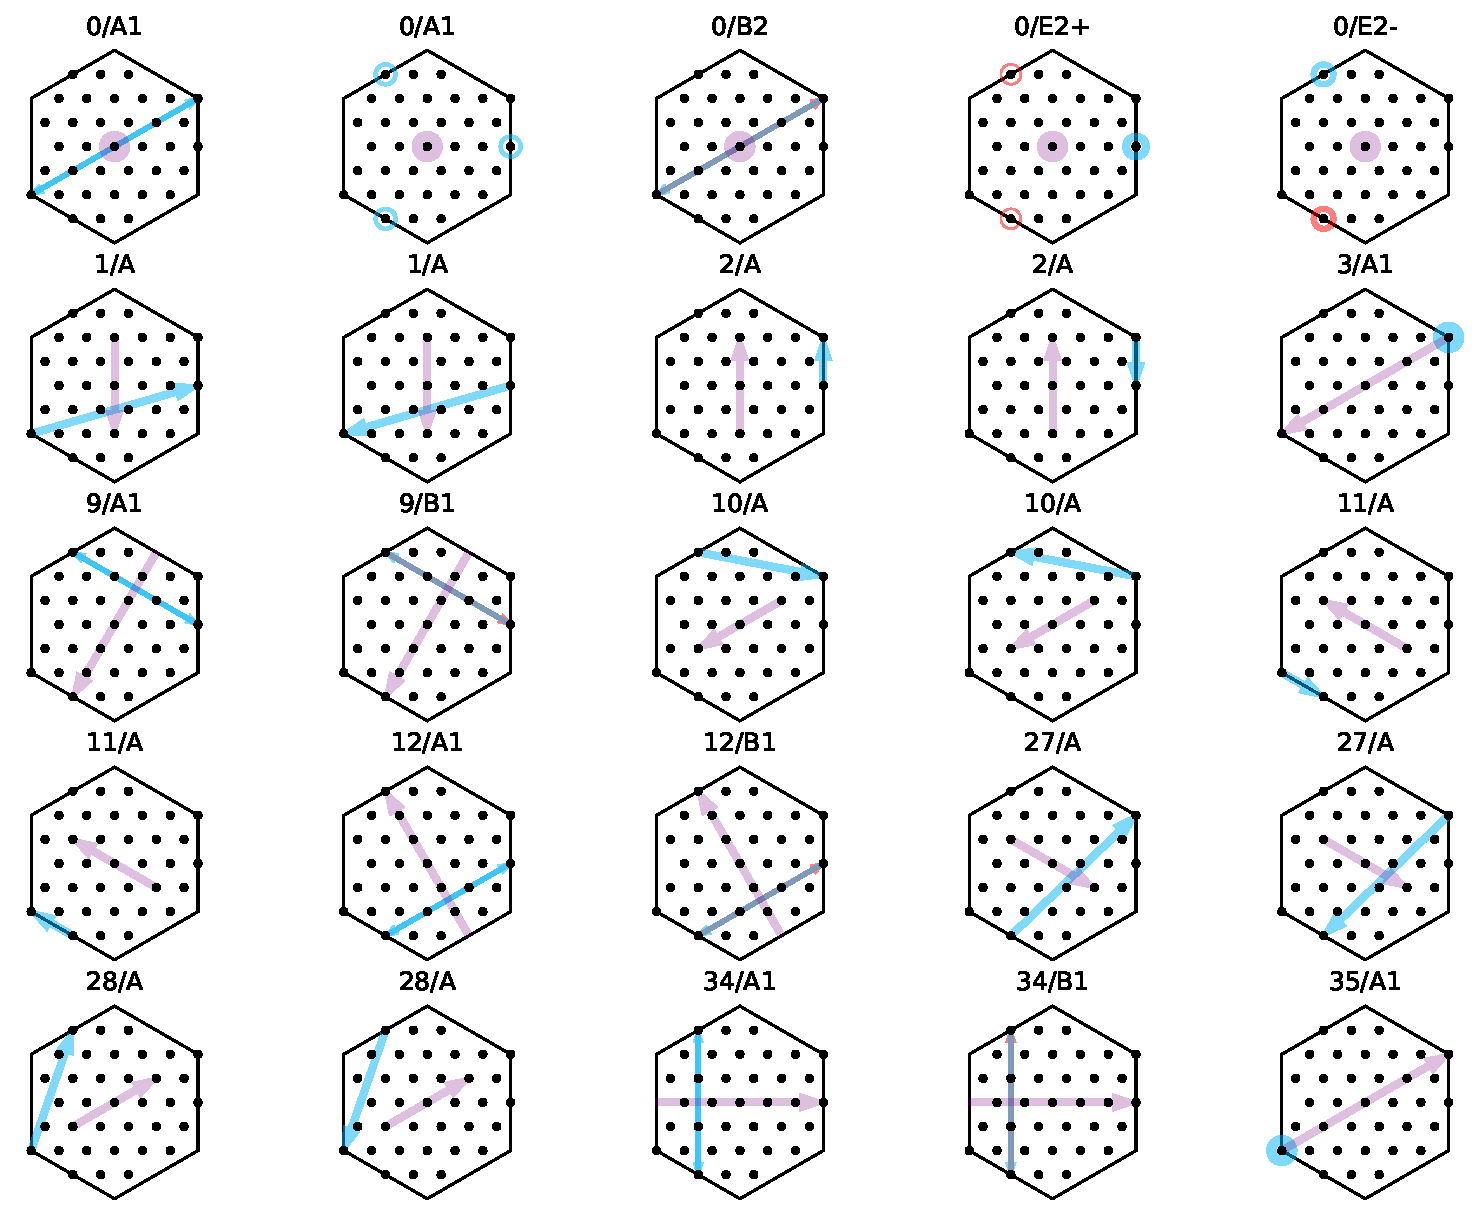
\includegraphics[width=\linewidth]{BZ_KM.pdf}}
    \caption{Example of different momentum shells with their irreducible representations. The number on the left side of "/" in the titles indicates the shell, and on the right side is the irreducible representations of the little group. The head of the pink arrow shows the total momentum $P$; the tail shows $-P$. Only at zero momentum there is a circle. Blue/Red arrows point the relative momentum. The color indicates the phase of the operators (red = $\pi$, blue = 0) and the relative thickness indicates the relative weight of that state.}
    \label{fig:mom_shells}
\end{figure}
We construct total momenta shells with different relative momentum in each one. The transformation of the operators is represented by the little group of $\mathcal{G}$ which preserves the total momentum $\vec{P}$. We can find the irreducible representations for each momentum shell (example \cref{fig:mom_shells}). The momentum labeling of the correlation functions can therefore be changed to
\begin{equation}
  \vec{k},\vec{s} \longrightarrow \vec{P},\vec{p},\rho;
\end{equation}
where $\vec{P} = \vec{k}+\vec{s}$ is the total momentum, $\vec{p} = \frac{\vec{k}-\vec{s}}{2}$ is the relative momentum, and $\rho$ is an irreducible representation of the little group~\cite{evan}.
% Uncomment the following command to get references per chapter.
% Put it inside the file or change \include to \input if you do not want the references
% on a separate page
% \printbibliography[heading=subbibliography]

%------------------------------------------------------------------------------
% Include the following lines and comment out \printbibliography if
% you use BiBTeX for the bibliography.
% If you use biblatex package the files should be specified in the preamble.
% \KOMAoptions{toc=bibliography}
% {\raggedright
%   \bibliographystyle{../refs/atlasBibStyleWithTitle.bst}
%   % \bibliographystyle{unsrt}
%   \bibliography{./thesis_refs,../refs/standard_refs-bibtex}
% }

%------------------------------------------------------------------------------
\appendix
% \part*{Appendix}
% Add your appendices here - don't forget to also add them to \includeonly above
%------------------------------------------------------------------------------
\chapter{Appendix}
\label{sec:app}
%------------------------------------------------------------------------------

\section{Symmetry Correlation Functions}
We will derive in detail how the symmetry operators transform the two-body correlation functions. In this work we are working with only two kinds of correlators, but from them we can also get a feeling of the symmetry transformations. As a side note, it is shown on the right side of the column sign (":") in the titles if the operator transforms well the full Hamiltonian or only at half-filling.

\subsection{Particle-Hole Correlation Function}

Since we have already shown in \cref{ssec:sym-twobody} the transformation of \cref{eq:phhpmat} using the thermal trace cyclicity property, we will directly start from the next symmetry operator.

\subsubsection{\underline{$I : H - \vec{\mu}\cdot\vec{q}$}}

\begin{equation}
  \begin{aligned}
    C_{Q=0,S=1,S^3=-1;k,q,r,s} \\
    =& \frac{1}{Z}tr\left[p_kh_qe^{-H\tau}h^\dagger_rp^\dagger_se^{-H\left(\beta-\tau\right)}\right] \\
    =& \frac{1}{Z}tr\left[I^{-1}Ip_kI^{-1}Ih_qI^{-1}Ie^{-H\tau}I^{-1}Ih^\dagger_rI^{-1}Ip^\dagger_sI^{-1}Ie^{-H\left(\beta-\tau\right)}\right] \\
    =& \frac{1}{Z}tr\left[Ip_kI^{-1}Ih_qI^{-1}Ie^{-H\tau}I^{-1}Ih^\dagger_rI^{-1}Ip^\dagger_sI^{-1}Ie^{-H\left(\beta-\tau\right)I^{-1}}\right] \\
    =& \frac{1}{Z}tr\left[(\Sigma h)^\dagger_k(\Sigma p)^\dagger_qe^{-H\tau}(\Sigma p)_r(\Sigma h)_se^{-H\left(\beta-\tau\right)}\right] \\
    =& \frac{1}{Z}tr\left[(\Sigma p)^\dagger_q(\Sigma h)^\dagger_ke^{-H\tau}(\Sigma h)_s(\Sigma p)_re^{-H\left(\beta-\tau\right)}\right] \\
    =& \frac{1}{Z}tr\left[(\Sigma p)_r(\Sigma h)_se^{-H\left(\beta-\tau\right)}(\Sigma h)^\dagger_k(\Sigma p)^\dagger_qe^{-H\tau}\right]
  \end{aligned}
\end{equation}

\renewcommand{\cor}[4]{p_{#1}h_{#2}h^\dagger_{#3}p^\dagger_{#4}}
\newcommand{\dscor}[4]{\left(\Sigma h\right)_{#1}^\dagger \left(\Sigma p\right)_{#2}^\dagger \left(\Sigma p\right)_{#3}\left(\Sigma h\right)_{#4}}
\renewcommand{\dcor}[4]{h_{#1}^\dagger p_{#2}^\dagger p_{#3} h_{#4}}

\begin{equation}
  \begin{aligned}
    &C_{Q=0,S=1,S^3=-1;k,q,r,s} \\
    &= I^{-1} \left[ 
    {\begin{array}{cccc}
      \cor{+}{+}{+}{+} & \cor{+}{+}{+}{-} & \cor{+}{+}{-}{+} & \cor{+}{+}{-}{-} \\
      \cor{+}{-}{+}{+} & \cor{+}{-}{+}{-} & \cor{+}{-}{-}{+} & \cor{+}{-}{-}{-} \\
      \cor{-}{+}{+}{+} & \cor{-}{+}{+}{-} & \cor{-}{+}{-}{+} & \cor{-}{+}{-}{-} \\
      \cor{-}{-}{+}{+} & \cor{-}{-}{+}{-} & \cor{-}{-}{-}{+} & \cor{-}{-}{-}{-} \\
    \end{array} } \right]_{k,q,r,s} (\tau)\:I \\
    &= \left[\resizebox{\textwidth}{!}{
    ${\begin{array}{cccc}
      \dscor{+}{+}{+}{+} & \dscor{+}{+}{+}{-} & \dscor{+}{+}{-}{+} & \dscor{+}{+}{-}{-} \\
      \dscor{+}{-}{+}{+} & \dscor{+}{-}{+}{-} & \dscor{+}{-}{-}{+} & \dscor{+}{-}{-}{-} \\
      \dscor{-}{+}{+}{+} & \dscor{-}{+}{+}{-} & \dscor{-}{+}{-}{+} & \dscor{-}{+}{-}{-} \\
      \dscor{-}{-}{+}{+} & \dscor{-}{-}{+}{-} & \dscor{-}{-}{-}{+} & \dscor{-}{-}{-}{-} \\
    \end{array} }$}
    \right]_{k,q,r,s} (\tau) \\
    &= \left[ 
    {\begin{array}{cccc}
      \dcor{-}{-}{-}{-} & \dcor{-}{-}{-}{+} & \dcor{-}{-}{+}{-} & \dcor{-}{-}{+}{+} \\
      \dcor{-}{+}{-}{-} & \dcor{-}{+}{-}{+} & \dcor{-}{+}{+}{-} & \dcor{-}{+}{+}{+} \\
      \dcor{+}{-}{-}{-} & \dcor{+}{-}{-}{+} & \dcor{+}{-}{+}{-} & \dcor{+}{-}{+}{+} \\
      \dcor{+}{+}{-}{-} & \dcor{+}{+}{-}{+} & \dcor{+}{+}{+}{-} & \dcor{+}{+}{+}{+} \\
    \end{array} } 
    \right]_{k,q,r,s} (\tau) \\
  \end{aligned}
\end{equation}

\renewcommand{\cor}[4]{p_{#3}h_{#4}h^\dagger_{#1}p^\dagger_{#2}}

\begin{equation}
  \begin{aligned}
    &= \left[ 
    {\begin{array}{cccc}
      \cor{-}{-}{-}{-} & \cor{-}{-}{-}{+} & \cor{-}{-}{+}{-} & \cor{-}{-}{+}{+} \\
      \cor{-}{+}{-}{-} & \cor{-}{+}{-}{+} & \cor{-}{+}{+}{-} & \cor{-}{+}{+}{+} \\
      \cor{+}{-}{-}{-} & \cor{+}{-}{-}{+} & \cor{+}{-}{+}{-} & \cor{+}{-}{+}{+} \\
      \cor{+}{+}{-}{-} & \cor{+}{+}{-}{+} & \cor{+}{+}{+}{-} & \cor{+}{+}{+}{+} \\
    \end{array} } 
    \right]_{r,s,k,q} (\beta-\tau) \\
  \end{aligned}
\end{equation}

\renewcommand{\dcor}[4]{p_{#2}^\dagger h_{#1}^\dagger h_{#4} p_{#3}}

\begin{equation}
  \begin{aligned}
    &= \left[ {\begin{array}{cccc}
      \dcor{-}{-}{-}{-} & \dcor{-}{-}{-}{+} & \dcor{-}{-}{+}{-} & \dcor{-}{-}{+}{+} \\
      \dcor{-}{+}{-}{-} & \dcor{-}{+}{-}{+} & \dcor{-}{+}{+}{-} & \dcor{-}{+}{+}{+} \\
      \dcor{+}{-}{-}{-} & \dcor{+}{-}{-}{+} & \dcor{+}{-}{+}{-} & \dcor{+}{-}{+}{+} \\
      \dcor{+}{+}{-}{-} & \dcor{+}{+}{-}{+} & \dcor{+}{+}{+}{-} & \dcor{+}{+}{+}{+} \\
    \end{array} } \right]_{q,k,s,r} (\tau)
  \end{aligned}
\end{equation}
Depending on what transformation we use to get back to $\langle phh^\dagger p^\dagger\rangle$, we get two transformations which are time reverse to one another. We notice the same behavior for all operators.

\begin{equation}
  \begin{aligned}
    C_{Q=0,S=1,S^3=-1;k,q,r,s} (\tau) \\
    =& \left[ {\begin{array}{cc}
      0 & \sigma_1 \\
      \sigma_1 & 0 \\
    \end{array} } \right]
    {C_{Q=0,S=1,S^3=-1;r,s,k,q}}^\top (\beta-\tau)
    \left[ {\begin{array}{cc}
      0 & \sigma_1 \\
      \sigma_1 & 0 \\
    \end{array} } \right]
  \end{aligned}
\end{equation}

\begin{equation}
  \begin{aligned}
    C_{Q=0,S=1,S^3=-1;k,q,r,s} (\tau) \\
    =& \left[ {\begin{array}{cccc}
      1 & 0 & 0 & 0 \\
      0 & 0 & 1 & 0 \\
      0 & 1 & 0 & 0 \\
      0 & 0 & 0 & 1 \\
    \end{array} } \right]
    \left[ {\begin{array}{cc}
      0 & \sigma_1 \\
      \sigma_1 & 0 \\
    \end{array} } \right]
    C_{Q=0,S=1,S^3=+1;q,k,s,r} (\tau)
    \left[ {\begin{array}{cc}
      0 & \sigma_1 \\
      \sigma_1 & 0 \\
    \end{array} } \right]
    \left[ {\begin{array}{cccc}
      1 & 0 & 0 & 0 \\
      0 & 0 & 1 & 0 \\
      0 & 1 & 0 & 0 \\
      0 & 0 & 0 & 1 \\
    \end{array} } \right]
  \end{aligned}
\end{equation}

\subsubsection{\underline{$C : H$}}

\begin{equation}
  \begin{aligned}
    C_{Q=0,S=1,S^3=-1;k,q,r,s} \\
    =& \frac{1}{Z}tr\left[p_kh_qe^{-H\tau}h^\dagger_rp^\dagger_se^{-H\left(\beta-\tau\right)}\right] \\
    =& \frac{1}{Z}tr\left[C^{-1}Cp_kC^{-1}Ch_qC^{-1}Ce^{-H\tau}C^{-1}Ch^\dagger_rC^{-1}Cp^\dagger_sC^{-1}Ce^{-H\left(\beta-\tau\right)}\right] \\
    =& \frac{1}{Z}tr\left[h_kp_qe^{-H\tau}p^\dagger_rh^\dagger_se^{-H\left(\beta-\tau\right)}\right] \\
    =& \frac{1}{Z}tr\left[p_qh_ke^{-H\tau}h^\dagger_sp^\dagger_re^{-H\left(\beta-\tau\right)}\right]
  \end{aligned}
\end{equation}

\renewcommand{\cor}[4]{p_{#1}h_{#2}h^\dagger_{#3}p^\dagger_{#4}}
\renewcommand{\dcor}[4]{p_{#3}^\dagger h_{#4}^\dagger h_{#1} p_{#2}}

\begin{equation}
  \begin{aligned}
    C_{Q=0,S=1,S^3=-1;k,q,r,s} \\
    &= C^{-1} \left[ 
    {\begin{array}{cccc}
      \cor{+}{+}{+}{+} & \cor{+}{+}{+}{-} & \cor{+}{+}{-}{+} & \cor{+}{+}{-}{-} \\
      \cor{+}{-}{+}{+} & \cor{+}{-}{+}{-} & \cor{+}{-}{-}{+} & \cor{+}{-}{-}{-} \\
      \cor{-}{+}{+}{+} & \cor{-}{+}{+}{-} & \cor{-}{+}{-}{+} & \cor{-}{+}{-}{-} \\
      \cor{-}{-}{+}{+} & \cor{-}{-}{+}{-} & \cor{-}{-}{-}{+} & \cor{-}{-}{-}{-} \\
    \end{array} } \right]_{k,q,r,s} (\tau)\:C \\
  \end{aligned}
\end{equation}

\renewcommand{\cor}[4]{h_{#1}p_{#2}p^\dagger_{#3}h^\dagger_{#4}}

\begin{equation}
  \begin{aligned}  
    &=\left[ {\begin{array}{cccc}
      \cor{+}{+}{+}{+} & \cor{+}{+}{+}{-} & \cor{+}{+}{-}{+} & \cor{+}{+}{-}{-} \\
      \cor{+}{-}{+}{+} & \cor{+}{-}{+}{-} & \cor{+}{-}{-}{+} & \cor{+}{-}{-}{-} \\
      \cor{-}{+}{+}{+} & \cor{-}{+}{+}{-} & \cor{-}{+}{-}{+} & \cor{-}{+}{-}{-} \\
      \cor{-}{-}{+}{+} & \cor{-}{-}{+}{-} & \cor{-}{-}{-}{+} & \cor{-}{-}{-}{-} \\
    \end{array} } \right]_{k,q,r,s} (\tau) \\
    &=\left[ 
    {\begin{array}{cccc}
      \dcor{+}{+}{+}{+} & \dcor{+}{+}{+}{-} & \dcor{+}{+}{-}{+} & \dcor{+}{+}{-}{-} \\
      \dcor{+}{-}{+}{+} & \dcor{+}{-}{+}{-} & \dcor{+}{-}{-}{+} & \dcor{+}{-}{-}{-} \\
      \dcor{-}{+}{+}{+} & \dcor{-}{+}{+}{-} & \dcor{-}{+}{-}{+} & \dcor{-}{+}{-}{-} \\
      \dcor{-}{-}{+}{+} & \dcor{-}{-}{+}{-} & \dcor{-}{-}{-}{+} & \dcor{-}{-}{-}{-} \\
    \end{array} } \right]_{r,s,k,q} (\beta-\tau) \\
  \end{aligned}
\end{equation}

\renewcommand{\cor}[4]{p_{#2}h_{#1}h^\dagger_{#4}p^\dagger_{#3}}

\begin{equation}
  \begin{aligned}
    &=\left[ {\begin{array}{cccc}
      \cor{+}{+}{+}{+} & \cor{+}{+}{+}{-} & \cor{+}{+}{-}{+} & \cor{+}{+}{-}{-} \\
      \cor{+}{-}{+}{+} & \cor{+}{-}{+}{-} & \cor{+}{-}{-}{+} & \cor{+}{-}{-}{-} \\
      \cor{-}{+}{+}{+} & \cor{-}{+}{+}{-} & \cor{-}{+}{-}{+} & \cor{-}{+}{-}{-} \\
      \cor{-}{-}{+}{+} & \cor{-}{-}{+}{-} & \cor{-}{-}{-}{+} & \cor{-}{-}{-}{-} \\
    \end{array} } \right]_{q,k,s,r} (\tau)
  \end{aligned}
\end{equation}

\begin{equation}
  C_{Q=0,S=1,S^3=-1;k,q,r,s} (\tau) = {C_{Q=0,S=1,S^3=+1;r,s,k,q}}^\top (\beta-\tau)
\end{equation}

\begin{equation}
  \begin{aligned}
    C_{Q=0,S=1,S^3=-1;k,q,r,s} (\tau) =
    \left[ {\begin{array}{cccc}
      1 & 0 & 0 & 0 \\
      0 & 0 & 1 & 0 \\
      0 & 1 & 0 & 0 \\
      0 & 0 & 0 & 1 \\
    \end{array} } \right]
    C_{Q=0,S=1,S^3=-1;q,k,s,r}(\tau)
    \left[ {\begin{array}{cccc}
      1 & 0 & 0 & 0 \\
      0 & 0 & 1 & 0 \\
      0 & 1 & 0 & 0 \\
      0 & 0 & 0 & 1 \\
    \end{array} } \right]
  \end{aligned}
\end{equation}

\subsubsection{\underline{$XF : H$}}

\begin{equation}
  \resizebox{\textwidth}{!}{%
  $
  \begin{aligned}
    &C_{Q=0,S=1,S^3=-1;k,q,r,s}\\ 
    &= \frac{1}{Z}tr\left[p_kh_qe^{-H\tau}h^\dagger_rp^\dagger_se^{-H\left(\beta-\tau\right)}\right] \\
    &= \frac{1}{Z}tr\left[(XF)^{-1}(XF)p_k(XF)^{-1}(XF)h_q(XF)^{-1}(XF)e^{-H\tau}(XF)^{-1}(XF)h^\dagger_r(XF)^{-1}(XF)p^\dagger_s(XF)^{-1}(XF)e^{-H\left(\beta-\tau\right)}\right] \\
    &= \frac{1}{Z}tr\left[(\Sigma p)^\dagger_k(\Sigma h)^\dagger_qe^{-H\tau}(\Sigma h)_r(\Sigma p)_se^{-H\left(\beta-\tau\right)}\right]
  \end{aligned}$}
\end{equation}

\renewcommand{\cor}[4]{p_{#1}h_{#2}h^\dagger_{#3}p^\dagger_{#4}}
\renewcommand{\dscor}[4]{\left(\Sigma p\right)_{#1}^\dagger \left(\Sigma h\right)_{#2}^\dagger \left(\Sigma h\right)_{#3}\left(\Sigma p\right)_{#4}}
\renewcommand{\dcor}[4]{p_{#1}^\dagger h_{#2}^\dagger h_{#3} p_{#4}}

\begin{equation}
  \begin{aligned}
    &C_{Q=0,S=1,S^3=-1;k,q,r,s} \\
    &=\left(XF\right)^{-1} \left[ 
    {\begin{array}{cccc}
      \cor{+}{+}{+}{+} & \cor{+}{+}{+}{-} & \cor{+}{+}{-}{+} & \cor{+}{+}{-}{-} \\
      \cor{+}{-}{+}{+} & \cor{+}{-}{+}{-} & \cor{+}{-}{-}{+} & \cor{+}{-}{-}{-} \\
      \cor{-}{+}{+}{+} & \cor{-}{+}{+}{-} & \cor{-}{+}{-}{+} & \cor{-}{+}{-}{-} \\
      \cor{-}{-}{+}{+} & \cor{-}{-}{+}{-} & \cor{-}{-}{-}{+} & \cor{-}{-}{-}{-} \\
    \end{array}}
    \right]_{k,q,r,s} (\tau)\:\left(XF\right) \\
    &= \left[\resizebox{\textwidth}{!}{%
    $
    {\begin{array}{cccc}
      \dscor{+}{+}{+}{+} & \dscor{+}{+}{+}{-} & \dscor{+}{+}{-}{+} & \dscor{+}{+}{-}{-} \\
      \dscor{+}{-}{+}{+} & \dscor{+}{-}{+}{-} & \dscor{+}{-}{-}{+} & \dscor{+}{-}{-}{-} \\
      \dscor{-}{+}{+}{+} & \dscor{-}{+}{+}{-} & \dscor{-}{+}{-}{+} & \dscor{-}{+}{-}{-} \\
      \dscor{-}{-}{+}{+} & \dscor{-}{-}{+}{-} & \dscor{-}{-}{-}{+} & \dscor{-}{-}{-}{-} \\
    \end{array}}$}
    \right]_{k,q,r,s} (\tau) \\
    &= \left[ 
    {\begin{array}{cccc}
      \dcor{-}{-}{-}{-} & \dcor{-}{-}{-}{+} & \dcor{-}{-}{+}{-} & \dcor{-}{-}{+}{+} \\
      \dcor{-}{+}{-}{-} & \dcor{-}{+}{-}{+} & \dcor{-}{+}{+}{-} & \dcor{-}{+}{+}{+} \\
      \dcor{+}{-}{-}{-} & \dcor{+}{-}{-}{+} & \dcor{+}{-}{+}{-} & \dcor{+}{-}{+}{+} \\
      \dcor{+}{+}{-}{-} & \dcor{+}{+}{-}{+} & \dcor{+}{+}{+}{-} & \dcor{+}{+}{+}{+} \\
    \end{array} } \right]_{k,q,r,s} (\tau) \\
  \end{aligned}
\end{equation}
  \renewcommand{\cor}[4]{p_{#4}h_{#3}h^\dagger_{#2}p^\dagger_{#1}}
\begin{equation}
  \begin{aligned}    
    &= \left[ 
    {\begin{array}{cccc}
      \cor{-}{-}{-}{-} & \cor{-}{-}{-}{+} & \cor{-}{-}{+}{-} & \cor{-}{-}{+}{+} \\
      \cor{-}{+}{-}{-} & \cor{-}{+}{-}{+} & \cor{-}{+}{+}{-} & \cor{-}{+}{+}{+} \\
      \cor{+}{-}{-}{-} & \cor{+}{-}{-}{+} & \cor{+}{-}{+}{-} & \cor{+}{-}{+}{+} \\
      \cor{+}{+}{-}{-} & \cor{+}{+}{-}{+} & \cor{+}{+}{+}{-} & \cor{+}{+}{+}{+} \\
    \end{array} } \right]_{s,r,k,q} (\beta-\tau)
  \end{aligned}
\end{equation}

\begin{equation}
  \begin{aligned}
    C_{Q=0,S=1,S^3=-1;k,q,r,s} (\tau) \\
    =& \left[ {\begin{array}{cc}
      0 & \sigma_1 \\
      \sigma_1 & 0 \\
    \end{array} } \right]
    C_{Q=0,S=1,S^3=+1;k,q,r,s} (\tau)
    \left[ {\begin{array}{cc}
      0 & \sigma_1 \\
      \sigma_1 & 0 \\
    \end{array} } \right]
  \end{aligned}
\end{equation}

\begin{equation}
  \begin{aligned}
    C_{Q=0,S=1,S^3=-1;k,q,r,s} (\tau) \\
    =& \left[ {\begin{array}{cccc}
      1 & 0 & 0 & 0 \\
      0 & 0 & 1 & 0 \\
      0 & 1 & 0 & 0 \\
      0 & 0 & 0 & 1 \\
    \end{array} } \right]
    \left[ {\begin{array}{cc}
      0 & \sigma_1 \\
      \sigma_1 & 0 \\
    \end{array} } \right]
    {C_{Q=0,S=1,S^3=-1;s,r,q,k}}^\top (\beta-\tau)
    \left[ {\begin{array}{cc}
      0 & \sigma_1 \\
      \sigma_1 & 0 \\
    \end{array} } \right]
    \left[ {\begin{array}{cccc}
      1 & 0 & 0 & 0 \\
      0 & 0 & 1 & 0 \\
      0 & 1 & 0 & 0 \\
      0 & 0 & 0 & 1 \\
    \end{array} } \right]
  \end{aligned}
\end{equation}

\subsection{Particle-Particle Correlation Function}

The correlation function with two particles at the source and two at the sink can be transformed in more ways. To show this, we start again with correlator $\langle ppp^\dagger p^\dagger\rangle$. In trace and matrix forms it look like this.

\begin{equation}
  C_{Q=2,S=1,S^3=-1;k,q,r,s} = \frac{1}{Z}tr\left[p_kp_qe^{-H\tau}p^\dagger_rp^\dagger_se^{-H\left(\beta-\tau\right)}\right]
\end{equation}

\renewcommand{\cor}[4]{p_{#1}p_{#2}p^\dagger_{#3}p^\dagger_{#4}}
\begin{equation}
  C_{Q=2,S=1,S^3=-1;k,q,r,s} =
  \left[
  \begin{array}{cccc}
    \cor{+}{+}{+}{+} & \cor{+}{+}{+}{-} & \cor{+}{+}{-}{+} & \cor{+}{+}{-}{-} \\
    \cor{+}{-}{+}{+} & \cor{+}{-}{+}{-} & \cor{+}{-}{-}{+} & \cor{+}{-}{-}{-} \\
    \cor{-}{+}{+}{+} & \cor{-}{+}{+}{-} & \cor{-}{+}{-}{+} & \cor{-}{+}{-}{-} \\
    \cor{-}{-}{+}{+} & \cor{-}{-}{+}{-} & \cor{-}{-}{-}{+} & \cor{-}{-}{-}{-} \\
  \end{array}
  \right]_{k,q,r,s} (\tau)
\end{equation}

First, we implement the anti-commutation relations which will give us the identities of this correlation function. Again, we use derive the the results through traces and then continue with the matrix form which will give us a better insight on the transformation of all labels that are included.

\subsubsection{\underline{Anti-commutation}}

\begin{equation}
  \begin{aligned}
    C_{Q=2,S=1,S^3=-1;k,q,r,s} &= \frac{1}{Z}tr\left[p_kp_qe^{-H\tau}p^\dagger_rp^\dagger_se^{-H\left(\beta-\tau\right)}\right] =\\
    &= \frac{1}{Z}tr\left[p_qp_ke^{-H\tau}p^\dagger_sp^\dagger_re^{-H\left(\beta-\tau\right)}\right] \\
    &= - \frac{1}{Z}tr\left[p_qp_ke^{-H\tau}p^\dagger_rp^\dagger_se^{-H\left(\beta-\tau\right)}\right] \\
    &= - \frac{1}{Z}tr\left[p_kp_qe^{-H\tau}p^\dagger_sp^\dagger_re^{-H\left(\beta-\tau\right)}\right]
  \end{aligned}
\end{equation}

% \renewcommand{\cor}[4]{p_{#1}p_{#2}p^\dagger_{#3}p^\dagger_{#4}}
\begin{equation}
  \begin{aligned} 
    C_{Q=2,S=1,S^3=-1;k,q,r,s} &=
    \left[
    \begin{array}{cccc}
      \cor{+}{+}{+}{+} & \cor{+}{+}{+}{-} & \cor{+}{+}{-}{+} & \cor{+}{+}{-}{-} \\
      \cor{+}{-}{+}{+} & \cor{+}{-}{+}{-} & \cor{+}{-}{-}{+} & \cor{+}{-}{-}{-} \\
      \cor{-}{+}{+}{+} & \cor{-}{+}{+}{-} & \cor{-}{+}{-}{+} & \cor{-}{+}{-}{-} \\
      \cor{-}{-}{+}{+} & \cor{-}{-}{+}{-} & \cor{-}{-}{-}{+} & \cor{-}{-}{-}{-} \\
    \end{array}
    \right]_{k,q,r,s} (\tau) \\
    &=\left[ 
    \begin{array}{cccc}
      \cor{+}{+}{+}{+} & \cor{+}{+}{-}{+} & \cor{+}{+}{+}{-} & \cor{+}{+}{-}{-} \\
      \cor{-}{+}{+}{+} & \cor{-}{+}{-}{+} & \cor{-}{+}{+}{-} & \cor{-}{+}{-}{-} \\
      \cor{+}{-}{+}{+} & \cor{+}{-}{-}{+} & \cor{+}{-}{+}{-} & \cor{+}{-}{-}{-} \\
      \cor{-}{-}{+}{+} & \cor{-}{-}{-}{+} & \cor{-}{-}{+}{-} & \cor{-}{-}{-}{-} \\
    \end{array}  
    \right]_{q,k,s,r} (\tau) \\
    &= - \left[
    \begin{array}{cccc}
      \cor{+}{+}{+}{+} & \cor{+}{+}{+}{-} & \cor{+}{+}{-}{+} & \cor{+}{+}{-}{-} \\
      \cor{-}{+}{+}{+} & \cor{-}{+}{+}{-} & \cor{-}{+}{-}{+} & \cor{-}{+}{-}{-} \\
      \cor{+}{-}{+}{+} & \cor{+}{-}{+}{-} & \cor{+}{-}{-}{+} & \cor{+}{-}{-}{-} \\
      \cor{-}{-}{+}{+} & \cor{-}{-}{+}{-} & \cor{-}{-}{-}{+} & \cor{-}{-}{-}{-} \\
    \end{array}
    \right]_{q,k,r,s} (\tau) \\
    &= - \left[
    \begin{array}{cccc}
      \cor{+}{+}{+}{+} & \cor{+}{+}{-}{+} & \cor{+}{+}{+}{-} & \cor{+}{+}{-}{-} \\
      \cor{+}{-}{+}{+} & \cor{+}{-}{-}{+} & \cor{+}{-}{+}{-} & \cor{+}{-}{-}{-} \\
      \cor{-}{+}{+}{+} & \cor{-}{+}{-}{+} & \cor{-}{+}{+}{-} & \cor{-}{+}{-}{-} \\
      \cor{-}{-}{+}{+} & \cor{-}{-}{-}{+} & \cor{-}{-}{+}{-} & \cor{-}{-}{-}{-} \\
    \end{array}
    \right]_{k,q,s,r} (\tau) \\
  \end{aligned}
\end{equation}

\begin{equation}
  \begin{aligned}
    C_{Q=2,S=1,S^3=-1;k,q,r,s} (\tau) &= \sigma_5\cdot C_{Q=2,S=1,S^3=-1;q,k,s,r} (\tau)\cdot\sigma_5\\
    C_{Q=2,S=1,S^3=-1;k,q,r,s} (\tau) &= -\sigma_5\cdot C_{Q=2,S=1,S^3=-1;q,k,s,r} (\tau)\\
    C_{Q=2,S=1,S^3=-1;k,q,r,s} (\tau) &= - C_{Q=2,S=1,S^3=-1;q,k,s,r} (\tau)\cdot\sigma_5
  \end{aligned}
\end{equation}

These identities show us that we can, average our data four fold only because we are using this kind of correlator. Using the cyclicity of the trace, we find how the correlation function transforms when time is reversed. This will further increase our statistics two times.

\subsubsection{\underline{Trace ciclicity}}

\begin{equation}
  \begin{aligned}
    C_{Q=2,S=1,S^3=-1;k,q,r,s} &= \frac{1}{Z}tr\left[p_kp_qe^{-H\tau}p^\dagger_rp^\dagger_se^{-H\left(\beta-\tau\right)}\right] =\\
    &= \frac{1}{Z}tr\left[p^\dagger_rp^\dagger_se^{-H\left(\beta-\tau\right)}p_kp_qe^{-H\tau}\right] \\
    &= \frac{1}{Z}tr\left[p^\dagger_sp^\dagger_re^{-H\left(\beta-\tau\right)}p_qp_ke^{-H\tau}\right] \\
    &= - \frac{1}{Z}tr\left[p^\dagger_sp^\dagger_re^{-H\left(\beta-\tau\right)}p_kp_qe^{-H\tau}\right] \\
    &= - \frac{1}{Z}tr\left[p^\dagger_rp^\dagger_se^{-H\left(\beta-\tau\right)}p_qp_ke^{-H\tau}\right]
  \end{aligned}
\end{equation}

\renewcommand{\dcor}[4]{p^\dagger_{#4}p^\dagger_{#3}p_{#2}p_{#1}}
\begin{equation}
  \begin{aligned} 
    C_{Q=2,S=1,S^3=-1;k,q,r,s} &=
    \left[
    \begin{array}{cccc}
      \cor{+}{+}{+}{+} & \cor{+}{+}{+}{-} & \cor{+}{+}{-}{+} & \cor{+}{+}{-}{-} \\
      \cor{+}{-}{+}{+} & \cor{+}{-}{+}{-} & \cor{+}{-}{-}{+} & \cor{+}{-}{-}{-} \\
      \cor{-}{+}{+}{+} & \cor{-}{+}{+}{-} & \cor{-}{+}{-}{+} & \cor{-}{+}{-}{-} \\
      \cor{-}{-}{+}{+} & \cor{-}{-}{+}{-} & \cor{-}{-}{-}{+} & \cor{-}{-}{-}{-} \\
    \end{array}
    \right]_{k,q,r,s} (\tau) =\\
    &=\left[ 
    \begin{array}{cccc}
      \dcor{+}{+}{+}{+} & \dcor{+}{+}{-}{+} & \dcor{+}{+}{+}{-} & \dcor{+}{+}{-}{-} \\
      \dcor{-}{+}{+}{+} & \dcor{-}{+}{-}{+} & \dcor{-}{+}{+}{-} & \dcor{-}{+}{-}{-} \\
      \dcor{+}{-}{+}{+} & \dcor{+}{-}{-}{+} & \dcor{+}{-}{+}{-} & \dcor{+}{-}{-}{-} \\
      \dcor{-}{-}{+}{+} & \dcor{-}{-}{-}{+} & \dcor{-}{-}{+}{-} & \dcor{-}{-}{-}{-} \\
    \end{array}  
    \right]_{r,s,k,q} (\beta-\tau) \\
    &= \left[
    \begin{array}{cccc}
      \dcor{+}{+}{+}{+} & \dcor{+}{+}{+}{-} & \dcor{+}{+}{-}{+} & \dcor{+}{+}{-}{-} \\
      \dcor{+}{-}{+}{+} & \dcor{+}{-}{+}{-} & \dcor{+}{-}{-}{+} & \dcor{+}{-}{-}{-} \\
      \dcor{-}{+}{+}{+} & \dcor{-}{+}{+}{-} & \dcor{-}{+}{-}{+} & \dcor{-}{+}{-}{-} \\
      \dcor{-}{-}{+}{+} & \dcor{-}{-}{+}{-} & \dcor{-}{-}{-}{+} & \dcor{-}{-}{-}{-} \\
    \end{array}
    \right]_{s,r,q,k} (\beta-\tau) \\
    &= - \left[
    \begin{array}{cccc}
      \dcor{+}{+}{+}{+} & \dcor{+}{+}{+}{-} & \dcor{+}{+}{-}{+} & \dcor{+}{+}{-}{-} \\
      \dcor{-}{+}{+}{+} & \dcor{-}{+}{+}{-} & \dcor{-}{+}{-}{+} & \dcor{-}{+}{-}{-} \\
      \dcor{+}{-}{+}{+} & \dcor{+}{-}{+}{-} & \dcor{+}{-}{-}{+} & \dcor{+}{-}{-}{-} \\
      \dcor{-}{-}{+}{+} & \dcor{-}{-}{+}{-} & \dcor{-}{-}{-}{+} & \dcor{-}{-}{-}{-} \\
    \end{array}
    \right]_{s,r,k,q} (\beta-\tau) \\
    &= - \left[
    \begin{array}{cccc}
      \dcor{+}{+}{+}{+} & \dcor{+}{+}{-}{+} & \dcor{+}{+}{+}{-} & \dcor{+}{+}{-}{-} \\
      \dcor{+}{-}{+}{+} & \dcor{+}{-}{-}{+} & \dcor{+}{-}{+}{-} & \dcor{+}{-}{-}{-} \\
      \dcor{-}{+}{+}{+} & \dcor{-}{+}{-}{+} & \dcor{-}{+}{+}{-} & \dcor{-}{+}{-}{-} \\
      \dcor{-}{-}{+}{+} & \dcor{-}{-}{-}{+} & \dcor{-}{-}{+}{-} & \dcor{-}{-}{-}{-} \\
    \end{array}
    \right]_{r,s,q,k} (\beta-\tau) \\
  \end{aligned}
\end{equation}

\begin{equation}
  \begin{aligned}
    C_{Q=2,S=1,S^3=-1;k,q,r,s} (\tau) &= {C_{Q=2,S=1,S^3=+1;r,s,k,q}}^\top (\beta-\tau) \\
    C_{Q=2,S=1,S^3=-1;k,q,r,s} (\tau) &= \sigma_5\cdot {C_{Q=2,S=1,S^3=+1;s,r,q,k}}^\top (\beta-\tau)\cdot\sigma_5\\
    C_{Q=2,S=1,S^3=-1;k,q,r,s} (\tau) &= - {C_{Q=2,S=1,S^3=+1;s,r,k,q}}^\top (\beta-\tau)\cdot\sigma_5\\
    C_{Q=2,S=1,S^3=-1;k,q,r,s} (\tau) &= - \sigma_5\cdot {C_{Q=2,S=1,S^3=+1;r,s,q,k}}^\top (\beta-\tau)
  \end{aligned}
\end{equation}

\subsubsection{$I : H - \vec{\mu}\cdot\vec{q}$}

\begin{equation}
  \begin{aligned}
    C_{Q=2,S=1,S^3=-1;k,q,r,s} &= \frac{1}{Z}tr\left[p_kp_qe^{-H\tau}p^\dagger_rp^\dagger_se^{-H\left(\beta-\tau\right)}\right] = 
    \\
    &= \frac{1}{Z}tr\left[I^{-1}Ip_kI^{-1}Ip_qI^{-1}Ie^{-H\tau}I^{-1}Ip^\dagger_rI^{-1}Ip^\dagger_sI^{-1}Ie^{-H\left(\beta-\tau\right)}\right] = \\
    &= \frac{1}{Z}tr\left[Ip_kI^{-1}Ip_qI^{-1}Ie^{-H\tau}I^{-1}Ip^\dagger_rI^{-1}Ip^\dagger_sI^{-1}Ie^{-H\left(\beta-\tau\right)}I^{-1}\right] = 
    \\
    &= \frac{1}{Z}tr\left[(\Sigma h)^\dagger_k(\Sigma h)^\dagger_qe^{-H\tau}(\Sigma h)_r(\Sigma h)_se^{-H\left(\beta-\tau\right)}\right] 
    \\
    &= \frac{1}{Z}tr\left[(\Sigma h)^\dagger_q(\Sigma h)^\dagger_ke^{-H\tau}(\Sigma h)_s(\Sigma h)_re^{-H\left(\beta-\tau\right)}\right] 
    \\
    &= - \frac{1}{Z}tr\left[(\Sigma h)^\dagger_q(\Sigma h)^\dagger_ke^{-H\tau}(\Sigma h)_r(\Sigma h)_se^{-H\left(\beta-\tau\right)}\right]
    \\
    &= - \frac{1}{Z}tr\left[(\Sigma h)^\dagger_k(\Sigma h)^\dagger_qe^{-H\tau}(\Sigma h)_s(\Sigma h)_re^{-H\left(\beta-\tau\right)}\right] 
    \\
    &= \frac{1}{Z}tr\left[(\Sigma h)_r(\Sigma h)_se^{-H\left(\beta-\tau\right)}(\Sigma h)^\dagger_k(\Sigma h)^\dagger_qe^{-H\tau}\right] 
    \\
    &= \frac{1}{Z}tr\left[(\Sigma h)_s(\Sigma h)_re^{-H\left(\beta-\tau\right)}(\Sigma h)^\dagger_q(\Sigma h)^\dagger_ke^{-H\tau}\right] 
    \\
    &= - \frac{1}{Z}tr\left[(\Sigma h)_s(\Sigma h)_re^{-H\left(\beta-\tau\right)}(\Sigma h)^\dagger_k(\Sigma h)^\dagger_qe^{-H\tau}\right] 
    \\
    &= - \frac{1}{Z}tr\left[(\Sigma h)_r(\Sigma h)_se^{-H\left(\beta-\tau\right)}(\Sigma h)^\dagger_q(\Sigma h)^\dagger_ke^{-H\tau}\right] 
    \\
  \end{aligned}
\end{equation}

\newcommand{\hdcor}[4]{h^\dagger_{#1}h^\dagger_{#2}h_{#3}h_{#4}}
\newcommand{\hcor}[4]{h_{#3}h_{#4}h^\dagger_{#1}h^\dagger_{#2}}
\renewcommand{\dscor}[4]{\left(\Sigma h\right)_{#1}^\dagger \left(\Sigma h\right)_{#2}^\dagger \left(\Sigma h\right)_{#3}\left(\Sigma h\right)_{#4}}
\begin{equation}
  \begin{aligned} 
    &C_{Q=2,S=1,S^3=-1;k,q,r,s} =
    I^{-1} \left[
    \begin{array}{cccc}
      \cor{+}{+}{+}{+} & \cor{+}{+}{+}{-} & \cor{+}{+}{-}{+} & \cor{+}{+}{-}{-} \\
      \cor{+}{-}{+}{+} & \cor{+}{-}{+}{-} & \cor{+}{-}{-}{+} & \cor{+}{-}{-}{-} \\
      \cor{-}{+}{+}{+} & \cor{-}{+}{+}{-} & \cor{-}{+}{-}{+} & \cor{-}{+}{-}{-} \\
      \cor{-}{-}{+}{+} & \cor{-}{-}{+}{-} & \cor{-}{-}{-}{+} & \cor{-}{-}{-}{-} \\
    \end{array}
    \right]_{k,q,r,s} (\tau) I = \\
    &= \left[\resizebox{\textwidth}{!}{%
    $
    \begin{array}{cccc}
      \dscor{+}{+}{+}{+} & \dscor{+}{+}{+}{-} & \dscor{+}{+}{-}{+} & \dscor{+}{+}{-}{-} \\
      \dscor{+}{-}{+}{+} & \dscor{+}{-}{+}{-} & \dscor{+}{-}{-}{+} & \dscor{+}{-}{-}{-} \\
      \dscor{-}{+}{+}{+} & \dscor{-}{+}{+}{-} & \dscor{-}{+}{-}{+} & \dscor{-}{+}{-}{-} \\
      \dscor{-}{-}{+}{+} & \dscor{-}{-}{+}{-} & \dscor{-}{-}{-}{+} & \dscor{-}{-}{-}{-} \\
    \end{array}$}
    \right]_{k,q,r,s} (\tau) \\
    &= \left[ 
    {\begin{array}{cccc}
      \hdcor{-}{-}{-}{-} & \hdcor{-}{-}{-}{+} & \hdcor{-}{-}{+}{-} & \hdcor{-}{-}{+}{+} \\
      \hdcor{-}{+}{-}{-} & \hdcor{-}{+}{-}{+} & \hdcor{-}{+}{+}{-} & \hdcor{-}{+}{+}{+} \\
      \hdcor{+}{-}{-}{-} & \hdcor{+}{-}{-}{+} & \hdcor{+}{-}{+}{-} & \hdcor{+}{-}{+}{+} \\
      \hdcor{+}{+}{-}{-} & \hdcor{+}{+}{-}{+} & \hdcor{+}{+}{+}{-} & \hdcor{+}{+}{+}{+} \\
    \end{array} } \right]_{k,q,r,s} (\tau) \\
    &= \left[ 
    {\begin{array}{cccc}
      \hdcor{-}{-}{-}{-} & \hdcor{-}{-}{+}{-} & \hdcor{-}{-}{-}{+} & \hdcor{-}{-}{+}{+} \\
      \hdcor{+}{-}{-}{-} & \hdcor{+}{-}{+}{-} & \hdcor{+}{-}{-}{+} & \hdcor{+}{-}{+}{+} \\
      \hdcor{-}{+}{-}{-} & \hdcor{-}{+}{+}{-} & \hdcor{-}{+}{-}{+} & \hdcor{-}{+}{+}{+} \\
      \hdcor{+}{+}{-}{-} & \hdcor{+}{+}{+}{-} & \hdcor{+}{+}{-}{+} & \hdcor{+}{+}{+}{+} \\
    \end{array} } \right]_{q,k,s,r} (\tau) \\
    &= - \left[ 
    {\begin{array}{cccc}
      \hdcor{-}{-}{-}{-} & \hdcor{-}{-}{-}{+} & \hdcor{-}{-}{+}{-} & \hdcor{-}{-}{+}{+} \\
      \hdcor{+}{-}{-}{-} & \hdcor{+}{-}{-}{+} & \hdcor{+}{-}{+}{-} & \hdcor{+}{-}{+}{+} \\
      \hdcor{-}{+}{-}{-} & \hdcor{-}{+}{-}{+} & \hdcor{-}{+}{+}{-} & \hdcor{-}{+}{+}{+} \\
      \hdcor{+}{+}{-}{-} & \hdcor{+}{+}{-}{+} & \hdcor{+}{+}{+}{-} & \hdcor{+}{+}{+}{+} \\
    \end{array} } \right]_{q,k,r,s} (\tau) \\
    &= - \left[ 
    {\begin{array}{cccc}
      \hdcor{-}{-}{-}{-} & \hdcor{-}{-}{+}{-} & \hdcor{-}{-}{-}{+} & \hdcor{-}{-}{+}{+} \\
      \hdcor{-}{+}{-}{-} & \hdcor{-}{+}{+}{-} & \hdcor{-}{+}{-}{+} & \hdcor{-}{+}{+}{+} \\
      \hdcor{+}{-}{-}{-} & \hdcor{+}{-}{+}{-} & \hdcor{+}{-}{-}{+} & \hdcor{+}{-}{+}{+} \\
      \hdcor{+}{+}{-}{-} & \hdcor{+}{+}{+}{-} & \hdcor{+}{+}{-}{+} & \hdcor{+}{+}{+}{+} \\
    \end{array} } \right]_{k,q,s,r} (\tau) \\
    &= \left[ 
    {\begin{array}{cccc}
      \hcor{-}{-}{-}{-} & \hcor{-}{-}{-}{+} & \hcor{-}{-}{+}{-} & \hcor{-}{-}{+}{+} \\
      \hcor{-}{+}{-}{-} & \hcor{-}{+}{-}{+} & \hcor{-}{+}{+}{-} & \hcor{-}{+}{+}{+} \\
      \hcor{+}{-}{-}{-} & \hcor{+}{-}{-}{+} & \hcor{+}{-}{+}{-} & \hcor{+}{-}{+}{+} \\
      \hcor{+}{+}{-}{-} & \hcor{+}{+}{-}{+} & \hcor{+}{+}{+}{-} & \hcor{+}{+}{+}{+} \\
    \end{array} } \right]_{r,s,k,q} (\beta-\tau) \\
    &= \left[ 
    {\begin{array}{cccc}
      \hcor{-}{-}{-}{-} & \hcor{-}{-}{+}{-} & \hcor{-}{-}{-}{+} & \hcor{-}{-}{+}{+} \\
      \hcor{+}{-}{-}{-} & \hcor{+}{-}{+}{-} & \hcor{+}{-}{-}{+} & \hcor{+}{-}{+}{+} \\
      \hcor{-}{+}{-}{-} & \hcor{-}{+}{+}{-} & \hcor{-}{+}{-}{+} & \hcor{-}{+}{+}{+} \\
      \hcor{+}{+}{-}{-} & \hcor{+}{+}{+}{-} & \hcor{+}{+}{-}{+} & \hcor{+}{+}{+}{+} \\
    \end{array} } \right]_{s,r,q,k} (\beta-\tau) \\
    &= - \left[ 
    {\begin{array}{cccc}
      \hcor{-}{-}{-}{-} & \hcor{-}{-}{+}{-} & \hcor{-}{-}{-}{+} & \hcor{-}{-}{+}{+} \\
      \hcor{-}{+}{-}{-} & \hcor{-}{+}{+}{-} & \hcor{-}{+}{-}{+} & \hcor{-}{+}{+}{+} \\
      \hcor{+}{-}{-}{-} & \hcor{+}{-}{+}{-} & \hcor{+}{-}{-}{+} & \hcor{+}{-}{+}{+} \\
      \hcor{+}{+}{-}{-} & \hcor{+}{+}{+}{-} & \hcor{+}{+}{-}{+} & \hcor{+}{+}{+}{+} \\
    \end{array} } \right]_{s,r,k,q} (\beta-\tau) \\
    &= - \left[ 
    {\begin{array}{cccc}
      \hcor{-}{-}{-}{-} & \hcor{-}{-}{-}{+} & \hcor{-}{-}{+}{-} & \hcor{-}{-}{+}{+} \\
      \hcor{+}{-}{-}{-} & \hcor{+}{-}{-}{+} & \hcor{+}{-}{+}{-} & \hcor{+}{-}{+}{+} \\
      \hcor{-}{+}{-}{-} & \hcor{-}{+}{-}{+} & \hcor{-}{+}{+}{-} & \hcor{-}{+}{+}{+} \\
      \hcor{+}{+}{-}{-} & \hcor{+}{+}{-}{+} & \hcor{+}{+}{+}{-} & \hcor{+}{+}{+}{+} \\
    \end{array} } \right]_{r,s,q,k} (\beta-\tau) \\
  \end{aligned}
\end{equation}

\begin{equation}
  \begin{aligned}
    C_{Q=2,S=1,S^3=-1;k,q,r,s} (\tau) &= \sigma_1\cdot{C_{Q=-2,S=1,S^3=+1;k,q,r,s}} (\tau)\cdot\sigma_1 
    \\
    C_{Q=2,S=1,S^3=-1;k,q,r,s} (\tau) &= \sigma_5\cdot \sigma_1\cdot{C_{Q=-2,S=1,S^3=+1;q,k,s,r}} (\tau)\cdot\sigma_1\cdot\sigma_5
    \\
    C_{Q=2,S=1,S^3=-1;k,q,r,s} (\tau) &= - \sigma_5\cdot \sigma_1\cdot{C_{Q=-2,S=1,S^3=+1;q,k,r,s}} (\tau)\cdot\sigma_1
    \\
    C_{Q=2,S=1,S^3=-1;k,q,r,s} (\tau) &= - \sigma_1\cdot{C_{Q=-2,S=1,S^3=+1;k,q,s,r}} (\tau)\cdot\sigma_1\cdot\sigma_5
    \\
    C_{Q=2,S=1,S^3=-1;k,q,r,s} (\tau) &= \sigma_1\cdot{C_{Q=-2,S=1,S^3=-1;r,s,k,q}}^\top (\beta-\tau) \cdot\sigma_1 
    \\
    C_{Q=2,S=1,S^3=-1;k,q,r,s} (\tau) &= \sigma_5\cdot \sigma_1\cdot{C_{Q=-2,S=1,S^3=-1;s,r,q,k}}^\top (\beta-\tau) \cdot\sigma_1\cdot\sigma_5
    \\
    C_{Q=2,S=1,S^3=-1;k,q,r,s} (\tau) &= - \sigma_1\cdot{C_{Q=-2,S=1,S^3=-1;s,r,k,q}}^\top (\beta-\tau) \cdot\sigma_1\cdot\sigma_5
    \\
    C_{Q=2,S=1,S^3=-1;k,q,r,s} (\tau) &= - \sigma_5\cdot \sigma_1\cdot{C_{Q=-2,S=1,S^3=-1;r,s,q,k}}^\top (\beta-\tau) \cdot\sigma_1
    \\
  \end{aligned}
\end{equation}

\subsubsection{$C : H$}

\begin{equation}
  \begin{aligned}
    C_{Q=2,S=1,S^3=-1;k,q,r,s} &= \frac{1}{Z}tr\left[p_kp_qe^{-H\tau}p^\dagger_rp^\dagger_se^{-H\left(\beta-\tau\right)}\right] = 
    \\
    &= \frac{1}{Z}tr\left[C^{-1}Cp_kC^{-1}Cp_qC^{-1}Ce^{-H\tau}C^{-1}Cp^\dagger_rC^{-1}Cp^\dagger_sC^{-1}Ce^{-H\left(\beta-\tau\right)}\right] = 
    \\
    &= \frac{1}{Z}tr\left[Cp_kC^{-1}Cp_qC^{-1}Ce^{-H\tau}C^{-1}Cp^\dagger_rC^{-1}Cp^\dagger_sC^{-1}Ce^{-H\left(\beta-\tau\right)}C^{-1}\right] = 
    \\
    &= \frac{1}{Z}tr\left[h_kh_qe^{-H\tau}h^\dagger_rh^\dagger_se^{-H\left(\beta-\tau\right)}\right]
    \\
    &= \frac{1}{Z}tr\left[h_qh_k{-H\tau}h^\dagger_sh^\dagger_re^{-H\left(\beta-\tau\right)}\right]
    \\
    &= - \frac{1}{Z}tr\left[h_qh_ke^{-H\tau}h^\dagger_rh^\dagger_se^{-H\left(\beta-\tau\right)}\right]
    \\
    &= - \frac{1}{Z}tr\left[h_kh_qe^{-H\tau}h^\dagger_sh^\dagger_re^{-H\left(\beta-\tau\right)}\right]
    \\
    &= \frac{1}{Z}tr\left[h^\dagger_rh^\dagger_se^{-H\left(\beta-\tau\right)}h_kh_qe^{-H\tau}\right]
    \\
    &= \frac{1}{Z}tr\left[h^\dagger_sh^\dagger_re^{-H\left(\beta-\tau\right)}h_qh_ke^{-H\tau}\right]
    \\
    &= - \frac{1}{Z}tr\left[h^\dagger_sh^\dagger_re^{-H\left(\beta-\tau\right)}h_kh_qe^{-H\tau}\right]
    \\
    &= - \frac{1}{Z}tr\left[h^\dagger_rh^\dagger_se^{-H\left(\beta-\tau\right)}h_qh_ke^{-H\tau}\right]
    \\
  \end{aligned}
\end{equation}

\renewcommand{\hcor}[4]{h_{#1}h_{#2}h^\dagger_{#3}h^\dagger_{#4}}
\renewcommand{\hdcor}[4]{h^\dagger_{#4}h^\dagger_{#3}h_{#2}h_{#1}}
\begin{equation}
  \begin{aligned} 
    &C_{Q=2,S=1,S^3=-1;k,q,r,s} =
    C^{-1} \left[
    \begin{array}{cccc}
      \cor{+}{+}{+}{+} & \cor{+}{+}{+}{-} & \cor{+}{+}{-}{+} & \cor{+}{+}{-}{-} \\
      \cor{+}{-}{+}{+} & \cor{+}{-}{+}{-} & \cor{+}{-}{-}{+} & \cor{+}{-}{-}{-} \\
      \cor{-}{+}{+}{+} & \cor{-}{+}{+}{-} & \cor{-}{+}{-}{+} & \cor{-}{+}{-}{-} \\
      \cor{-}{-}{+}{+} & \cor{-}{-}{+}{-} & \cor{-}{-}{-}{+} & \cor{-}{-}{-}{-} \\
    \end{array}
    \right]_{k,q,r,s} (\tau) C = \\
    &= \left[ 
    {\begin{array}{cccc}
      \hcor{+}{+}{+}{+} & \hcor{+}{+}{+}{-} & \hcor{+}{+}{-}{+} & \hcor{+}{+}{-}{-} \\
      \hcor{+}{-}{+}{+} & \hcor{+}{-}{+}{-} & \hcor{+}{-}{-}{+} & \hcor{+}{-}{-}{-} \\
      \hcor{-}{+}{+}{+} & \hcor{-}{+}{+}{-} & \hcor{-}{+}{-}{+} & \hcor{-}{+}{-}{-} \\
      \hcor{-}{-}{+}{+} & \hcor{-}{-}{+}{-} & \hcor{-}{-}{-}{+} & \hcor{-}{-}{-}{-} \\
    \end{array} } \right]_{k,q,r,s} (\tau) \\
    &= \left[ 
    {\begin{array}{cccc}
      \hcor{+}{+}{+}{+} & \hcor{+}{+}{-}{+} & \hcor{+}{+}{+}{-} & \hcor{+}{+}{-}{-} \\
      \hcor{-}{+}{+}{+} & \hcor{-}{+}{-}{+} & \hcor{-}{+}{+}{-} & \hcor{-}{+}{-}{-} \\
      \hcor{+}{-}{+}{+} & \hcor{+}{-}{-}{+} & \hcor{+}{-}{+}{-} & \hcor{+}{-}{-}{-} \\
      \hcor{-}{-}{+}{+} & \hcor{-}{-}{-}{+} & \hcor{-}{-}{+}{-} & \hcor{-}{-}{-}{-} \\
    \end{array} } \right]_{q,k,s,r} (\tau) \\
    &= - \left[ 
    {\begin{array}{cccc}
      \hcor{+}{+}{+}{+} & \hcor{+}{+}{+}{-} & \hcor{+}{+}{-}{+} & \hcor{+}{+}{-}{-} \\
      \hcor{-}{+}{+}{+} & \hcor{-}{+}{+}{-} & \hcor{-}{+}{-}{+} & \hcor{-}{+}{-}{-} \\
      \hcor{+}{-}{+}{+} & \hcor{+}{-}{+}{-} & \hcor{+}{-}{-}{+} & \hcor{+}{-}{-}{-} \\
      \hcor{-}{-}{+}{+} & \hcor{-}{-}{+}{-} & \hcor{-}{-}{-}{+} & \hcor{-}{-}{-}{-} \\
    \end{array} } \right]_{q,k,r,s} (\tau) \\
    &= - \left[ 
    {\begin{array}{cccc}
      \hdcor{+}{+}{+}{+} & \hdcor{+}{+}{-}{+} & \hdcor{+}{+}{+}{-} & \hdcor{+}{+}{-}{-} \\
      \hdcor{+}{-}{+}{+} & \hdcor{+}{-}{-}{+} & \hdcor{+}{-}{+}{-} & \hdcor{+}{-}{-}{-} \\
      \hdcor{-}{+}{+}{+} & \hdcor{-}{+}{-}{+} & \hdcor{-}{+}{+}{-} & \hdcor{-}{+}{-}{-} \\
      \hdcor{-}{-}{+}{+} & \hdcor{-}{-}{-}{+} & \hdcor{-}{-}{+}{-} & \hdcor{-}{-}{-}{-} \\
    \end{array} } \right]_{k,q,s,r} (\tau) \\
    &= \left[ 
    {\begin{array}{cccc}
      \hdcor{+}{+}{+}{+} & \hdcor{+}{+}{-}{+} & \hdcor{+}{+}{+}{-} & \hdcor{+}{+}{-}{-} \\
      \hdcor{-}{+}{+}{+} & \hdcor{-}{+}{-}{+} & \hdcor{-}{+}{+}{-} & \hdcor{-}{+}{-}{-} \\
      \hdcor{+}{-}{+}{+} & \hdcor{+}{-}{-}{+} & \hdcor{+}{-}{+}{-} & \hdcor{+}{-}{-}{-} \\
      \hdcor{-}{-}{+}{+} & \hdcor{-}{-}{-}{+} & \hdcor{-}{-}{+}{-} & \hdcor{-}{-}{-}{-} \\
    \end{array} } \right]_{r,s,k,q} (\beta-\tau) \\
    &= \left[ 
    {\begin{array}{cccc}
      \hdcor{+}{+}{+}{+} & \hdcor{+}{+}{+}{-} & \hdcor{+}{+}{-}{+} & \hdcor{+}{+}{-}{-} \\
      \hdcor{+}{-}{+}{+} & \hdcor{+}{-}{+}{-} & \hdcor{+}{-}{-}{+} & \hdcor{+}{-}{-}{-} \\
      \hdcor{-}{+}{+}{+} & \hdcor{-}{+}{+}{-} & \hdcor{-}{+}{-}{+} & \hdcor{-}{+}{-}{-} \\
      \hdcor{-}{-}{+}{+} & \hdcor{-}{-}{+}{-} & \hdcor{-}{-}{-}{+} & \hdcor{-}{-}{-}{-} \\
    \end{array} } \right]_{s,r,q,k} (\beta-\tau) \\
    &= - \left[ 
    {\begin{array}{cccc}
      \hdcor{+}{+}{+}{+} & \hdcor{+}{+}{+}{-} & \hdcor{+}{+}{-}{+} & \hdcor{+}{+}{-}{-} \\
      \hdcor{-}{+}{+}{+} & \hdcor{-}{+}{+}{-} & \hdcor{-}{+}{-}{+} & \hdcor{-}{+}{-}{-} \\
      \hdcor{+}{-}{+}{+} & \hdcor{+}{-}{+}{-} & \hdcor{+}{-}{-}{+} & \hdcor{+}{-}{-}{-} \\
      \hdcor{-}{-}{+}{+} & \hdcor{-}{-}{+}{-} & \hdcor{-}{-}{-}{+} & \hdcor{-}{-}{-}{-} \\
    \end{array} } \right]_{s,r,k,q} (\beta-\tau) \\
    &= - \left[ 
    {\begin{array}{cccc}
      \hdcor{+}{+}{+}{+} & \hdcor{+}{+}{-}{+} & \hdcor{+}{+}{+}{-} & \hdcor{+}{+}{-}{-} \\
      \hdcor{+}{-}{+}{+} & \hdcor{+}{-}{-}{+} & \hdcor{+}{-}{+}{-} & \hdcor{+}{-}{-}{-} \\
      \hdcor{-}{+}{+}{+} & \hdcor{-}{+}{-}{+} & \hdcor{-}{+}{+}{-} & \hdcor{-}{+}{-}{-} \\
      \hdcor{-}{-}{+}{+} & \hdcor{-}{-}{-}{+} & \hdcor{-}{-}{+}{-} & \hdcor{-}{-}{-}{-} \\
    \end{array} } \right]_{r,s,q,k} (\beta-\tau) \\
  \end{aligned}
\end{equation}

\begin{equation}
  \begin{aligned}
    C_{Q=2,S=1,S^3=-1;k,q,r,s} (\tau) &= {C_{Q=-2,S=1,S^3=-1;k,q,r,s}} (\tau) 
    \\
    C_{Q=2,S=1,S^3=-1;k,q,r,s} (\tau) &= \sigma_5\cdot {C_{Q=-2,S=1,S^3=-1;q,k,s,r}} (\tau)\cdot\sigma_5
    \\
    C_{Q=2,S=1,S^3=-1;k,q,r,s} (\tau) &= - \sigma_5\cdot {C_{Q=-2,S=1,S^3=-1;q,k,r,s}} (\tau)
    \\
    C_{Q=2,S=1,S^3=-1;k,q,r,s} (\tau) &= - {C_{Q=-2,S=1,S^3=-1;k,q,s,r}} (\tau)\cdot\sigma_5
    \\
    C_{Q=2,S=1,S^3=-1;k,q,r,s} (\tau) &= {C_{Q=-2,S=1,S^3=+1;r,s,k,q}}^\top (\beta-\tau) 
    \\
    C_{Q=2,S=1,S^3=-1;k,q,r,s} (\tau) &= \sigma_5\cdot {C_{Q=-2,S=1,S^3=+1;s,r,q,k}}^\top (\beta-\tau)\cdot\sigma_5
    \\
    C_{Q=2,S=1,S^3=-1;k,q,r,s} (\tau) &= - {C_{Q=-2,S=1,S^3=+1;s,r,k,q}}^\top (\beta-\tau)\cdot\sigma_5
    \\
    C_{Q=2,S=1,S^3=-1;k,q,r,s} (\tau) &= - \sigma_5\cdot {C_{Q=-2,S=1,S^3=+1;r,s,q,k}}^\top (\beta-\tau)
    \\
  \end{aligned}
\end{equation}

\subsubsection{$XF : H$}

\begin{equation}
  \resizebox{\textwidth}{!}{%
  $
  \begin{aligned}
    &C_{Q=2,S=1,S^3=-1;k,q,r,s} = \frac{1}{Z}tr\left[p_kp_qe^{-H\tau}p^\dagger_rp^\dagger_se^{-H\left(\beta-\tau\right)}\right] = 
    \\
    &= \frac{1}{Z}tr\left[(XF)^{-1}(XF)p_k(XF)^{-1}(XF)p_q(XF)^{-1}(XF)e^{-H\tau}(XF)^{-1}(XF)p^\dagger_r(XF)^{-1}(XF)p^\dagger_s(XF)^{-1}(XF)e^{-H\left(\beta-\tau\right)}\right] = 
    \\
    &= \frac{1}{Z}tr\left[(XF)p_k(XF)^{-1}(XF)p_q(XF)^{-1}(XF)e^{-H\tau}(XF)^{-1}(XF)p^\dagger_r(XF)^{-1}(XF)p^\dagger_s(XF)^{-1}(XF)e^{-H\left(\beta-\tau\right)}(XF)^{-1}\right] = 
    \\
    &= \frac{1}{Z}tr\left[(\Sigma p)^\dagger_k(\Sigma p)^\dagger_qe^{-H\tau}(\Sigma p)_r(\Sigma p)_se^{-H\left(\beta-\tau\right)}\right]
    \\
    &= \frac{1}{Z}tr\left[(\Sigma p)^\dagger_q(\Sigma p)^\dagger_ke^{-H\tau}(\Sigma p)_s(\Sigma p)_re^{-H\left(\beta-\tau\right)}\right]
    \\
    &= - \frac{1}{Z}tr\left[(\Sigma p)^\dagger_q(\Sigma p)^\dagger_ke^{-H\tau}(\Sigma p)_r(\Sigma p)_se^{-H\left(\beta-\tau\right)}\right]
    \\
    &= - \frac{1}{Z}tr\left[(\Sigma p)^\dagger_k(\Sigma p)^\dagger_qe^{-H\tau}(\Sigma p)_s(\Sigma p)_re^{-H\left(\beta-\tau\right)}\right]
    \\
    &= \frac{1}{Z}tr\left[(\Sigma p)_r(\Sigma p)_se^{-H\left(\beta-\tau\right)}(\Sigma p)^\dagger_k(\Sigma p)^\dagger_qe^{-H\tau}\right]
    \\
    &= \frac{1}{Z}tr\left[(\Sigma p)_s(\Sigma p)_re^{-H\left(\beta-\tau\right)}(\Sigma p)^\dagger_q(\Sigma p)^\dagger_ke^{-H\tau}\right]
    \\
    &= - \frac{1}{Z}tr\left[(\Sigma p)_s(\Sigma p)_re^{-H\left(\beta-\tau\right)}(\Sigma p)^\dagger_k(\Sigma p)^\dagger_qe^{-H\tau}\right]
    \\
    &= - \frac{1}{Z}tr\left[(\Sigma p)_r(\Sigma p)_se^{-H\left(\beta-\tau\right)}(\Sigma p)^\dagger_q(\Sigma p)^\dagger_ke^{-H\tau}\right]
    \\
  \end{aligned}$}
\end{equation}

\renewcommand{\dscor}[4]{\left(\Sigma p\right)_{#1}^\dagger \left(\Sigma p\right)_{#2}^\dagger \left(\Sigma p\right)_{#3}\left(\Sigma p\right)_{#4}}
\renewcommand{\dcor}[4]{p^\dagger_{#1}p^\dagger_{#2}p_{#3}p_{#4}}
\newcommand{\rcor}[4]{p_{#3}p_{#4}p^\dagger_{#1}p^\dagger_{#2}}
\begin{equation}
  \begin{aligned} 
    &C_{Q=2,S=1,S^3=-1;k,q,r,s} =
    (XF)^{-1} \left[
    \begin{array}{cccc}
      \cor{+}{+}{+}{+} & \cor{+}{+}{+}{-} & \cor{+}{+}{-}{+} & \cor{+}{+}{-}{-} \\
      \cor{+}{-}{+}{+} & \cor{+}{-}{+}{-} & \cor{+}{-}{-}{+} & \cor{+}{-}{-}{-} \\
      \cor{-}{+}{+}{+} & \cor{-}{+}{+}{-} & \cor{-}{+}{-}{+} & \cor{-}{+}{-}{-} \\
      \cor{-}{-}{+}{+} & \cor{-}{-}{+}{-} & \cor{-}{-}{-}{+} & \cor{-}{-}{-}{-} \\
    \end{array}
    \right]_{k,q,r,s} (\tau) (XF) = \\
    &= \left[\resizebox{\textwidth}{!}{%
    $
    \begin{array}{cccc}
      \dscor{+}{+}{+}{+} & \dscor{+}{+}{+}{-} & \dscor{+}{+}{-}{+} & \dscor{+}{+}{-}{-} \\
      \dscor{+}{-}{+}{+} & \dscor{+}{-}{+}{-} & \dscor{+}{-}{-}{+} & \dscor{+}{-}{-}{-} \\
      \dscor{-}{+}{+}{+} & \dscor{-}{+}{+}{-} & \dscor{-}{+}{-}{+} & \dscor{-}{+}{-}{-} \\
      \dscor{-}{-}{+}{+} & \dscor{-}{-}{+}{-} & \dscor{-}{-}{-}{+} & \dscor{-}{-}{-}{-} \\
    \end{array}$}
    \right]_{k,q,r,s} (\tau) \\
    &= \left[ 
    {\begin{array}{cccc}
      \dcor{-}{-}{-}{-} & \dcor{-}{-}{-}{+} & \dcor{-}{-}{+}{-} & \dcor{-}{-}{+}{+} \\
      \dcor{-}{+}{-}{-} & \dcor{-}{+}{-}{+} & \dcor{-}{+}{+}{-} & \dcor{-}{+}{+}{+} \\
      \dcor{+}{-}{-}{-} & \dcor{+}{-}{-}{+} & \dcor{+}{-}{+}{-} & \dcor{+}{-}{+}{+} \\
      \dcor{+}{+}{-}{-} & \dcor{+}{+}{-}{+} & \dcor{+}{+}{+}{-} & \dcor{+}{+}{+}{+} \\
    \end{array} } \right]_{k,q,r,s} (\tau) \\
    &= \left[ 
    {\begin{array}{cccc}
      \dcor{-}{-}{-}{-} & \dcor{-}{-}{+}{-} & \dcor{-}{-}{-}{+} & \dcor{-}{-}{+}{+} \\
      \dcor{+}{-}{-}{-} & \dcor{+}{-}{+}{-} & \dcor{+}{-}{-}{+} & \dcor{+}{-}{+}{+} \\
      \dcor{-}{+}{-}{-} & \dcor{-}{+}{+}{-} & \dcor{-}{+}{-}{+} & \dcor{-}{+}{+}{+} \\
      \dcor{+}{+}{-}{-} & \dcor{+}{+}{+}{-} & \dcor{+}{+}{-}{+} & \dcor{+}{+}{+}{+} \\
    \end{array} } \right]_{q,k,s,r} (\tau) \\
    &= - \left[ 
    {\begin{array}{cccc}
      \dcor{-}{-}{-}{-} & \dcor{-}{-}{-}{+} & \dcor{-}{-}{+}{-} & \dcor{-}{-}{+}{+} \\
      \dcor{+}{-}{-}{-} & \dcor{+}{-}{-}{+} & \dcor{+}{-}{+}{-} & \dcor{+}{-}{+}{+} \\
      \dcor{-}{+}{-}{-} & \dcor{-}{+}{-}{+} & \dcor{-}{+}{+}{-} & \dcor{-}{+}{+}{+} \\
      \dcor{+}{+}{-}{-} & \dcor{+}{+}{-}{+} & \dcor{+}{+}{+}{-} & \dcor{+}{+}{+}{+} \\
    \end{array} } \right]_{q,k,r,s} (\tau) \\
    &= - \left[ 
    {\begin{array}{cccc}
      \dcor{-}{-}{-}{-} & \dcor{-}{-}{+}{-} & \dcor{-}{-}{-}{+} & \dcor{-}{-}{+}{+} \\
      \dcor{-}{+}{-}{-} & \dcor{-}{+}{+}{-} & \dcor{-}{+}{-}{+} & \dcor{-}{+}{+}{+} \\
      \dcor{+}{-}{-}{-} & \dcor{+}{-}{+}{-} & \dcor{+}{-}{-}{+} & \dcor{+}{-}{+}{+} \\
      \dcor{+}{+}{-}{-} & \dcor{+}{+}{+}{-} & \dcor{+}{+}{-}{+} & \dcor{+}{+}{+}{+} \\
    \end{array} } \right]_{k,q,s,r} (\tau) \\
    &= \left[ 
    {\begin{array}{cccc}
      \rcor{-}{-}{-}{-} & \rcor{-}{-}{-}{+} & \rcor{-}{-}{+}{-} & \rcor{-}{-}{+}{+} \\
      \rcor{-}{+}{-}{-} & \rcor{-}{+}{-}{+} & \rcor{-}{+}{+}{-} & \rcor{-}{+}{+}{+} \\
      \rcor{+}{-}{-}{-} & \rcor{+}{-}{-}{+} & \rcor{+}{-}{+}{-} & \rcor{+}{-}{+}{+} \\
      \rcor{+}{+}{-}{-} & \rcor{+}{+}{-}{+} & \rcor{+}{+}{+}{-} & \rcor{+}{+}{+}{+} \\
    \end{array} } \right]_{r,s,k,q} (\beta-\tau) \\
    &= \left[ 
    {\begin{array}{cccc}
      \rcor{-}{-}{-}{-} & \rcor{-}{-}{+}{-} & \rcor{-}{-}{-}{+} & \rcor{-}{-}{+}{+} \\
      \rcor{+}{-}{-}{-} & \rcor{+}{-}{+}{-} & \rcor{+}{-}{-}{+} & \rcor{+}{-}{+}{+} \\
      \rcor{-}{+}{-}{-} & \rcor{-}{+}{+}{-} & \rcor{-}{+}{-}{+} & \rcor{-}{+}{+}{+} \\
      \rcor{+}{+}{-}{-} & \rcor{+}{+}{+}{-} & \rcor{+}{+}{-}{+} & \rcor{+}{+}{+}{+} \\
    \end{array} } \right]_{s,r,q,k} (\beta-\tau) \\
    &= - \left[ 
    {\begin{array}{cccc}
      \rcor{-}{-}{-}{-} & \rcor{-}{-}{+}{-} & \rcor{-}{-}{-}{+} & \rcor{-}{-}{+}{+} \\
      \rcor{-}{+}{-}{-} & \rcor{-}{+}{+}{-} & \rcor{-}{+}{-}{+} & \rcor{-}{+}{+}{+} \\
      \rcor{+}{-}{-}{-} & \rcor{+}{-}{+}{-} & \rcor{+}{-}{-}{+} & \rcor{+}{-}{+}{+} \\
      \rcor{+}{+}{-}{-} & \rcor{+}{+}{+}{-} & \rcor{+}{+}{-}{+} & \rcor{+}{+}{+}{+} \\
    \end{array} } \right]_{s,r,k,q} (\beta-\tau) \\ 
    &= - \left[ 
    {\begin{array}{cccc}
      \rcor{-}{-}{-}{-} & \rcor{-}{-}{-}{+} & \rcor{-}{-}{+}{-} & \rcor{-}{-}{+}{+} \\
      \rcor{+}{-}{-}{-} & \rcor{+}{-}{-}{+} & \rcor{+}{-}{+}{-} & \rcor{+}{-}{+}{+} \\
      \rcor{-}{+}{-}{-} & \rcor{-}{+}{-}{+} & \rcor{-}{+}{+}{-} & \rcor{-}{+}{+}{+} \\
      \rcor{+}{+}{-}{-} & \rcor{+}{+}{-}{+} & \rcor{+}{+}{+}{-} & \rcor{+}{+}{+}{+} \\
    \end{array} } \right]_{r,s,q,k} (\beta-\tau) \\
  \end{aligned}
\end{equation}

\begin{equation}
  \begin{aligned}
    C_{Q=2,S=1,S^3=-1;k,q,r,s} (\tau) &= \sigma_1\cdot{C_{Q=2,S=1,S^3=+1;k,q,r,s}} (\tau) \cdot\sigma_1
    \\
    C_{Q=2,S=1,S^3=-1;k,q,r,s} (\tau) &= \sigma_5\cdot \sigma_1\cdot{C_{Q=2,S=1,S^3=+1;q,k,s,r}} (\tau) \cdot\sigma_1\cdot\sigma_5
    \\
    C_{Q=2,S=1,S^3=-1;k,q,r,s} (\tau) &= - \sigma_5\cdot \sigma_1\cdot{C_{Q=2,S=1,S^3=+1;q,k,r,s}} (\tau) \cdot\sigma_1
    \\
    C_{Q=2,S=1,S^3=-1;k,q,r,s} (\tau) &= - \sigma_1\cdot{C_{Q=2,S=1,S^3=+1;k,q,s,r}} (\tau) \cdot\sigma_1\cdot\sigma_5
    \\
    C_{Q=2,S=1,S^3=-1;k,q,r,s} (\tau) &= \sigma_1\cdot{C_{Q=2,S=1,S^3=-1;r,s,k,q}}^\top (\beta-\tau) \cdot\sigma_1 
    \\
    C_{Q=2,S=1,S^3=-1;k,q,r,s} (\tau) &= \sigma_5\cdot \sigma_1\cdot{C_{Q=2,S=1,S^3=-1;s,r,q,k}}^\top (\beta-\tau) \cdot\sigma_1\cdot\sigma_5
    \\
    C_{Q=2,S=1,S^3=-1;k,q,r,s} (\tau) &= - \sigma_1\cdot{C_{Q=2,S=1,S^3=-1;s,r,k,q}}^\top (\beta-\tau) \cdot\sigma_1\cdot\sigma_5 
    \\
    C_{Q=2,S=1,S^3=-1;k,q,r,s} (\tau) &= - \sigma_5\cdot \sigma_1\cdot{C_{Q=2,S=1,S^3=-1;r,s,q,k}}^\top (\beta-\tau) \cdot\sigma_1
    \\
  \end{aligned}
\end{equation}

% \section{Generated Ensembles}
% \label{app:all_ensembles}

% \begin{table}[h]
%   \centering
%   \begin{tabular}{ccccc}
%       $(L_1,L_2)$ & $U$ & $\beta$ & Nt & $\#momenta$ \\
%       \hline
%       (6,6) & 3 & 3 & 128 & 12
%       \\
%       (6,6) & 3 & 3 & 192 & 12
%       \\
%       (6,6) & 3 & 3 & 256 & 12
%       \\
%       (6,6) & 3 & 6 & 128 & 12
%       \\
%       (6,6) & 3 & 6 & 192 & 12
%       \\
%       (6,6) & 3 & 6 & 256 & 12
%       \\
%       (6,6) & 3 & 9 & 128 & 12
%       \\
%       (6,6) & 3 & 9 & 192 & 12
%       \\
%       (6,6) & 3 & 9 & 256 & 12
%       \\
%       (6,6) & 3 & 24 & 128 & 12
%       \\
%       (6,6) & 3 & 24 & 192 & 12
%       \\
%       (6,6) & 3 & 24 & 256 & 12
%       \\
%       \hline
%       (6,6) & 4 & 3 & 128 & 12
%       \\
%       (6,6) & 4 & 3 & 192 & 12
%       \\
%       (6,6) & 4 & 3 & 256 & 12
%       \\
%       (6,6) & 4 & 6 & 128 & 12
%       \\
%       (6,6) & 4 & 6 & 192 & 12
%       \\
%       (6,6) & 4 & 6 & 256 & 12
%       \\
%       (6,6) & 4 & 9 & 128 & 12
%       \\
%       (6,6) & 4 & 9 & 192 & 12
%       \\
%       (6,6) & 4 & 9 & 256 & 12
%       \\
%       (6,6) & 4 & 24 & 128 & 12
%       \\
%       (6,6) & 4 & 24 & 192 & 12
%       \\
%       (6,6) & 4 & 24 & 256 & 12
%       \\
%   \end{tabular}
%   \caption{All ensembles that we have generated.}
%   \label{tab:all_ensembles}
% \end{table}

\section{Bootstrap}
\label{app:bootstrap}

The result we get from averaging all configurations (\cref{eq:ensamble_average}) after the MC simulation is a mean value ($\mu$) without an uncertainty. This cannot be true because if we take a subset of the measurements and average them the result will be a different $\mu$. We also know that every measurement is coming with an inherent uncertainty. The bootstrapping method gives us a way to estimate a more accurate mean value and its variance.

The way bootstrap works, is by randomly sampling with replacement elements from the original dataset to create a new one, with the same number of data points. This is equivalent to performing a new simulation. The whole process is repeated for $R$ (usually $100\div200$) bootstrap samples $\mu^b$. And finally, we average the results to find the bootstrap mean
\begin{equation}
  \bar{\mu}_{bs} = \frac{1}{R}\sum^R_{b=1} \mu^b
\end{equation}
and standard derivation
\begin{equation}
  \sigma_{bs} = \sqrt{\frac{1}{R-1}\sum^R_{b=1} (\mu^b-\bar{\mu}_{bs})}
\end{equation}
For uncorrelated data, the bootstrap error scales as ${\sim}1/\sqrt{N}$.

The advantage of this method is that it can be applied to different kind of distributions. This is because bootstrap acts on the data, not on the underlying distribution. Therefore, the other advantage is that it also automatically incorporates the inherent correlations in the dataset. Lastly, this method is simple to implement and can make the error estimation automatic.

\section{Reaching the Continuum Limit}
\label{app:limit}

In this section of the \cref{sec:app} are shown all plots that are used to reach the limits described in the main text. First, we start to extrapolate to the continuum limit, ensembles with different volume (\crefrange{fig:fig1}{fig:fig10}). Then, we extrapolate ensembles with constant lattice size $(6\times6)$ and different $\beta$ and $U$ (\crefrange{fig:fig11}{fig:fig20}).
\begin{figure}
  \begin{subfigure}{.5\textwidth}
    \centering
    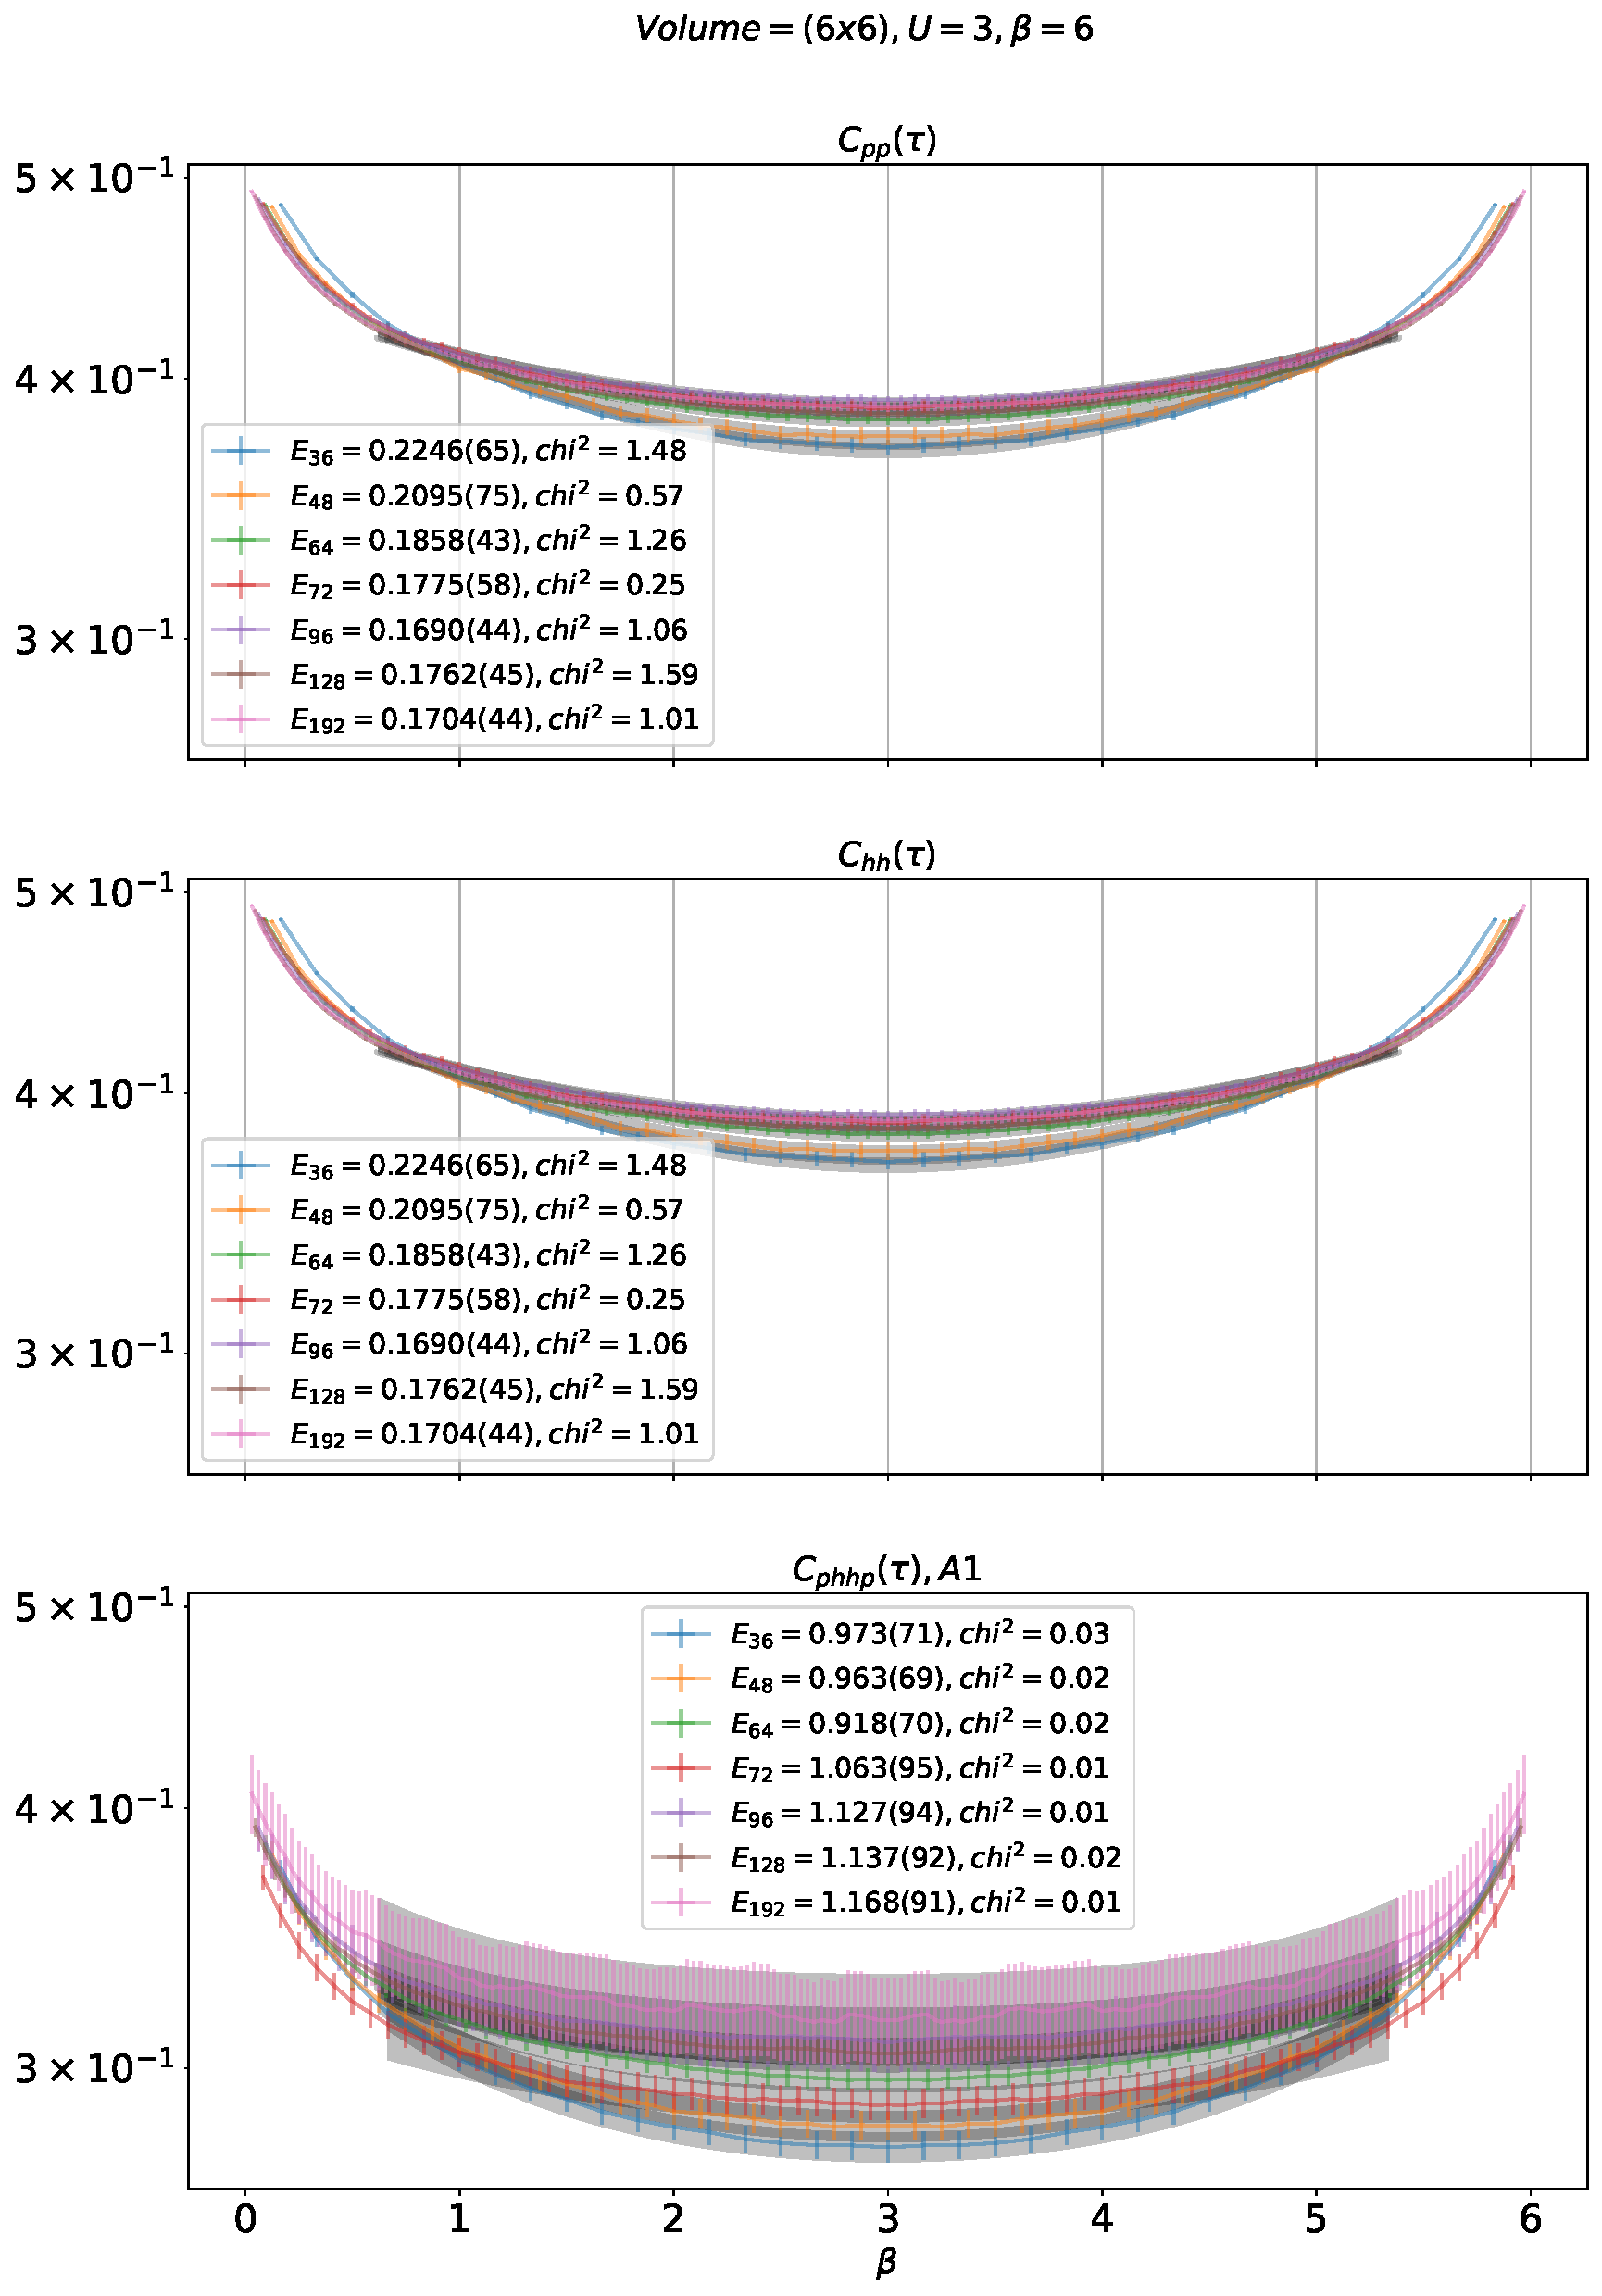
\includegraphics[width=\linewidth]{phhp-0-A1_6x6_U3.0_B6.0.pdf}
  \end{subfigure}%
  \begin{subfigure}{.5\textwidth}
    \centering
    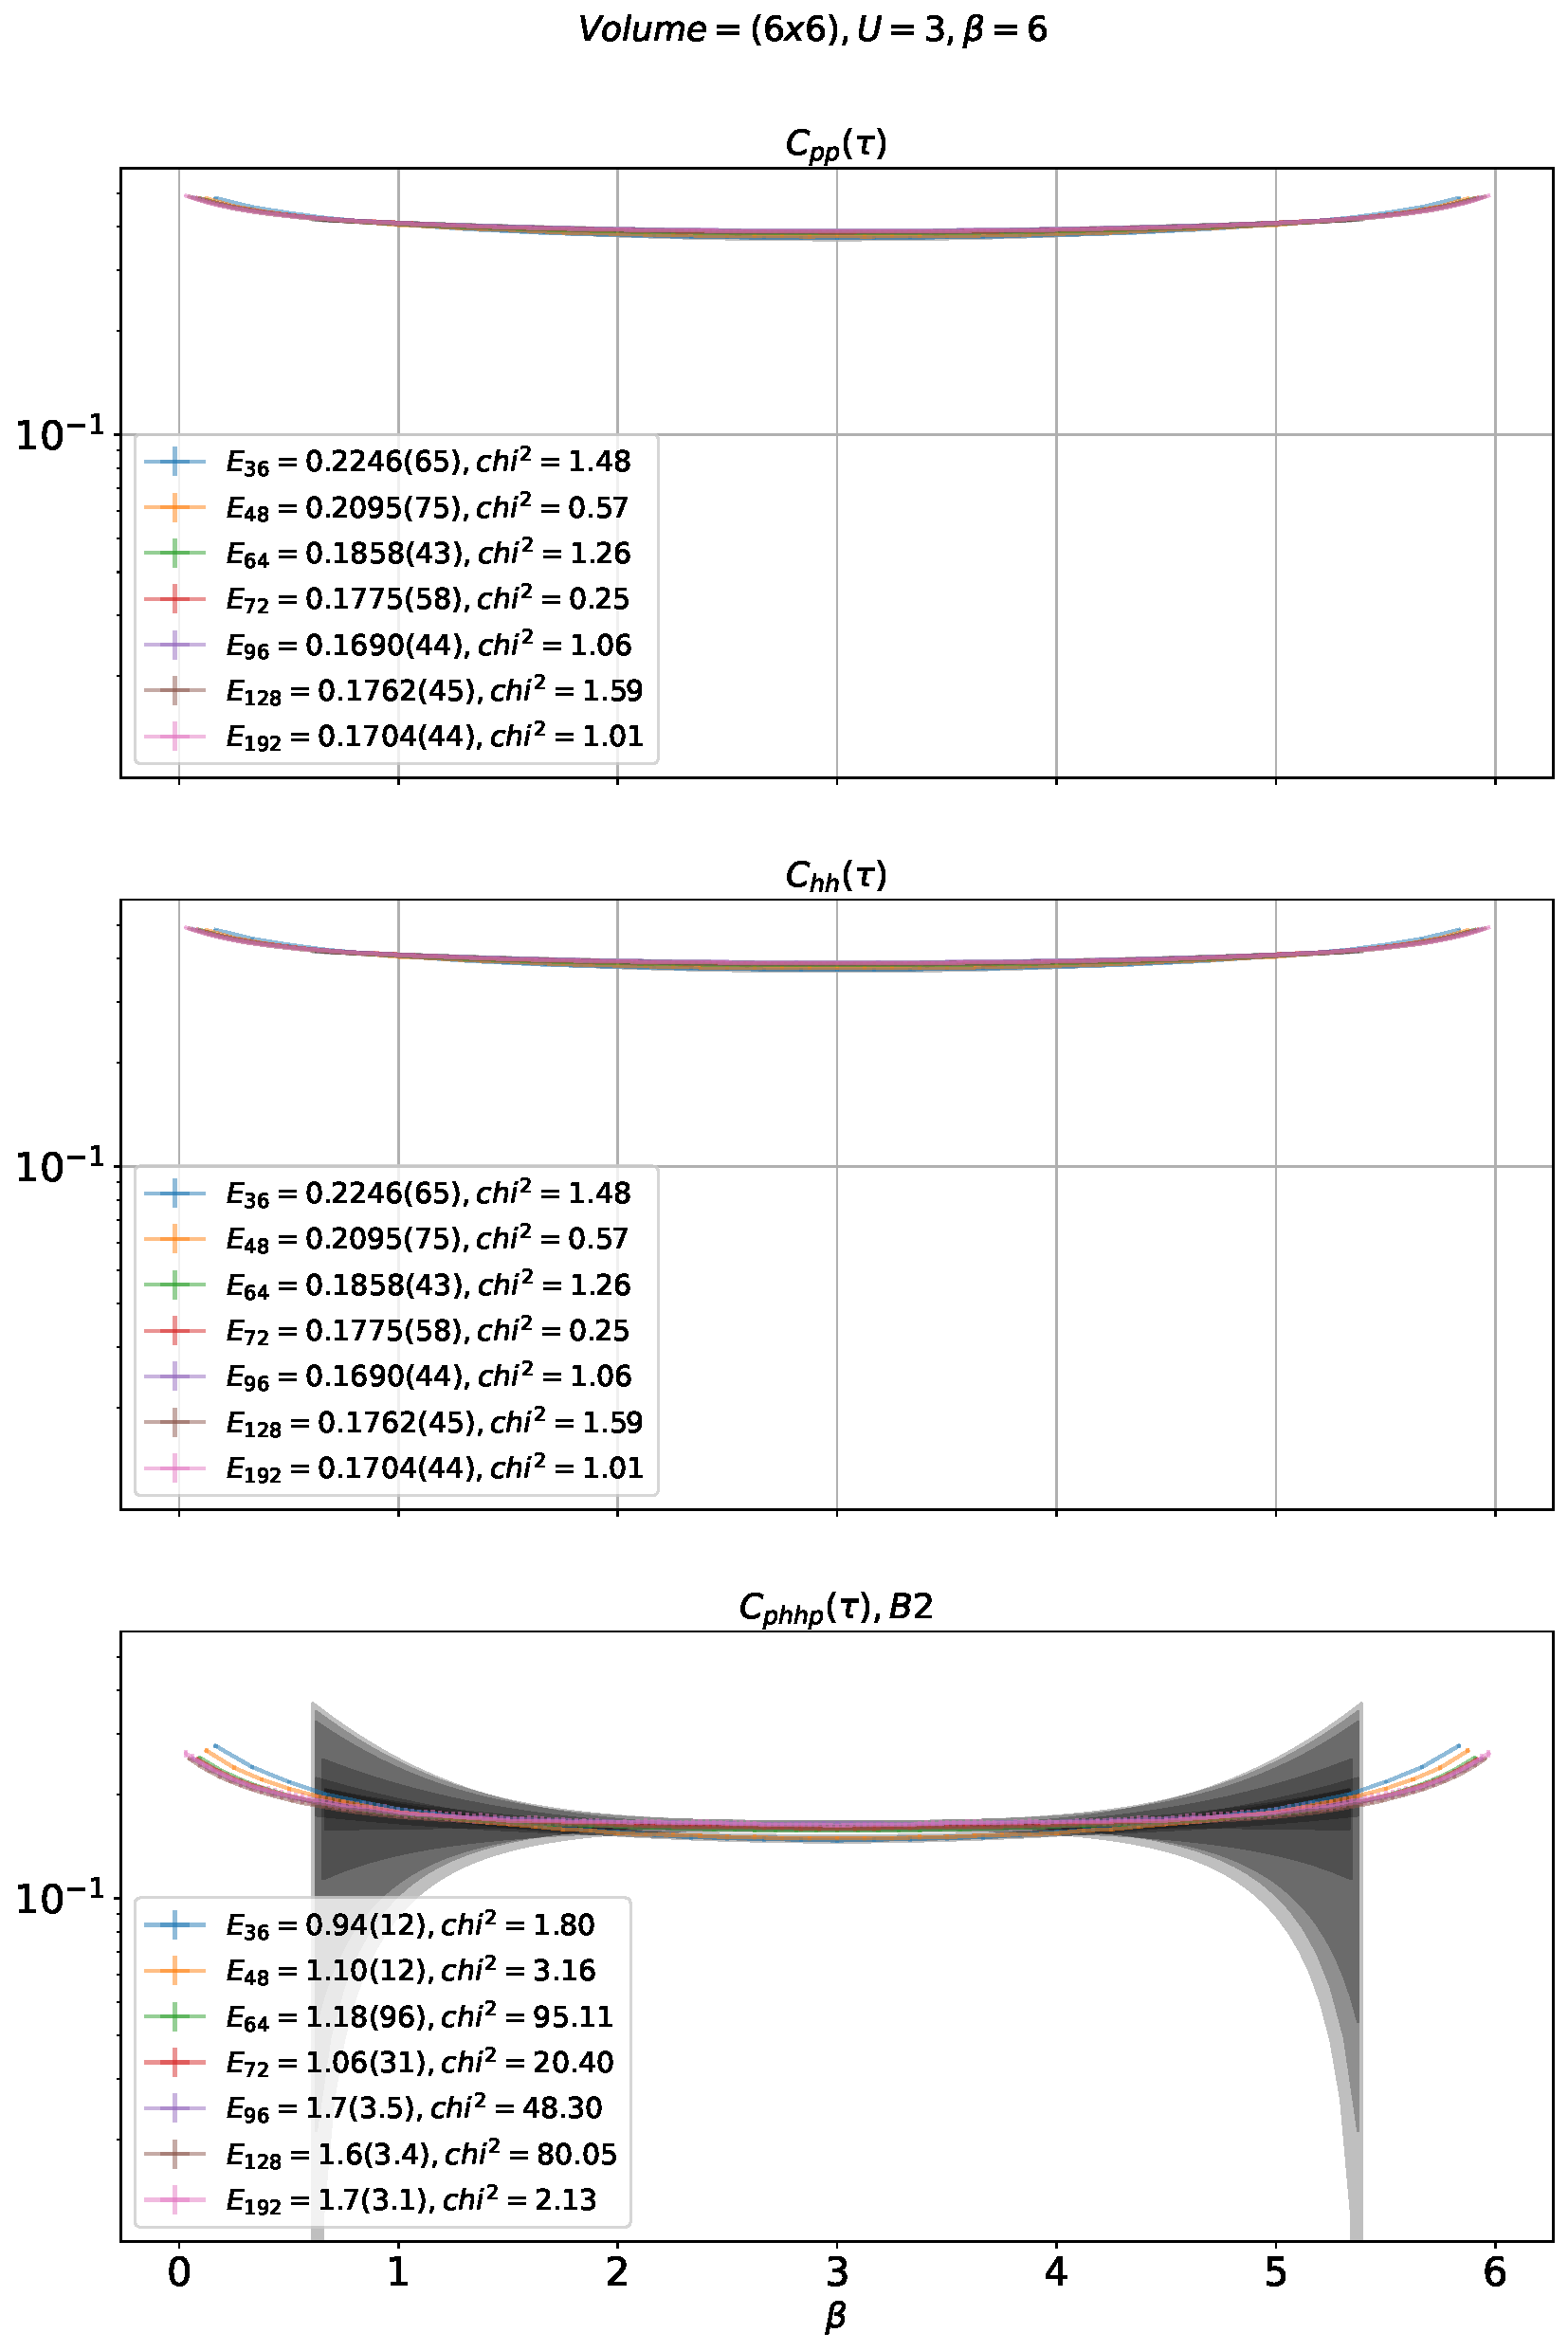
\includegraphics[width=\linewidth]{phhp-0-B2_6x6_U3.0_B6.0.pdf}
  \end{subfigure}
  \begin{subfigure}{.5\textwidth}
      \centering
      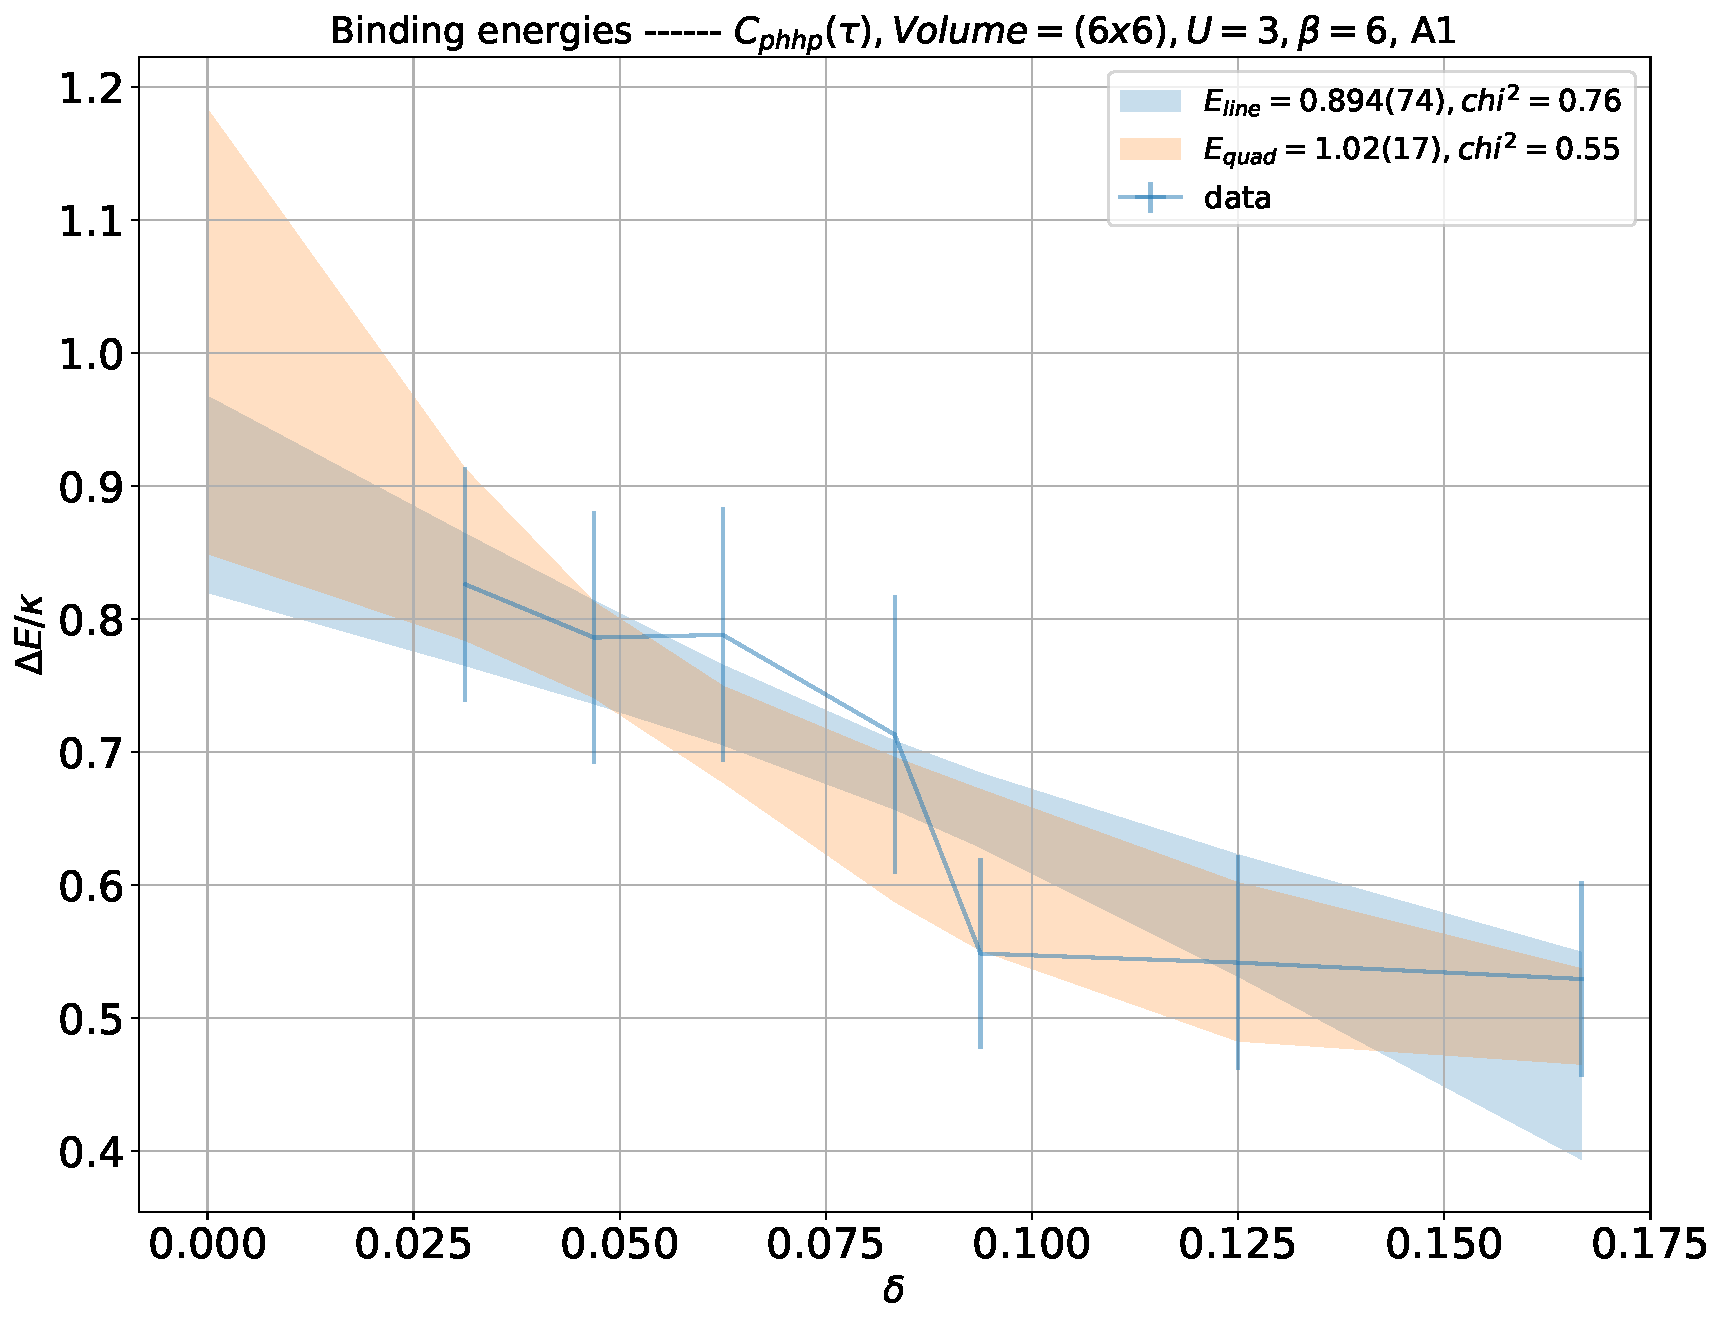
\includegraphics[width=\linewidth]{phhp-0-A1_6x6_U3.0_B6.0_cont.pdf}
  \end{subfigure}
  \begin{subfigure}{.5\textwidth}
      \centering
      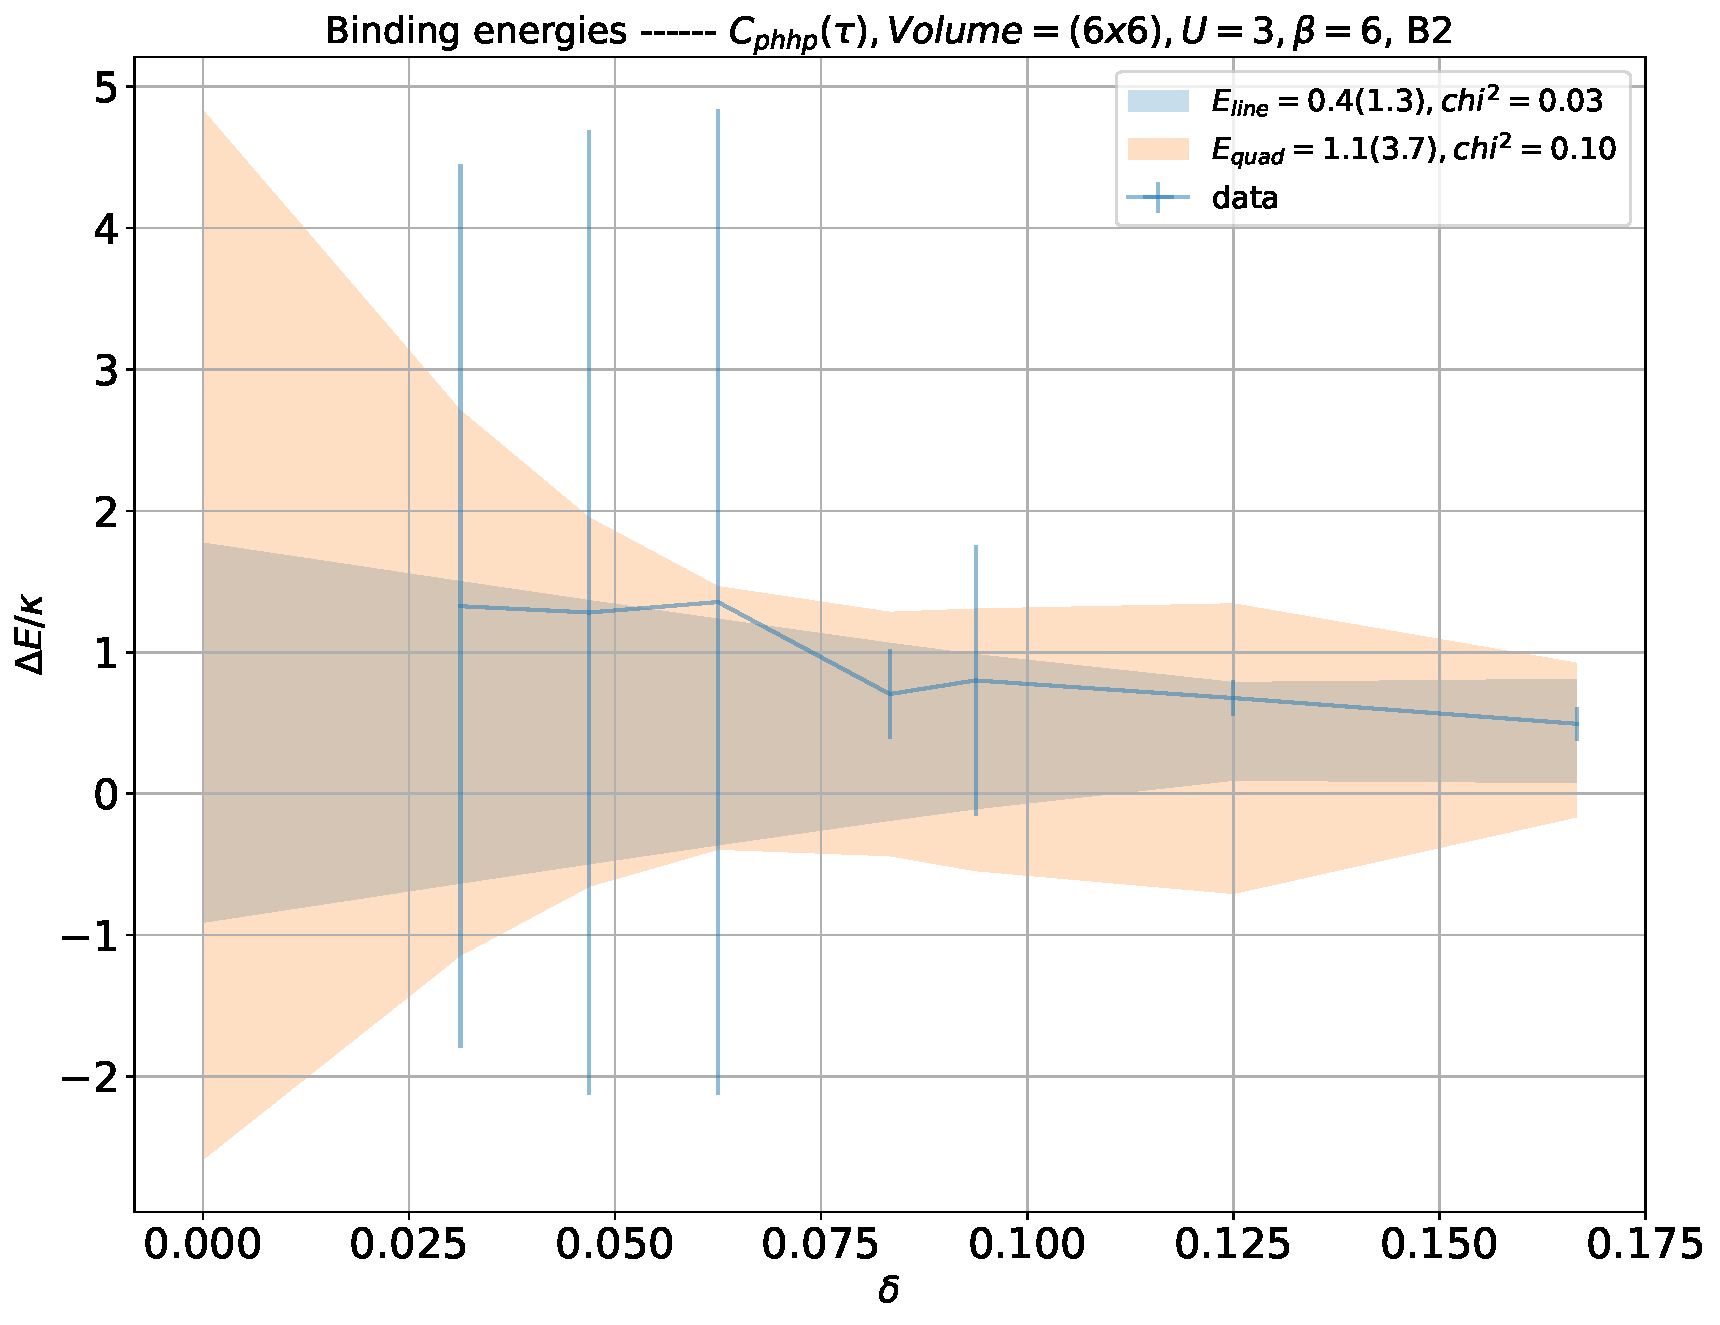
\includegraphics[width=\linewidth]{phhp-0-B2_6x6_U3.0_B6.0_cont.pdf}
  \end{subfigure}
  \caption{Binding energy extraction of the particle-hole pair at both irreducible representations, where we fit one- and two-body correlators for every $N_t$. This is followed by fitting a linear and a quadratic functions to the $\Delta E_{N_t}$ in order to extrapolate to the continuum limit ($N_t\to\infty$).}
  \label{fig:fig1}
\end{figure}

\begin{figure}
  \begin{subfigure}{.5\textwidth}
    \centering
    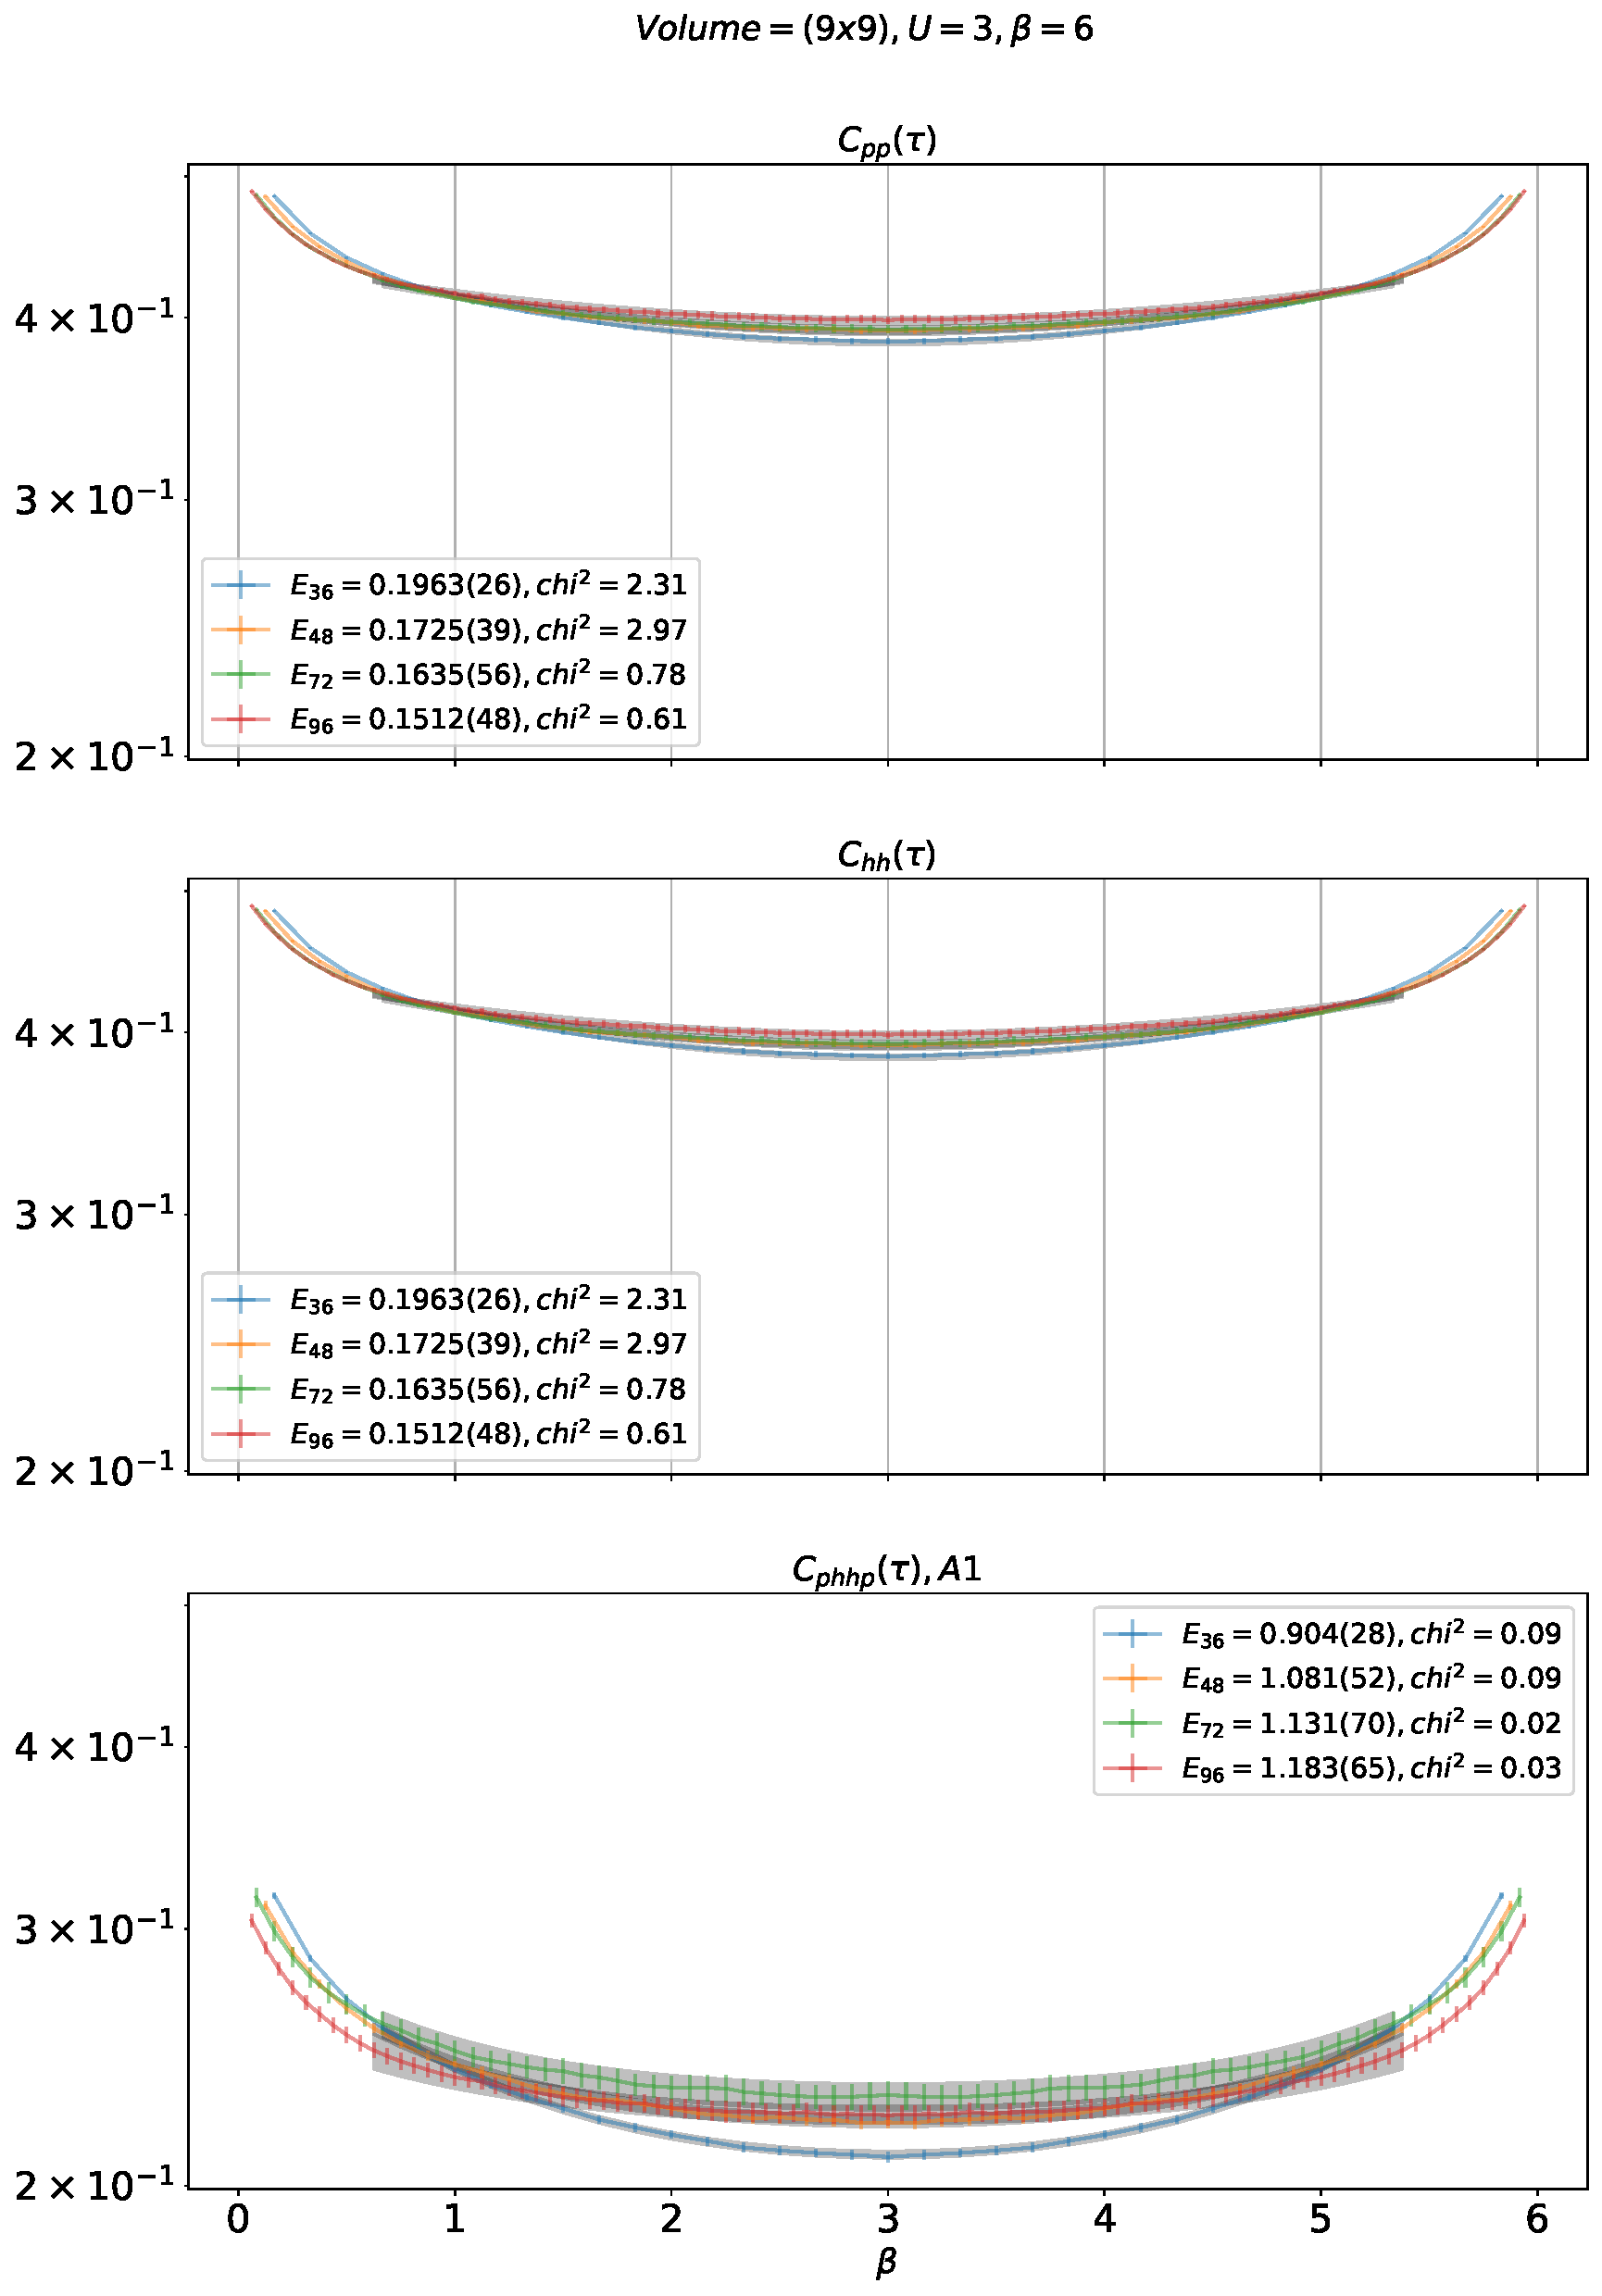
\includegraphics[width=\linewidth]{phhp-0-A1_9x9_U3_B6.pdf}
  \end{subfigure}%
  \begin{subfigure}{.5\textwidth}
    \centering
    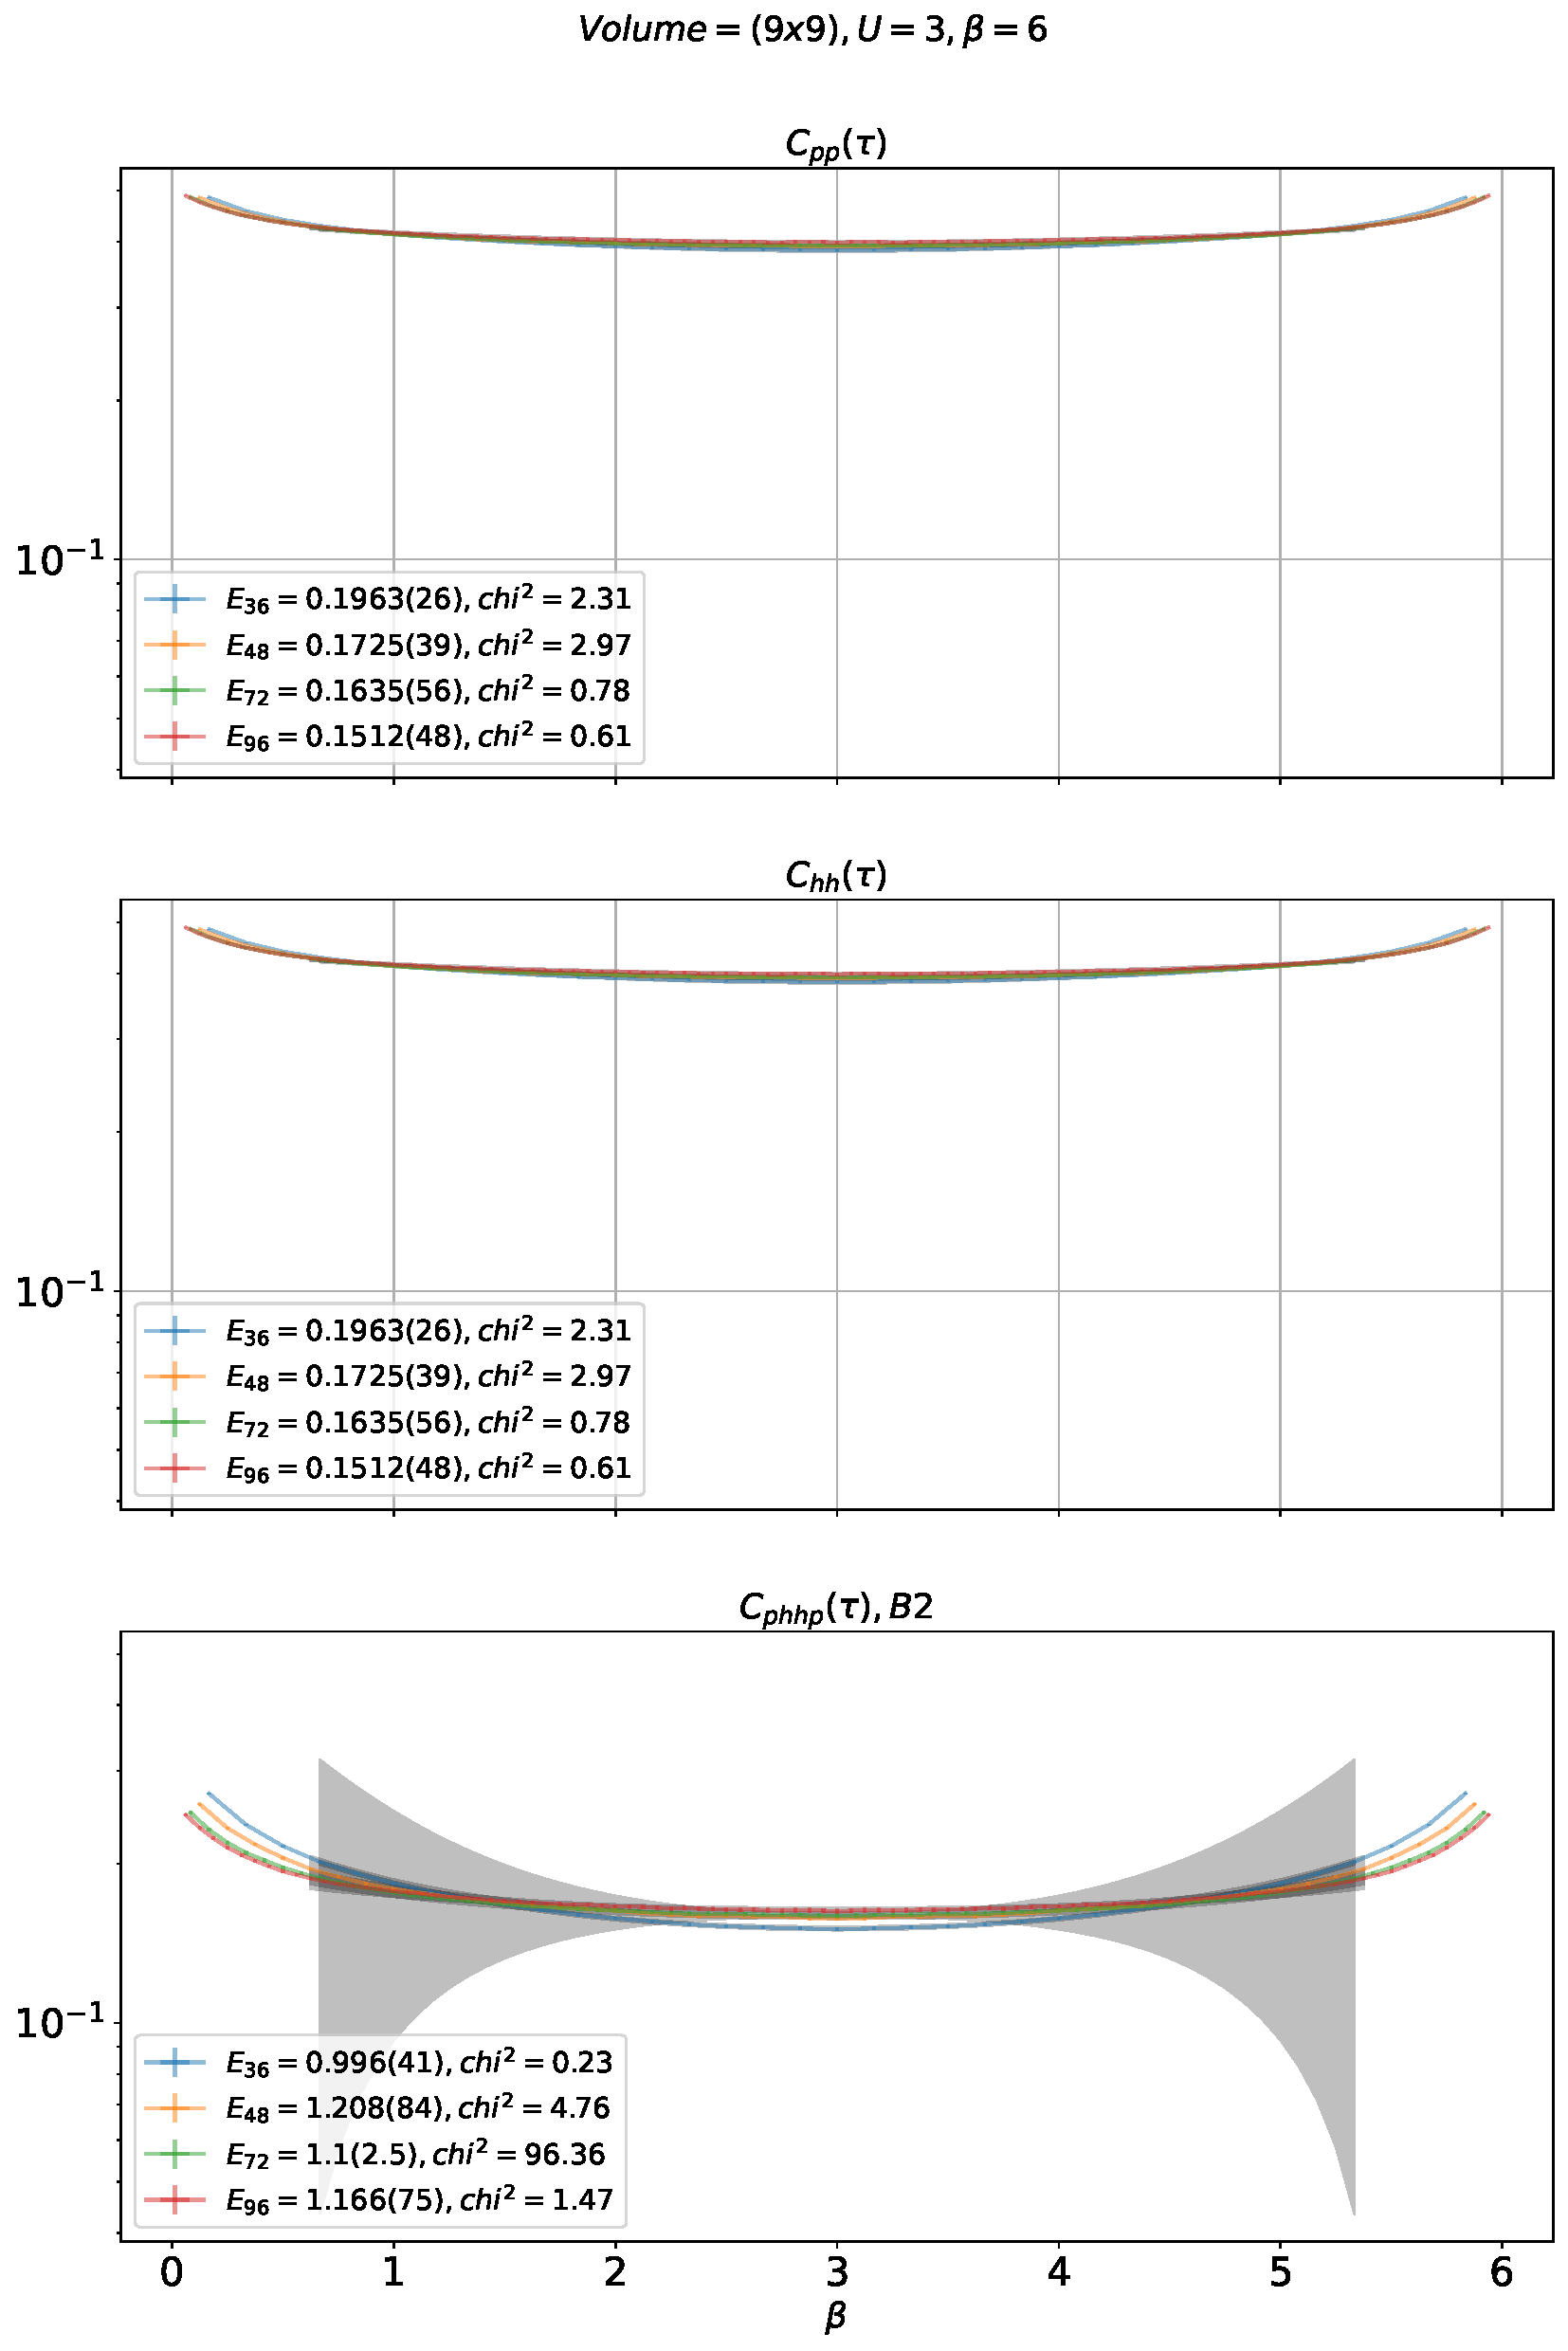
\includegraphics[width=\linewidth]{phhp-0-B2_9x9_U3_B6.pdf}
  \end{subfigure}
  \begin{subfigure}{.5\textwidth}
      \centering
      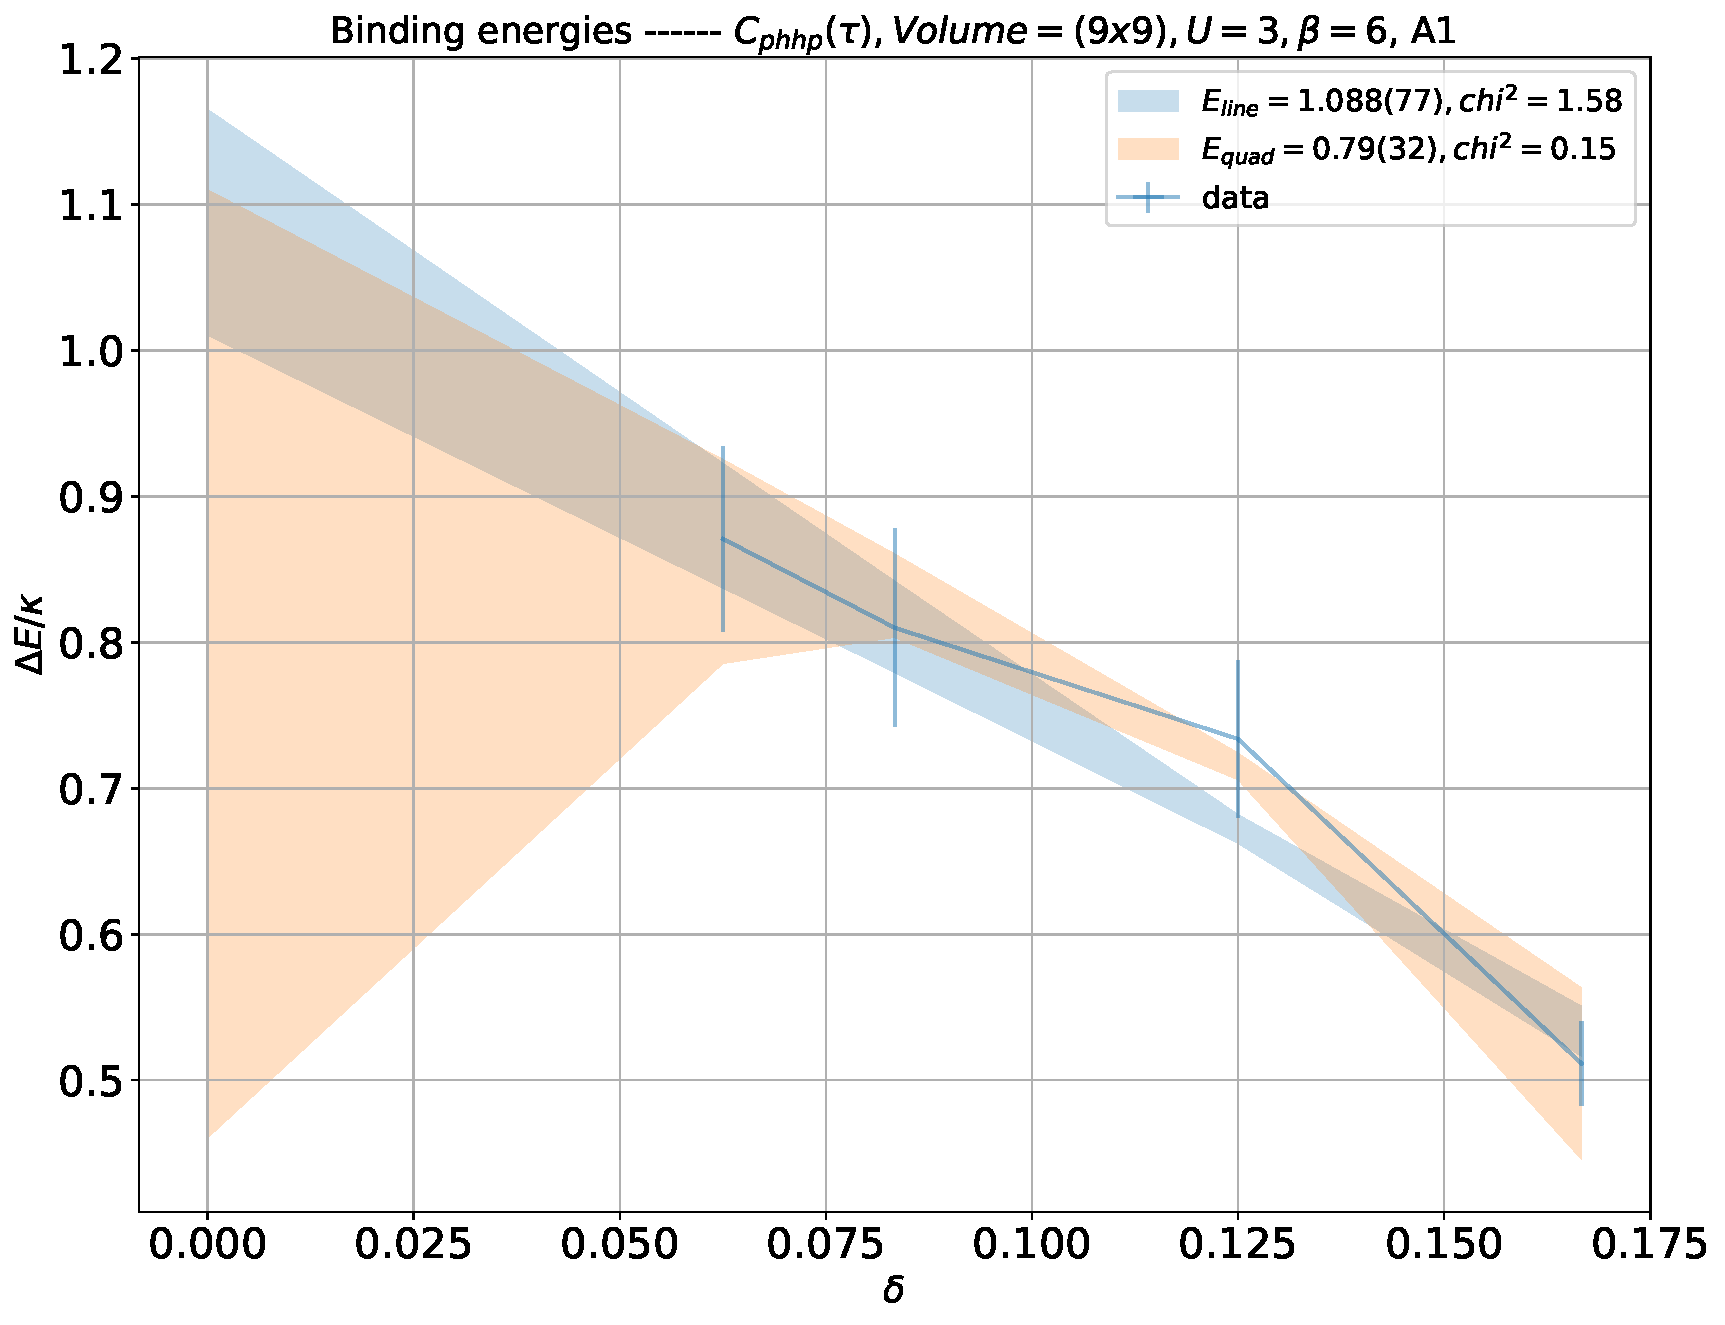
\includegraphics[width=\linewidth]{phhp-0-A1_9x9_U3_B6_cont.pdf}
  \end{subfigure}
  \begin{subfigure}{.5\textwidth}
      \centering
      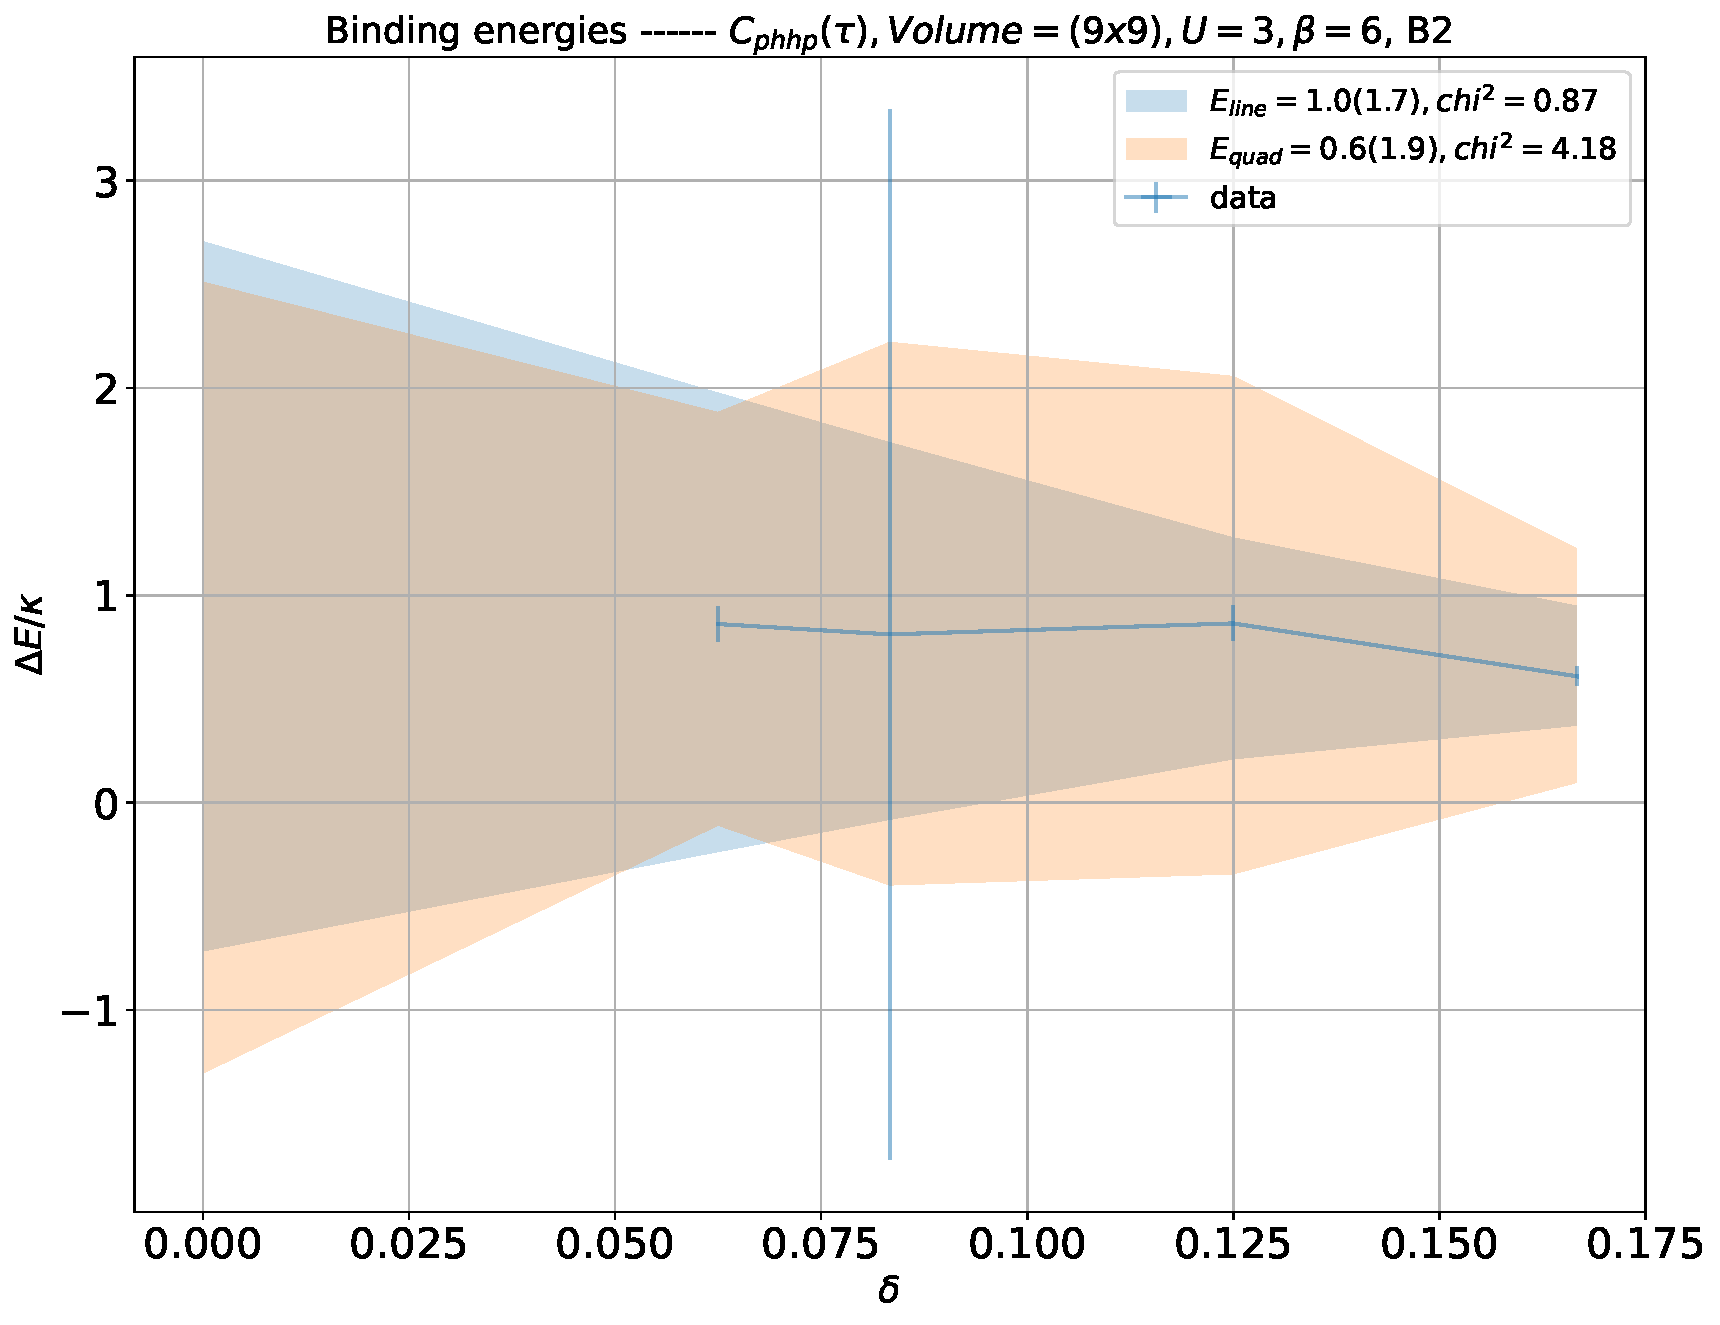
\includegraphics[width=\linewidth]{phhp-0-B2_9x9_U3_B6_cont.pdf}
  \end{subfigure}
  \caption{Binding energy extraction of the particle-hole pair at both irreducible representations, where we fit one- and two-body correlators for every $N_t$. This is followed by fitting a linear and a quadratic functions to the $\Delta E_{N_t}$ in order to extrapolate to the continuum limit ($N_t\to\infty$).}
  \label{fig:fig2}
\end{figure}

\begin{figure}
  \begin{subfigure}{.5\textwidth}
    \centering
    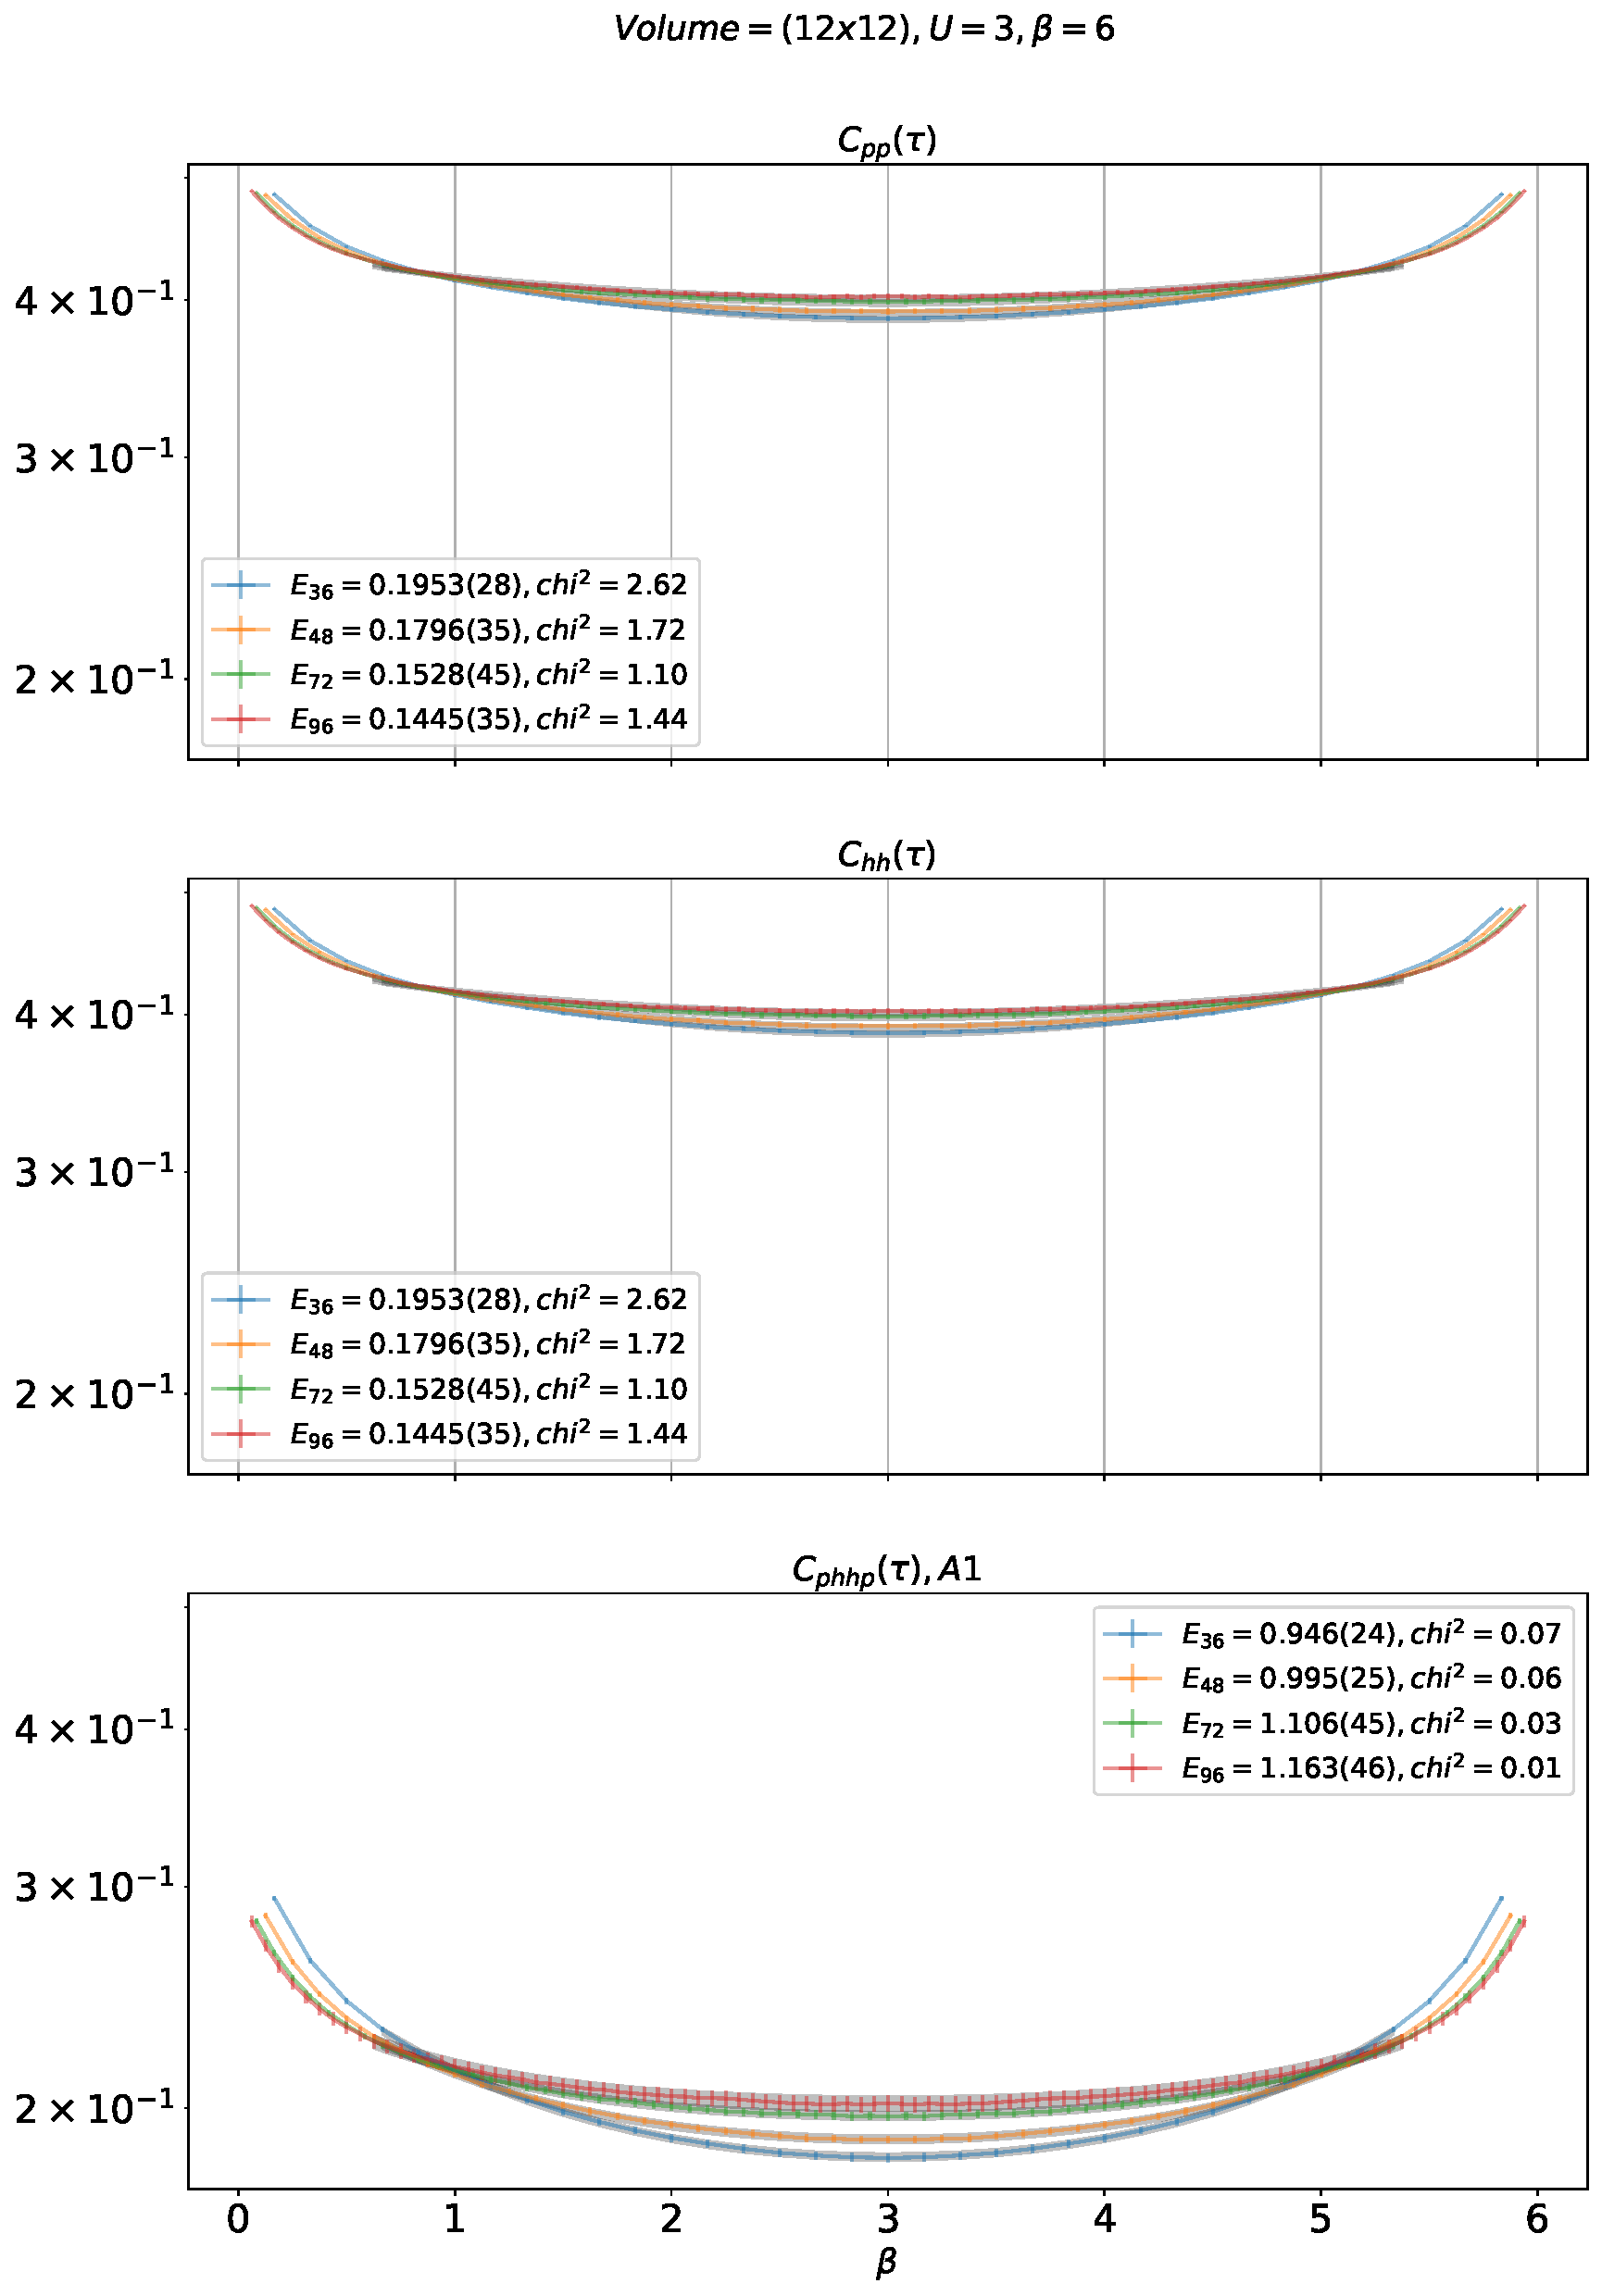
\includegraphics[width=\linewidth]{phhp-0-A1_12x12_U3_B6.pdf}
  \end{subfigure}%
  \begin{subfigure}{.5\textwidth}
    \centering
    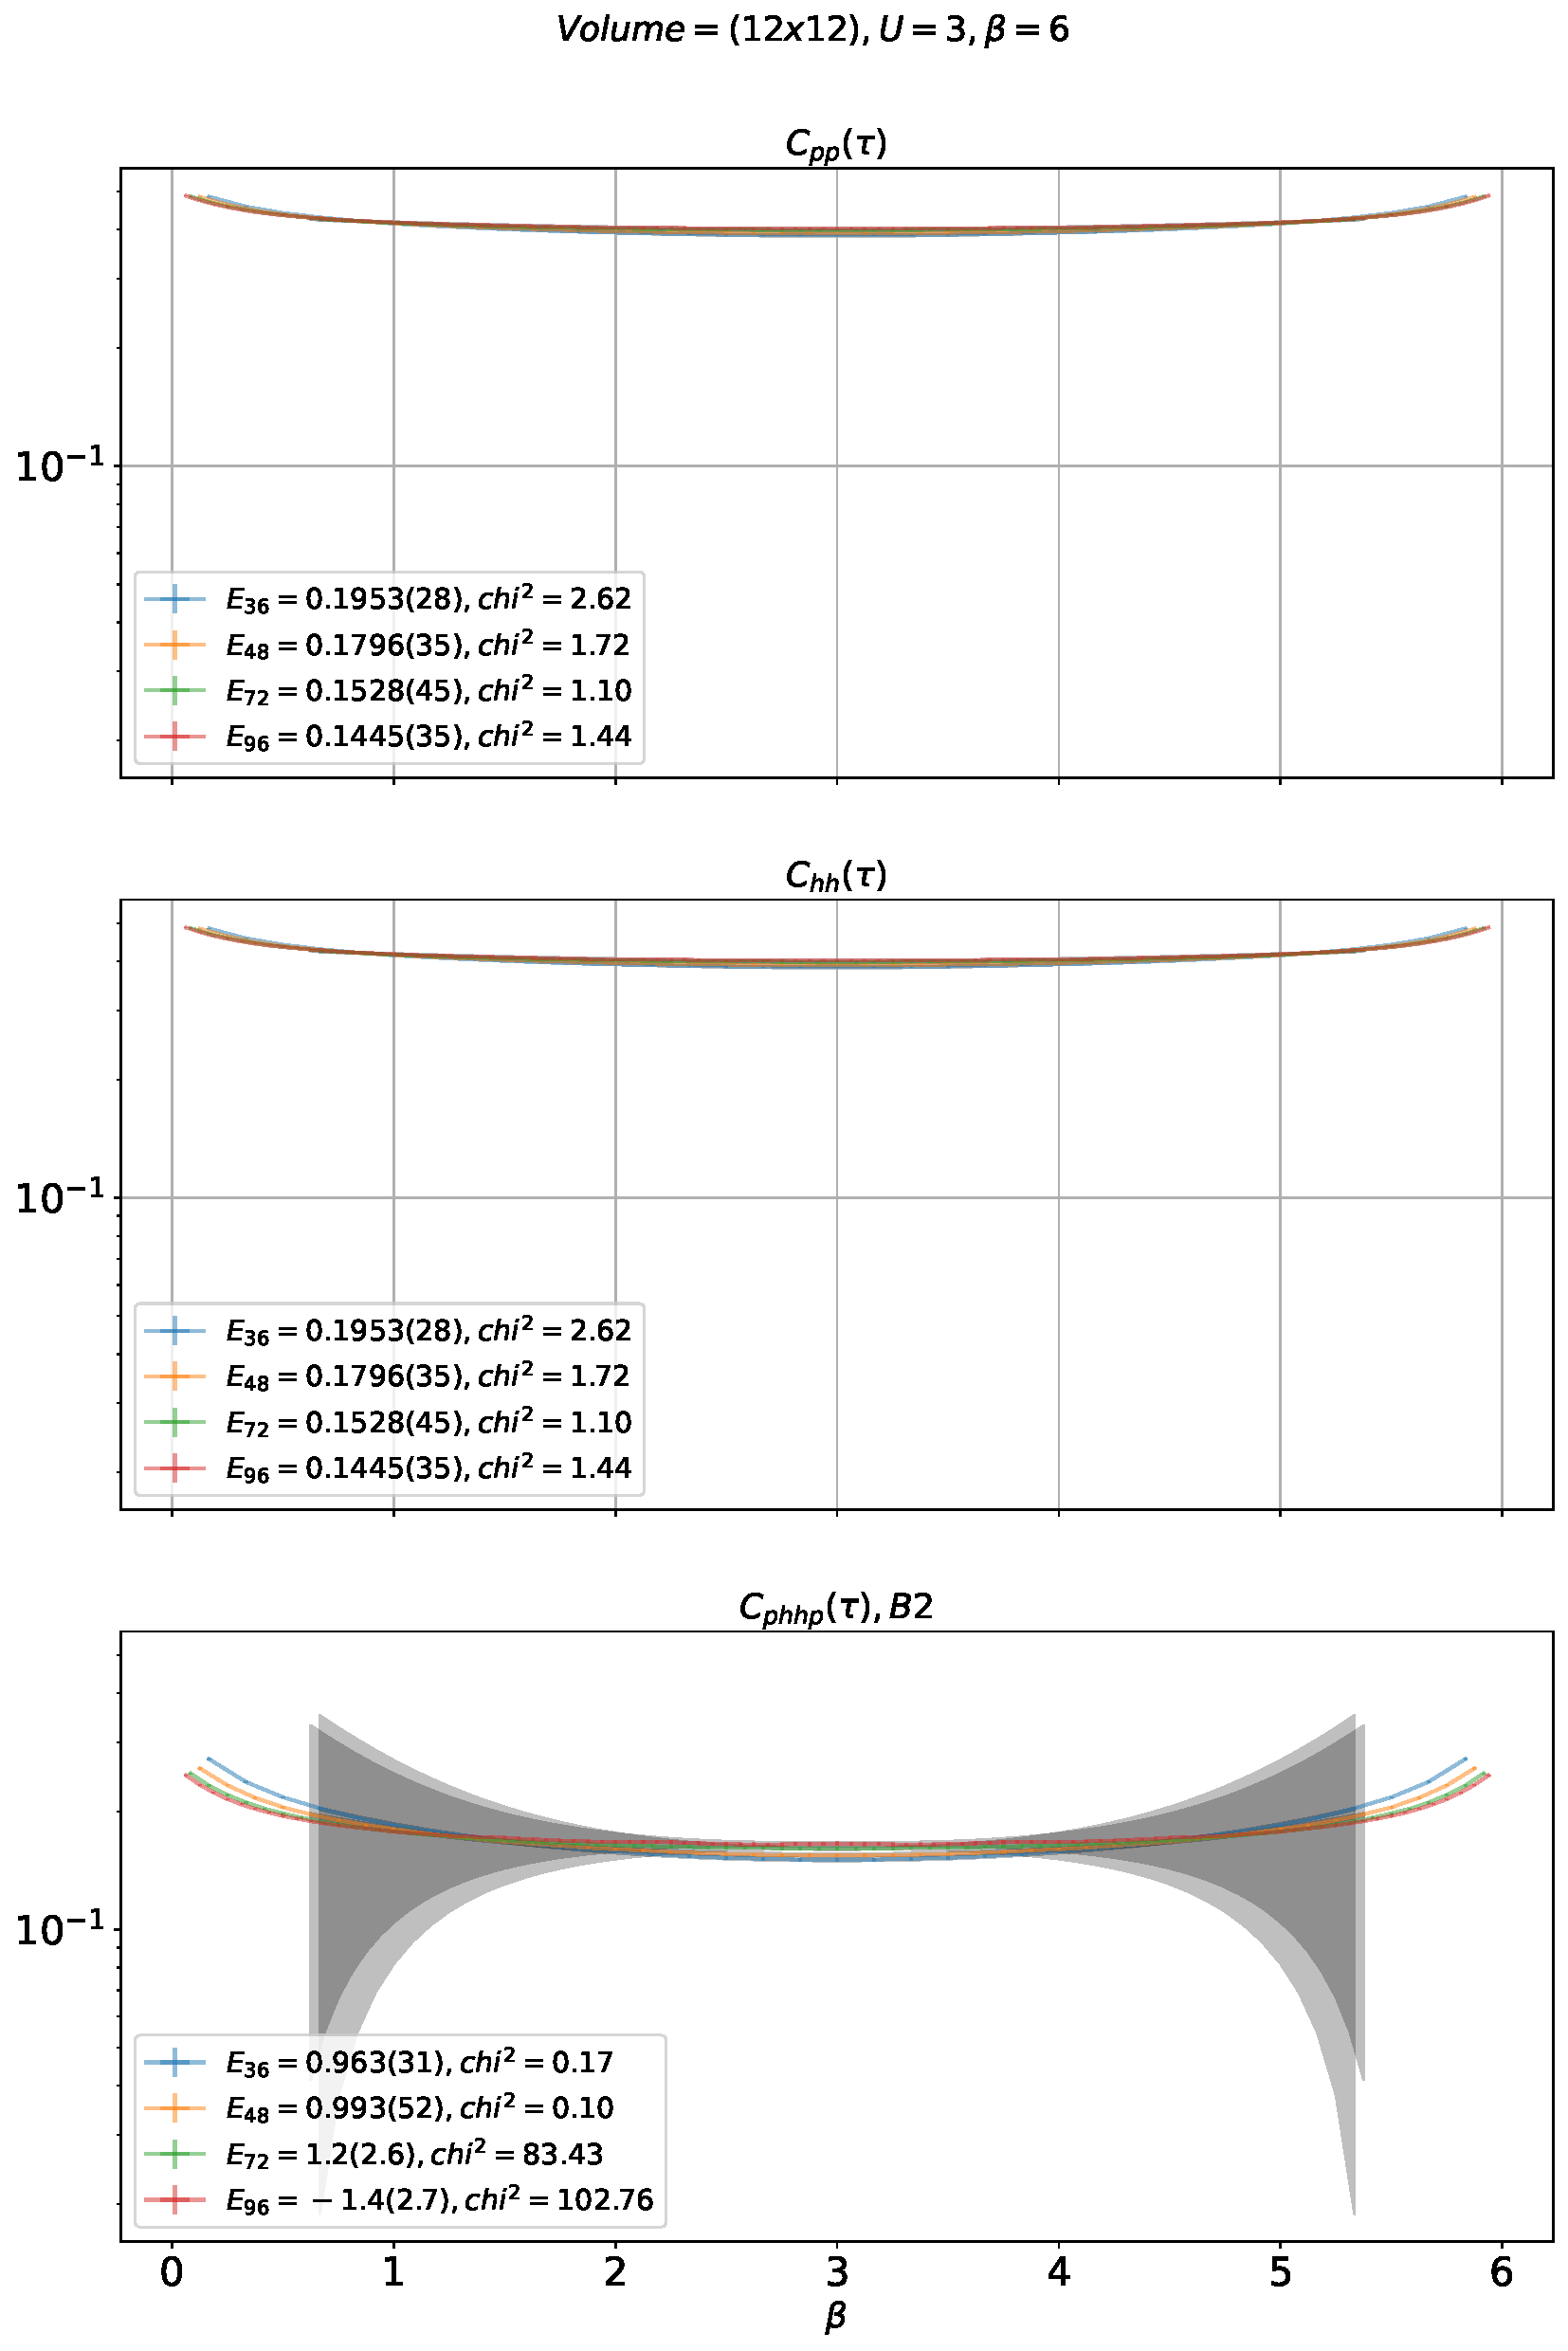
\includegraphics[width=\linewidth]{phhp-0-B2_12x12_U3_B6.pdf}
  \end{subfigure}
  \begin{subfigure}{.5\textwidth}
      \centering
      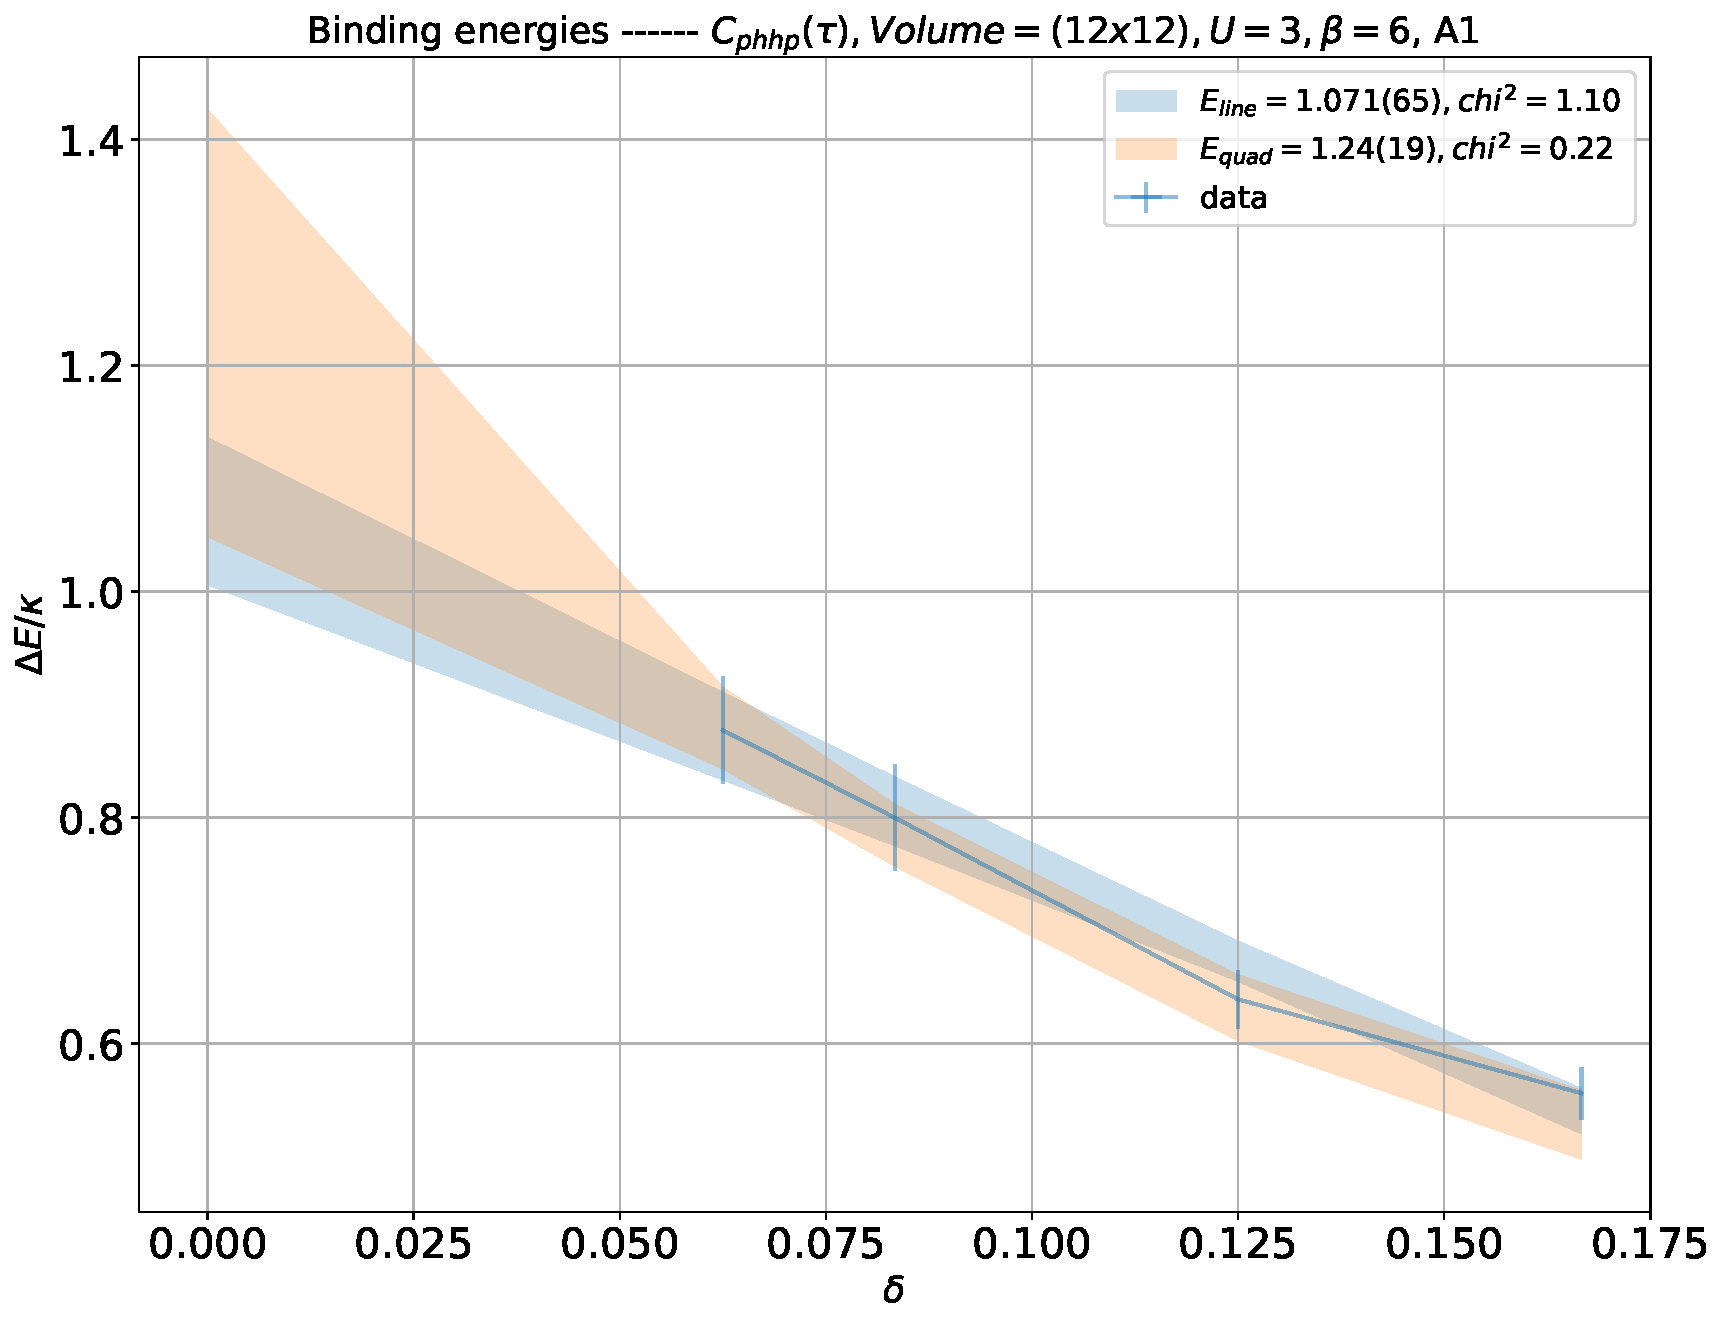
\includegraphics[width=\linewidth]{phhp-0-A1_12x12_U3_B6_cont.pdf}
  \end{subfigure}
  \begin{subfigure}{.5\textwidth}
      \centering
      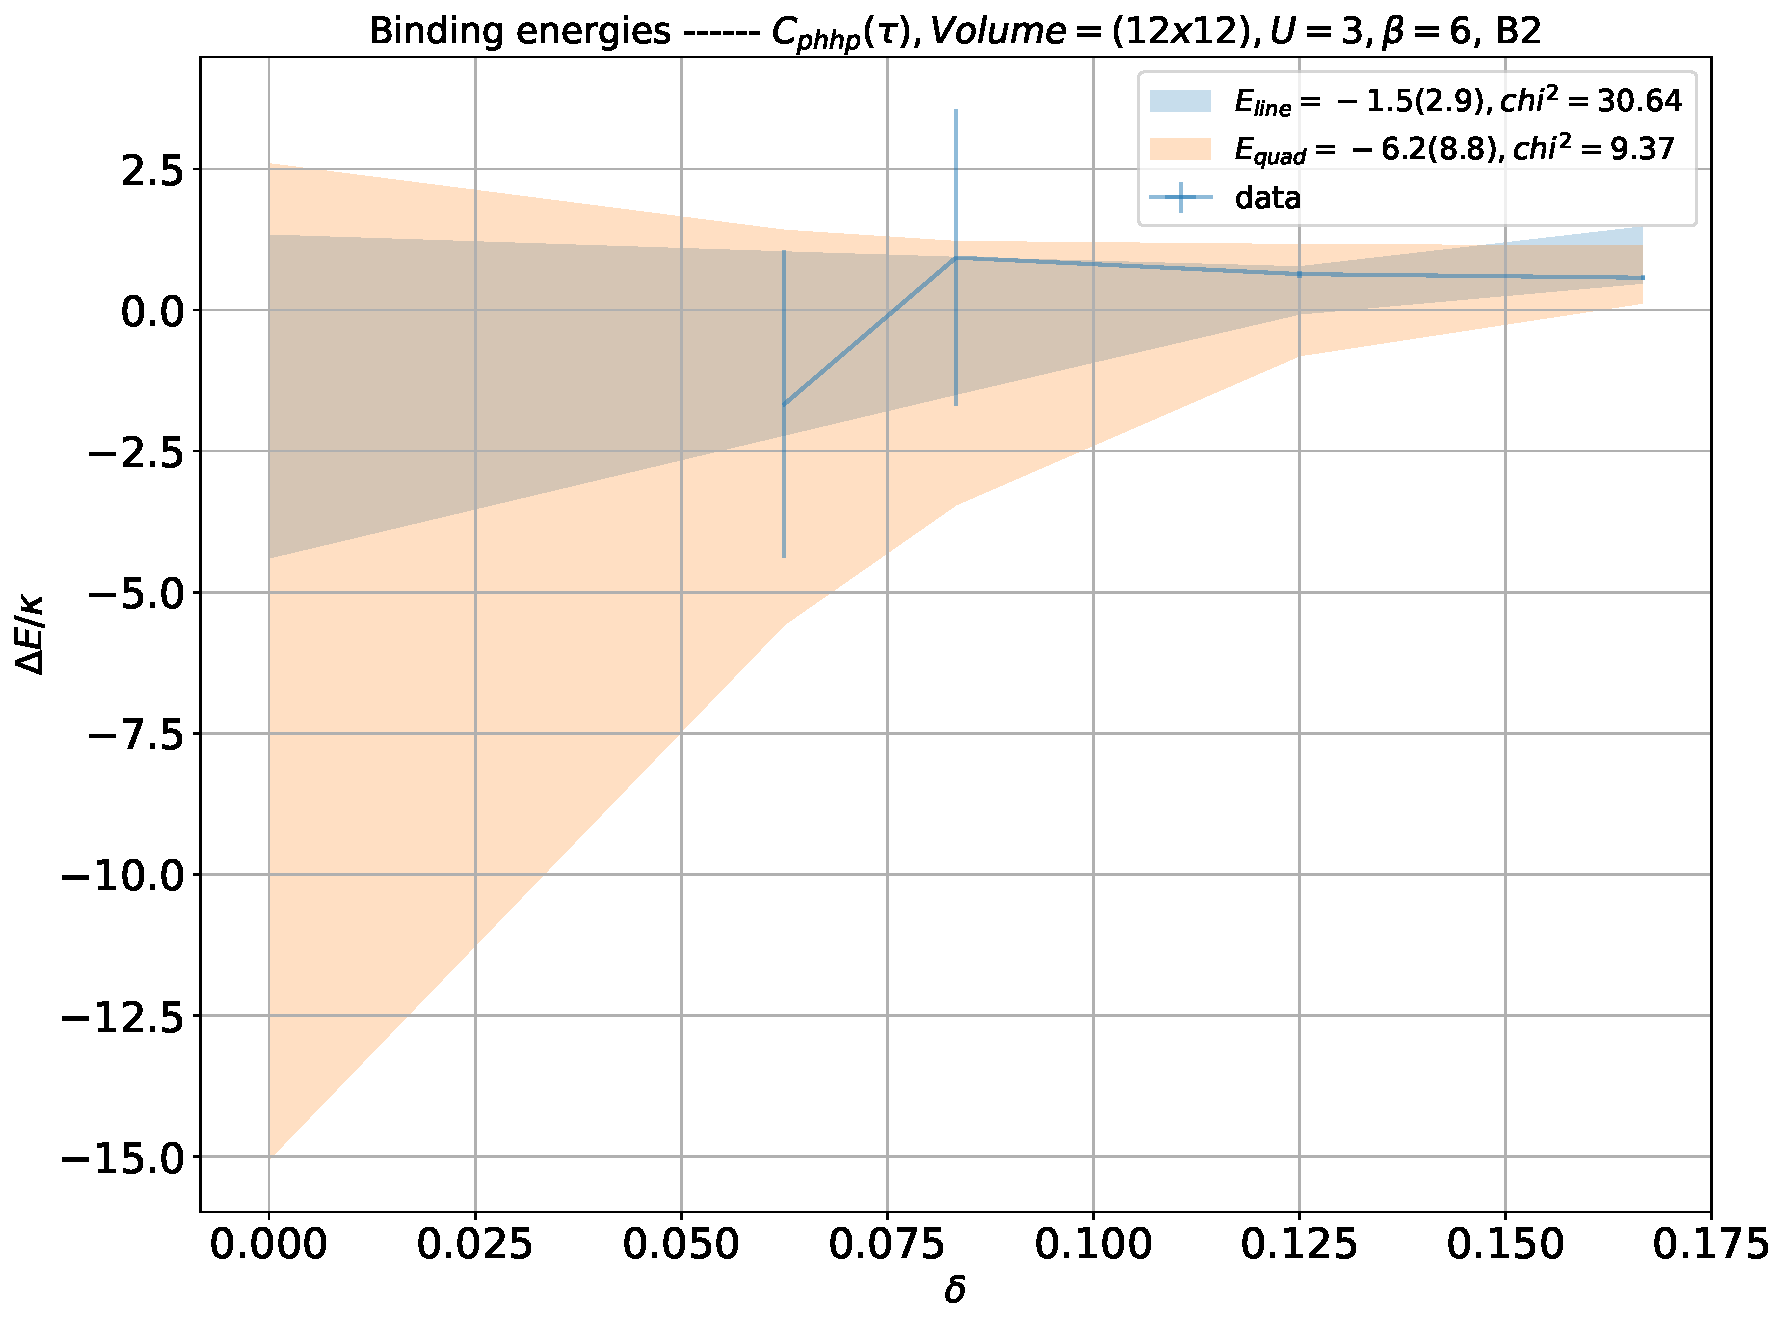
\includegraphics[width=\linewidth]{phhp-0-B2_12x12_U3_B6_cont.pdf}
  \end{subfigure}
  \caption{Binding energy extraction of the particle-hole pair at both irreducible representations, where we fit one- and two-body correlators for every $N_t$. This is followed by fitting a linear and a quadratic functions to the $\Delta E_{N_t}$ in order to extrapolate to the continuum limit ($N_t\to\infty$).}
  \label{fig:fig3}
\end{figure}

\begin{figure}
  \begin{subfigure}{.5\textwidth}
    \centering
    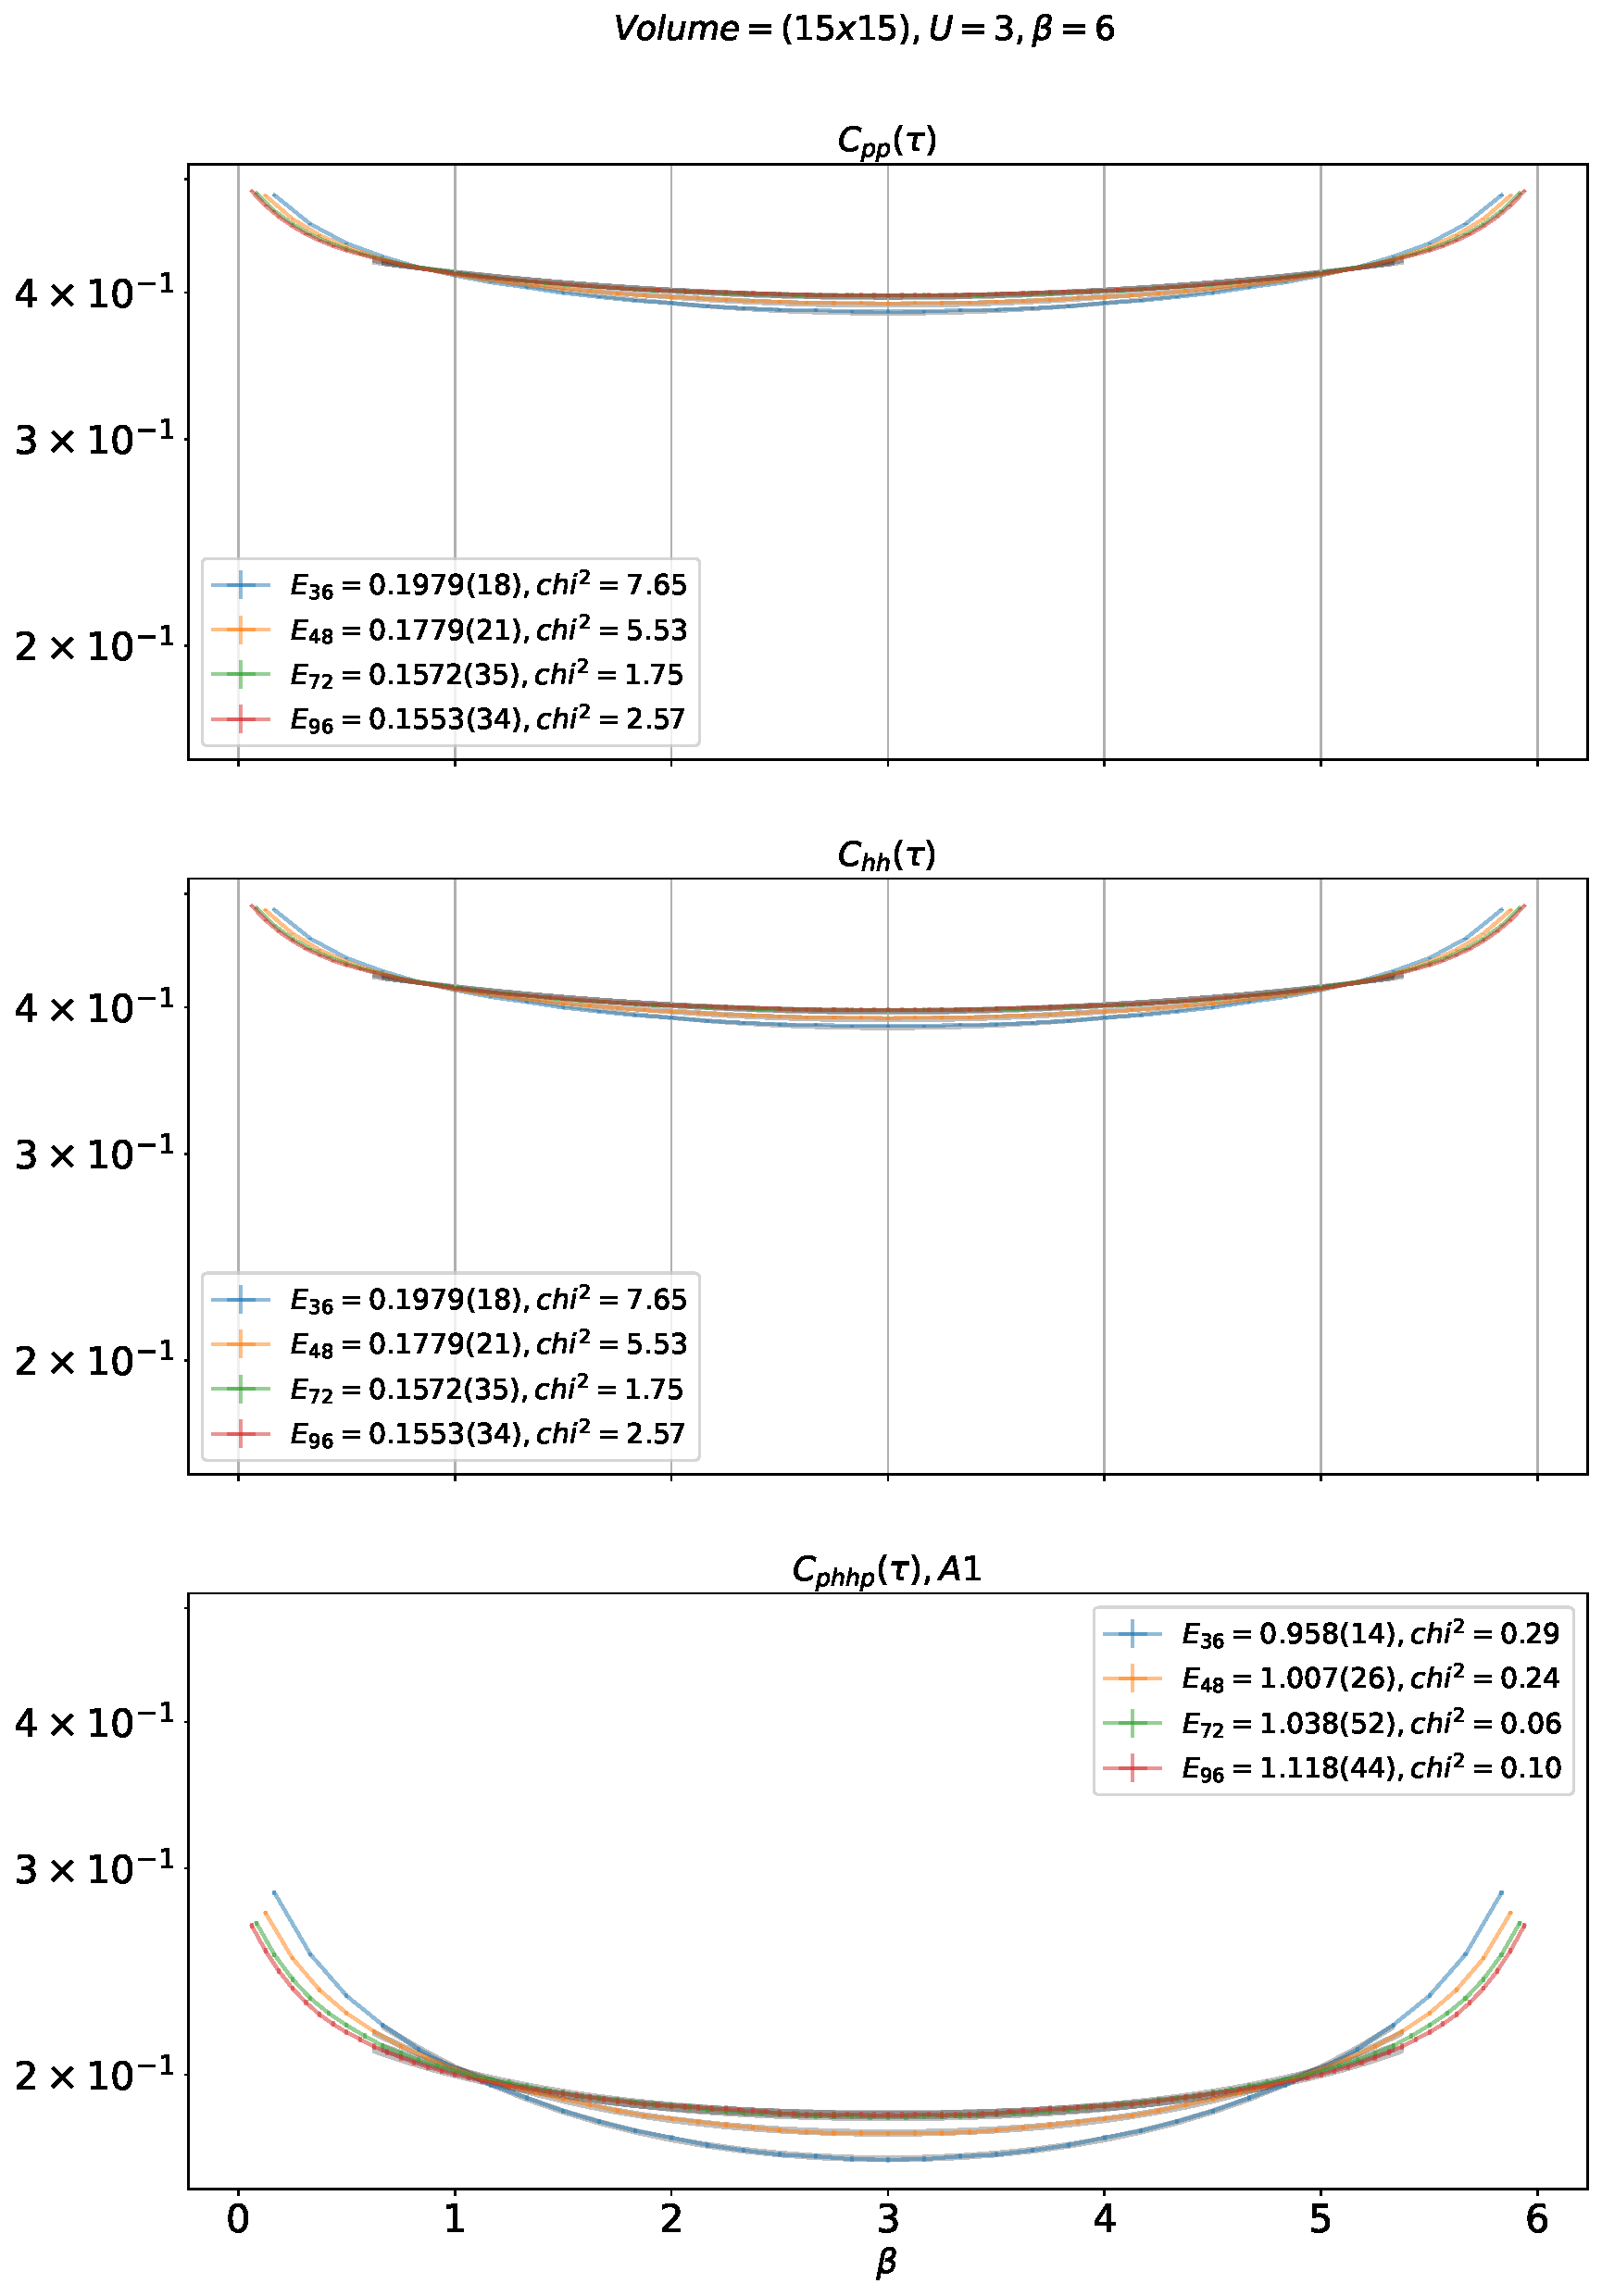
\includegraphics[width=\linewidth]{phhp-0-A1_15x15_U3_B6.pdf}
  \end{subfigure}%
  \begin{subfigure}{.5\textwidth}
    \centering
    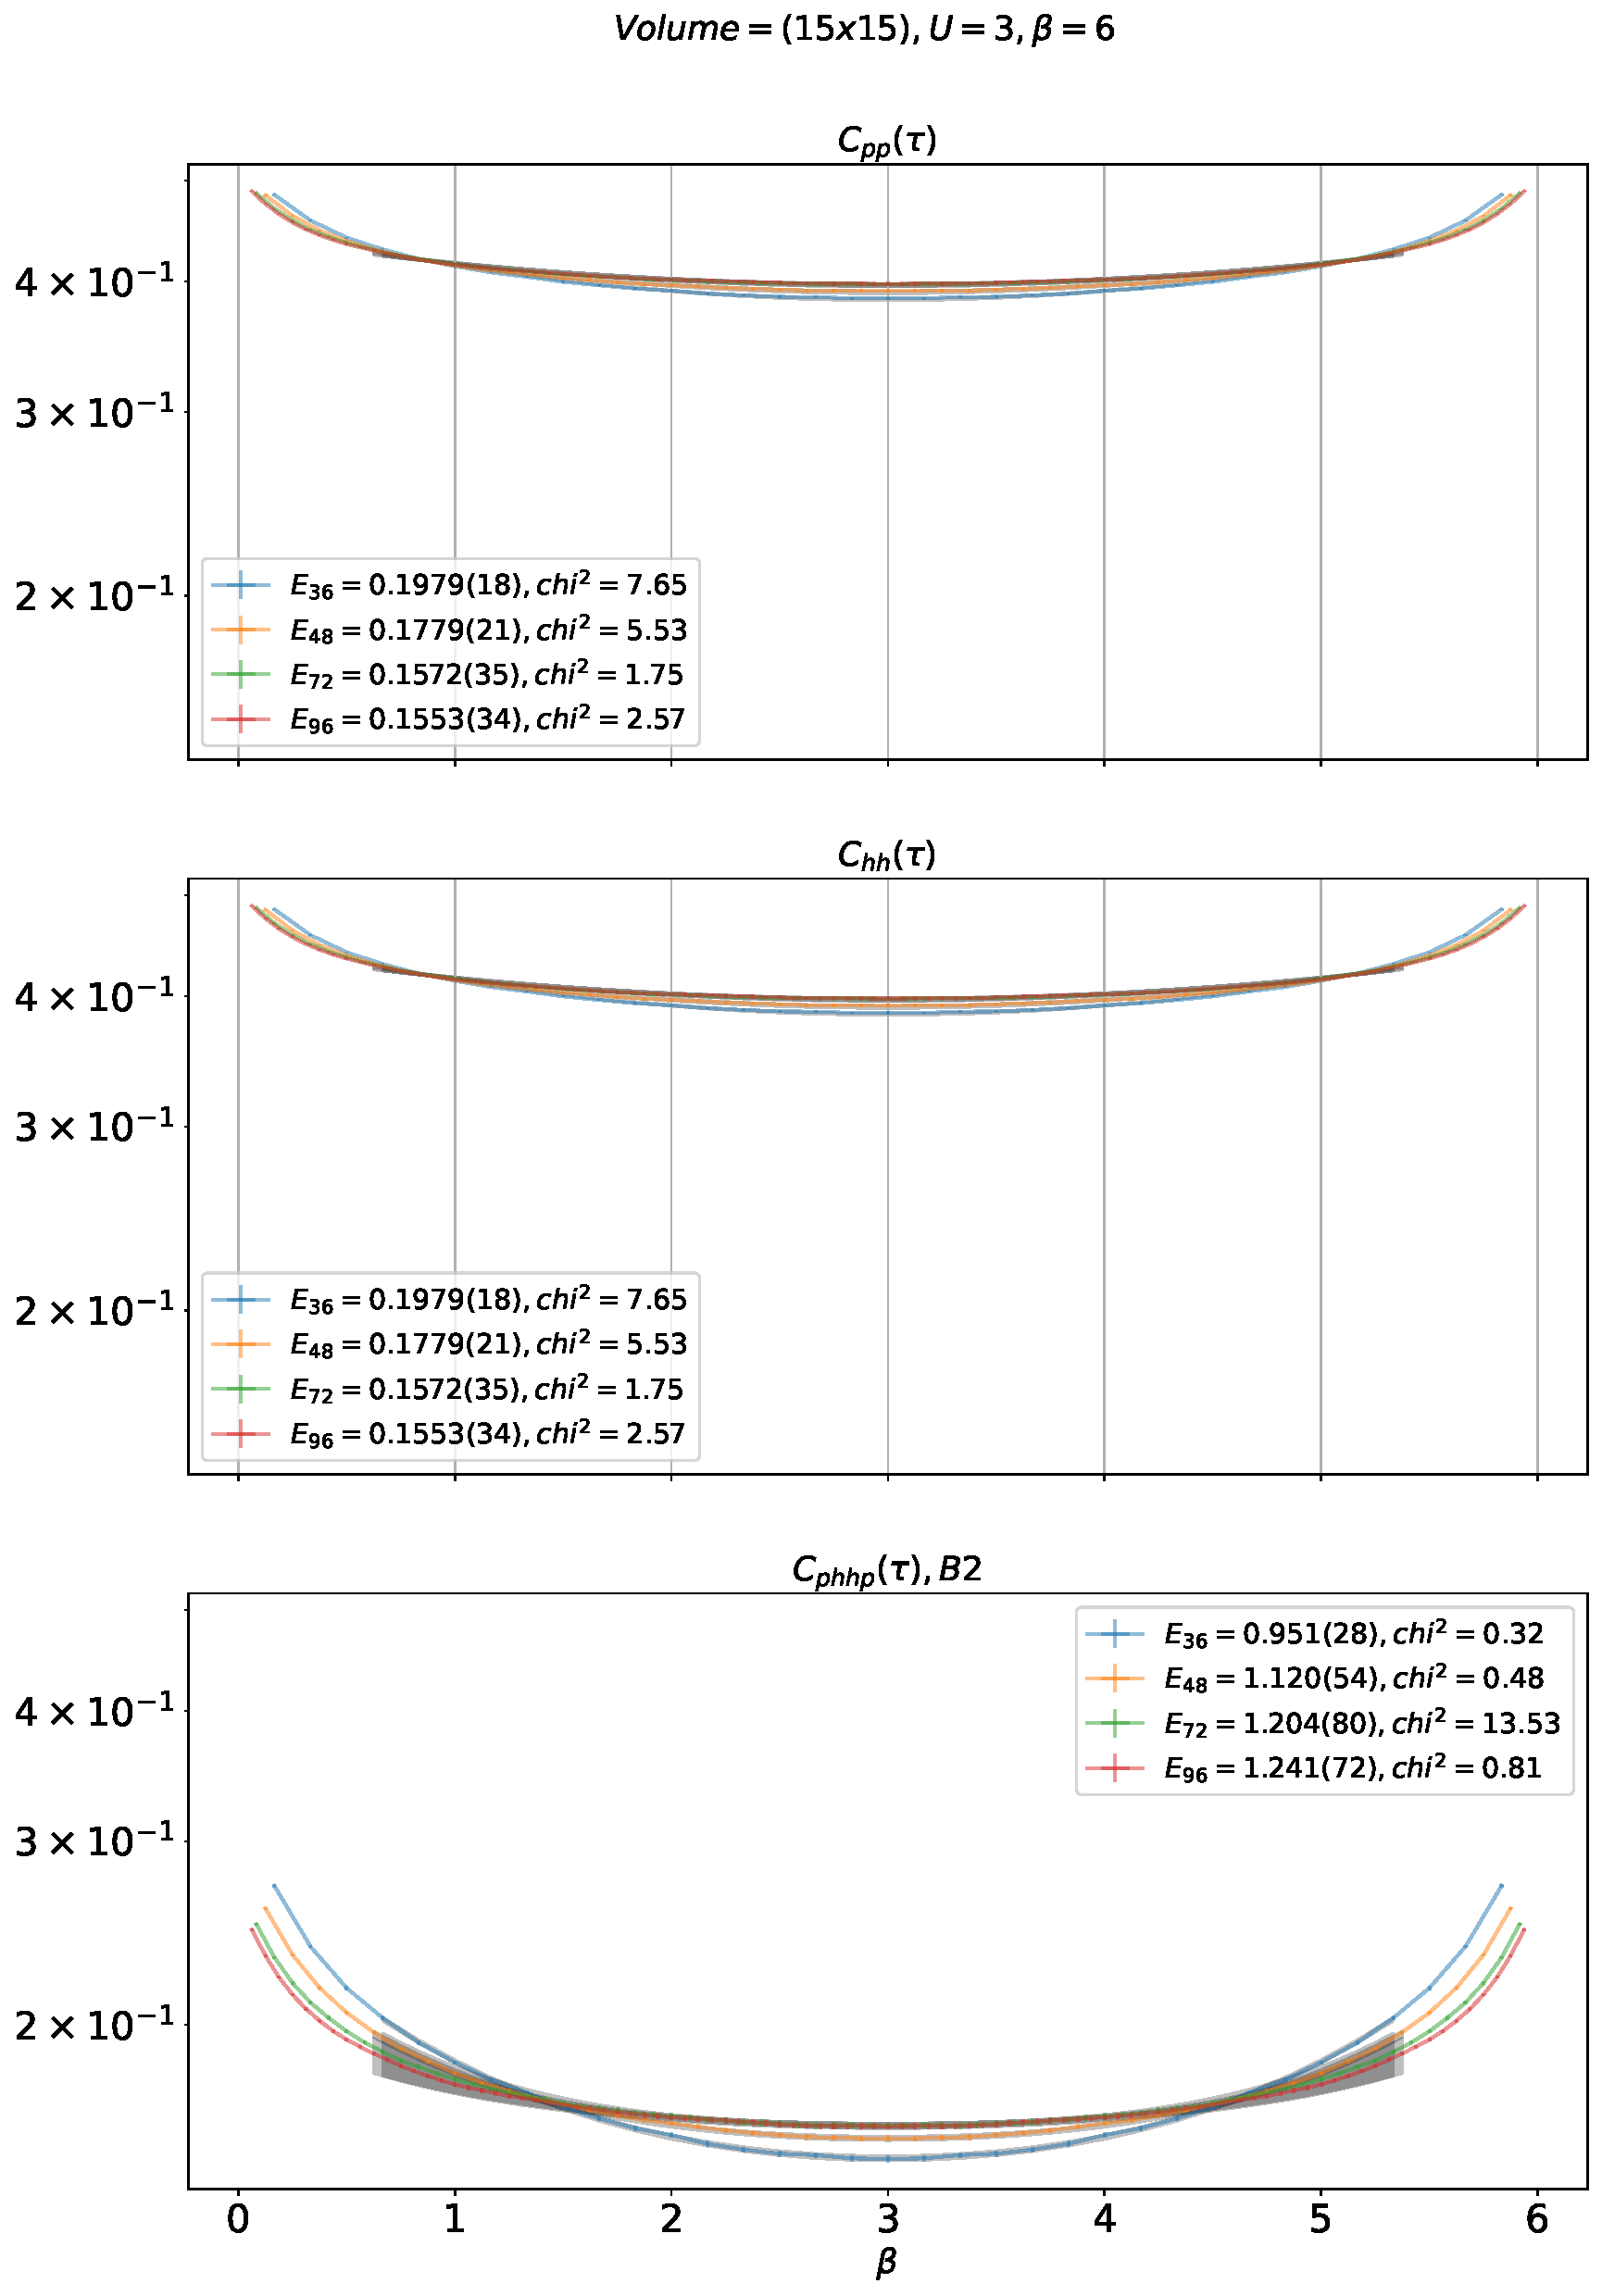
\includegraphics[width=\linewidth]{phhp-0-B2_15x15_U3_B6.pdf}
  \end{subfigure}
  \begin{subfigure}{.5\textwidth}
      \centering
      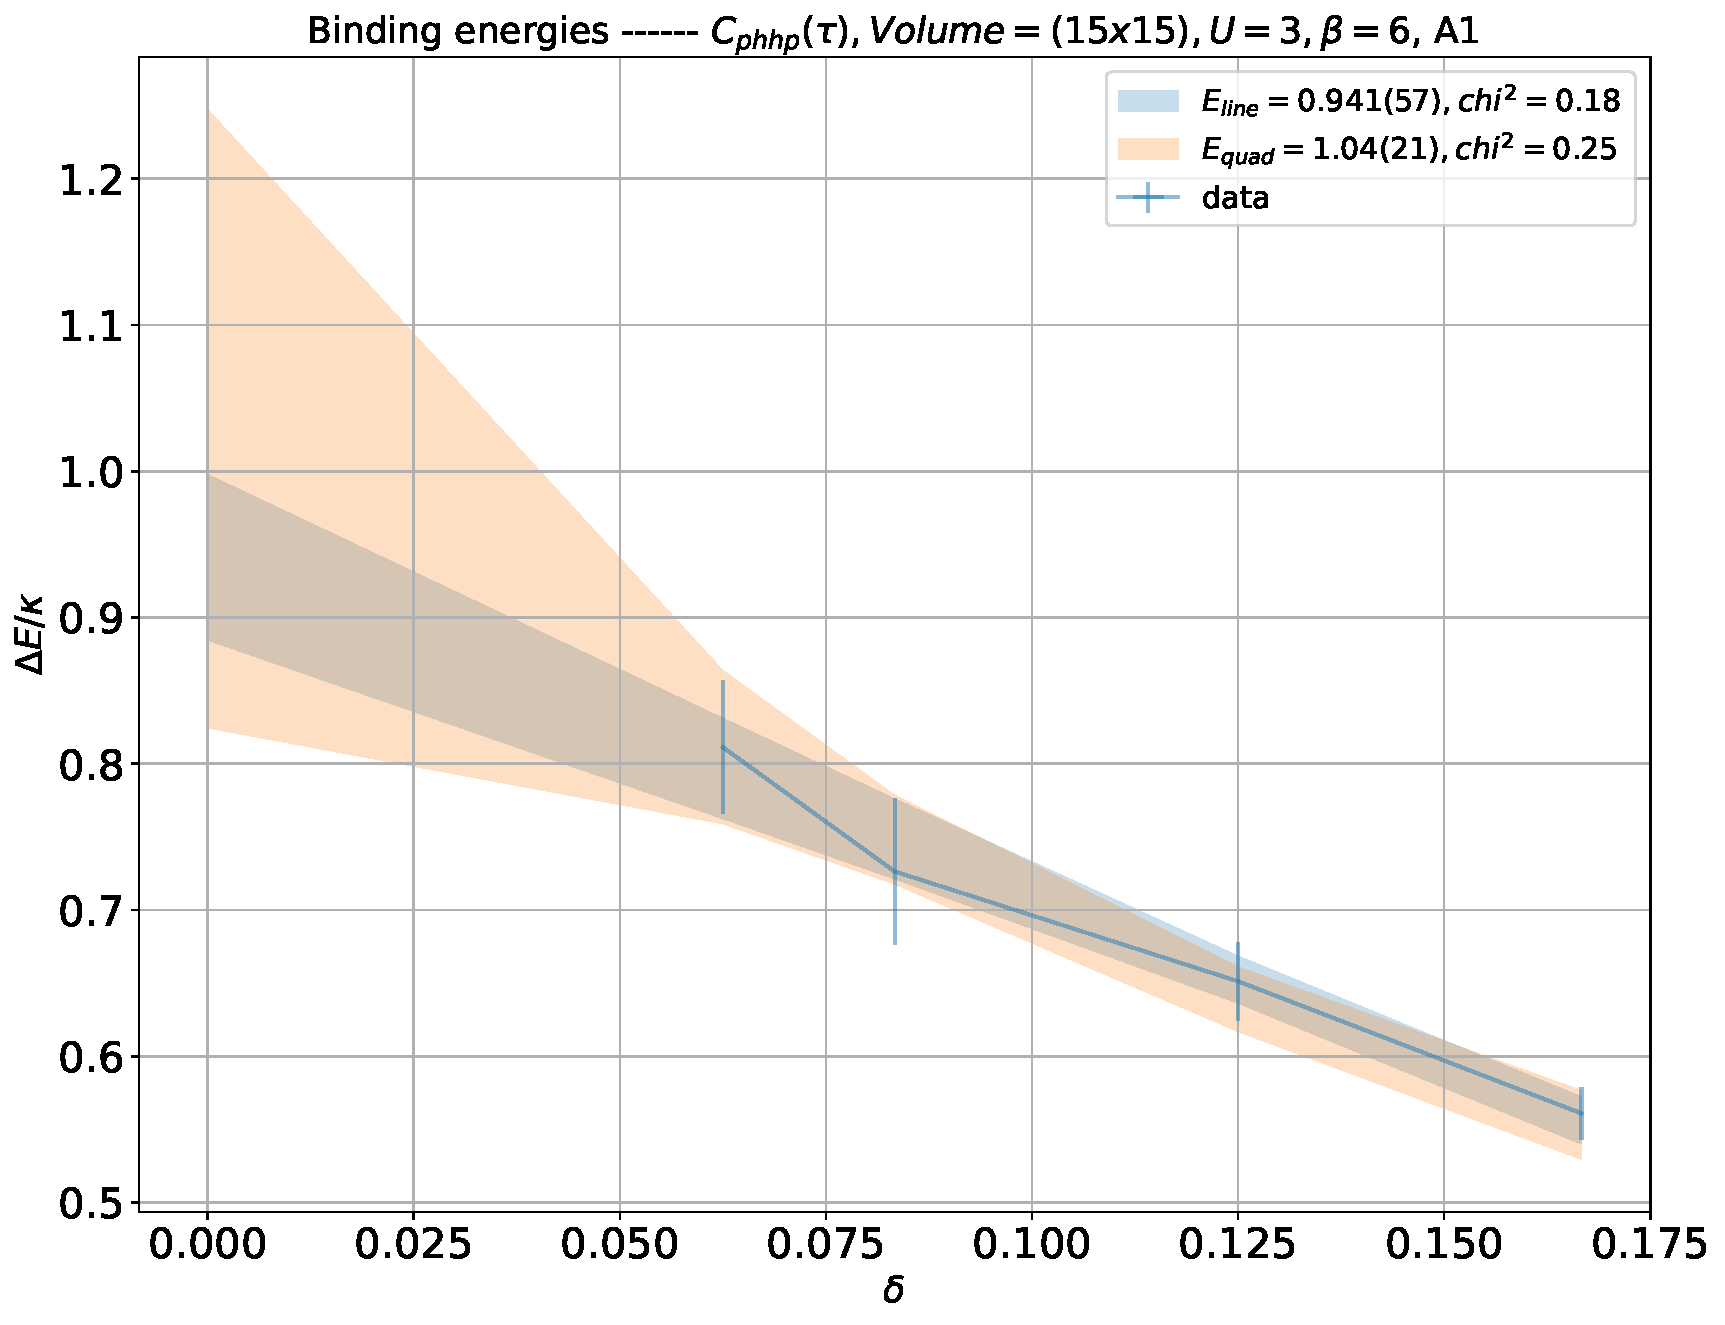
\includegraphics[width=\linewidth]{phhp-0-A1_15x15_U3_B6_cont.pdf}
  \end{subfigure}
  \begin{subfigure}{.5\textwidth}
      \centering
      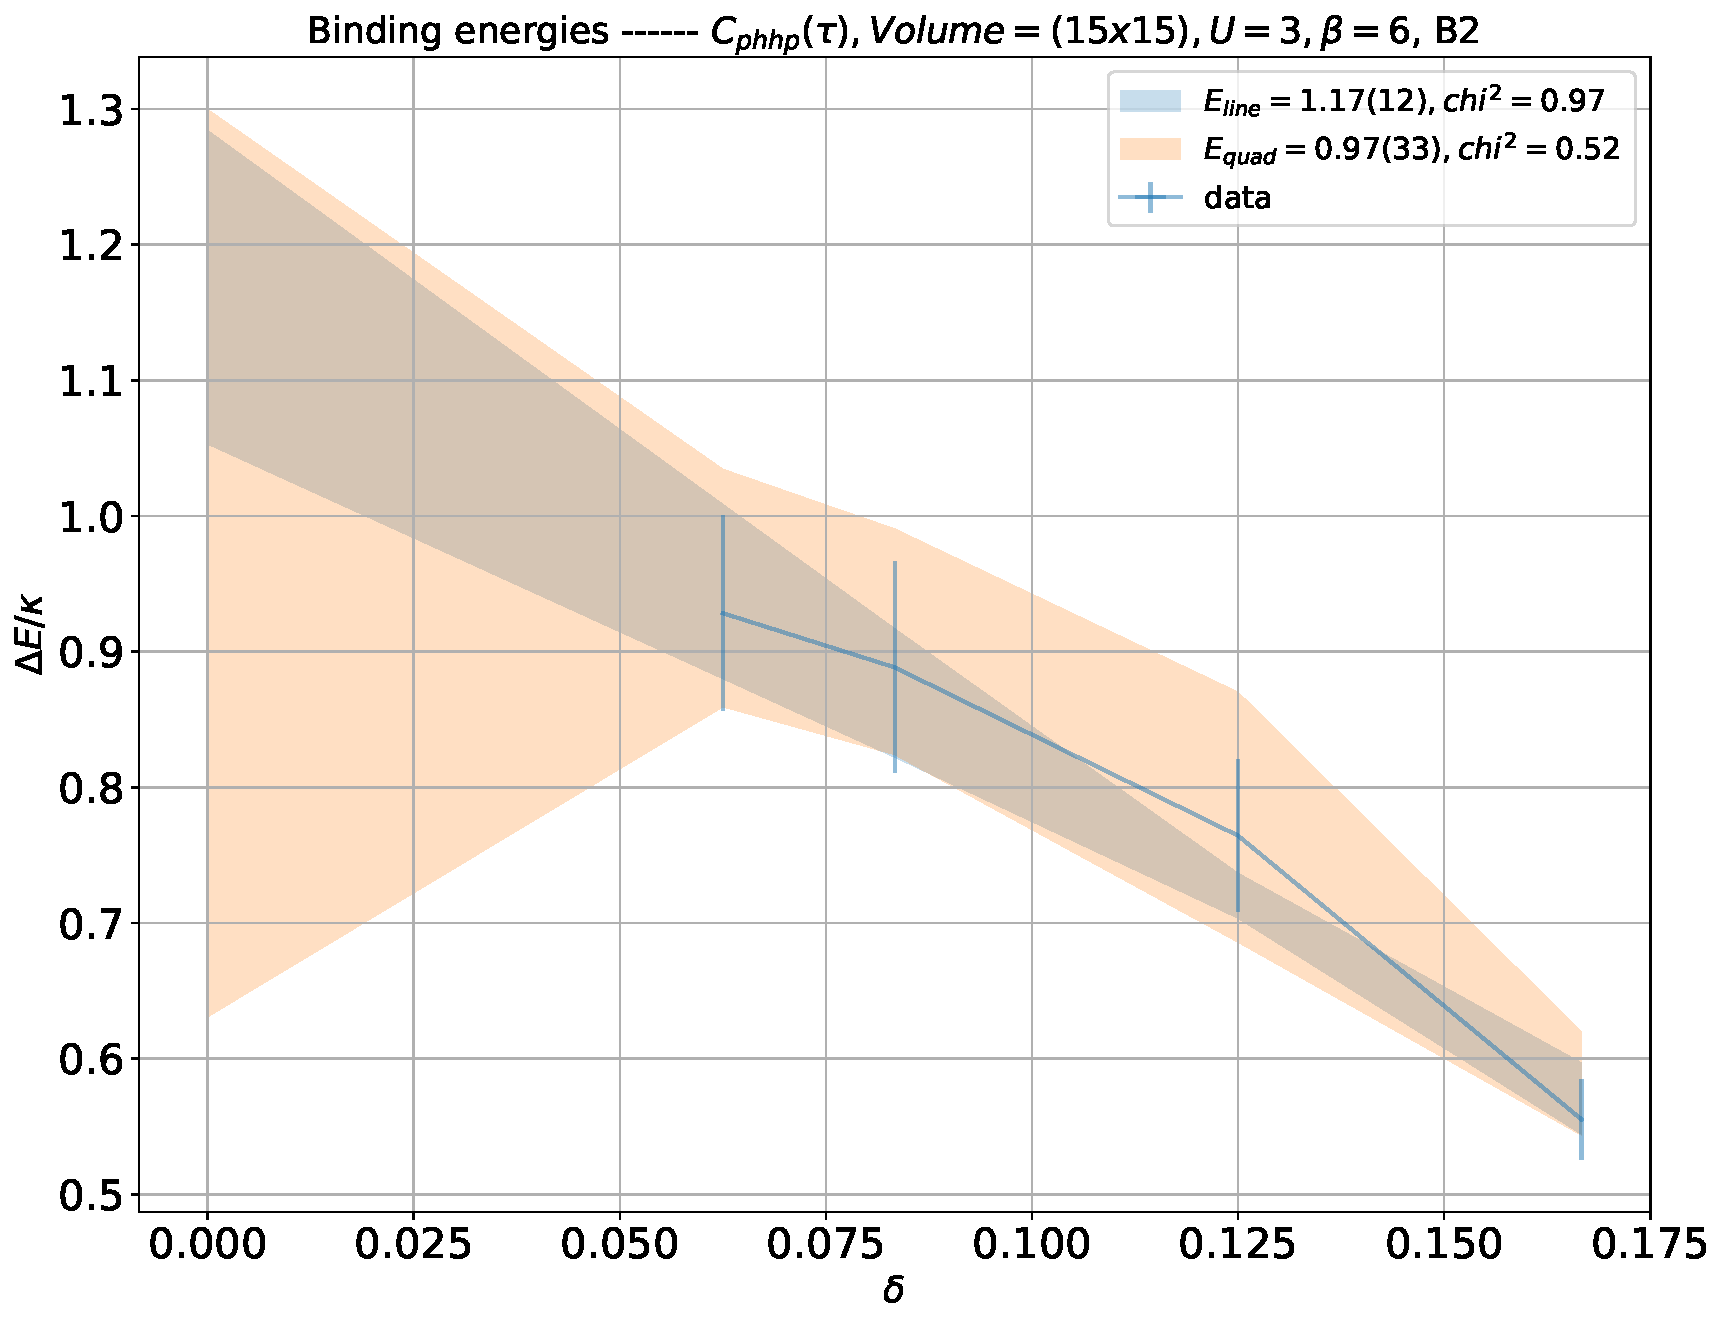
\includegraphics[width=\linewidth]{phhp-0-B2_15x15_U3_B6_cont.pdf}
  \end{subfigure}
  \caption{Binding energy extraction of the particle-hole pair at both irreducible representations, where we fit one- and two-body correlators for every $N_t$. This is followed by fitting a linear and a quadratic functions to the $\Delta E_{N_t}$ in order to extrapolate to the continuum limit ($N_t\to\infty$).}
  \label{fig:fig4}
\end{figure}

\begin{figure}
  \begin{subfigure}{.5\textwidth}
    \centering
    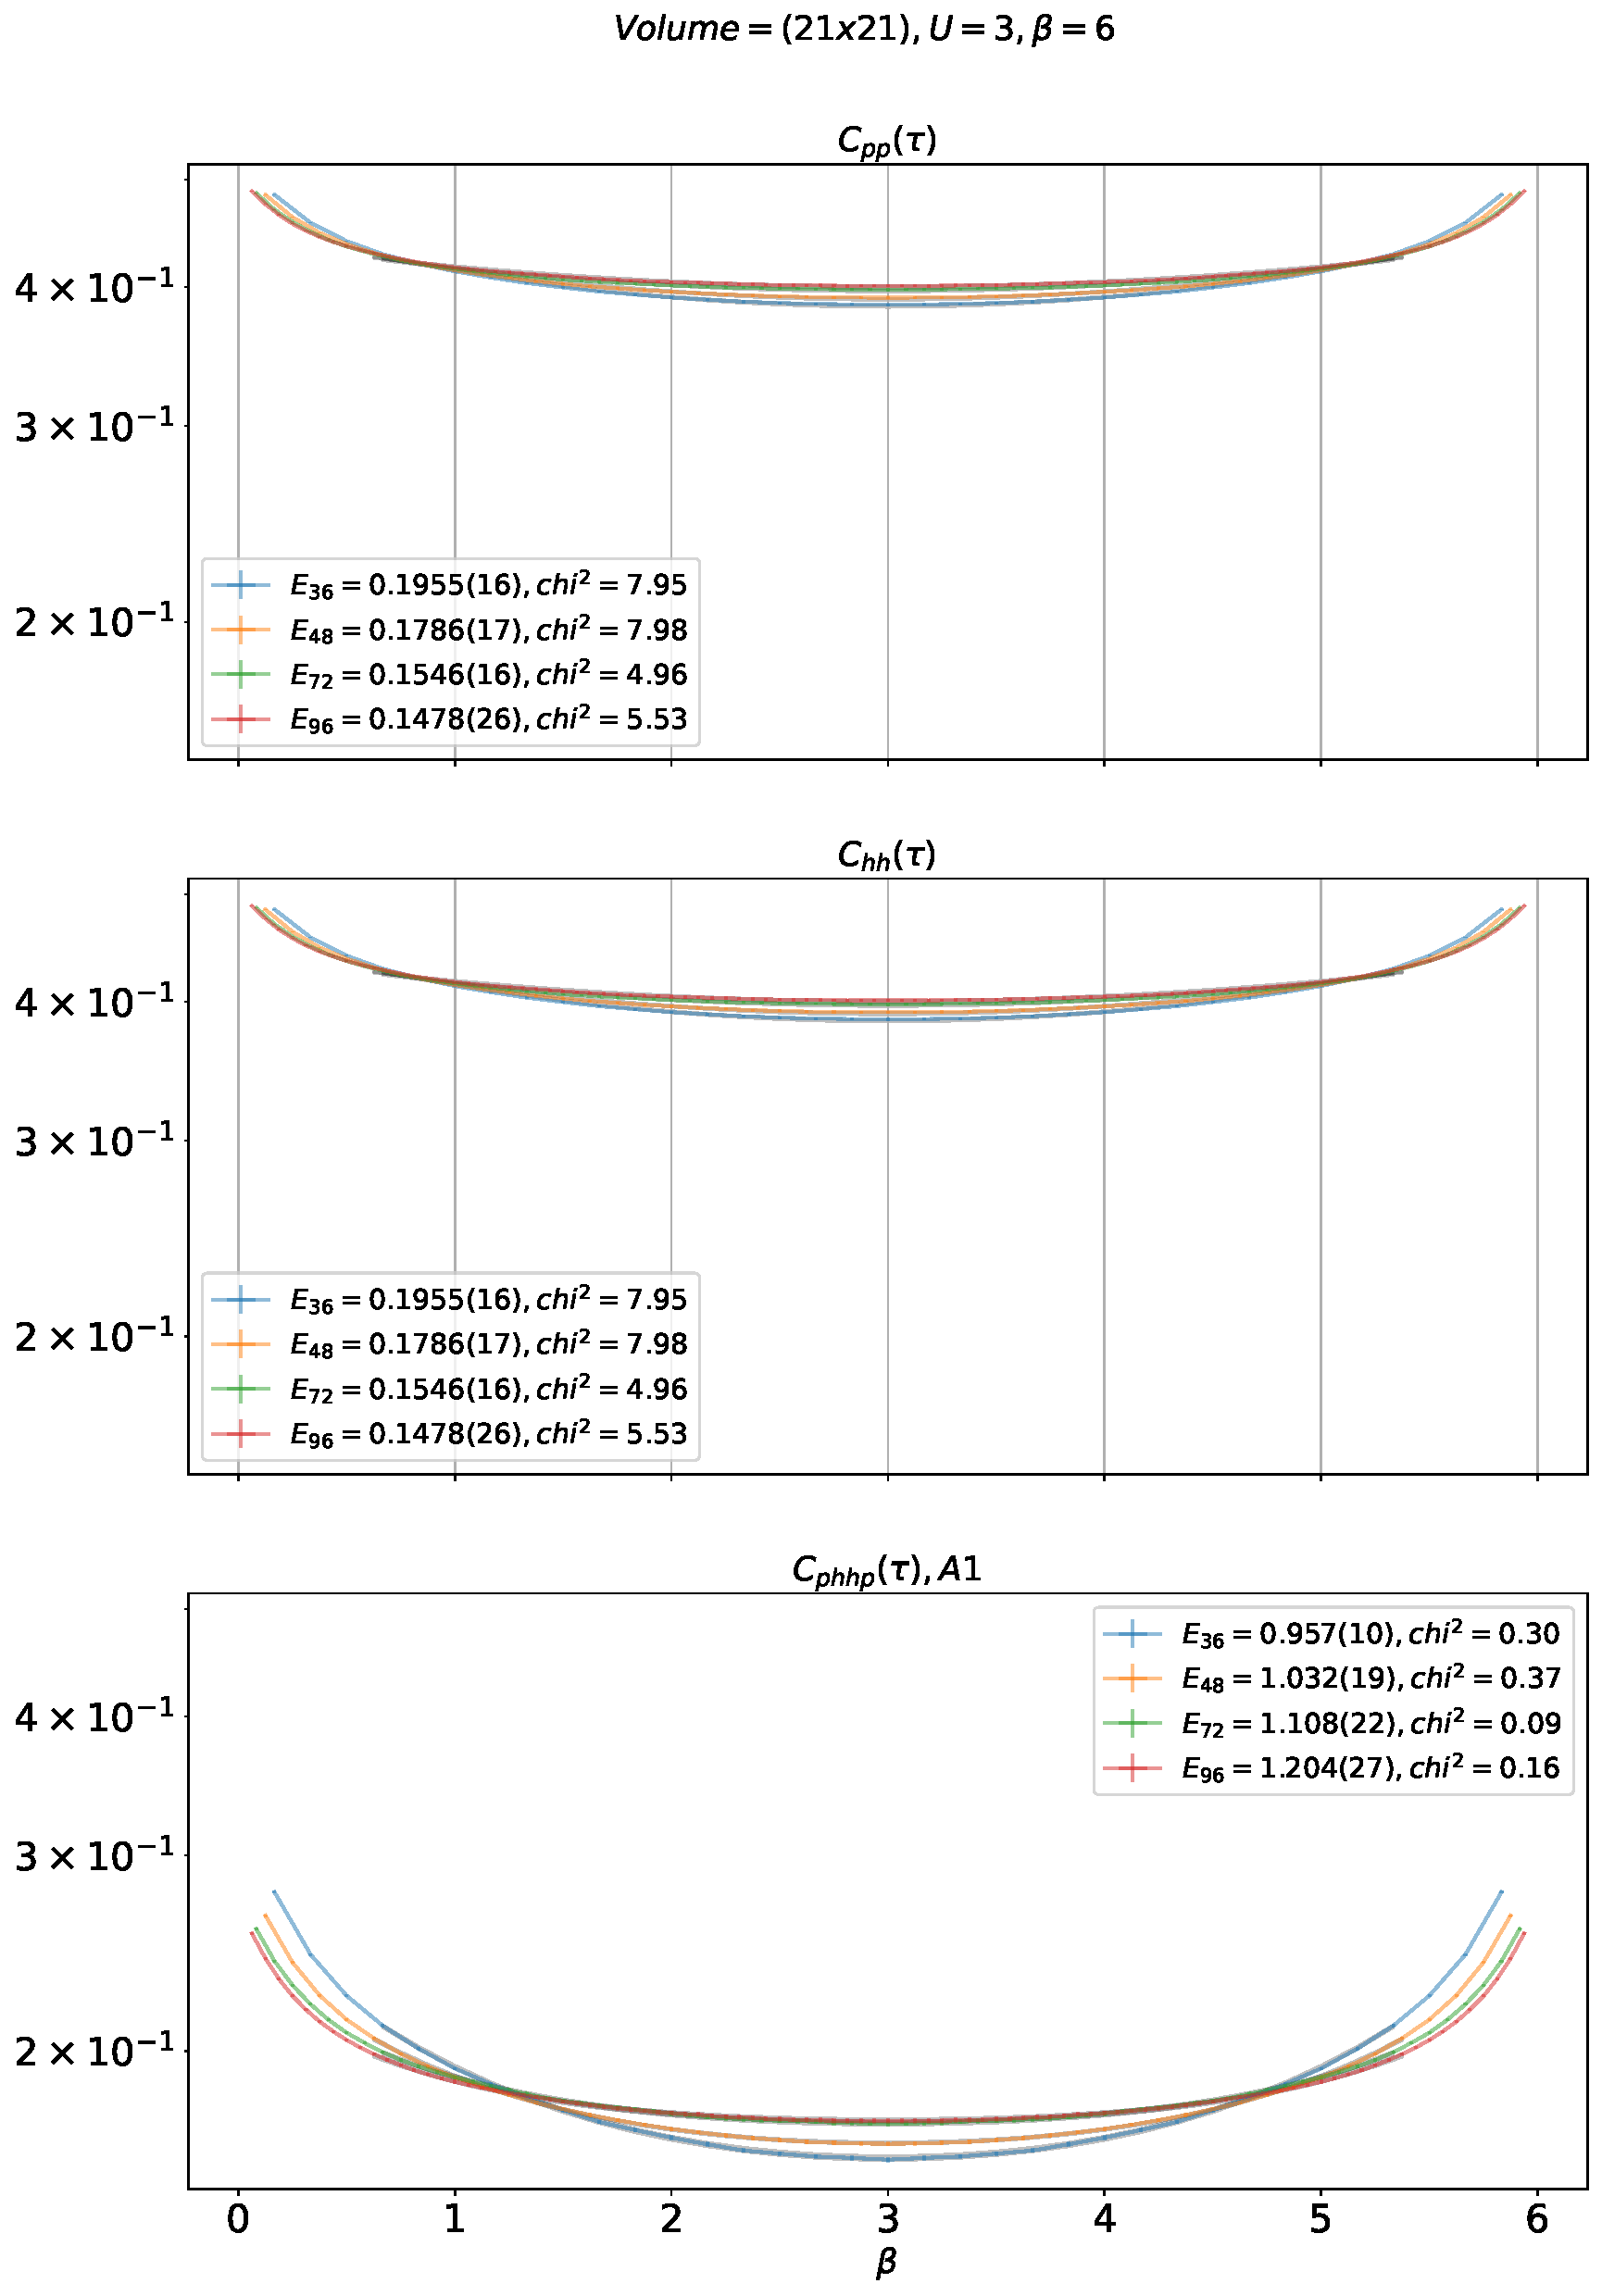
\includegraphics[width=\linewidth]{phhp-0-A1_21x21_U3_B6.pdf}
  \end{subfigure}%
  \begin{subfigure}{.5\textwidth}
    \centering
    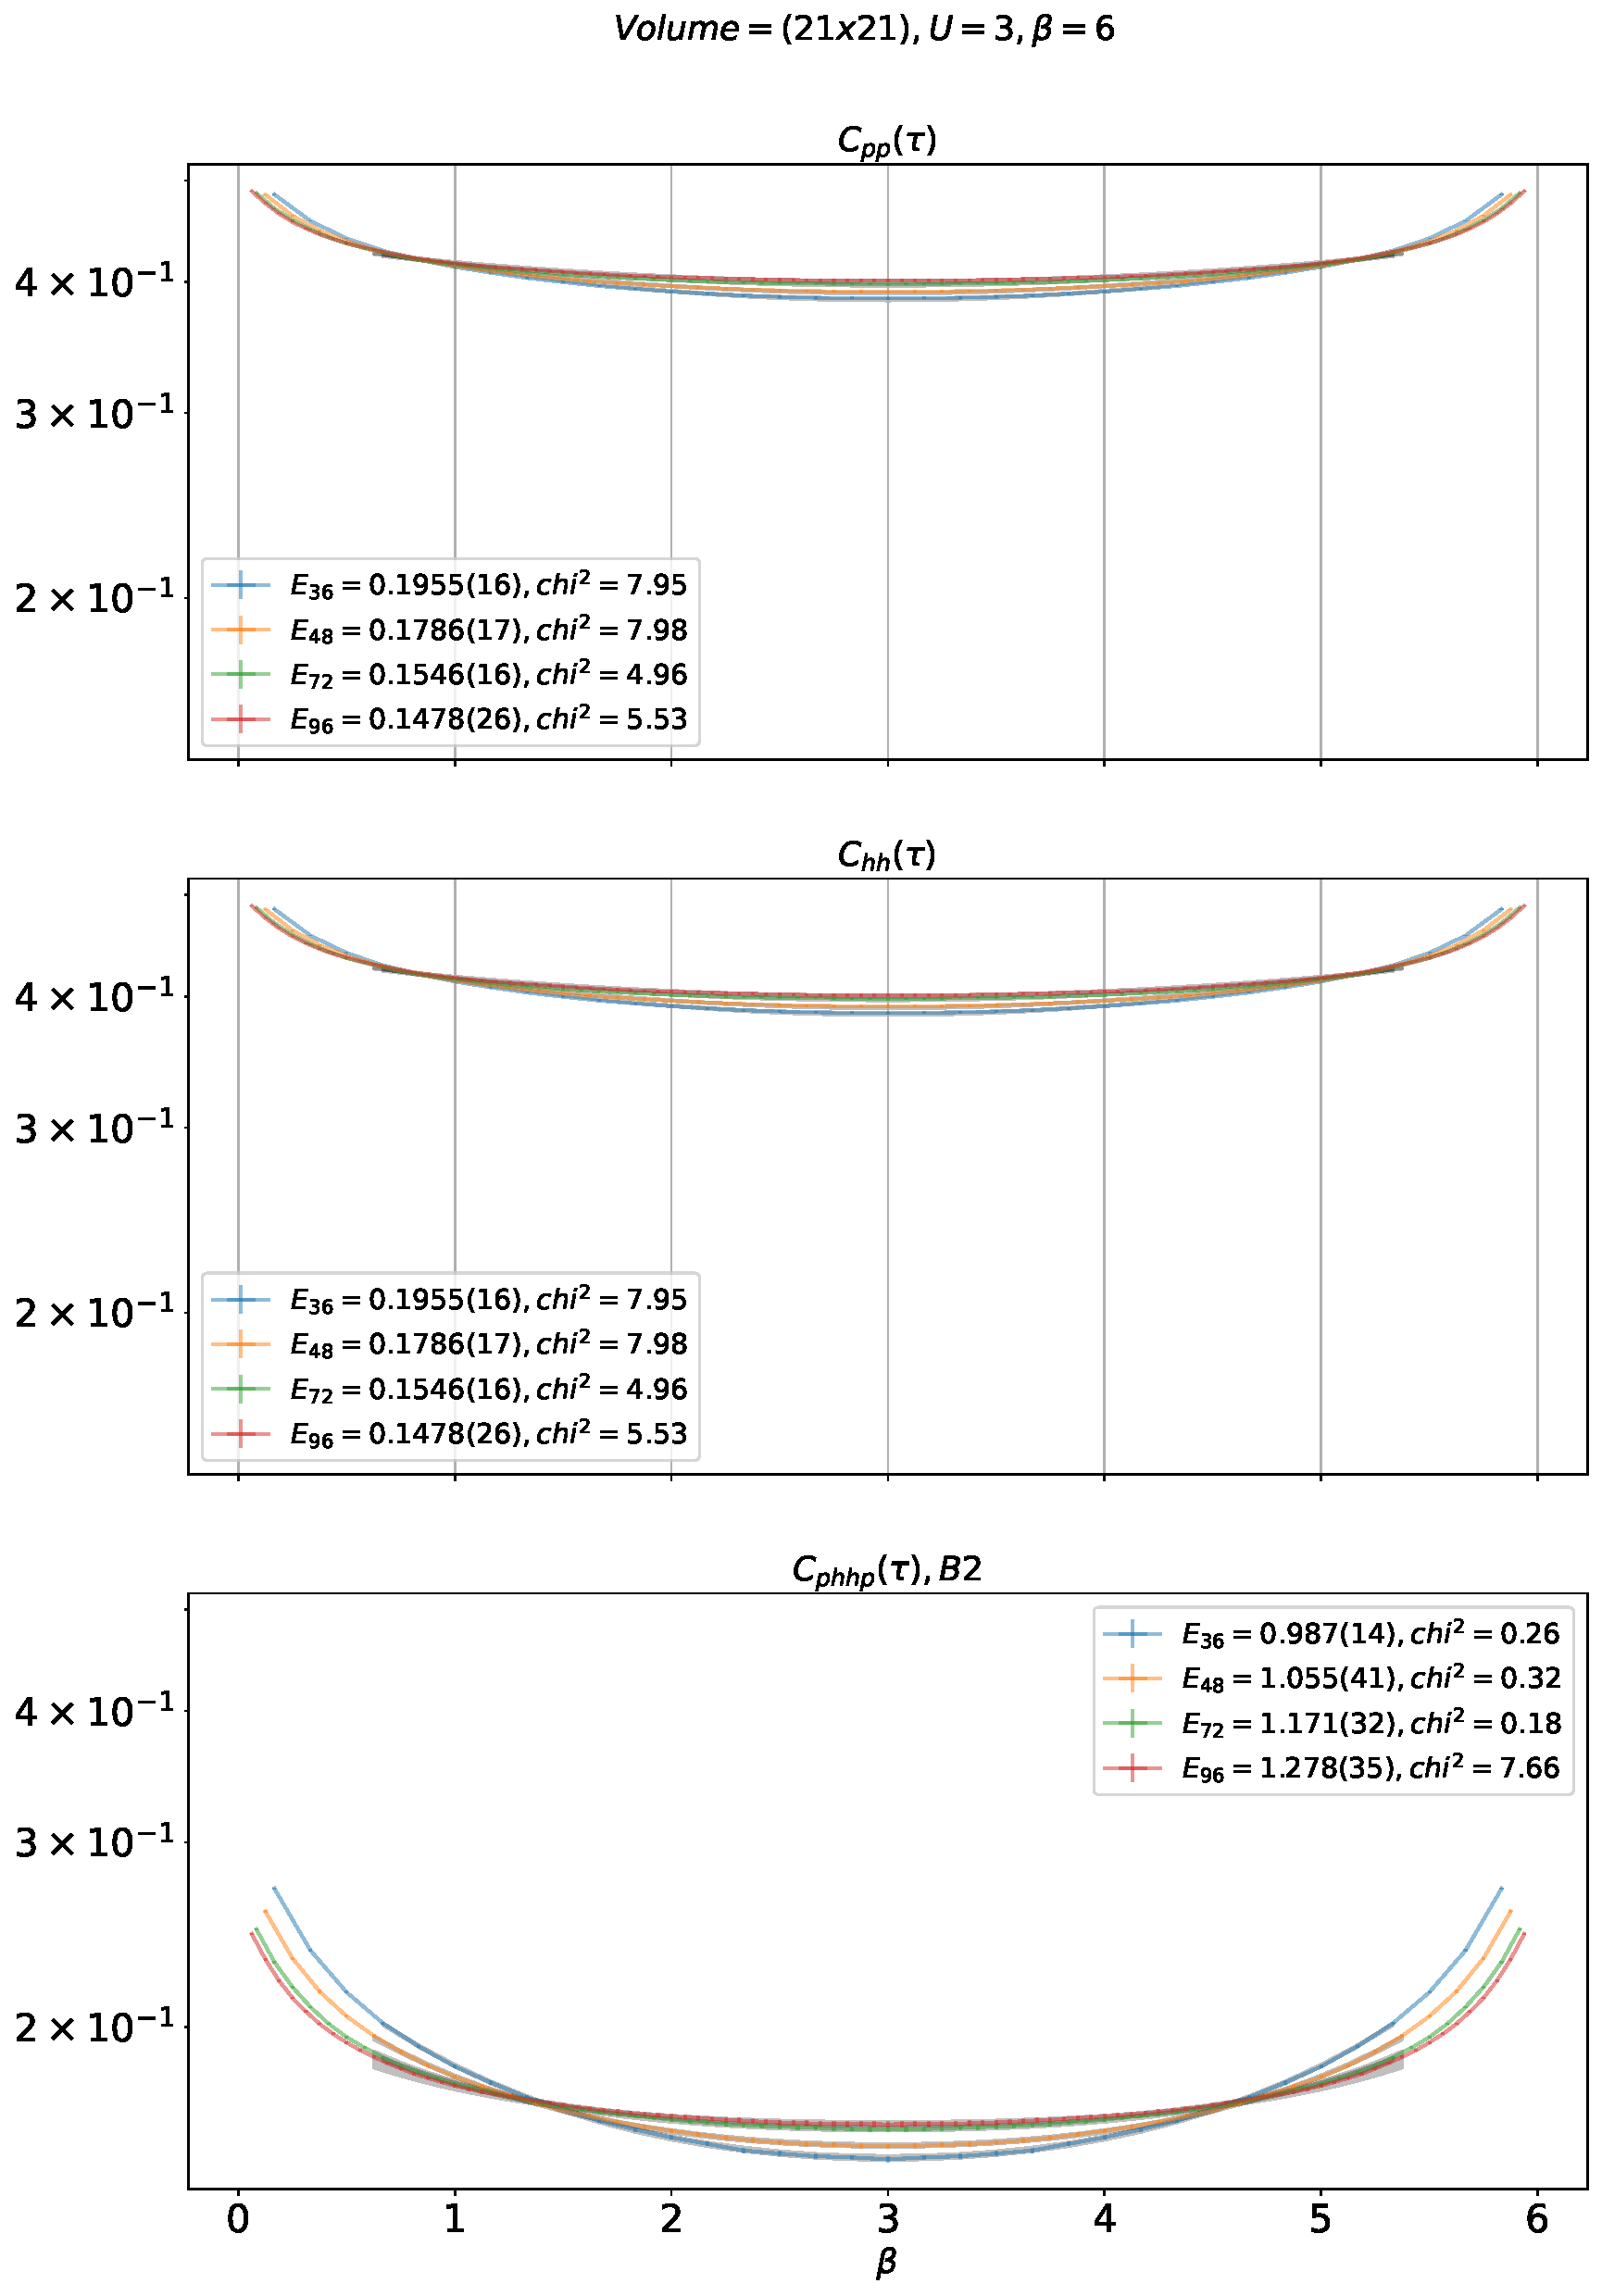
\includegraphics[width=\linewidth]{phhp-0-B2_21x21_U3_B6.pdf}
  \end{subfigure}
  \begin{subfigure}{.5\textwidth}
      \centering
      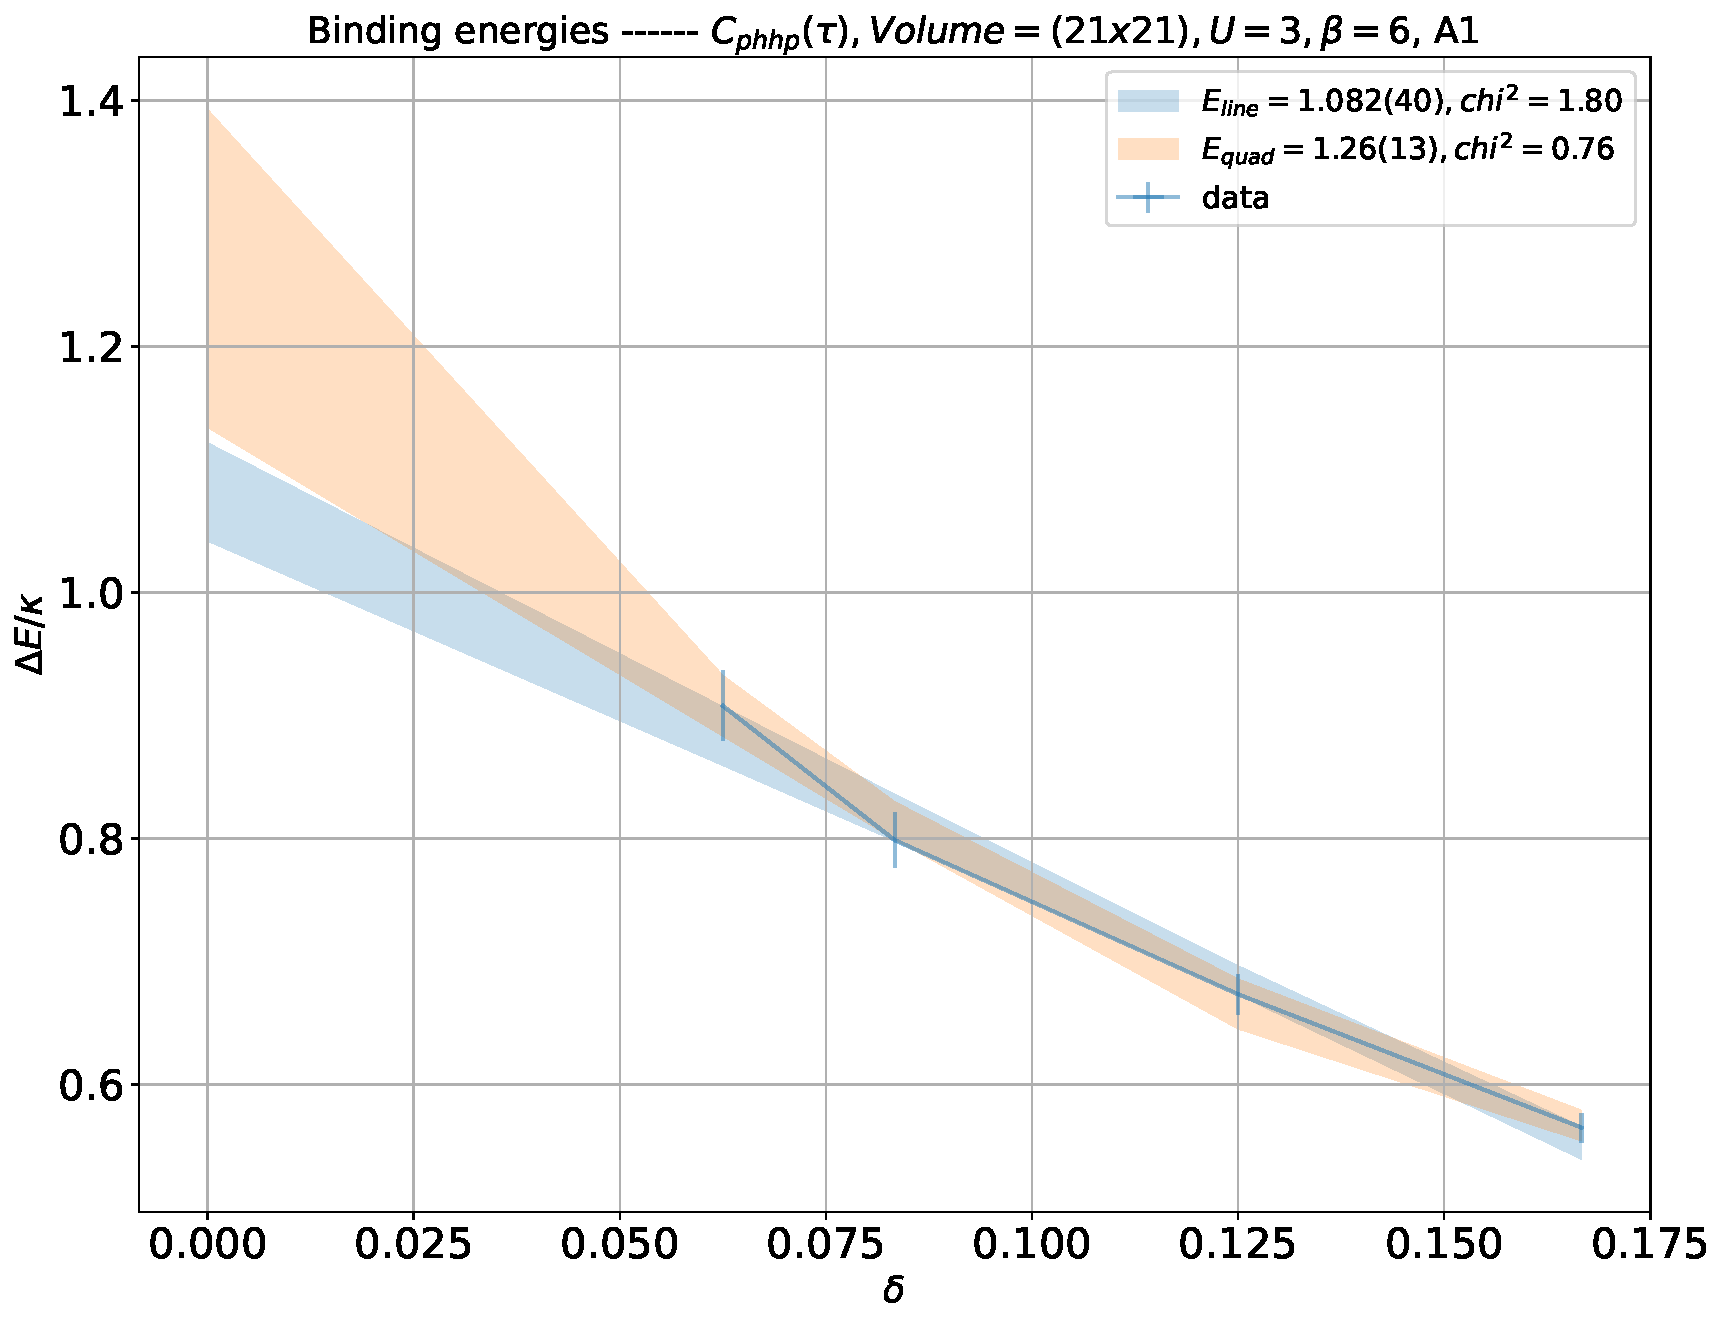
\includegraphics[width=\linewidth]{phhp-0-A1_21x21_U3_B6_cont.pdf}
  \end{subfigure}
  \begin{subfigure}{.5\textwidth}
      \centering
      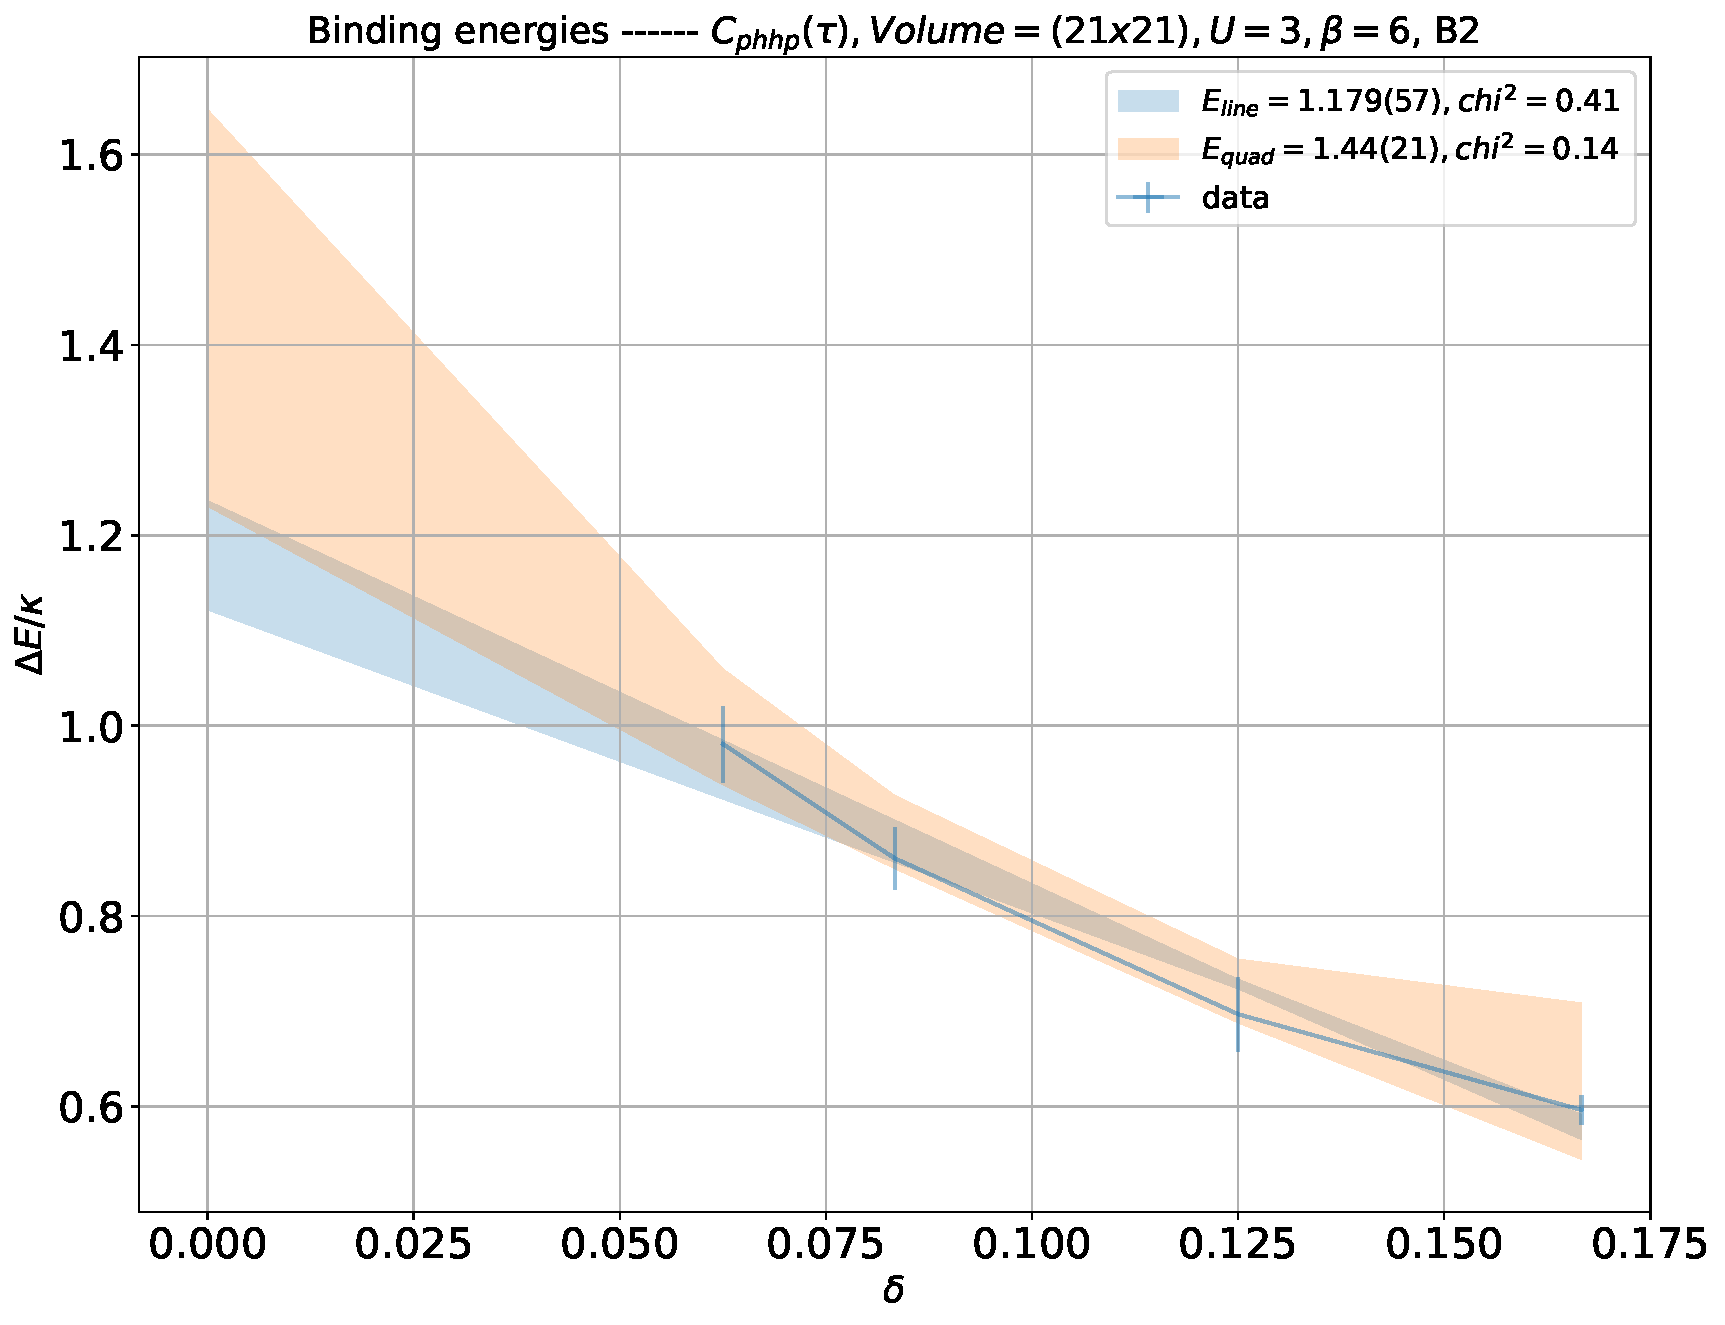
\includegraphics[width=\linewidth]{phhp-0-B2_21x21_U3_B6_cont.pdf}
  \end{subfigure}
  \caption{Binding energy extraction of the particle-hole pair at both irreducible representations, where we fit one- and two-body correlators for every $N_t$. This is followed by fitting a linear and a quadratic functions to the $\Delta E_{N_t}$ in order to extrapolate to the continuum limit ($N_t\to\infty$).}
  \label{fig:fig5}
\end{figure}

\begin{figure}
  \begin{subfigure}{.5\textwidth}
    \centering
    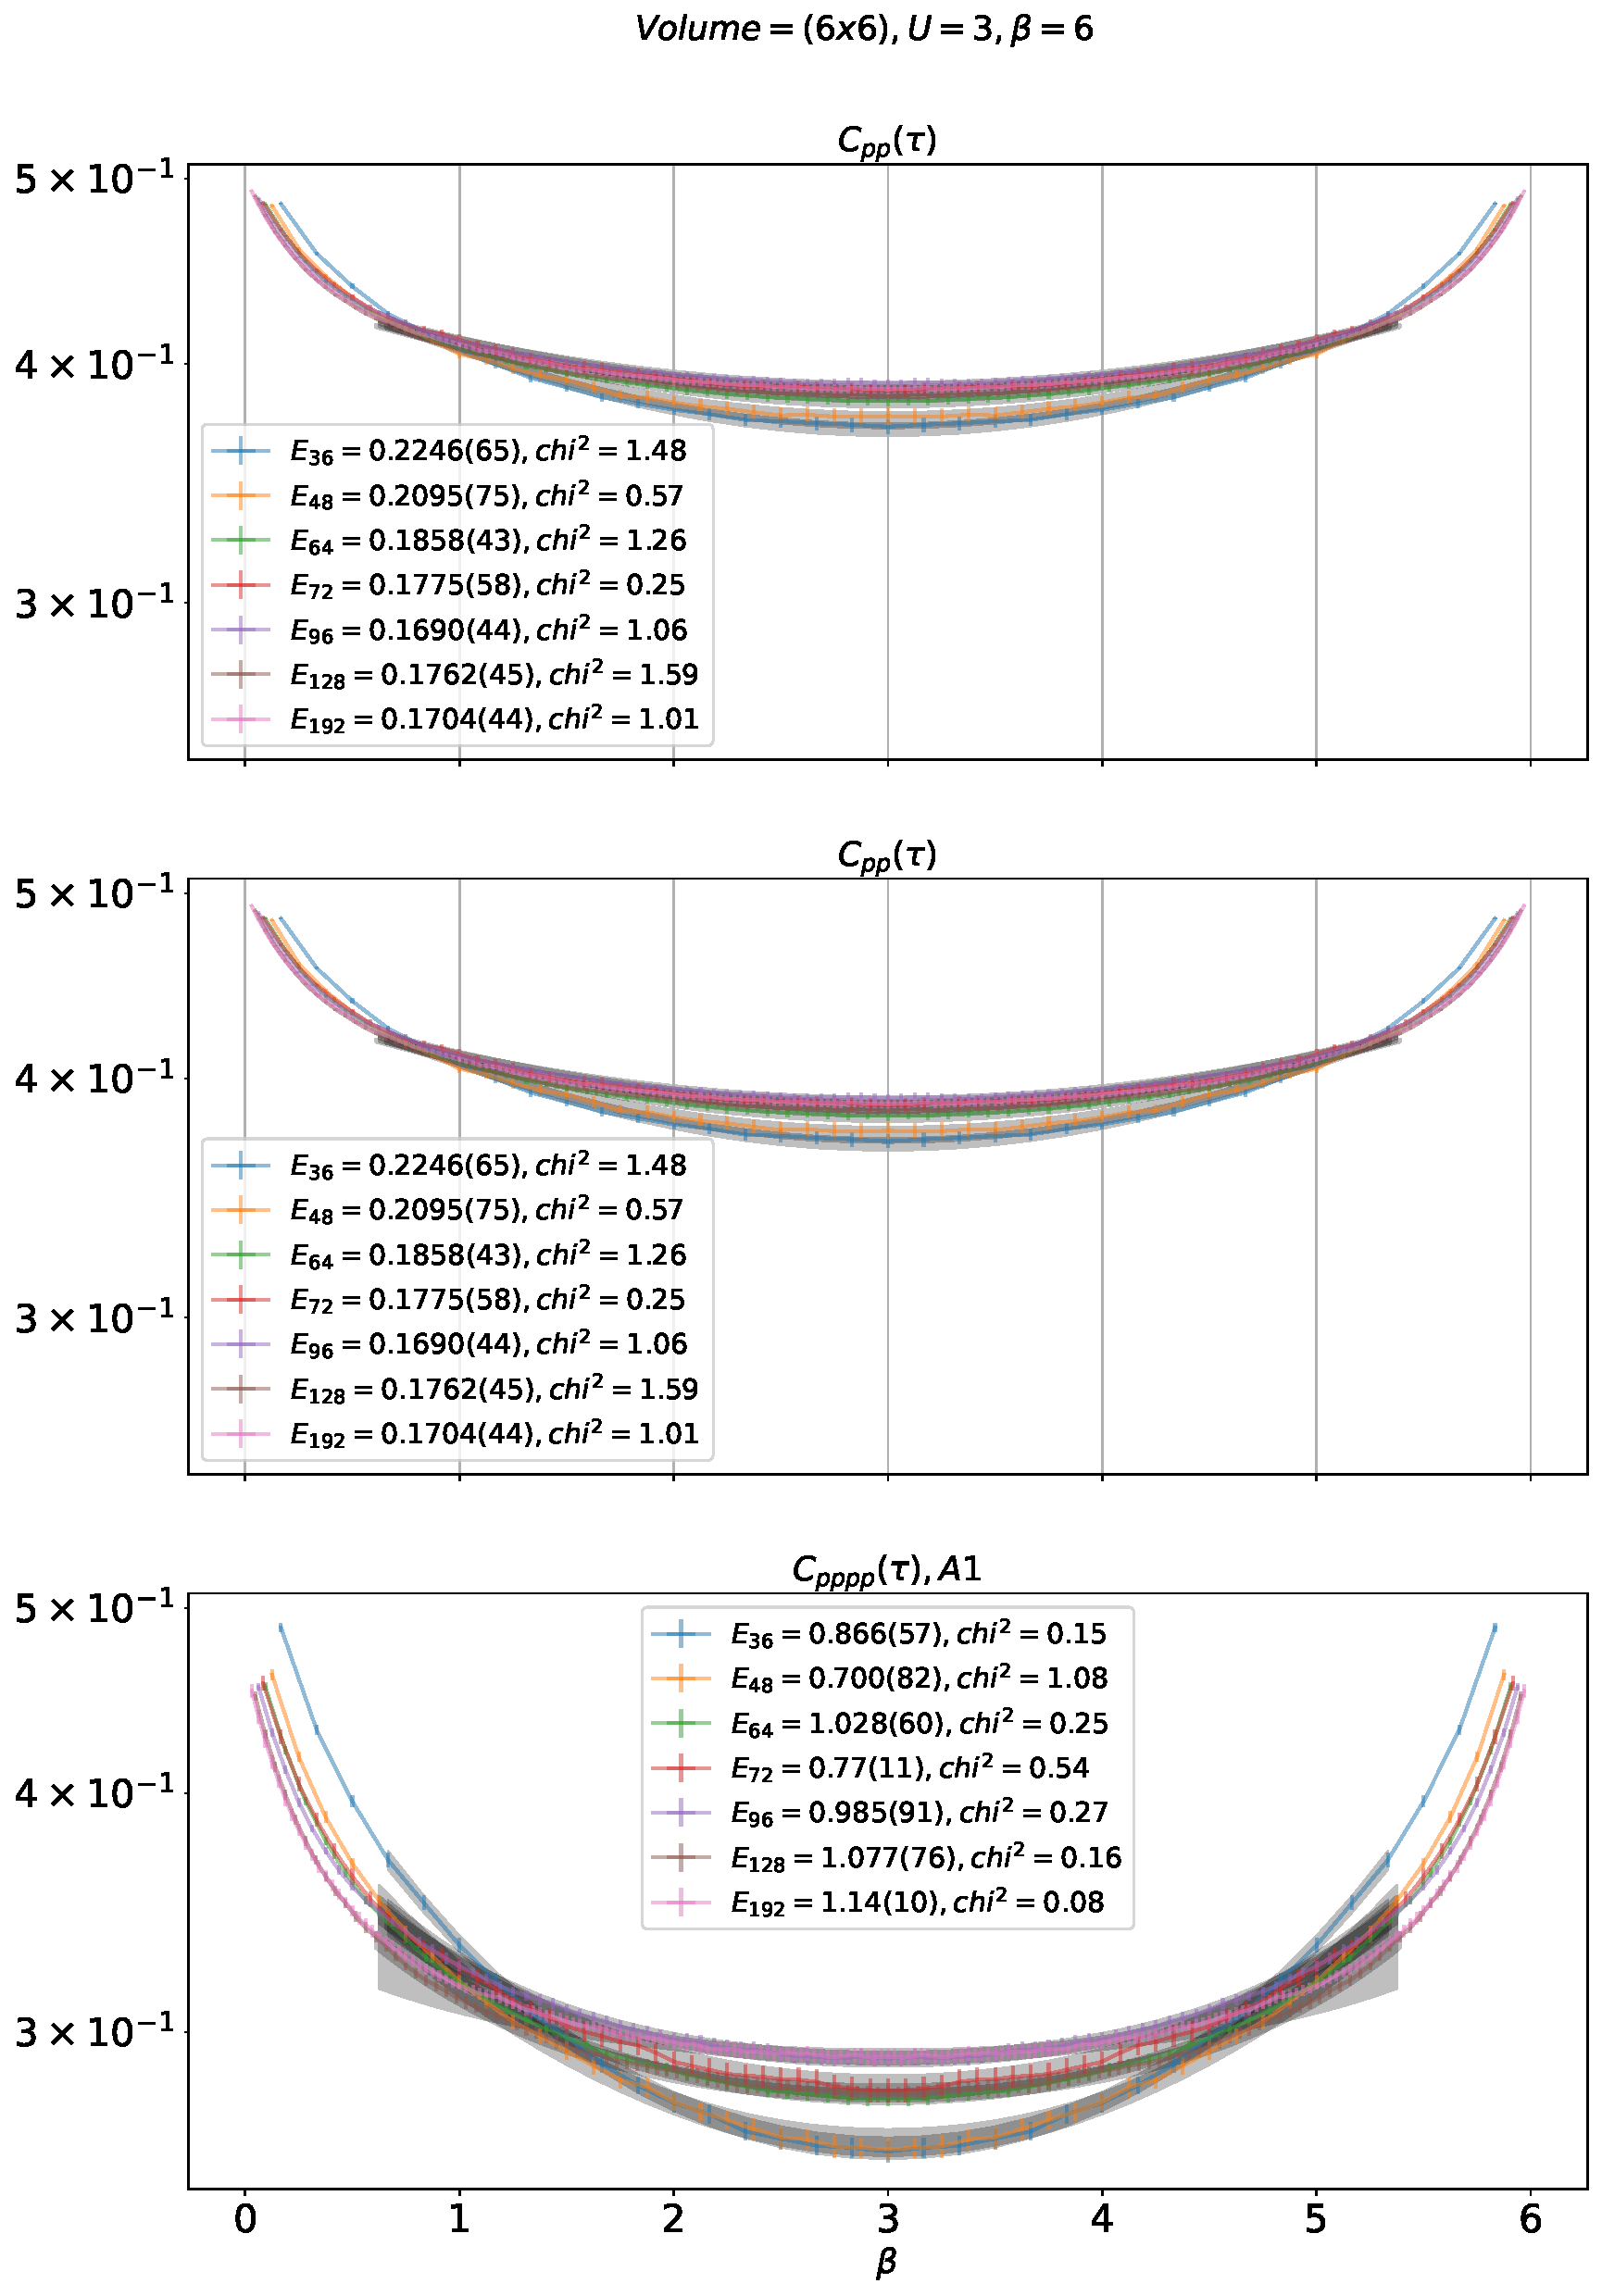
\includegraphics[width=\linewidth]{pppp-0-A1_6x6_U3.0_B6.0.pdf}
  \end{subfigure}%
  \begin{subfigure}{.5\textwidth}
    \centering
    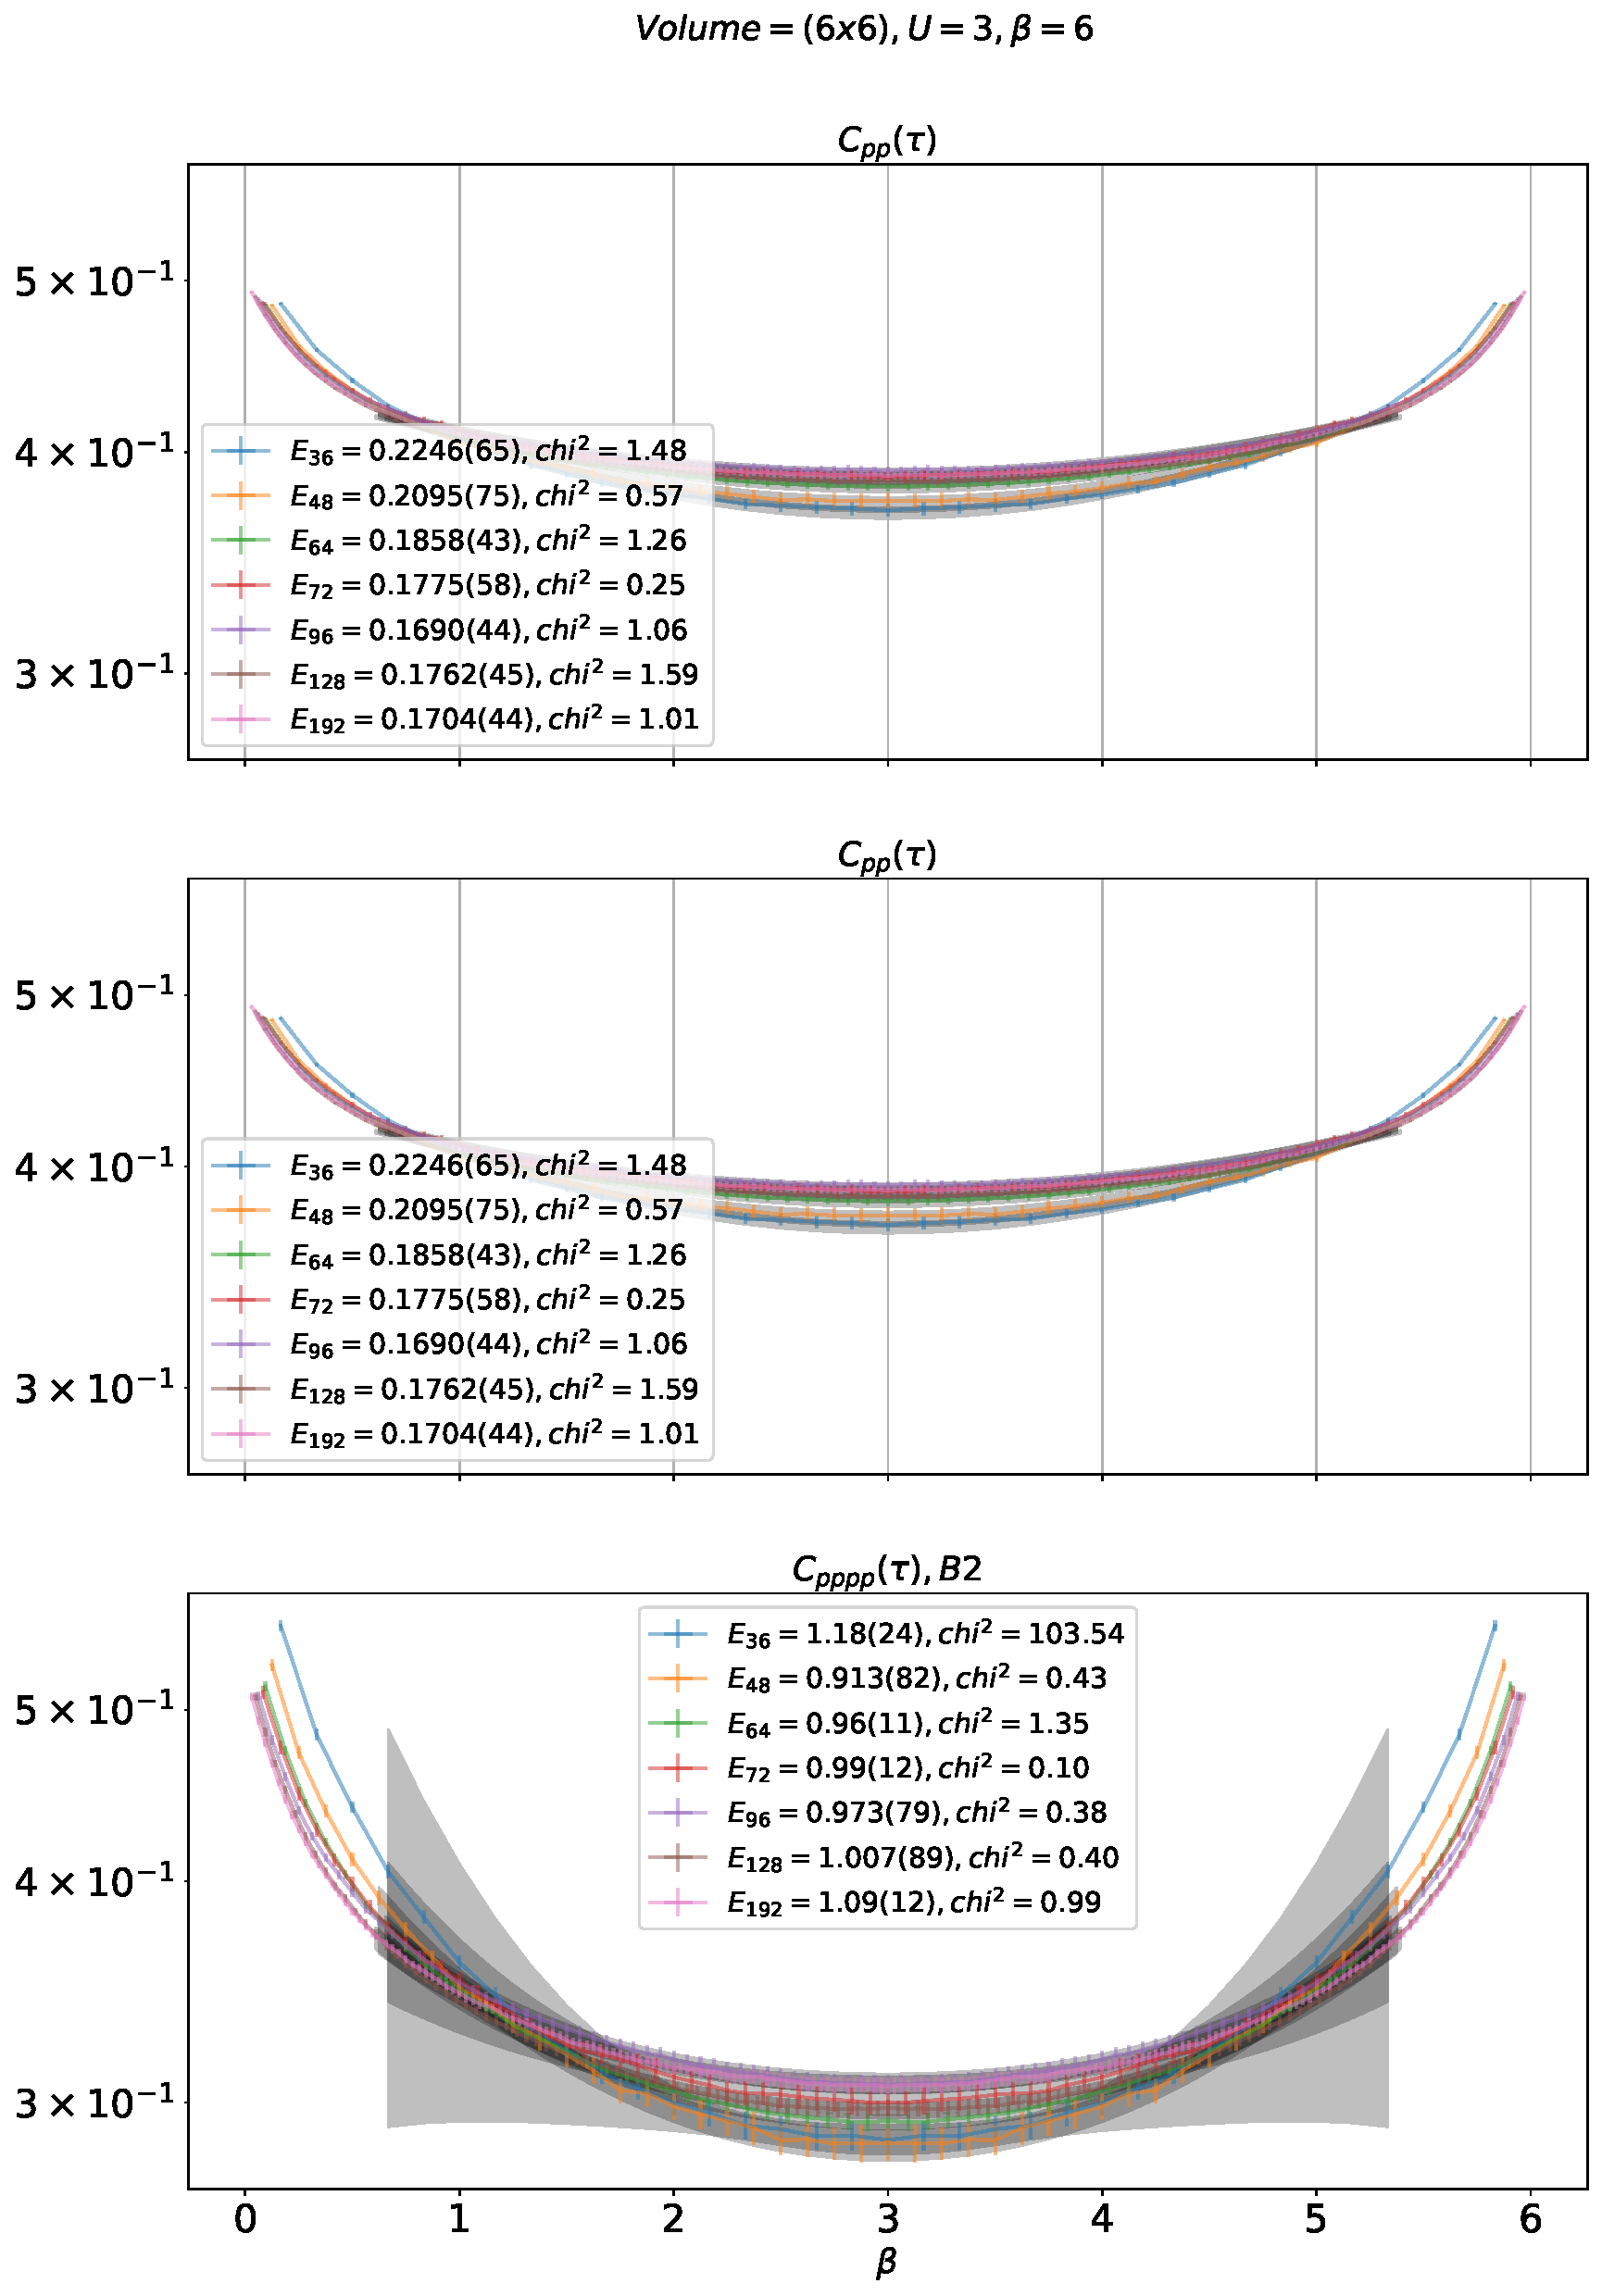
\includegraphics[width=\linewidth]{pppp-0-B2_6x6_U3.0_B6.0.pdf}
  \end{subfigure}
  \begin{subfigure}{.5\textwidth}
      \centering
      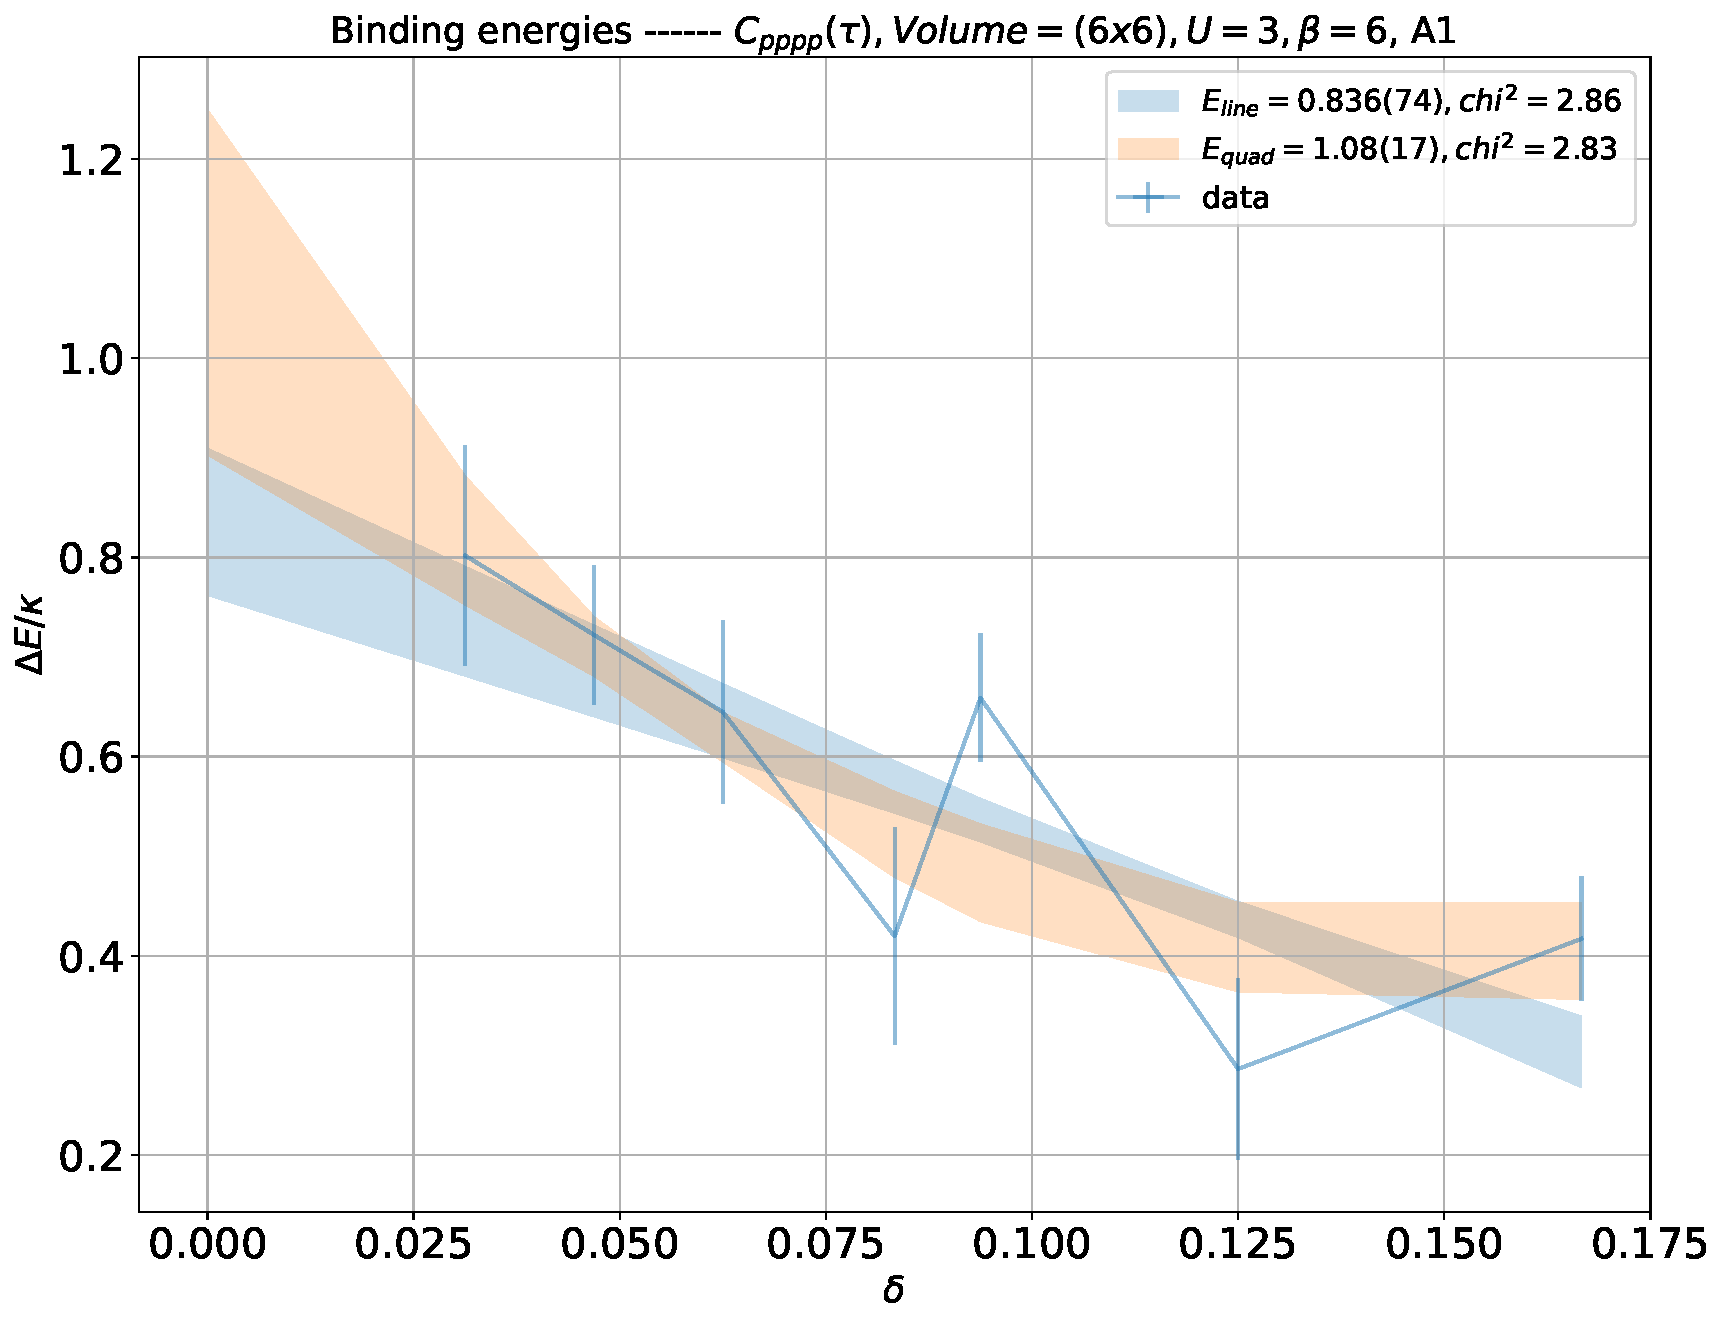
\includegraphics[width=\linewidth]{pppp-0-A1_6x6_U3.0_B6.0_cont.pdf}
  \end{subfigure}
  \begin{subfigure}{.5\textwidth}
      \centering
      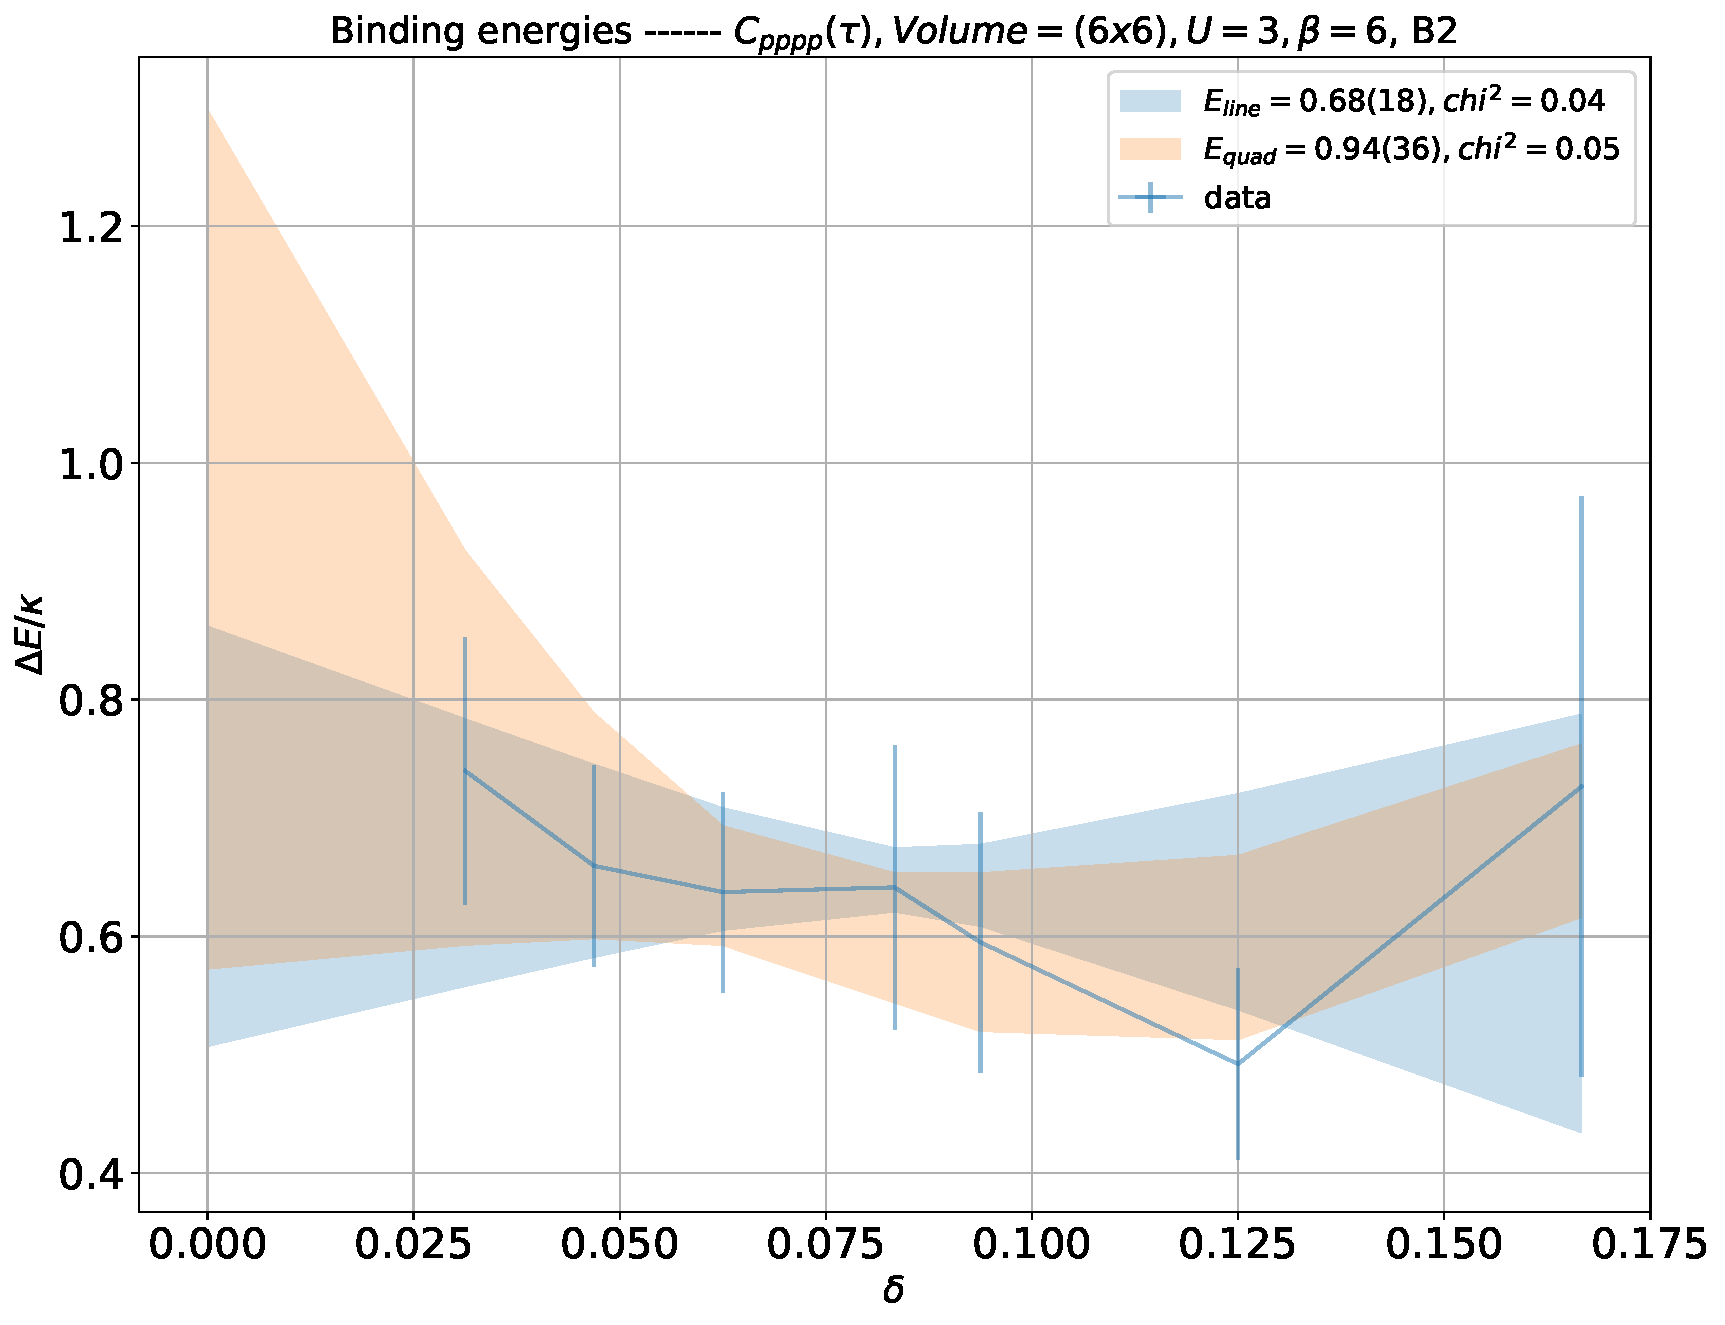
\includegraphics[width=\linewidth]{pppp-0-B2_6x6_U3.0_B6.0_cont.pdf}
  \end{subfigure}
  \caption{Binding energy extraction of the particle-particle pair at both irreducible representations, where we fit one- and two-body correlators for every $N_t$. This is followed by fitting a linear and a quadratic functions to the $\Delta E_{N_t}$ in order to extrapolate to the continuum limit ($N_t\to\infty$).}
  \label{fig:fig6}
\end{figure}

\begin{figure}
  \begin{subfigure}{.5\textwidth}
    \centering
    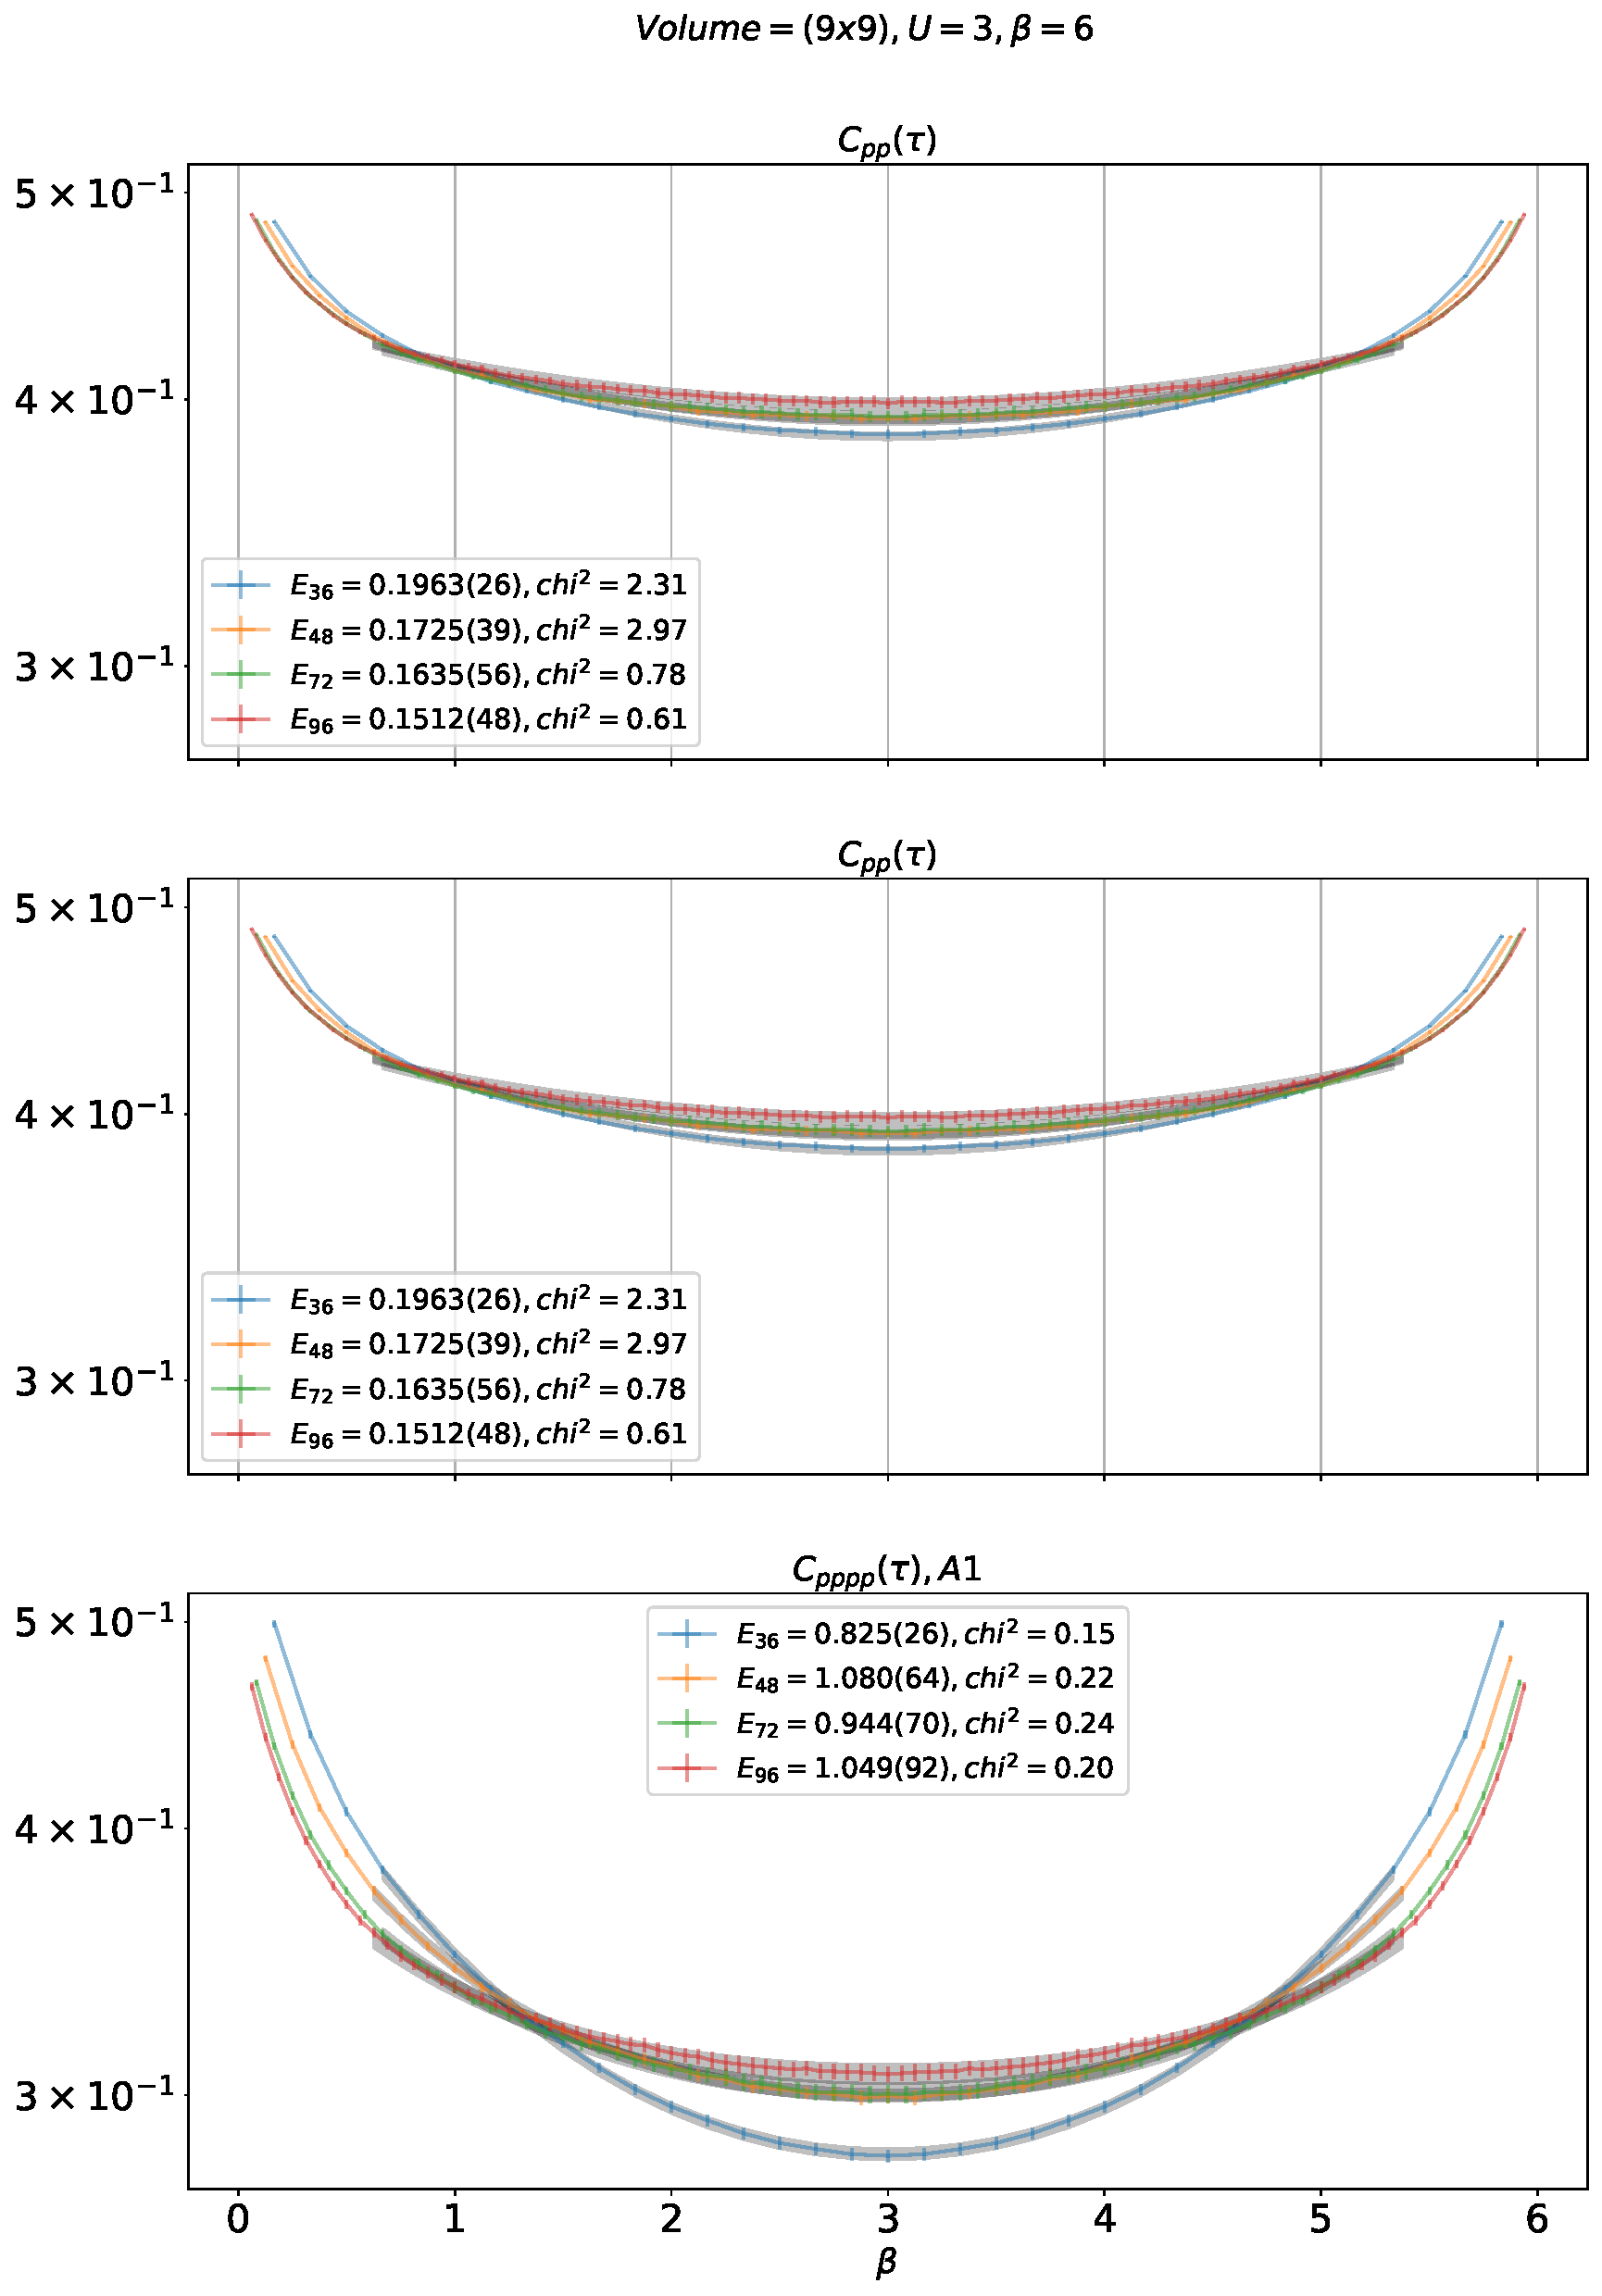
\includegraphics[width=\linewidth]{pppp-0-A1_9x9_U3_B6.pdf}
  \end{subfigure}%
  \begin{subfigure}{.5\textwidth}
    \centering
    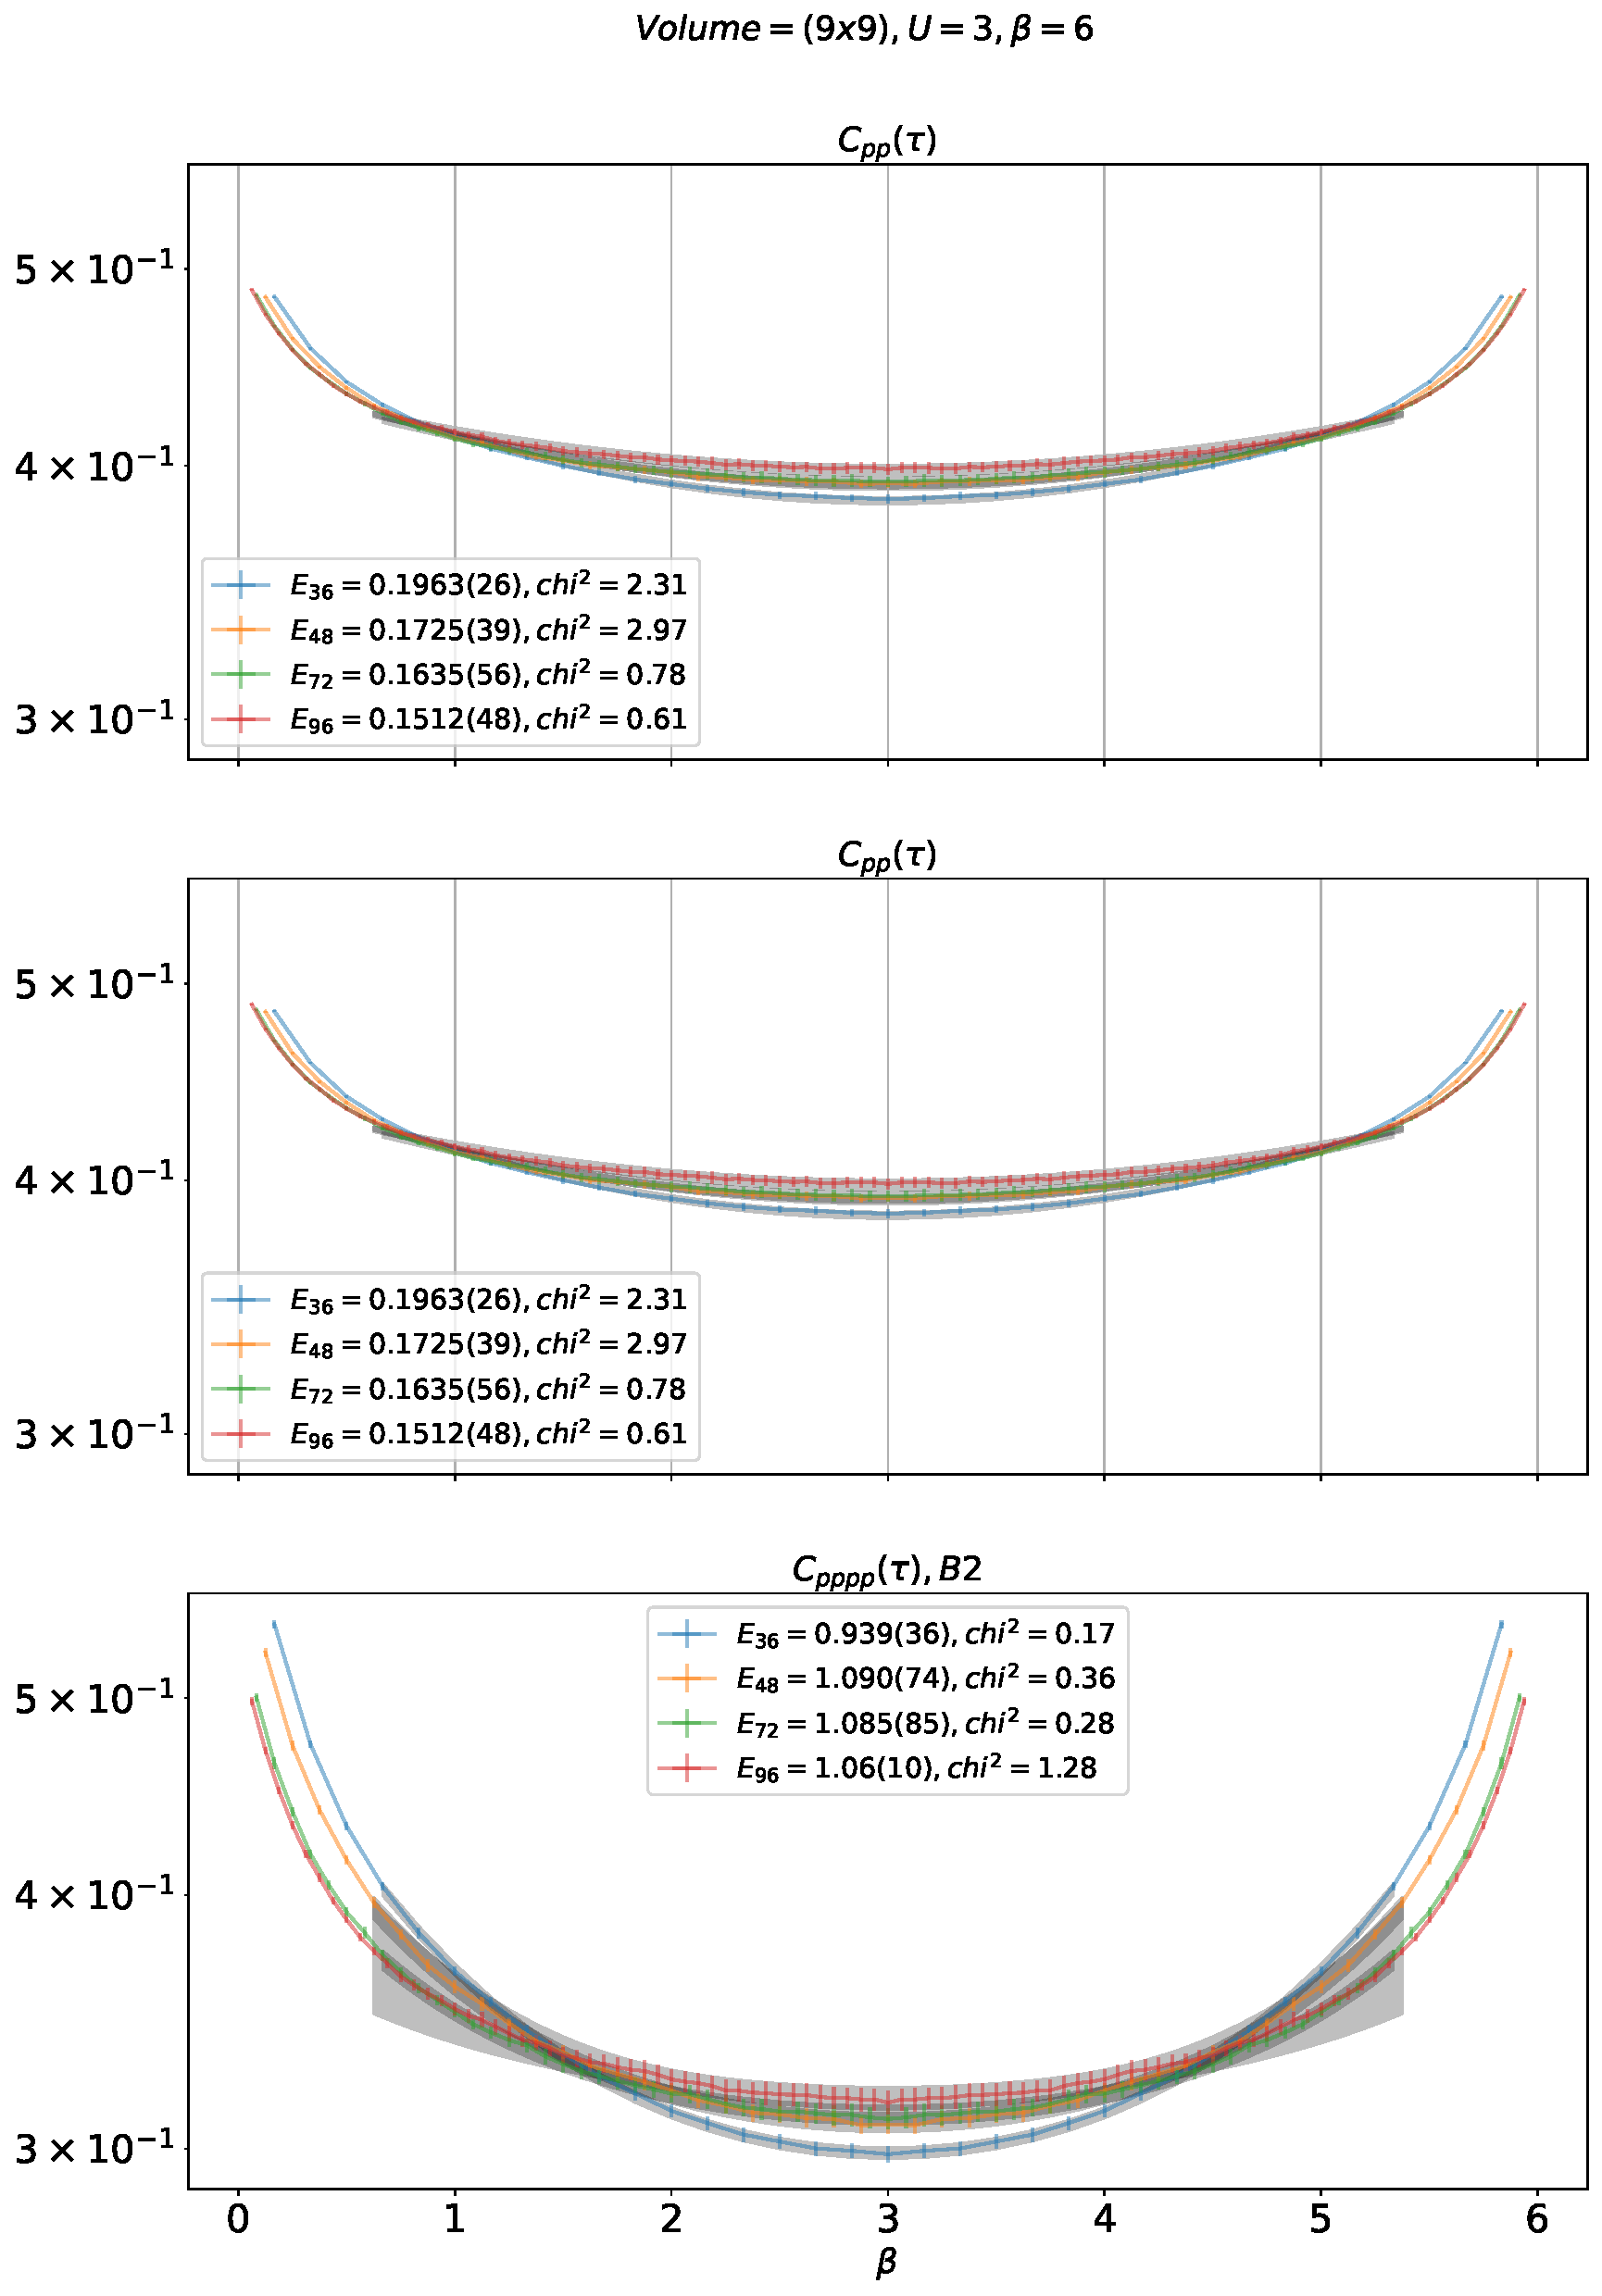
\includegraphics[width=\linewidth]{pppp-0-B2_9x9_U3_B6.pdf}
  \end{subfigure}
  \begin{subfigure}{.5\textwidth}
      \centering
      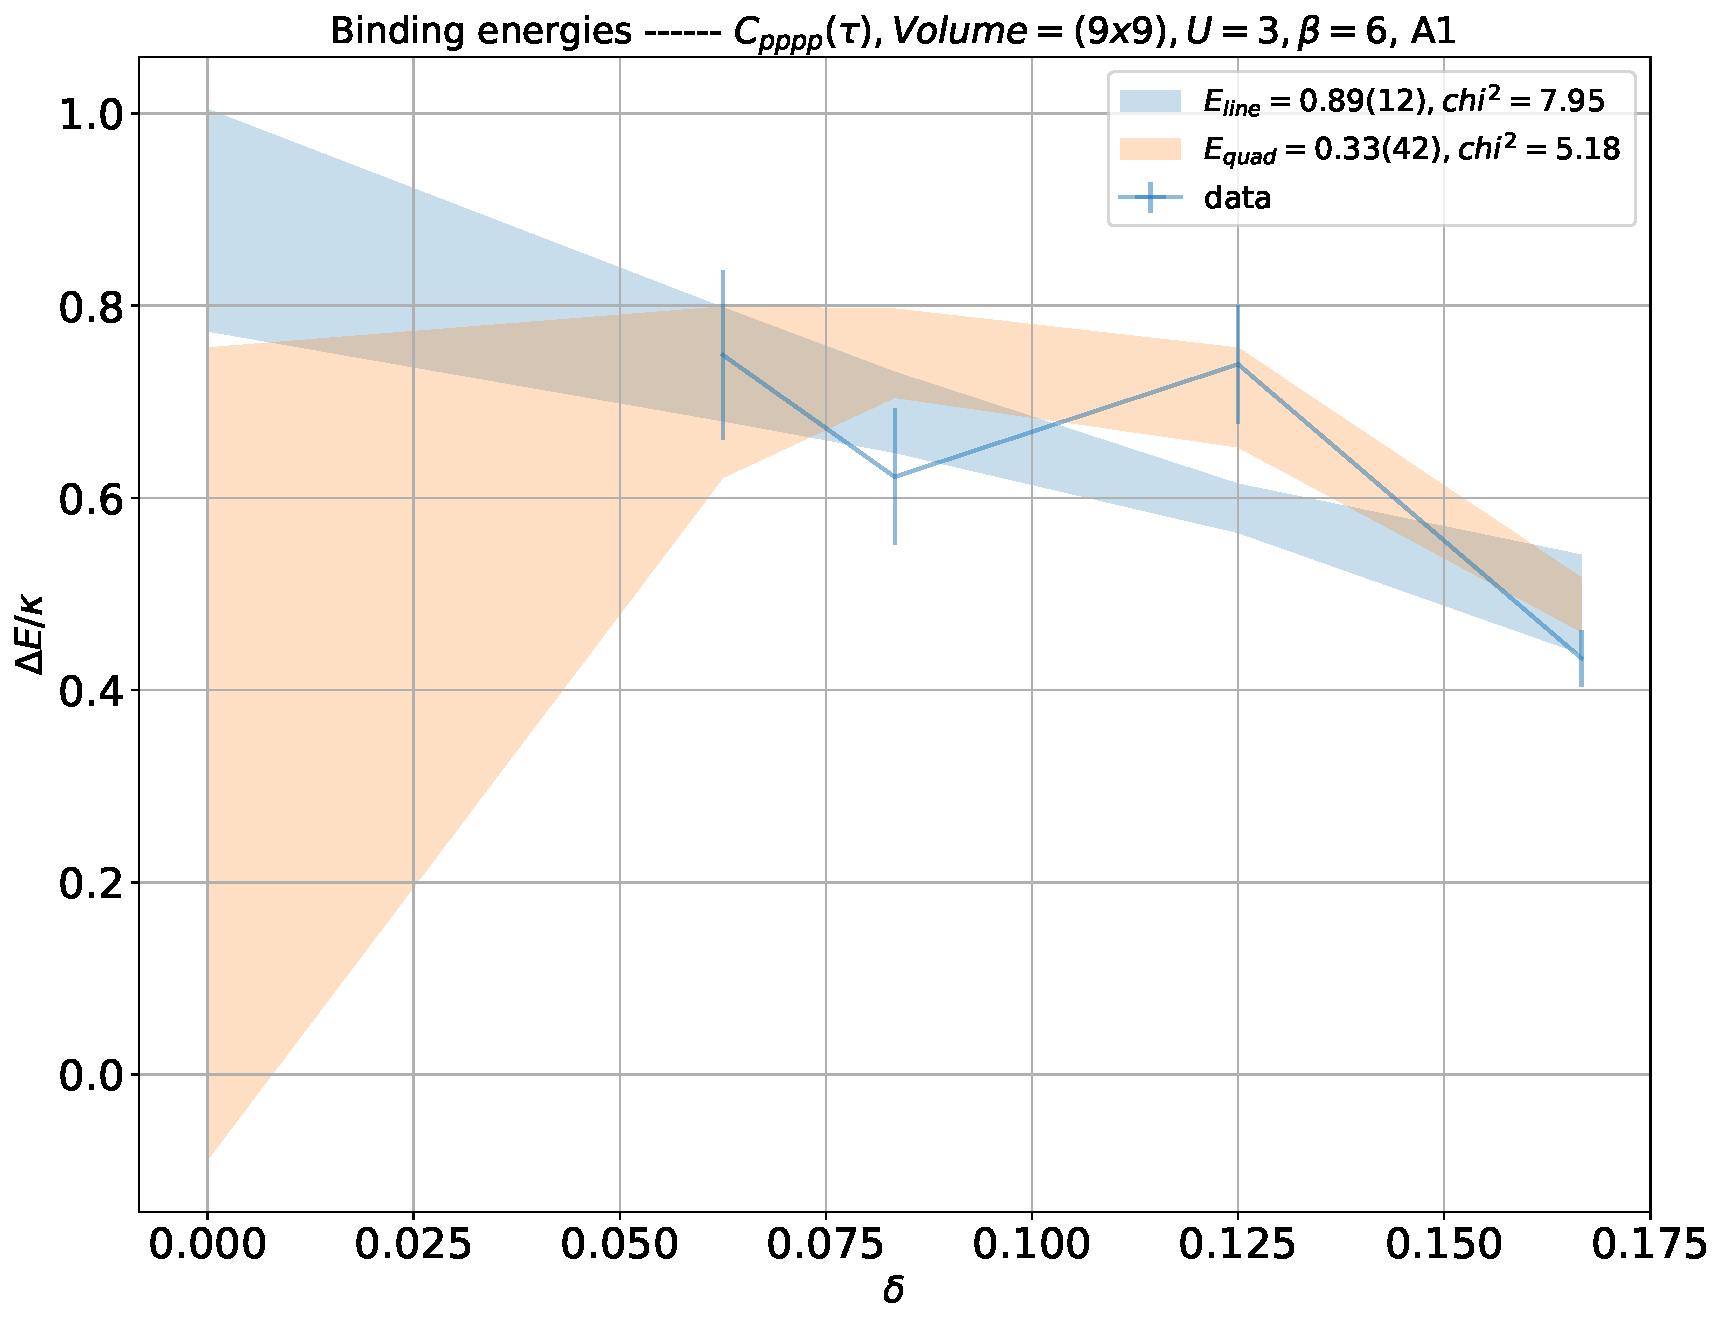
\includegraphics[width=\linewidth]{pppp-0-A1_9x9_U3_B6_cont.pdf}
  \end{subfigure}
  \begin{subfigure}{.5\textwidth}
      \centering
      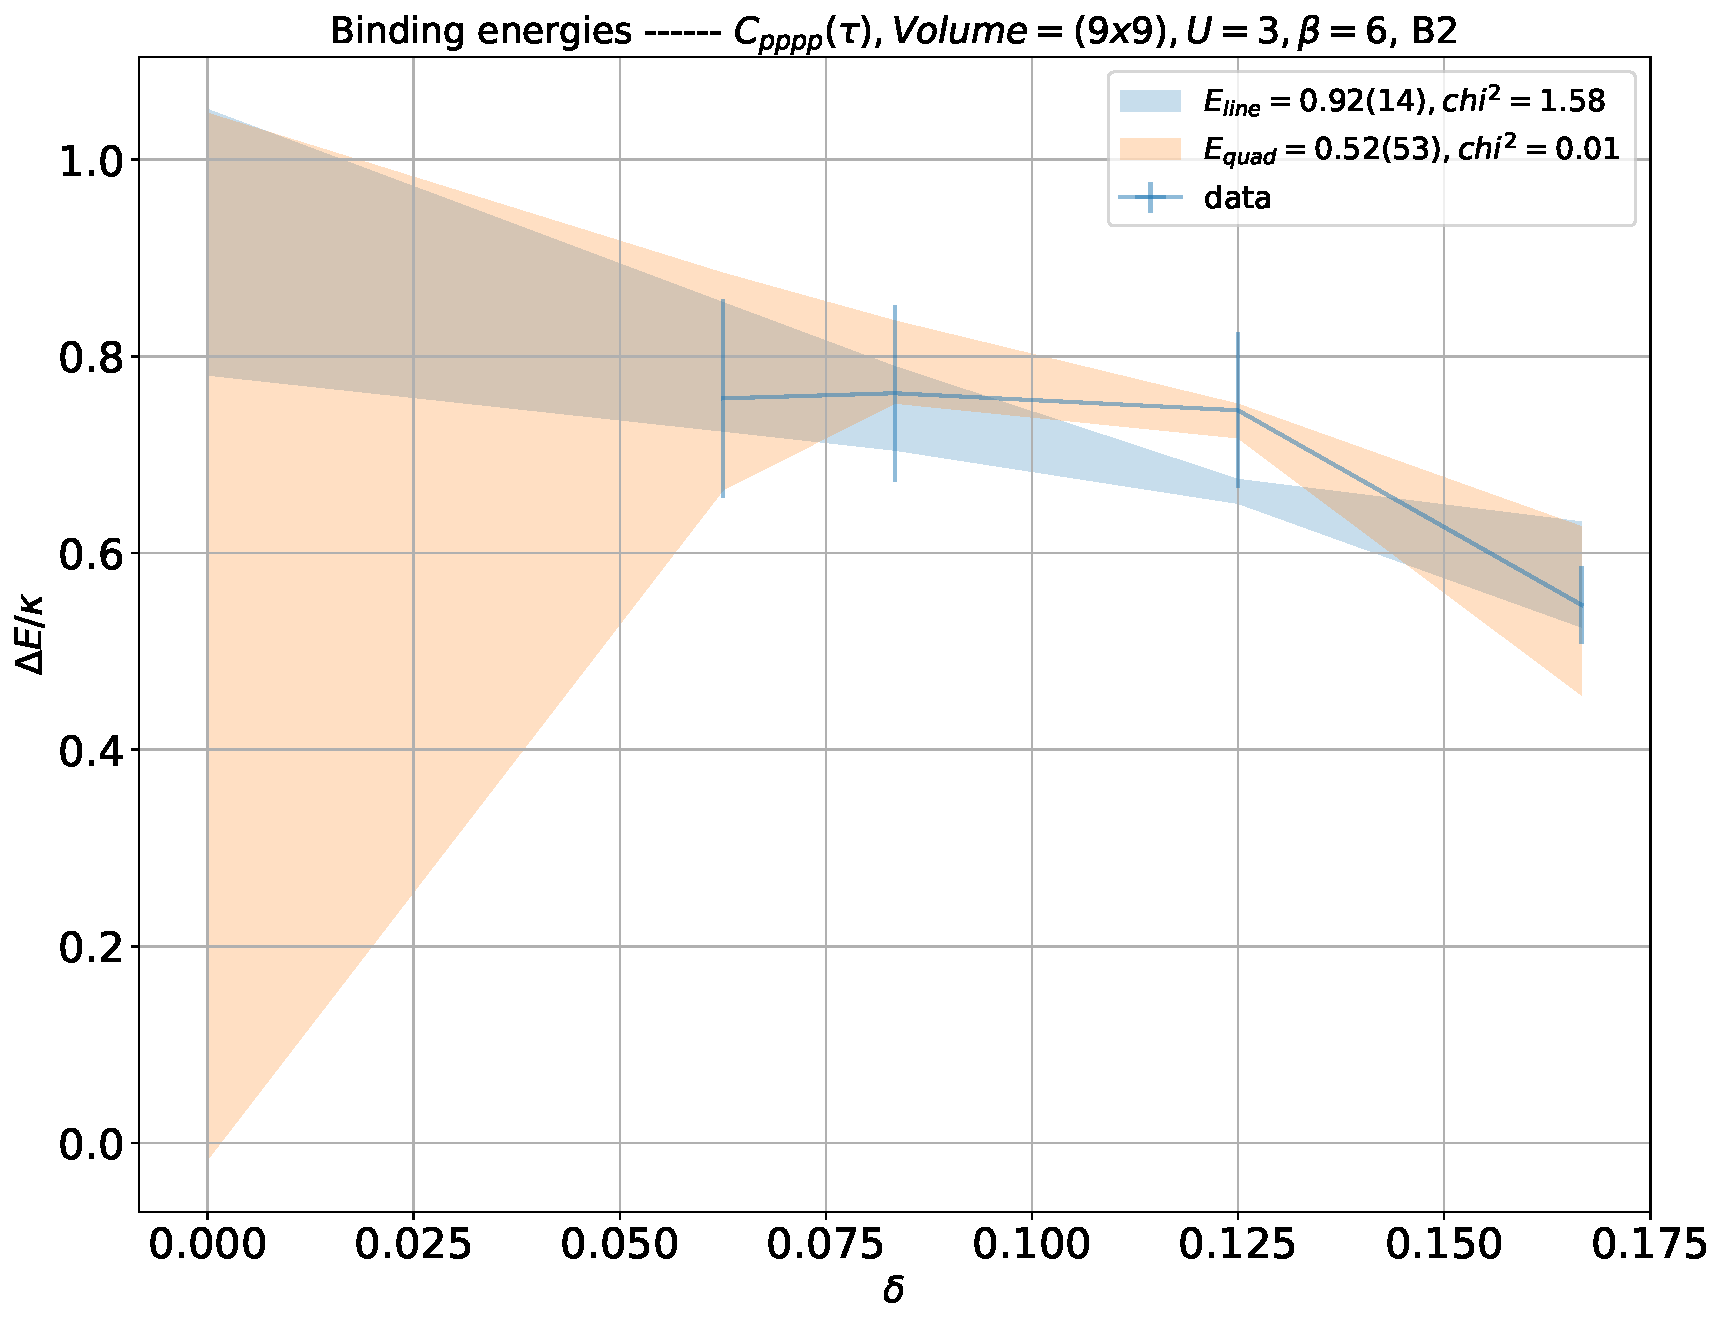
\includegraphics[width=\linewidth]{pppp-0-B2_9x9_U3_B6_cont.pdf}
  \end{subfigure}
  \caption{Binding energy extraction of the particle-particle pair at both irreducible representations, where we fit one- and two-body correlators for every $N_t$. This is followed by fitting a linear and a quadratic functions to the $\Delta E_{N_t}$ in order to extrapolate to the continuum limit ($N_t\to\infty$).}
  \label{fig:fig7}
\end{figure}

\begin{figure}
  \begin{subfigure}{.5\textwidth}
    \centering
    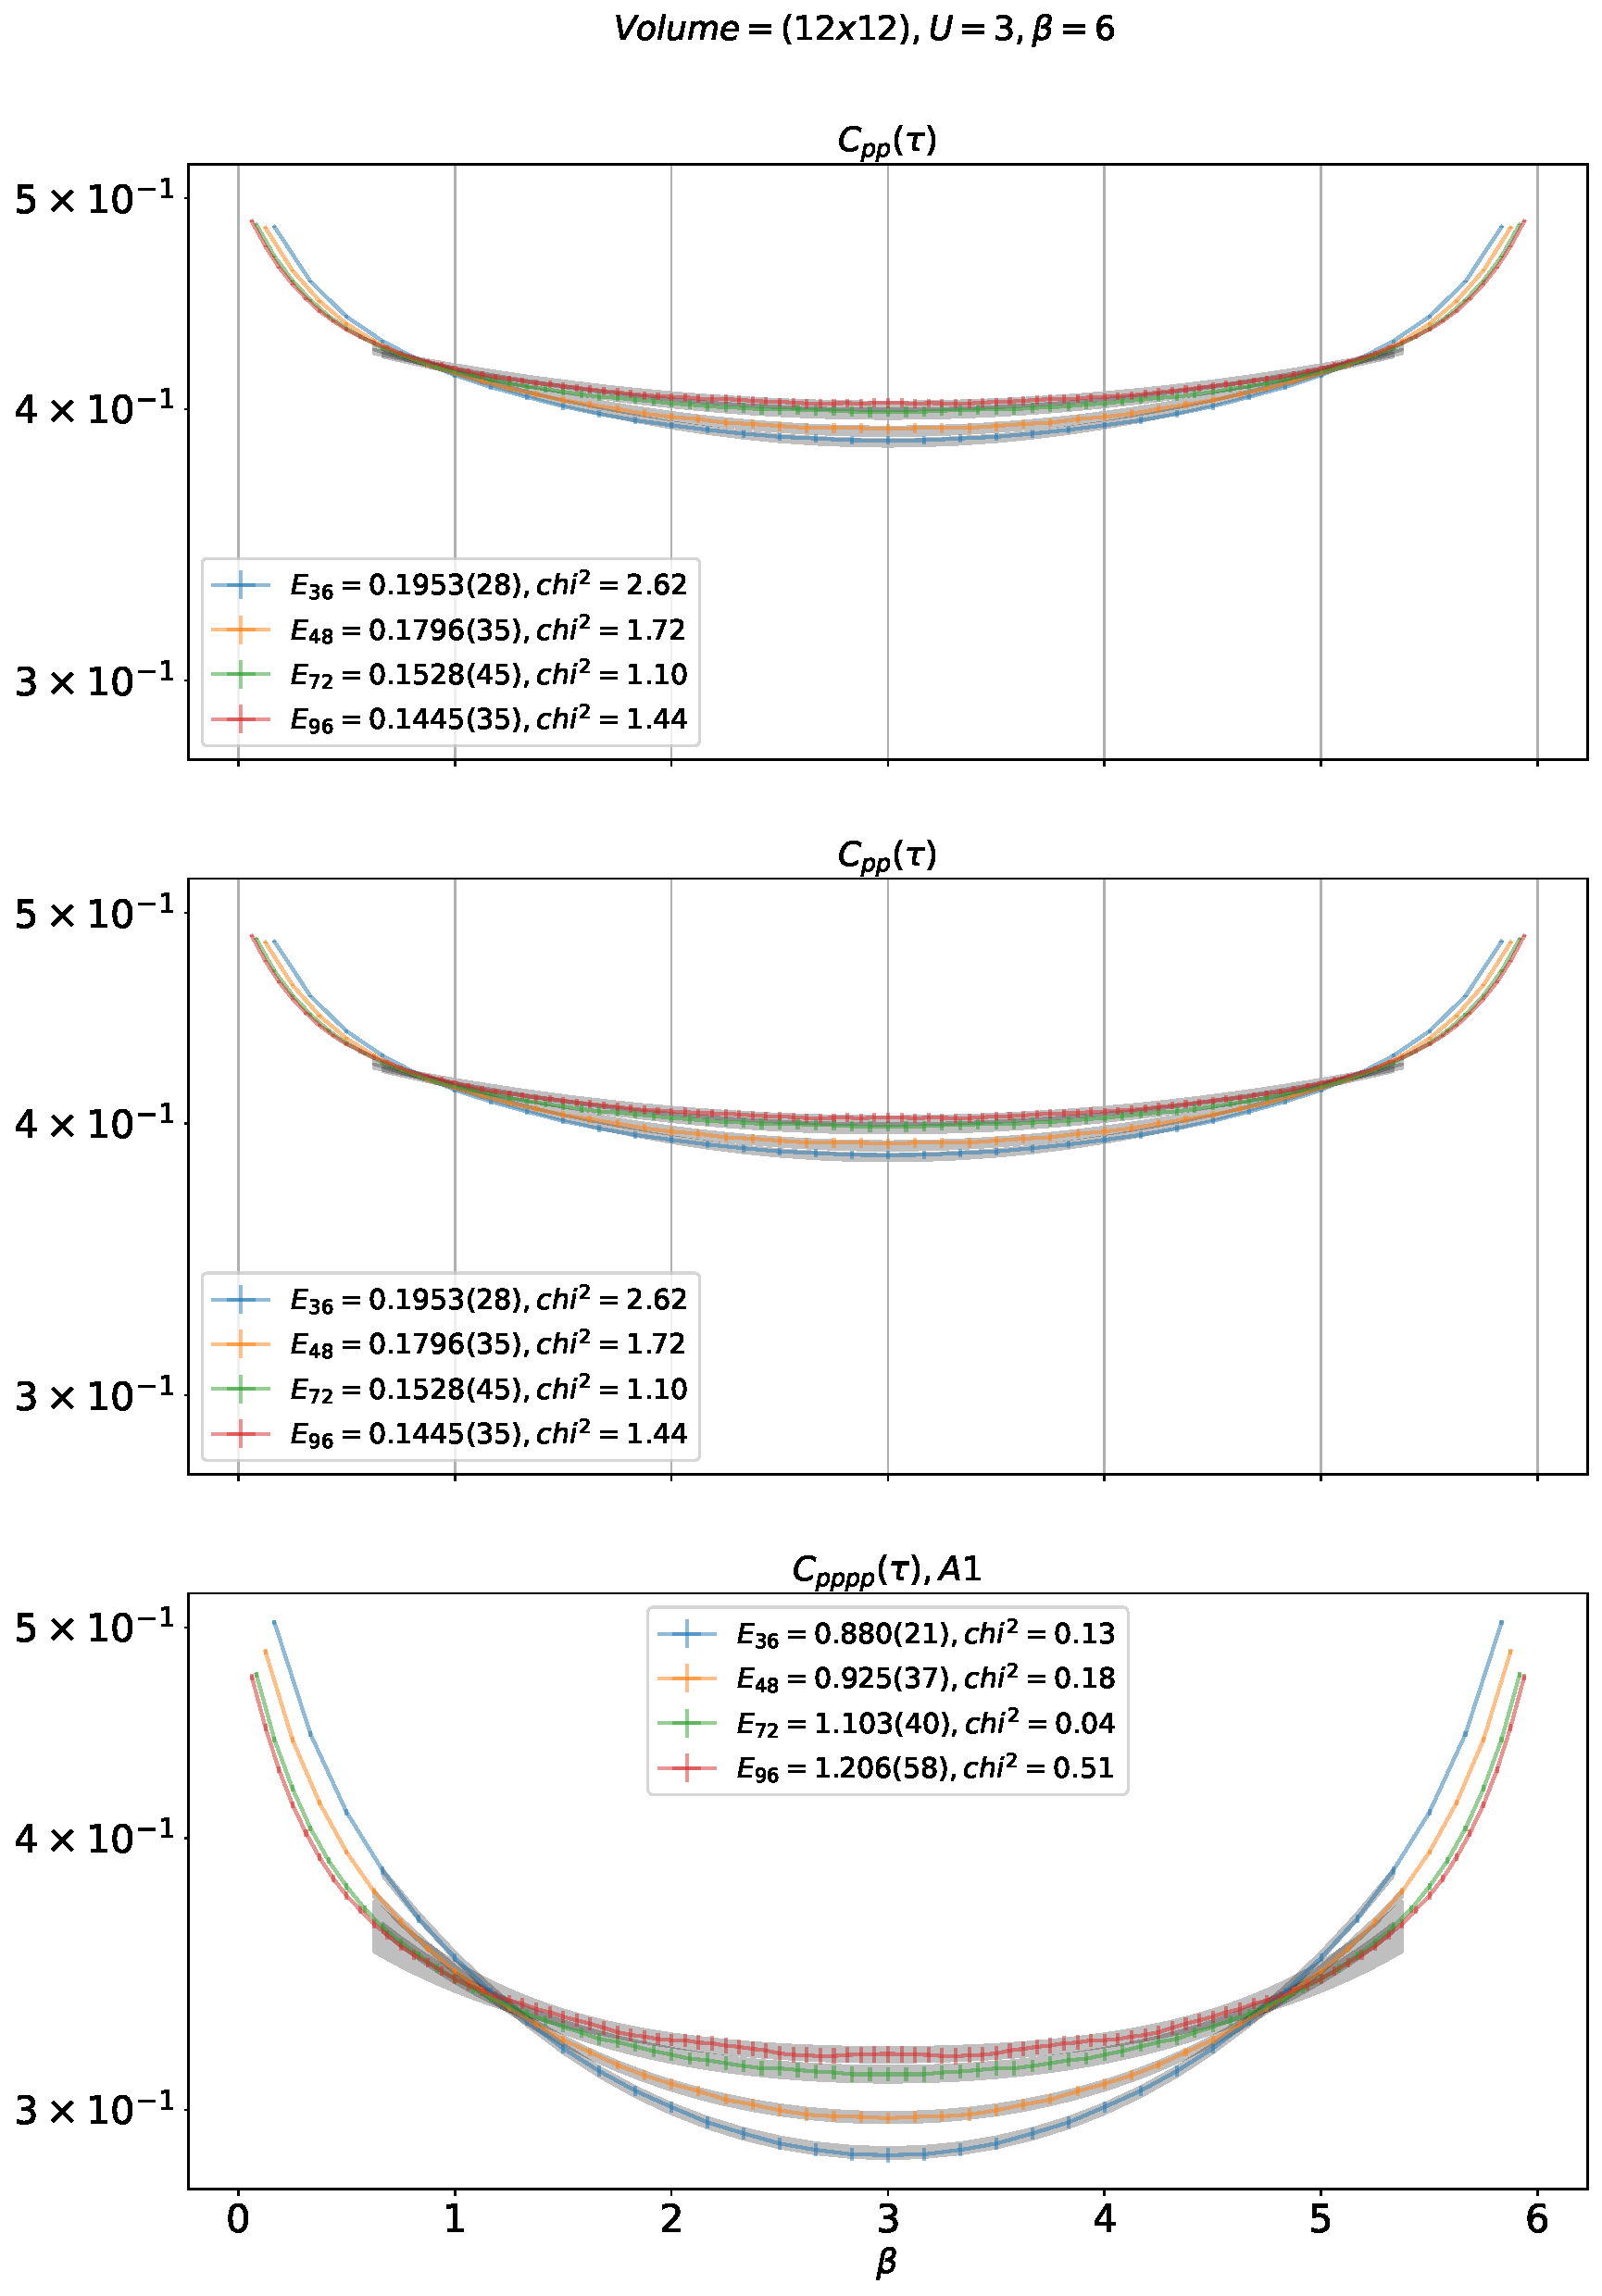
\includegraphics[width=\linewidth]{pppp-0-A1_12x12_U3_B6.pdf}
  \end{subfigure}%
  \begin{subfigure}{.5\textwidth}
    \centering
    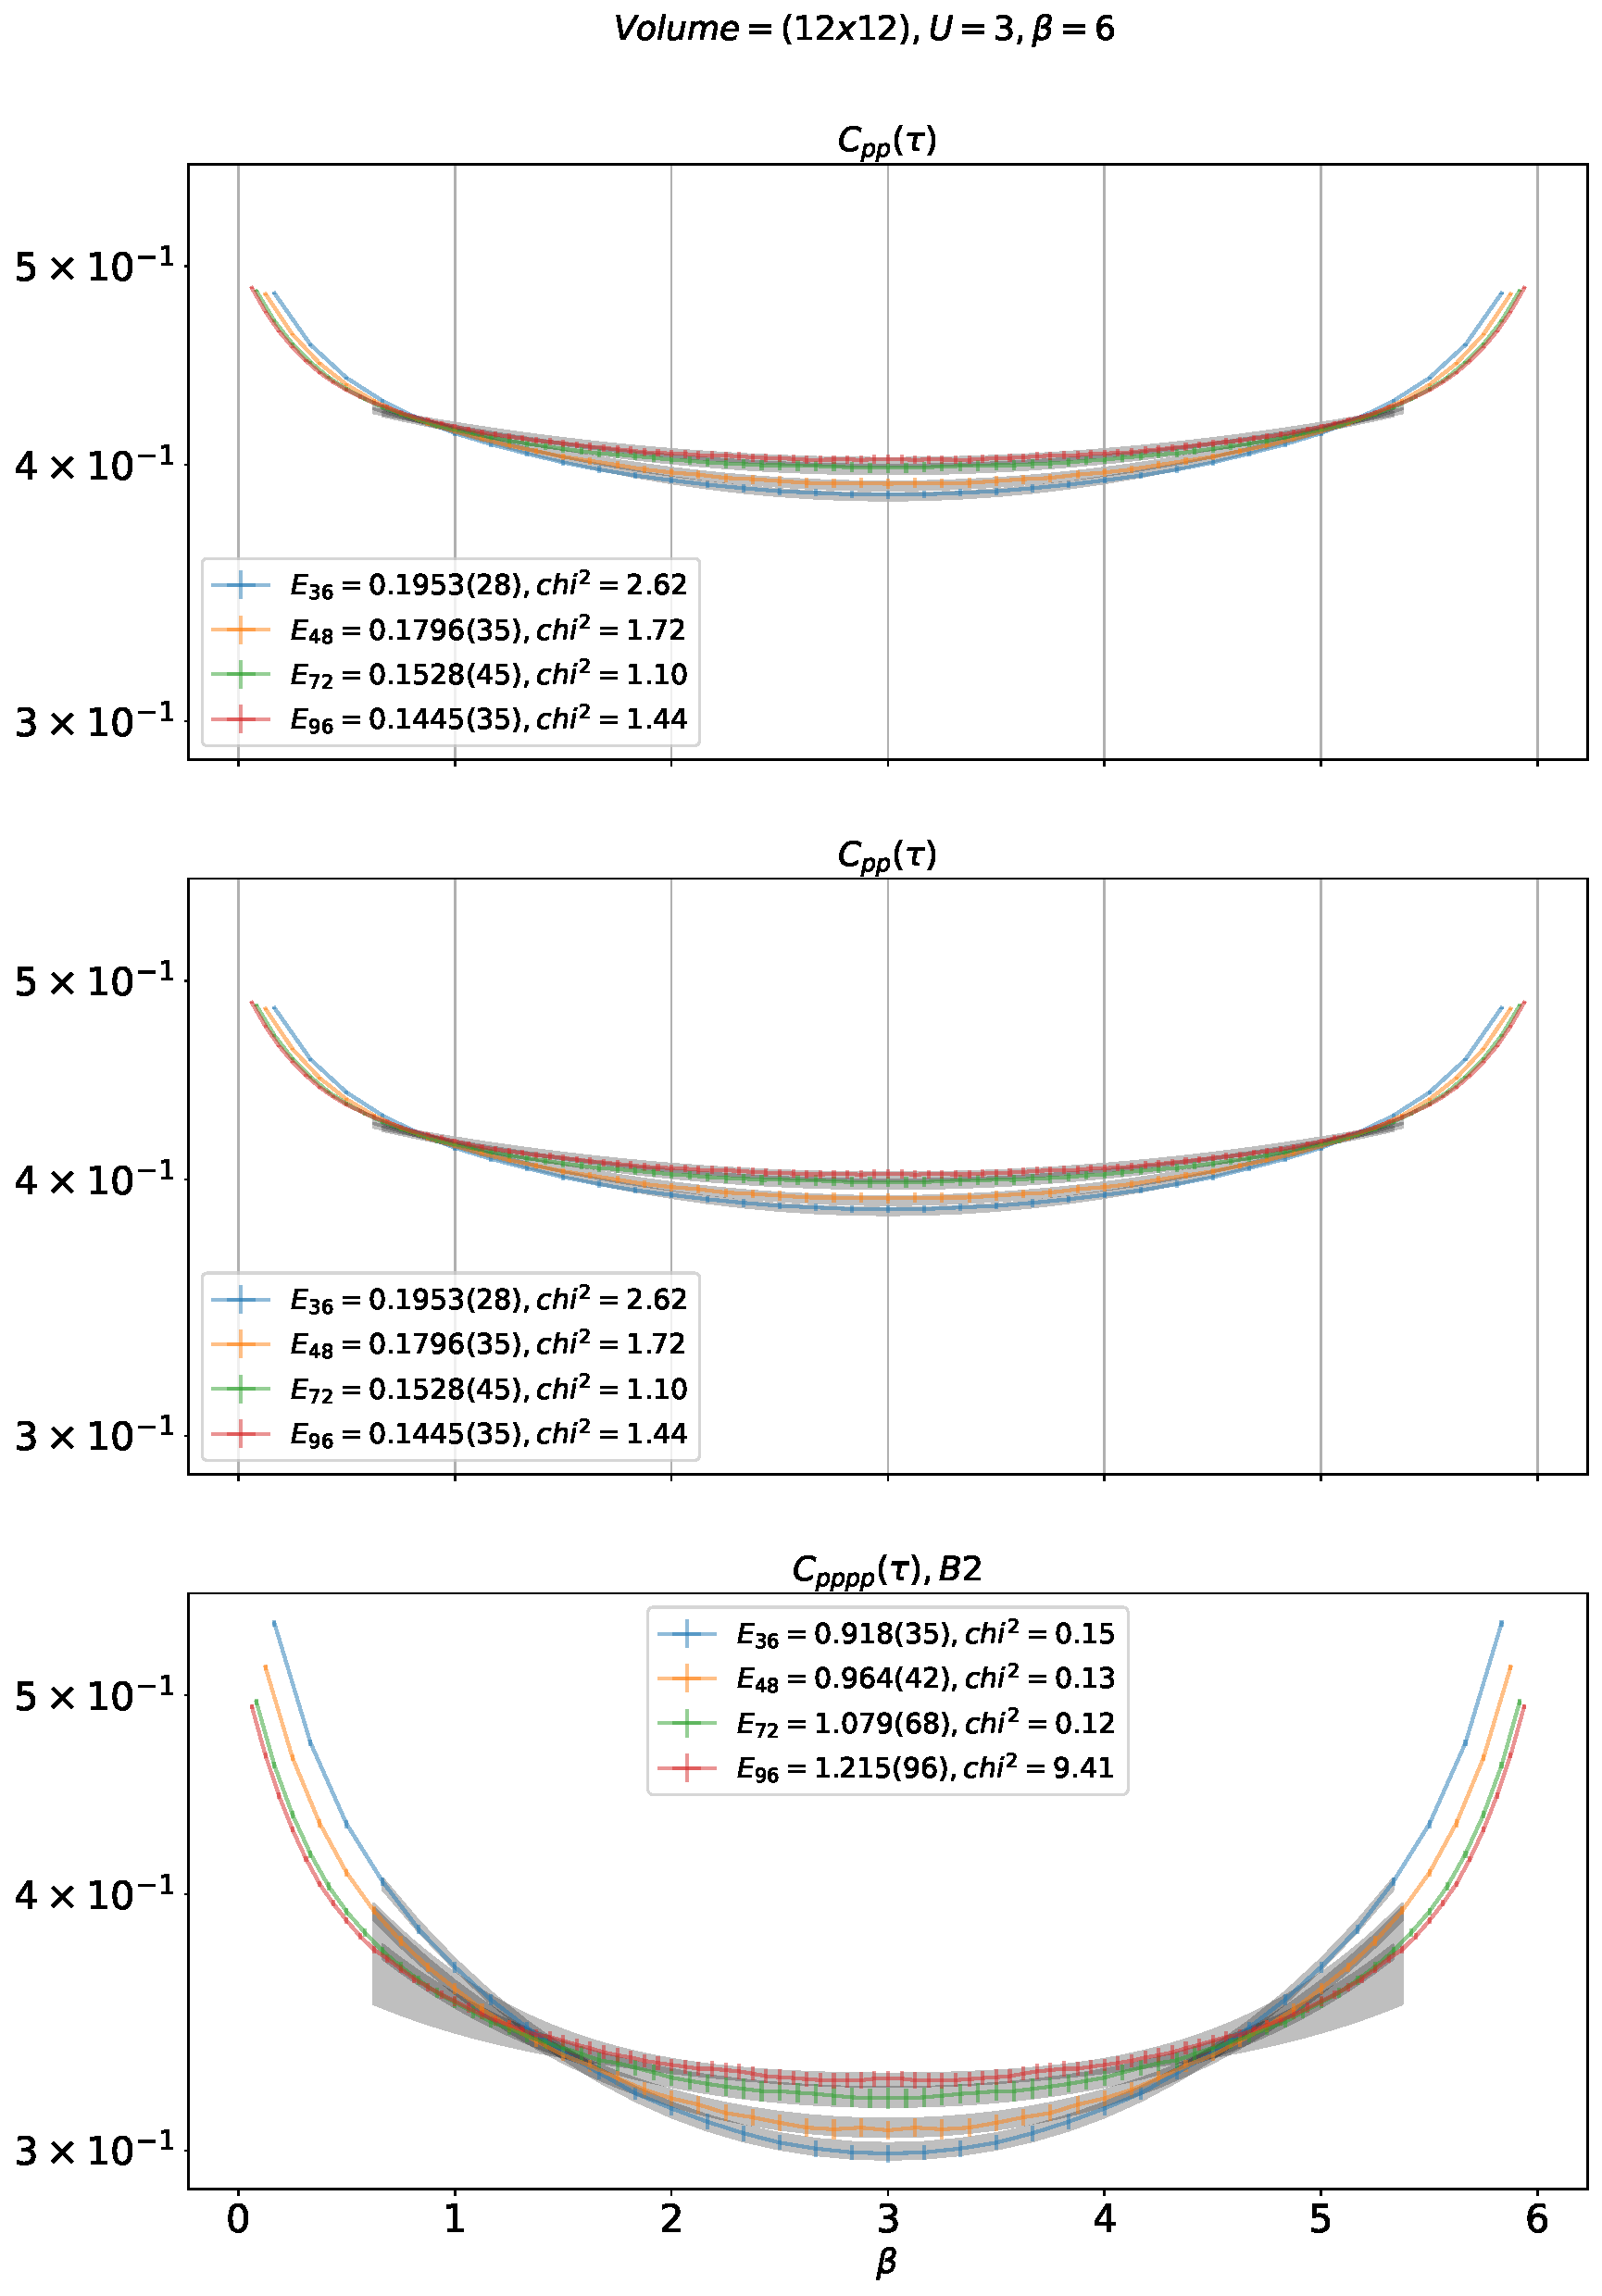
\includegraphics[width=\linewidth]{pppp-0-B2_12x12_U3_B6.pdf}
  \end{subfigure}
  \begin{subfigure}{.5\textwidth}
      \centering
      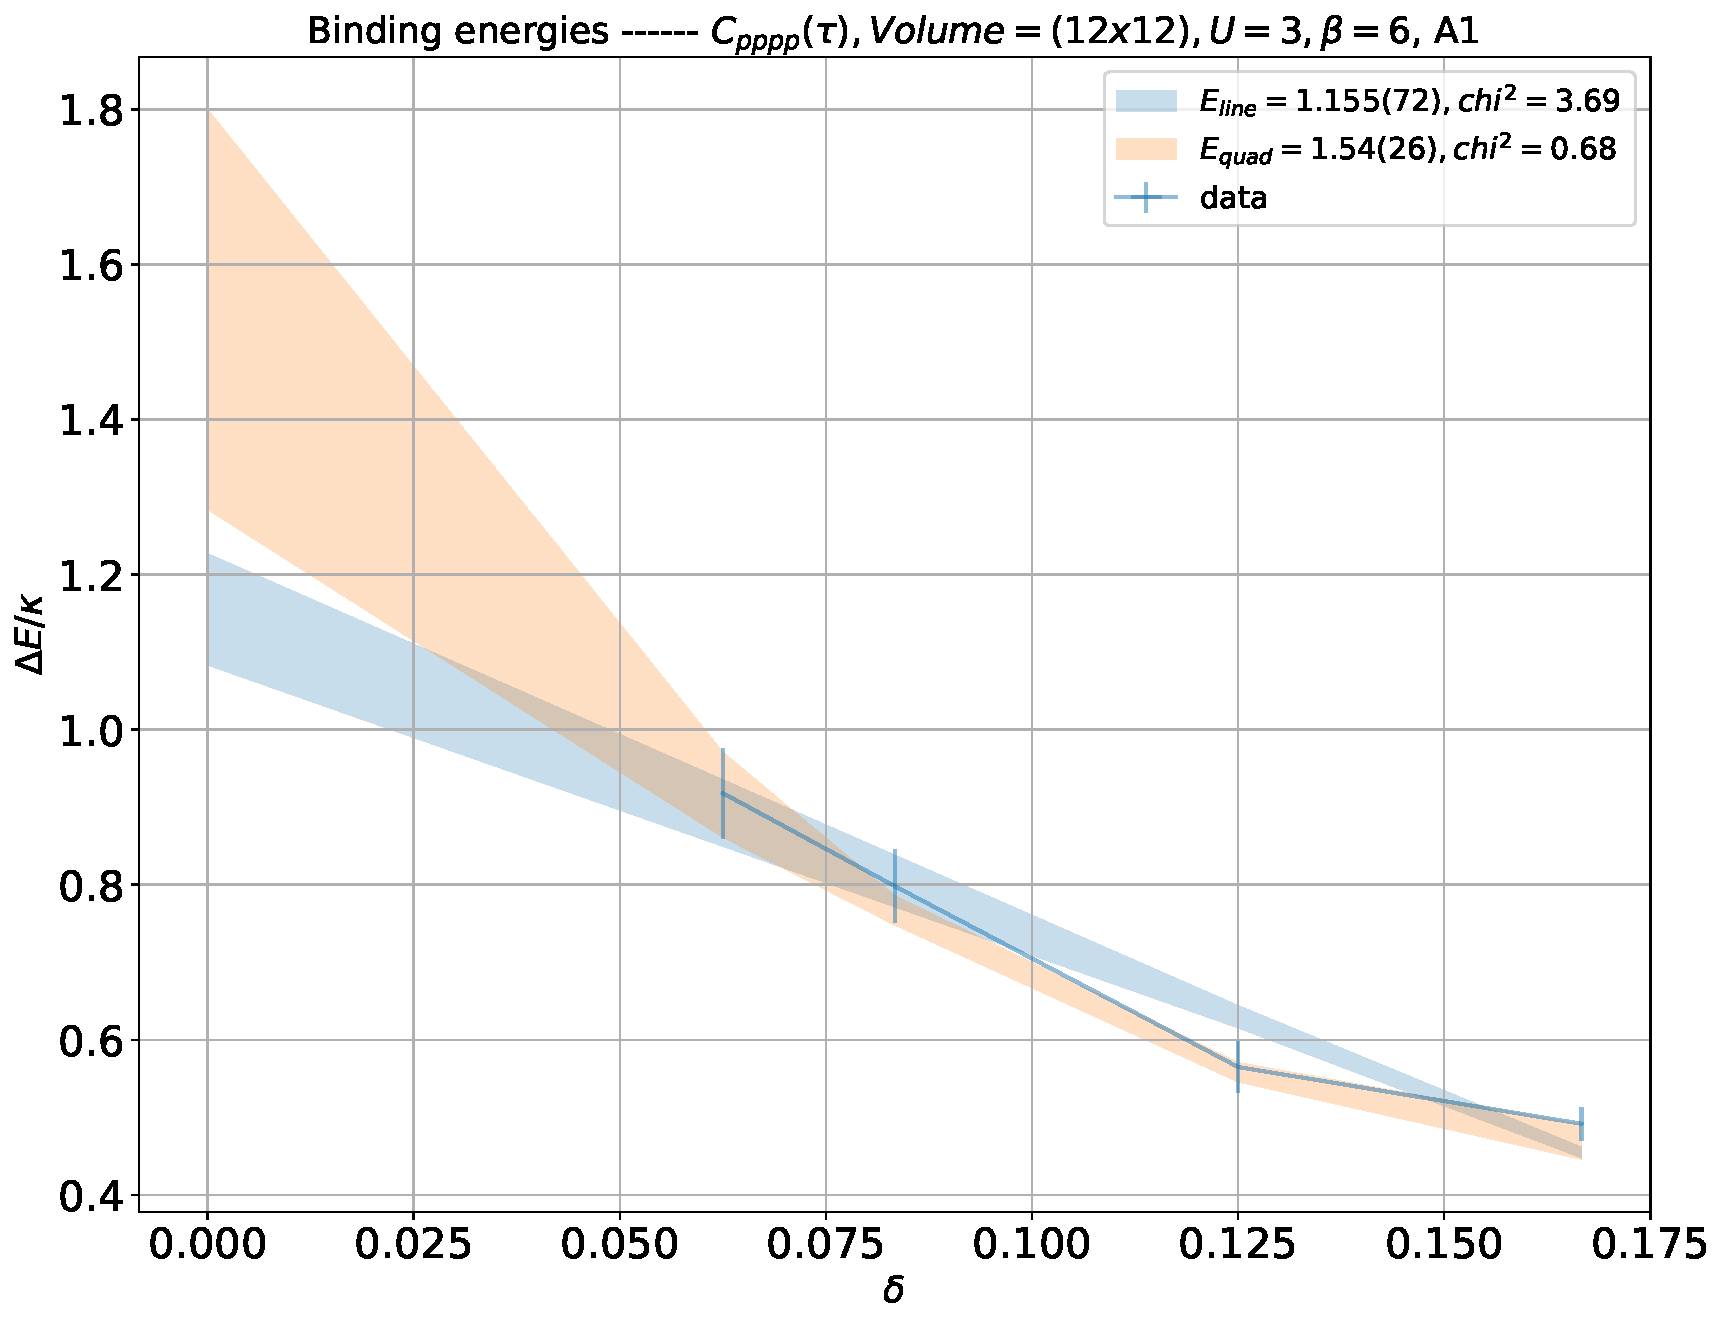
\includegraphics[width=\linewidth]{pppp-0-A1_12x12_U3_B6_cont.pdf}
  \end{subfigure}
  \begin{subfigure}{.5\textwidth}
      \centering
      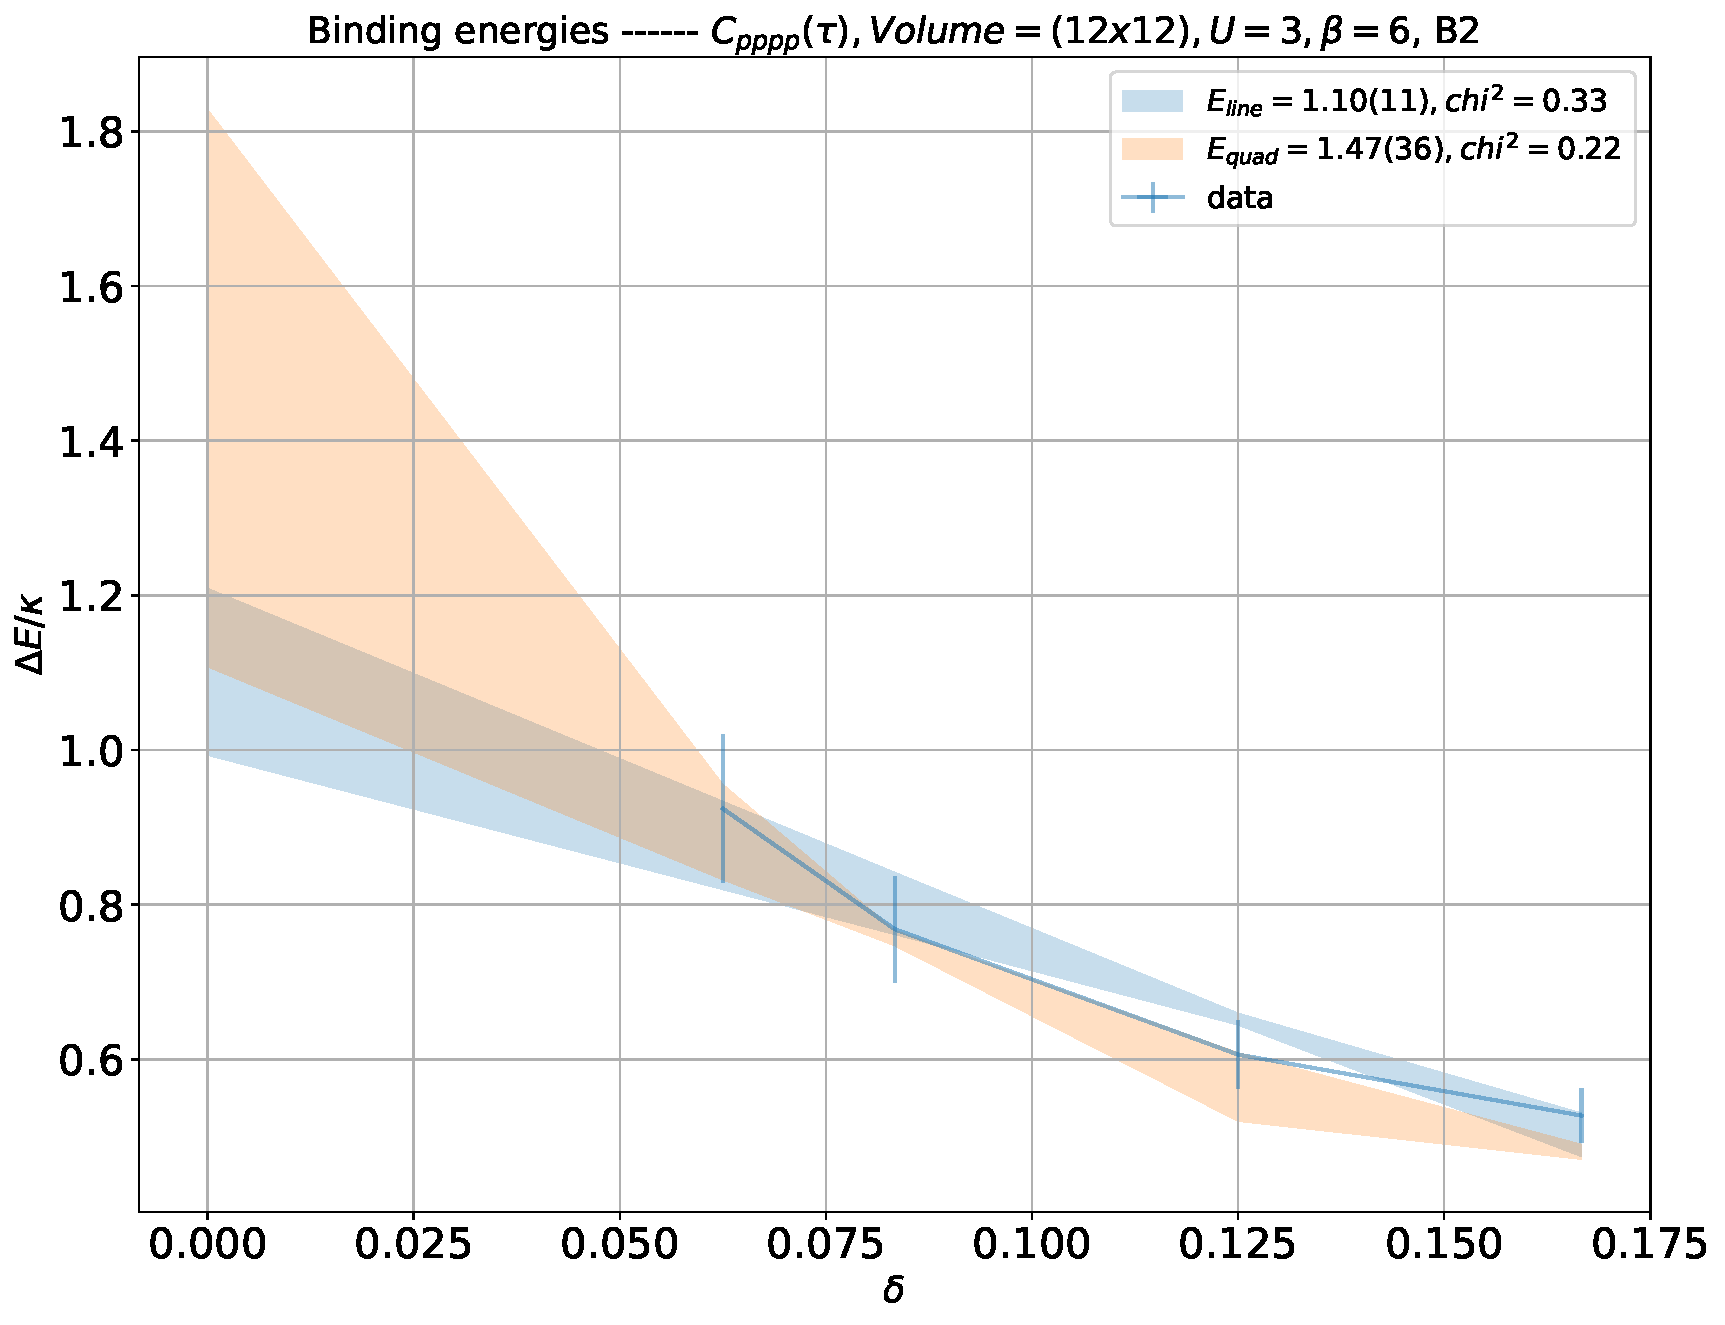
\includegraphics[width=\linewidth]{pppp-0-B2_12x12_U3_B6_cont.pdf}
  \end{subfigure}
  \caption{Binding energy extraction of the particle-particle pair at both irreducible representations, where we fit one- and two-body correlators for every $N_t$. This is followed by fitting a linear and a quadratic functions to the $\Delta E_{N_t}$ in order to extrapolate to the continuum limit ($N_t\to\infty$).}
  \label{fig:fig8}
\end{figure}

\begin{figure}
  \begin{subfigure}{.5\textwidth}
    \centering
    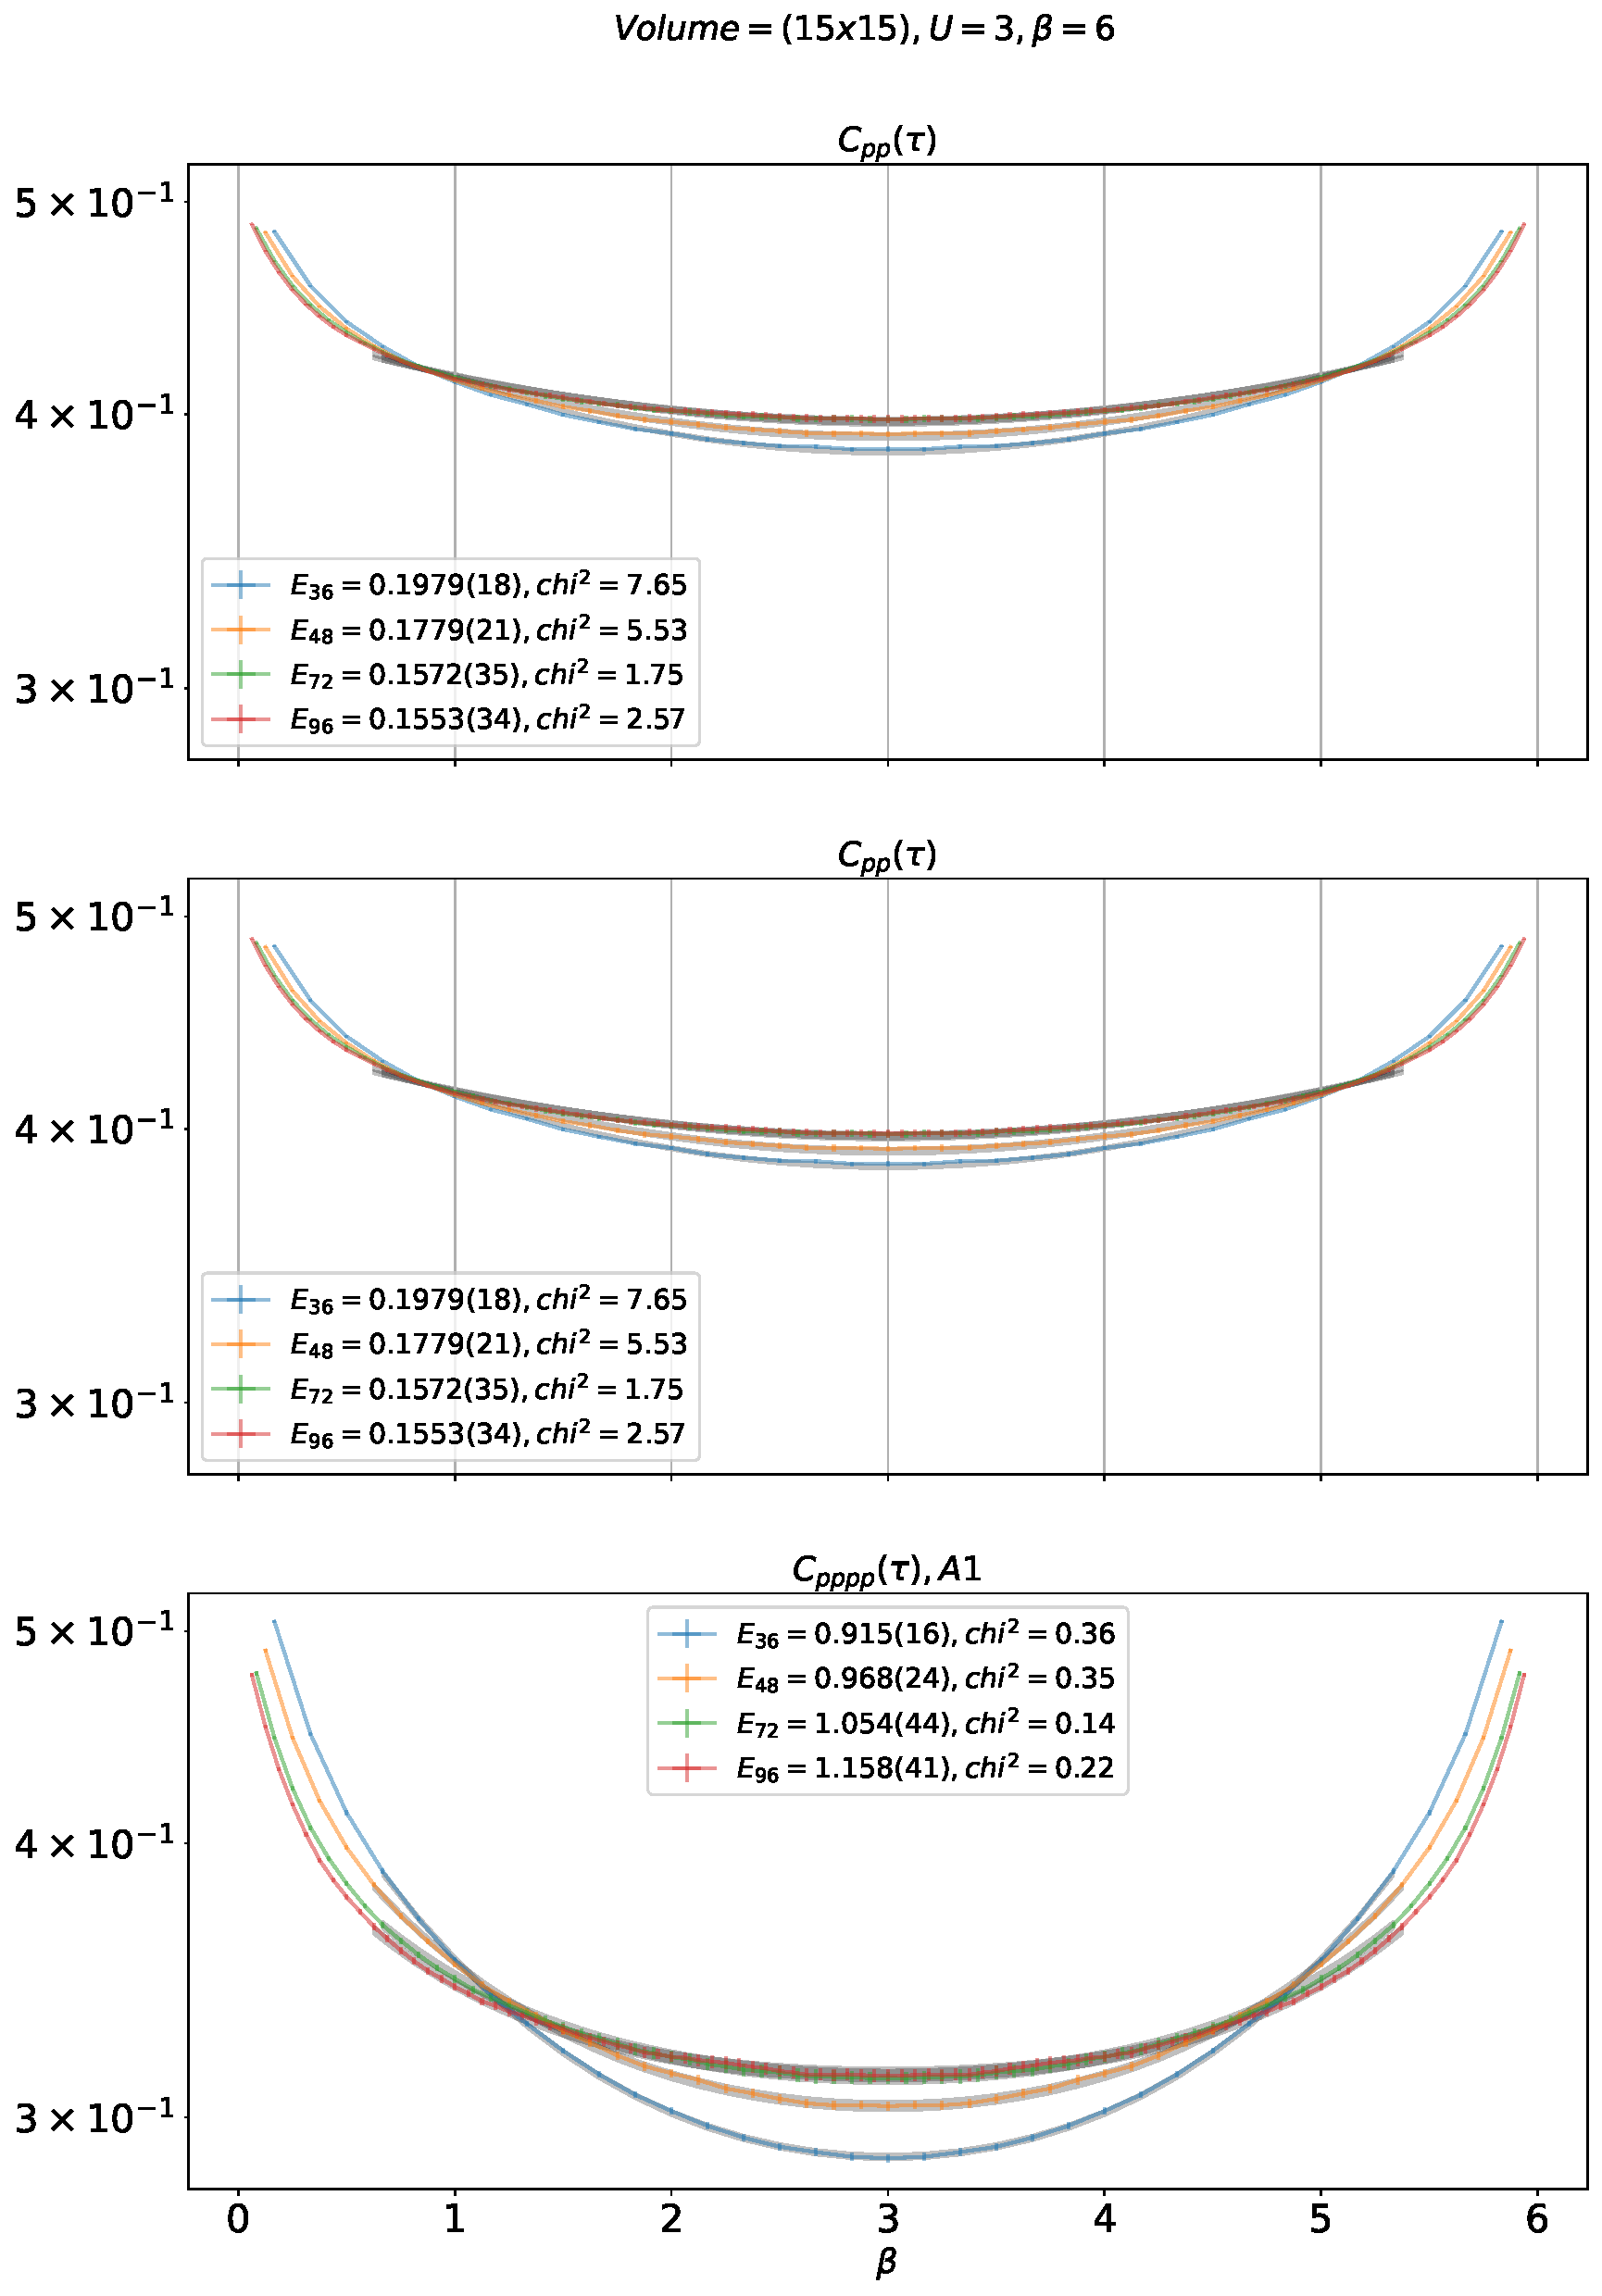
\includegraphics[width=\linewidth]{pppp-0-A1_15x15_U3_B6.pdf}
  \end{subfigure}%
  \begin{subfigure}{.5\textwidth}
    \centering
    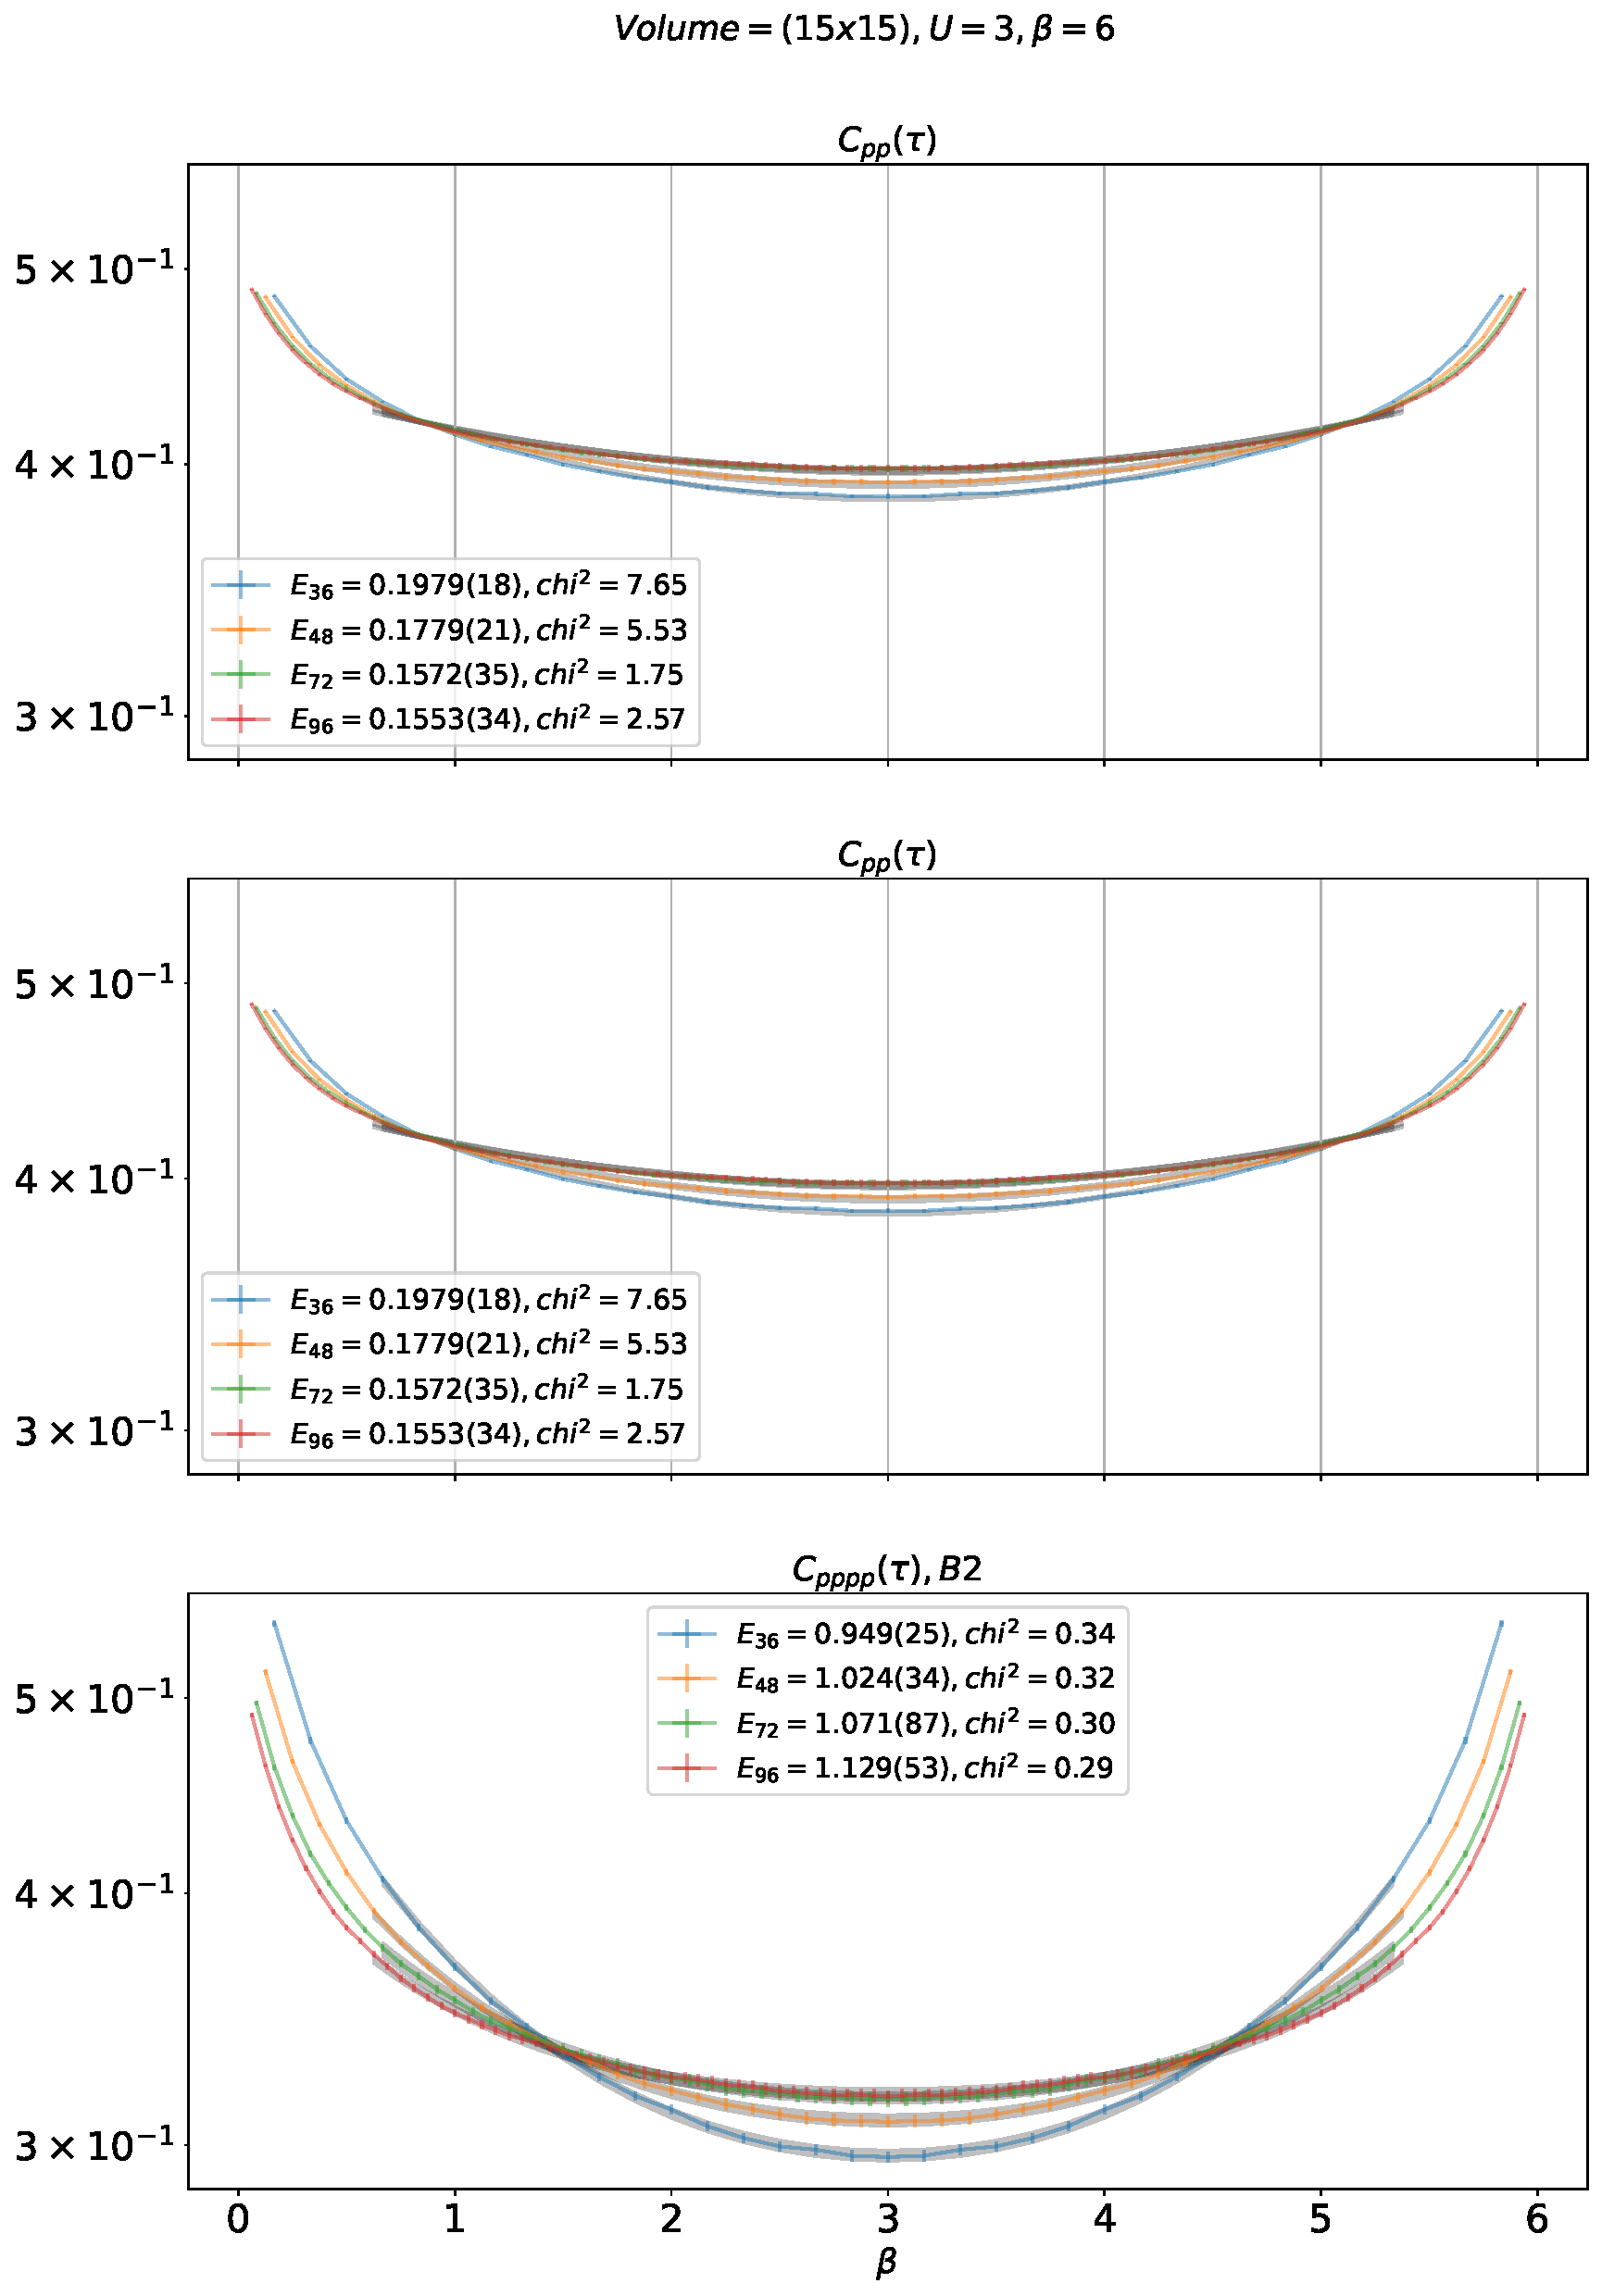
\includegraphics[width=\linewidth]{pppp-0-B2_15x15_U3_B6.pdf}
  \end{subfigure}
  \begin{subfigure}{.5\textwidth}
      \centering
      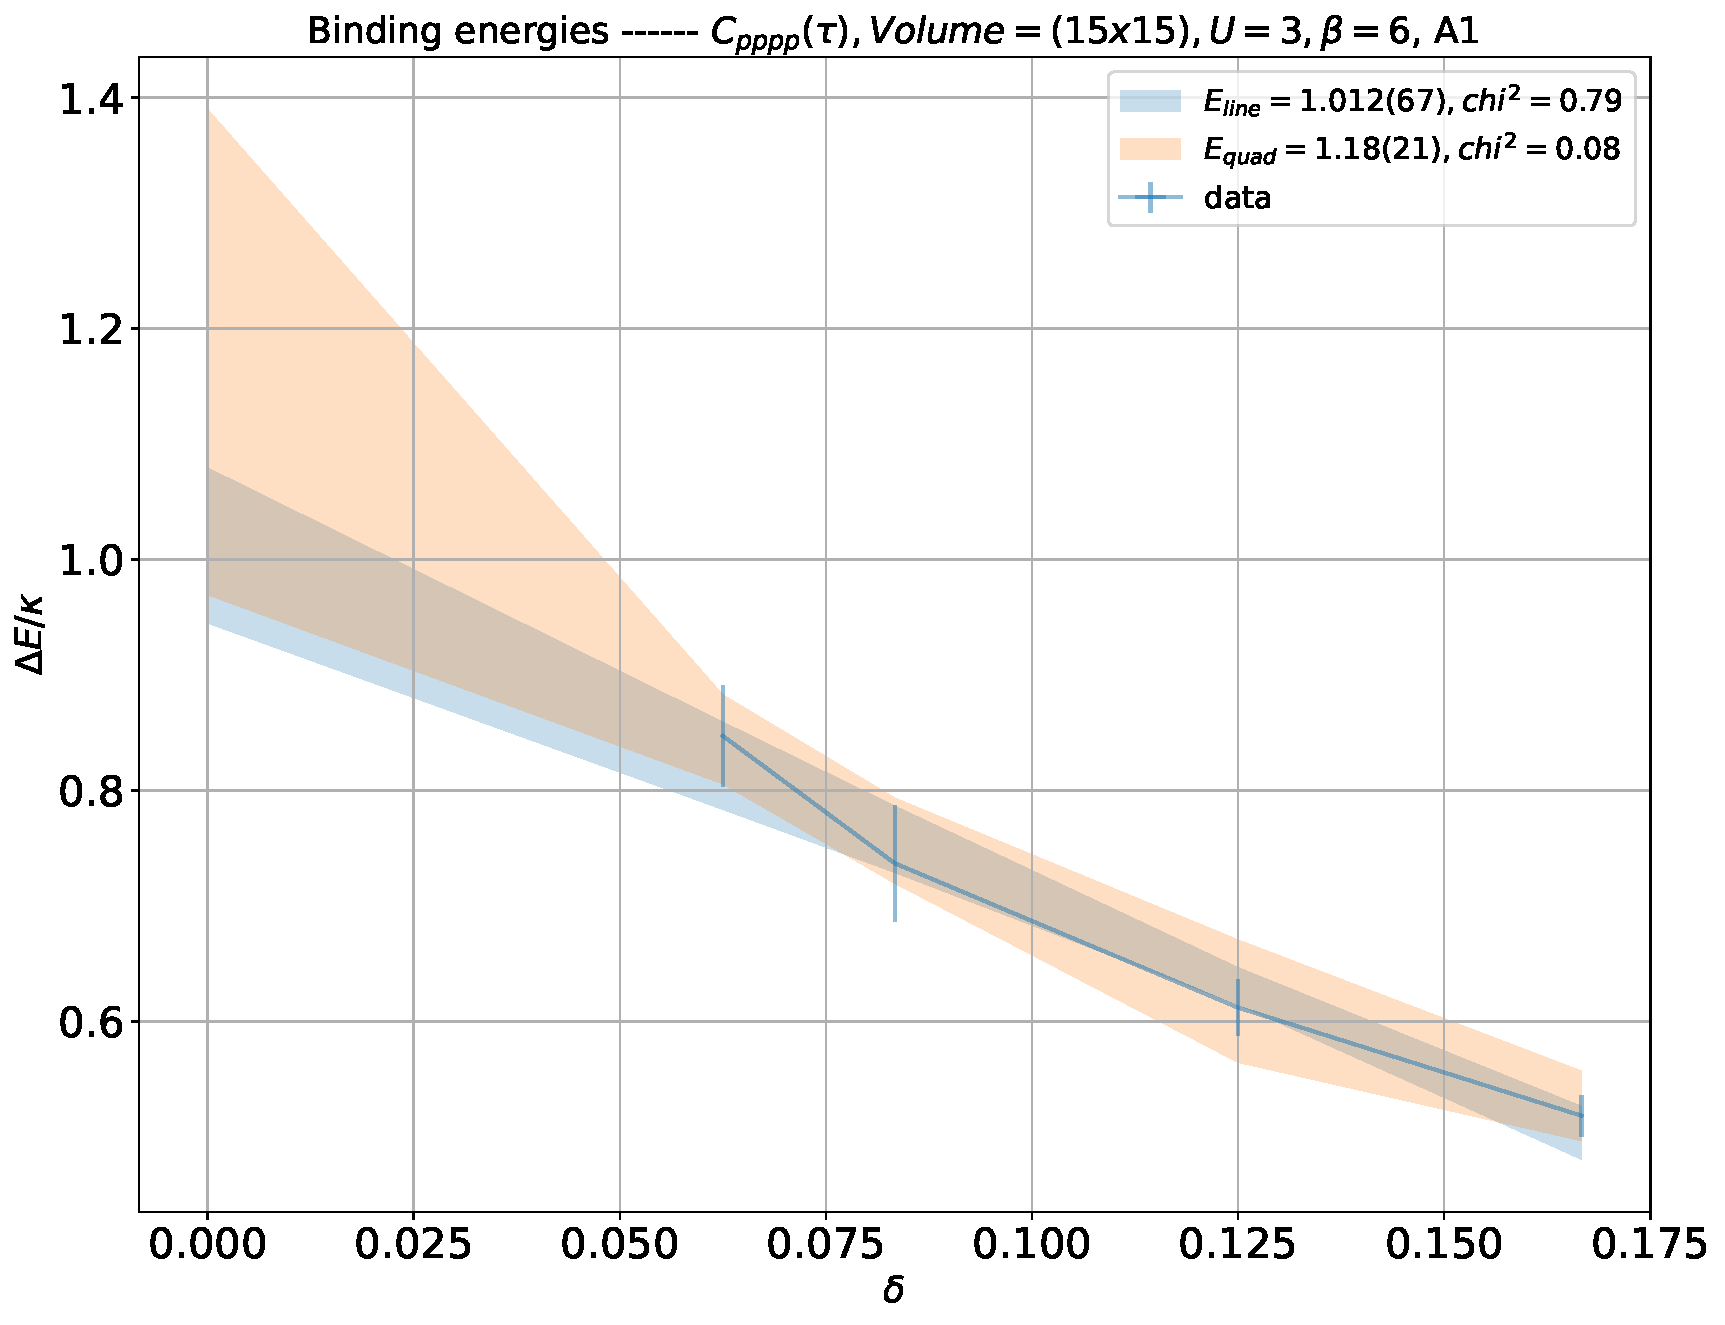
\includegraphics[width=\linewidth]{pppp-0-A1_15x15_U3_B6_cont.pdf}
  \end{subfigure}
  \begin{subfigure}{.5\textwidth}
      \centering
      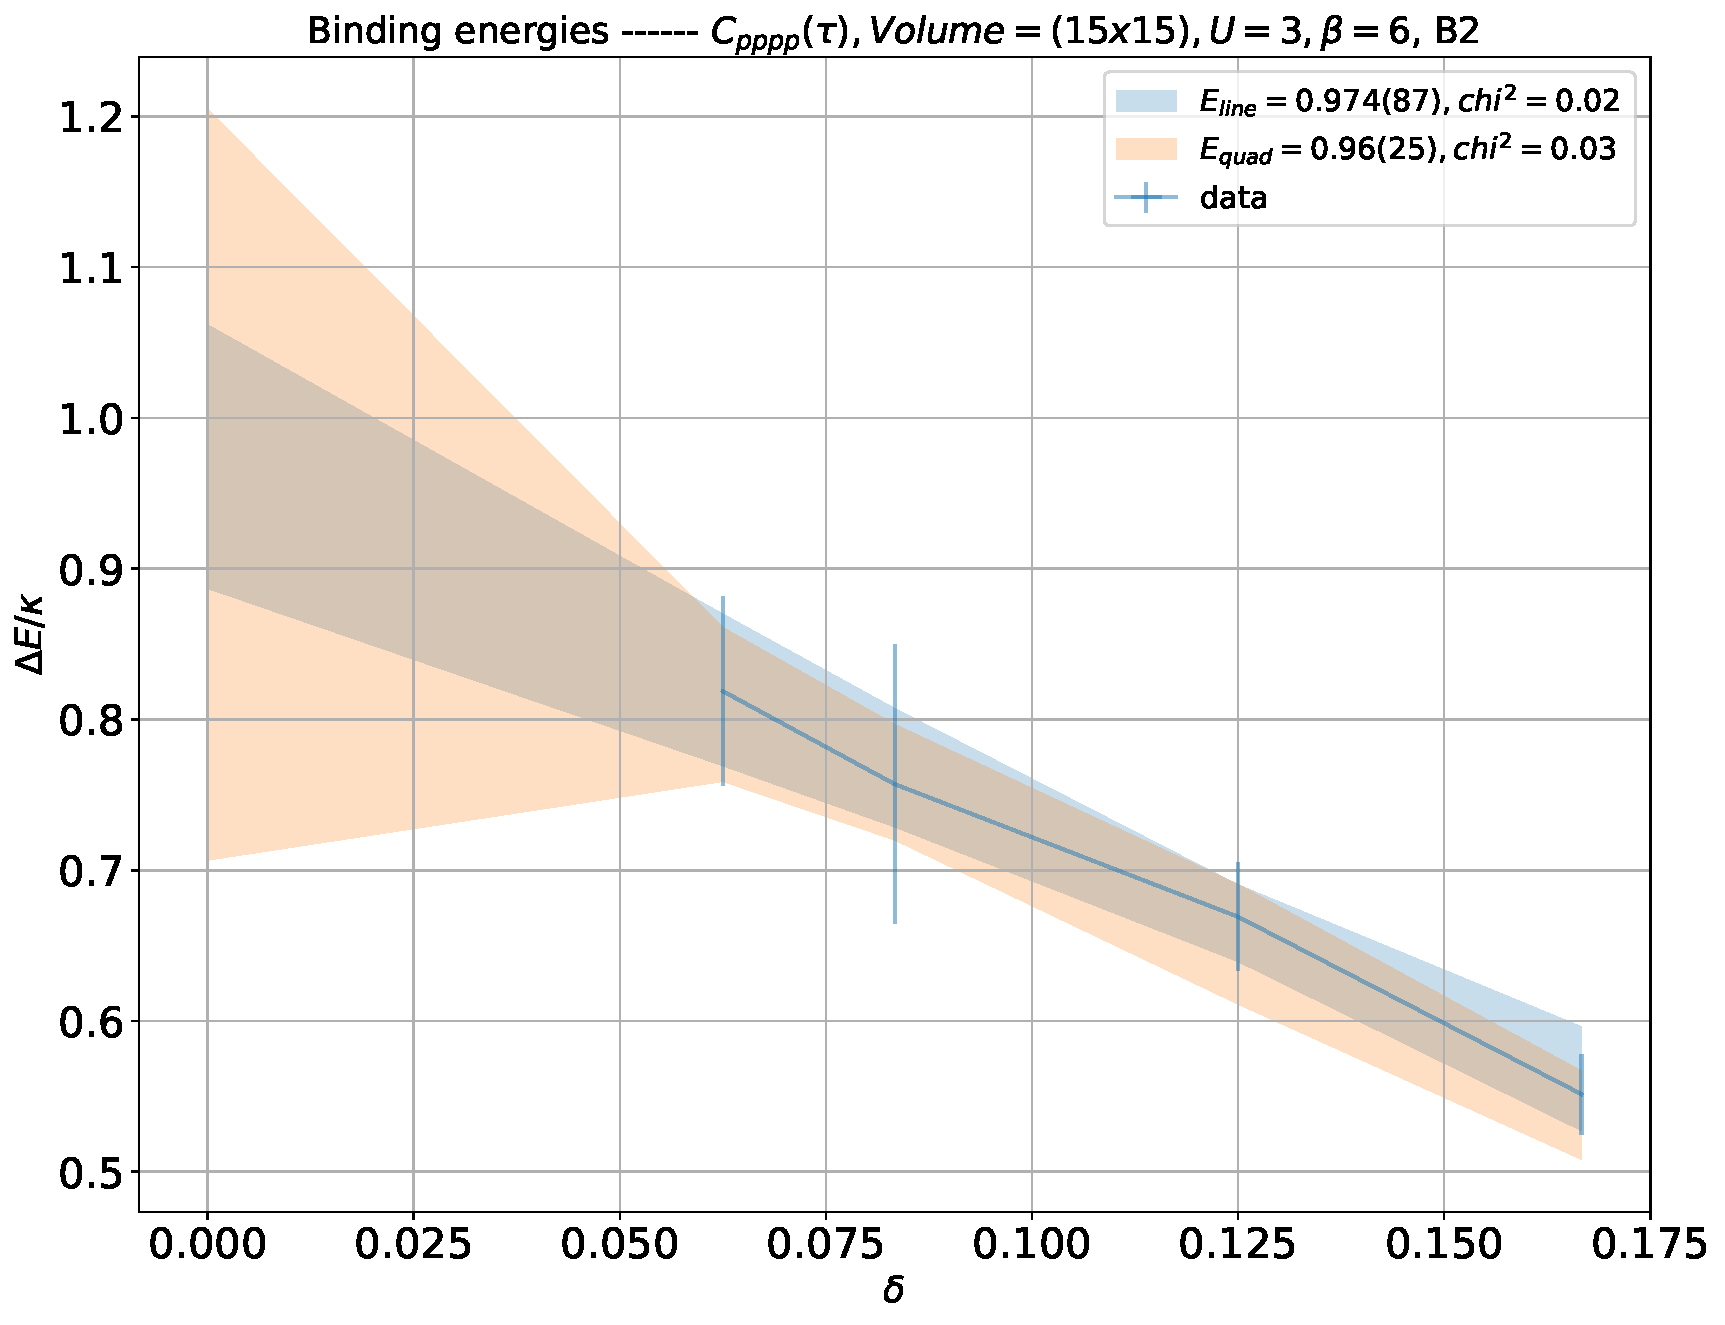
\includegraphics[width=\linewidth]{pppp-0-B2_15x15_U3_B6_cont.pdf}
  \end{subfigure}
  \caption{Binding energy extraction of the particle-particle pair at both irreducible representations, where we fit one- and two-body correlators for every $N_t$. This is followed by fitting a linear and a quadratic functions to the $\Delta E_{N_t}$ in order to extrapolate to the continuum limit ($N_t\to\infty$).}
  \label{fig:fig9}
\end{figure}

\begin{figure}
  \begin{subfigure}{.5\textwidth}
    \centering
    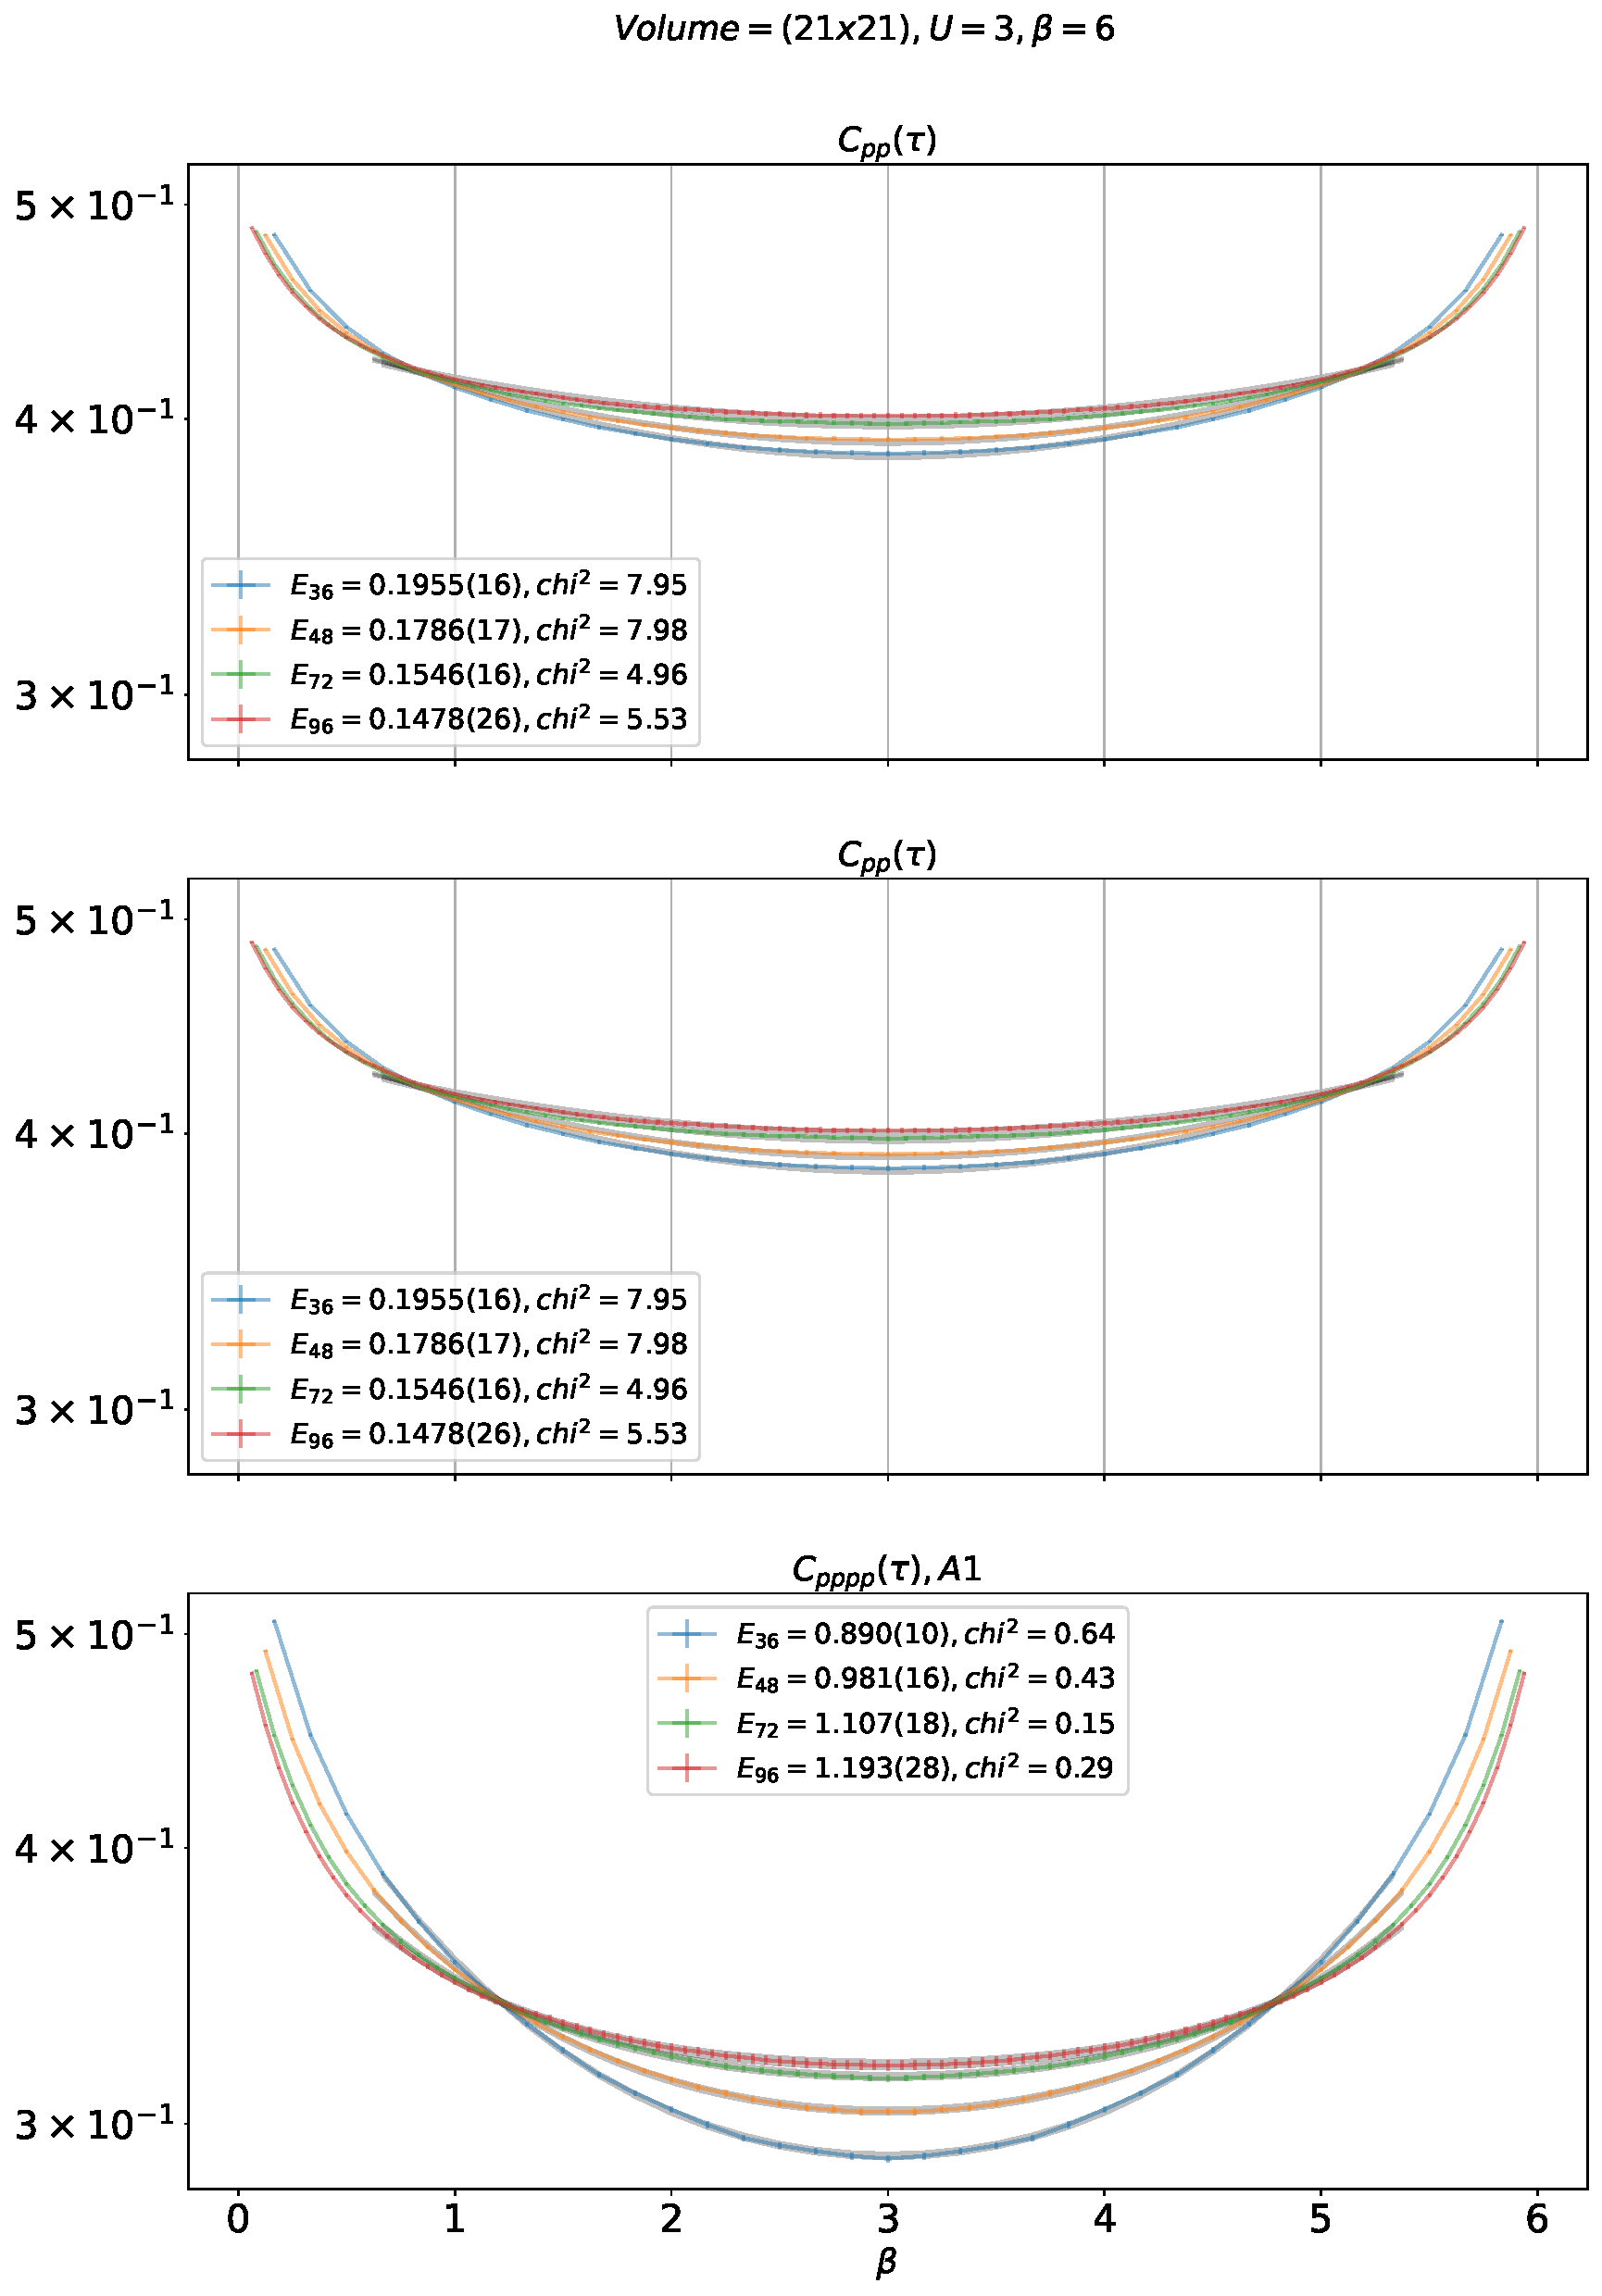
\includegraphics[width=\linewidth]{pppp-0-A1_21x21_U3_B6.pdf}
  \end{subfigure}%
  \begin{subfigure}{.5\textwidth}
    \centering
    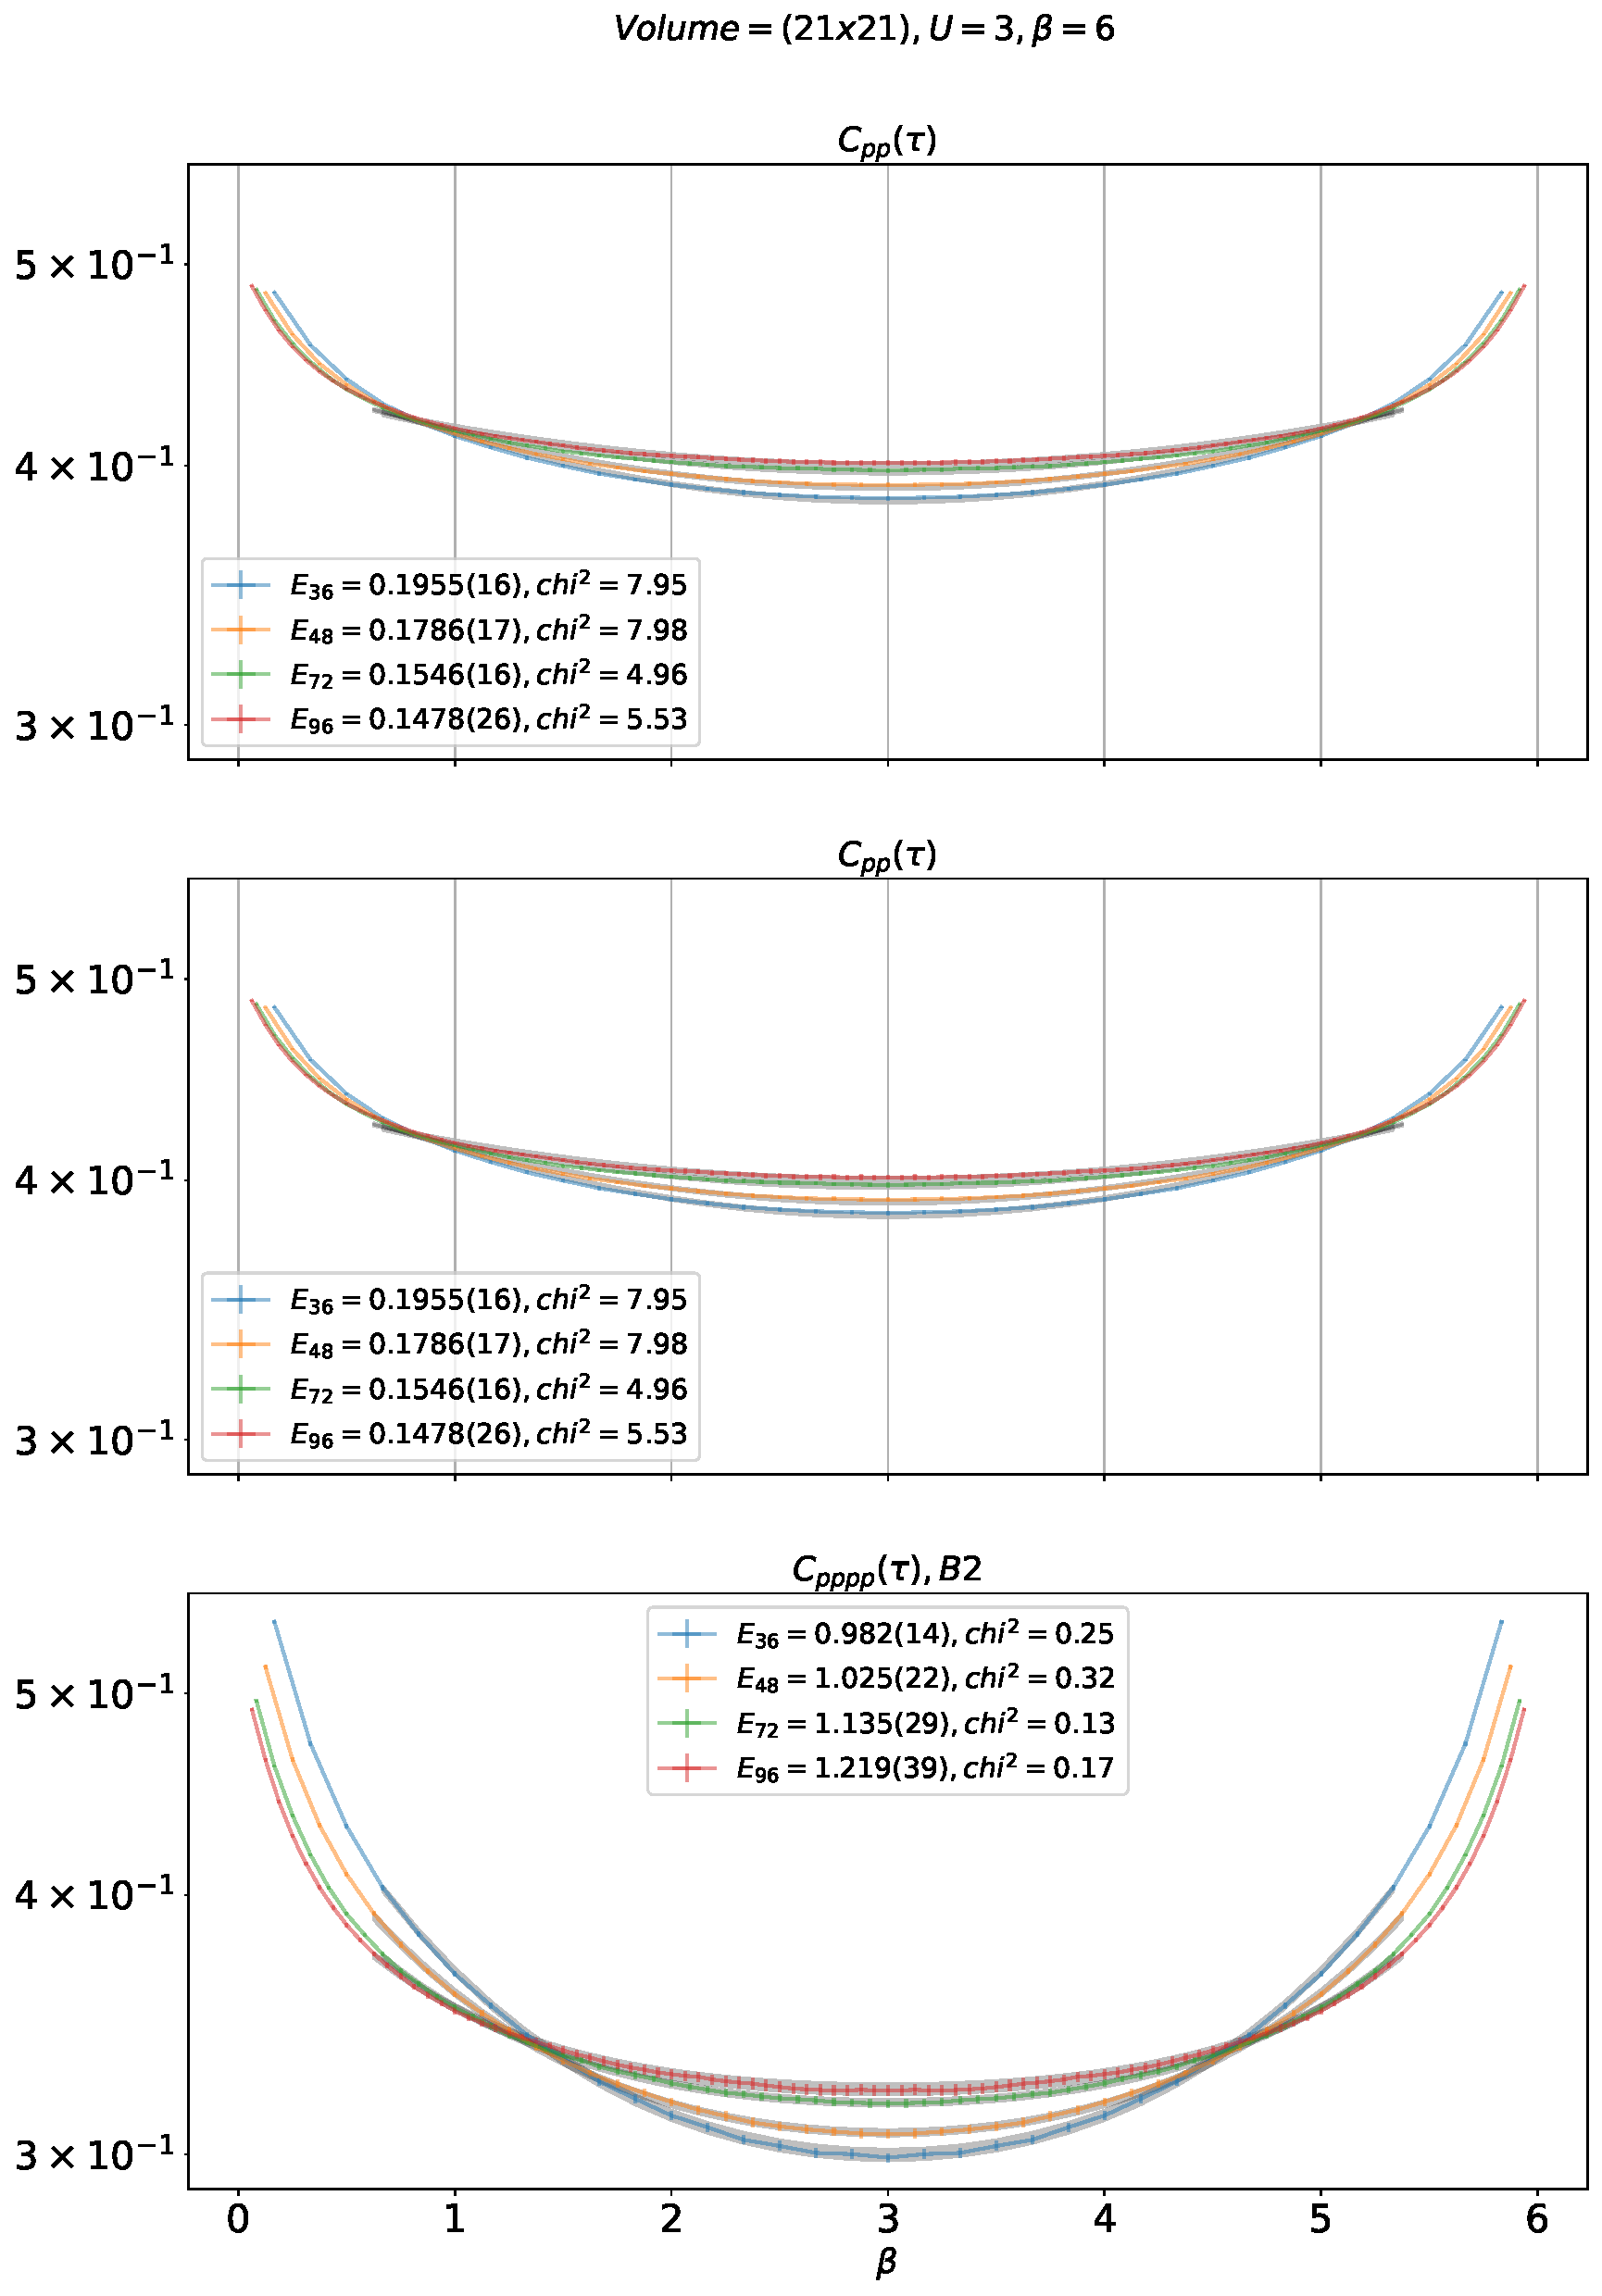
\includegraphics[width=\linewidth]{pppp-0-B2_21x21_U3_B6.pdf}
  \end{subfigure}
  \begin{subfigure}{.5\textwidth}
      \centering
      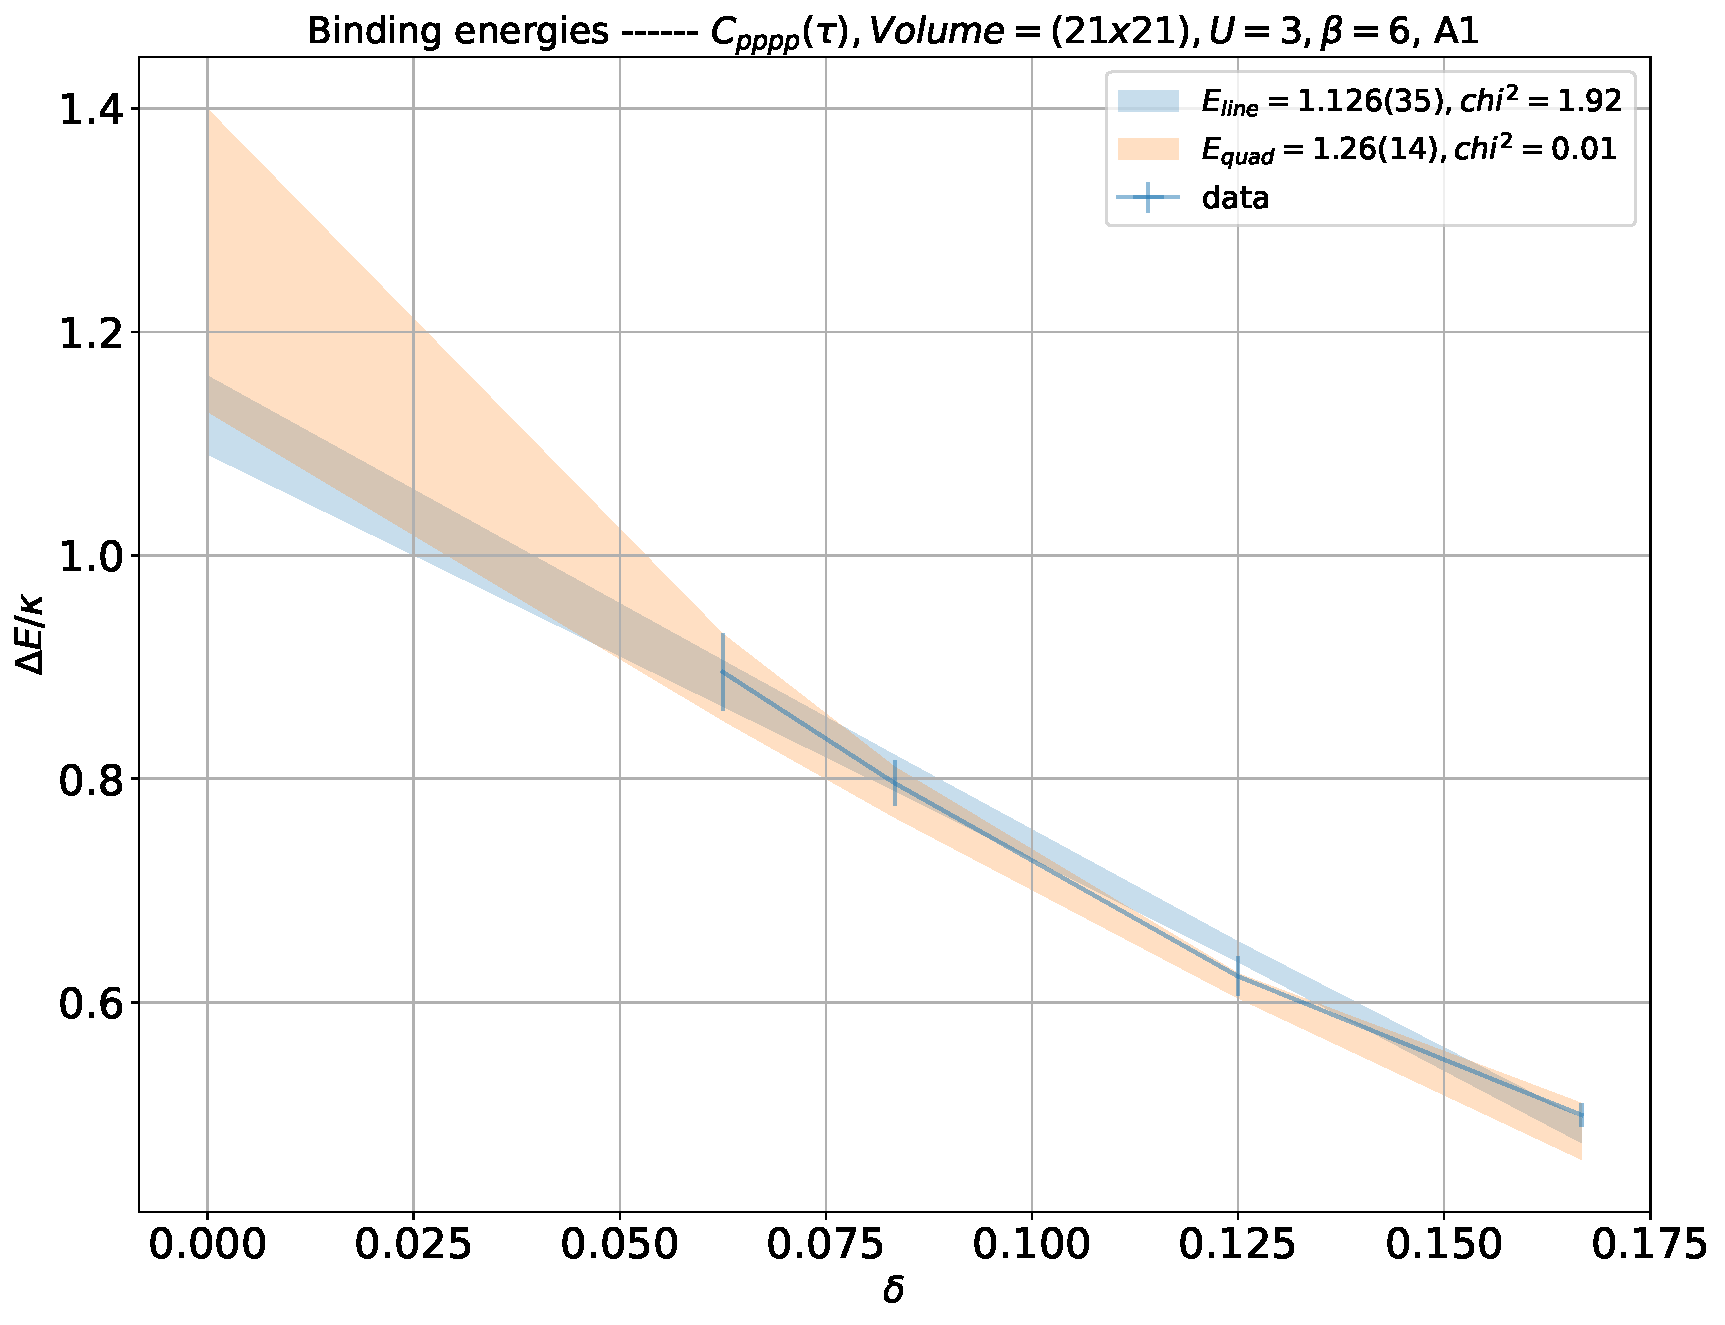
\includegraphics[width=\linewidth]{pppp-0-A1_21x21_U3_B6_cont.pdf}
  \end{subfigure}
  \begin{subfigure}{.5\textwidth}
      \centering
      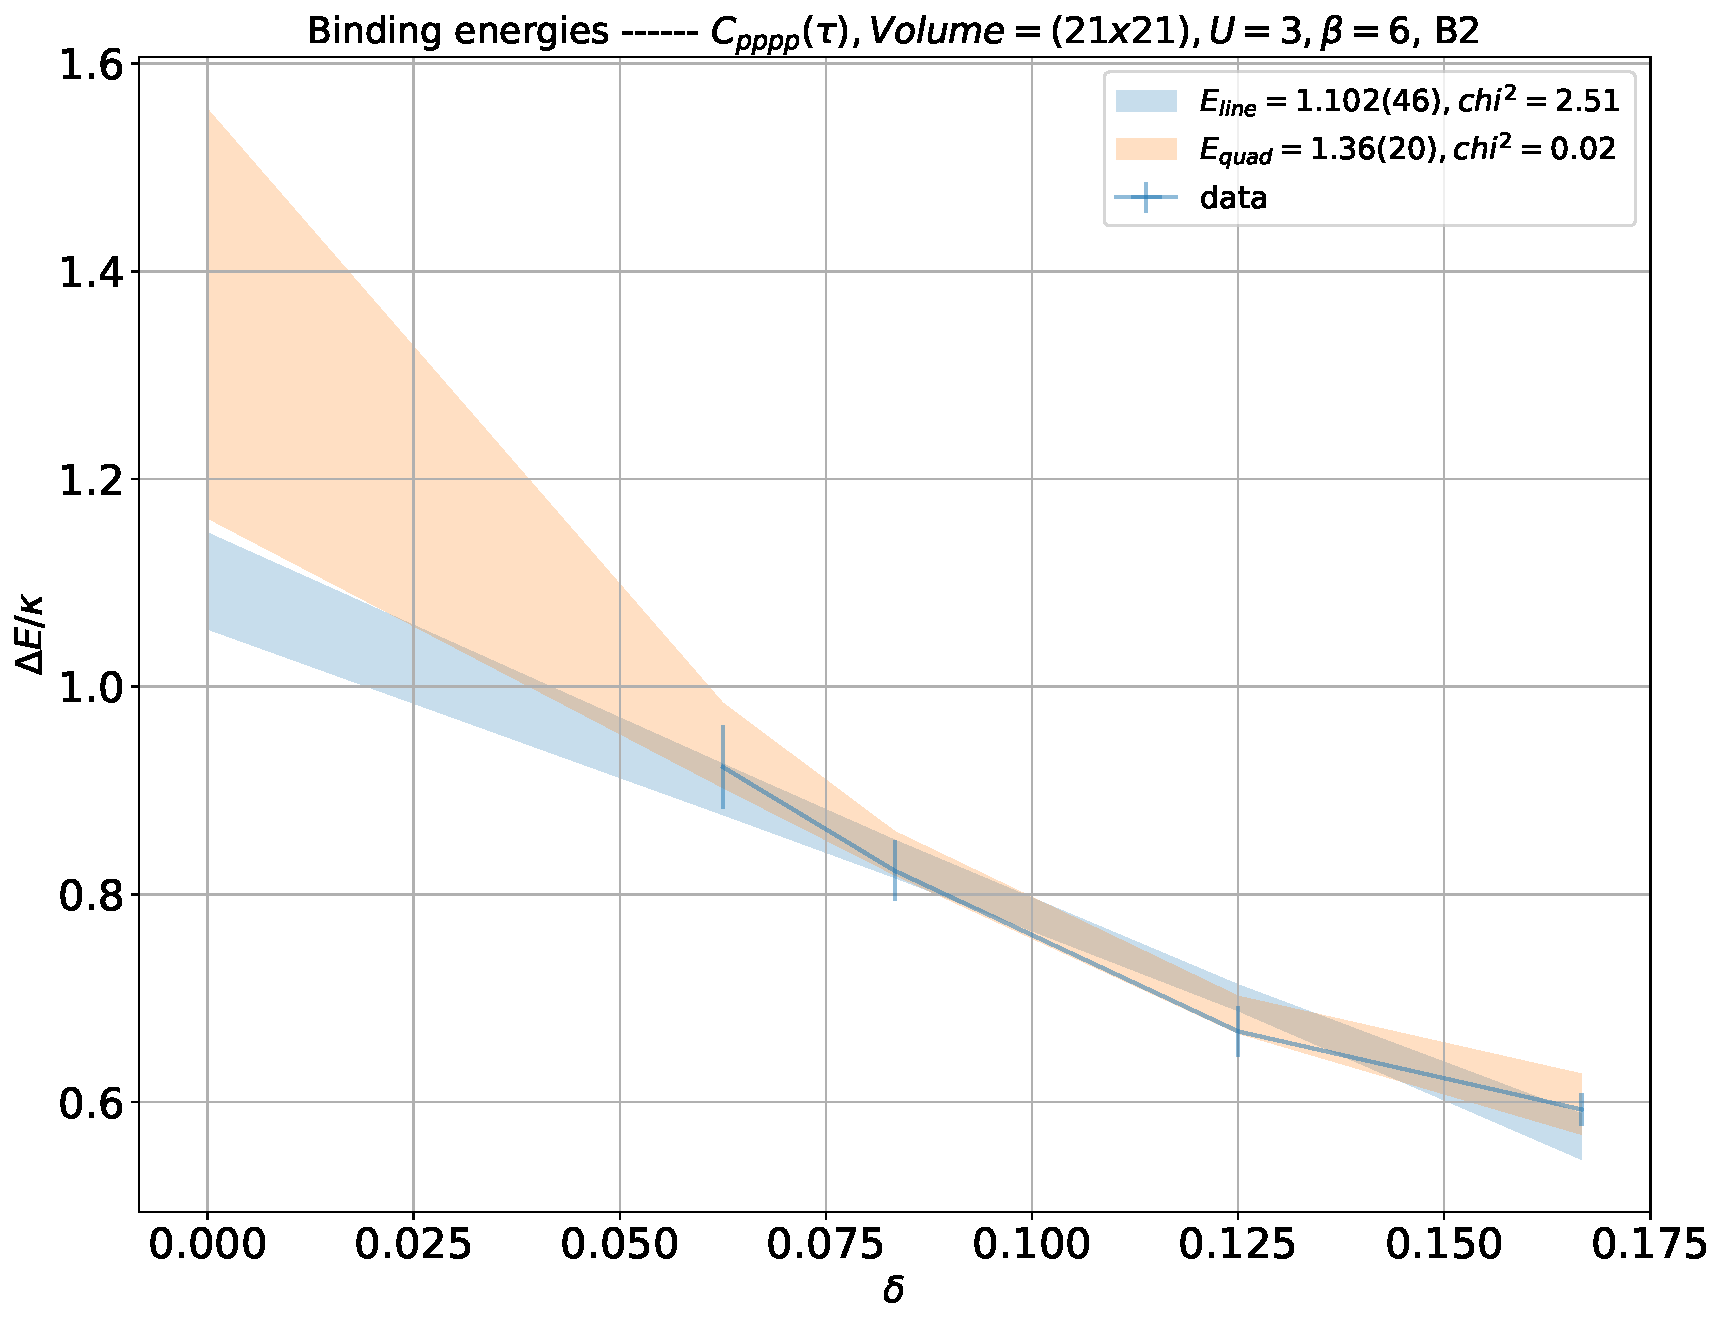
\includegraphics[width=\linewidth]{pppp-0-B2_21x21_U3_B6_cont.pdf}
  \end{subfigure}
  \caption{Binding energy extraction of the particle-particle pair at both irreducible representations, where we fit one- and two-body correlators for every $N_t$. This is followed by fitting a linear and a quadratic functions to the $\Delta E_{N_t}$ in order to extrapolate to the continuum limit ($N_t\to\infty$).}
  \label{fig:fig10}
\end{figure}
 
\begin{figure}
  \begin{subfigure}{.5\textwidth}
    \centering
    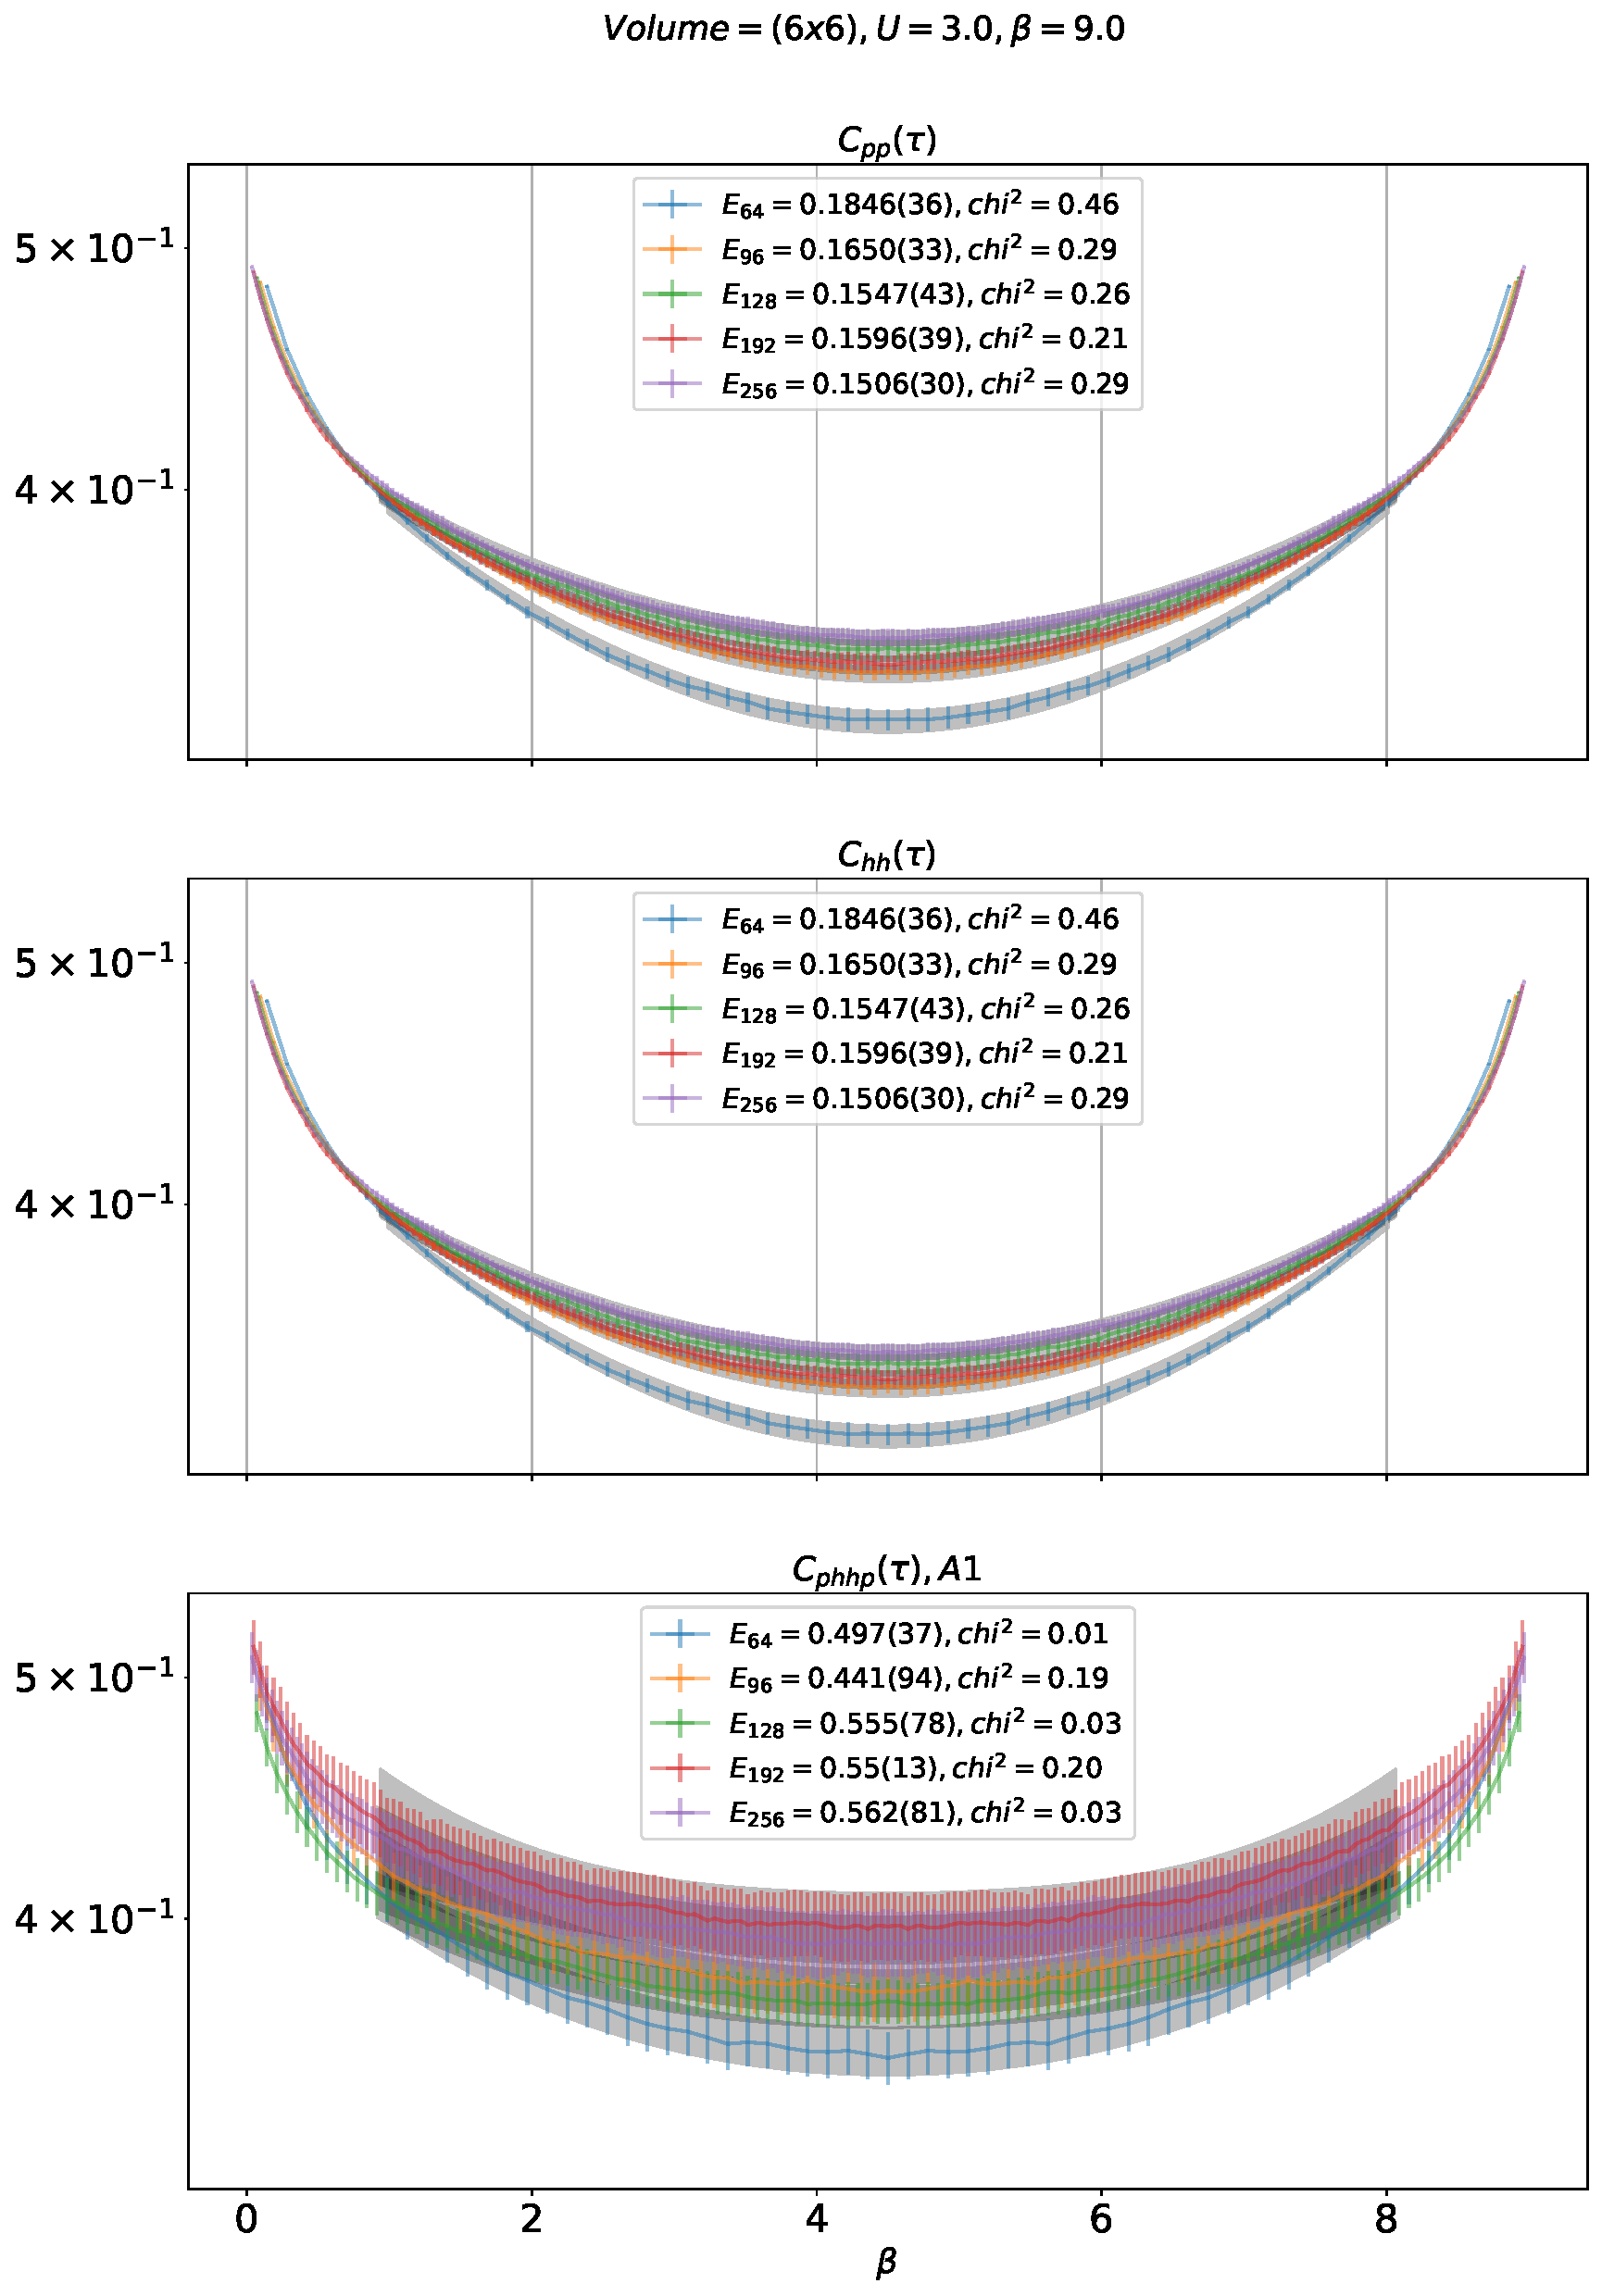
\includegraphics[width=\linewidth]{phhp-0-A1_6x6_U3.0_B9.0.pdf}
  \end{subfigure}%
  \begin{subfigure}{.5\textwidth}
    \centering
    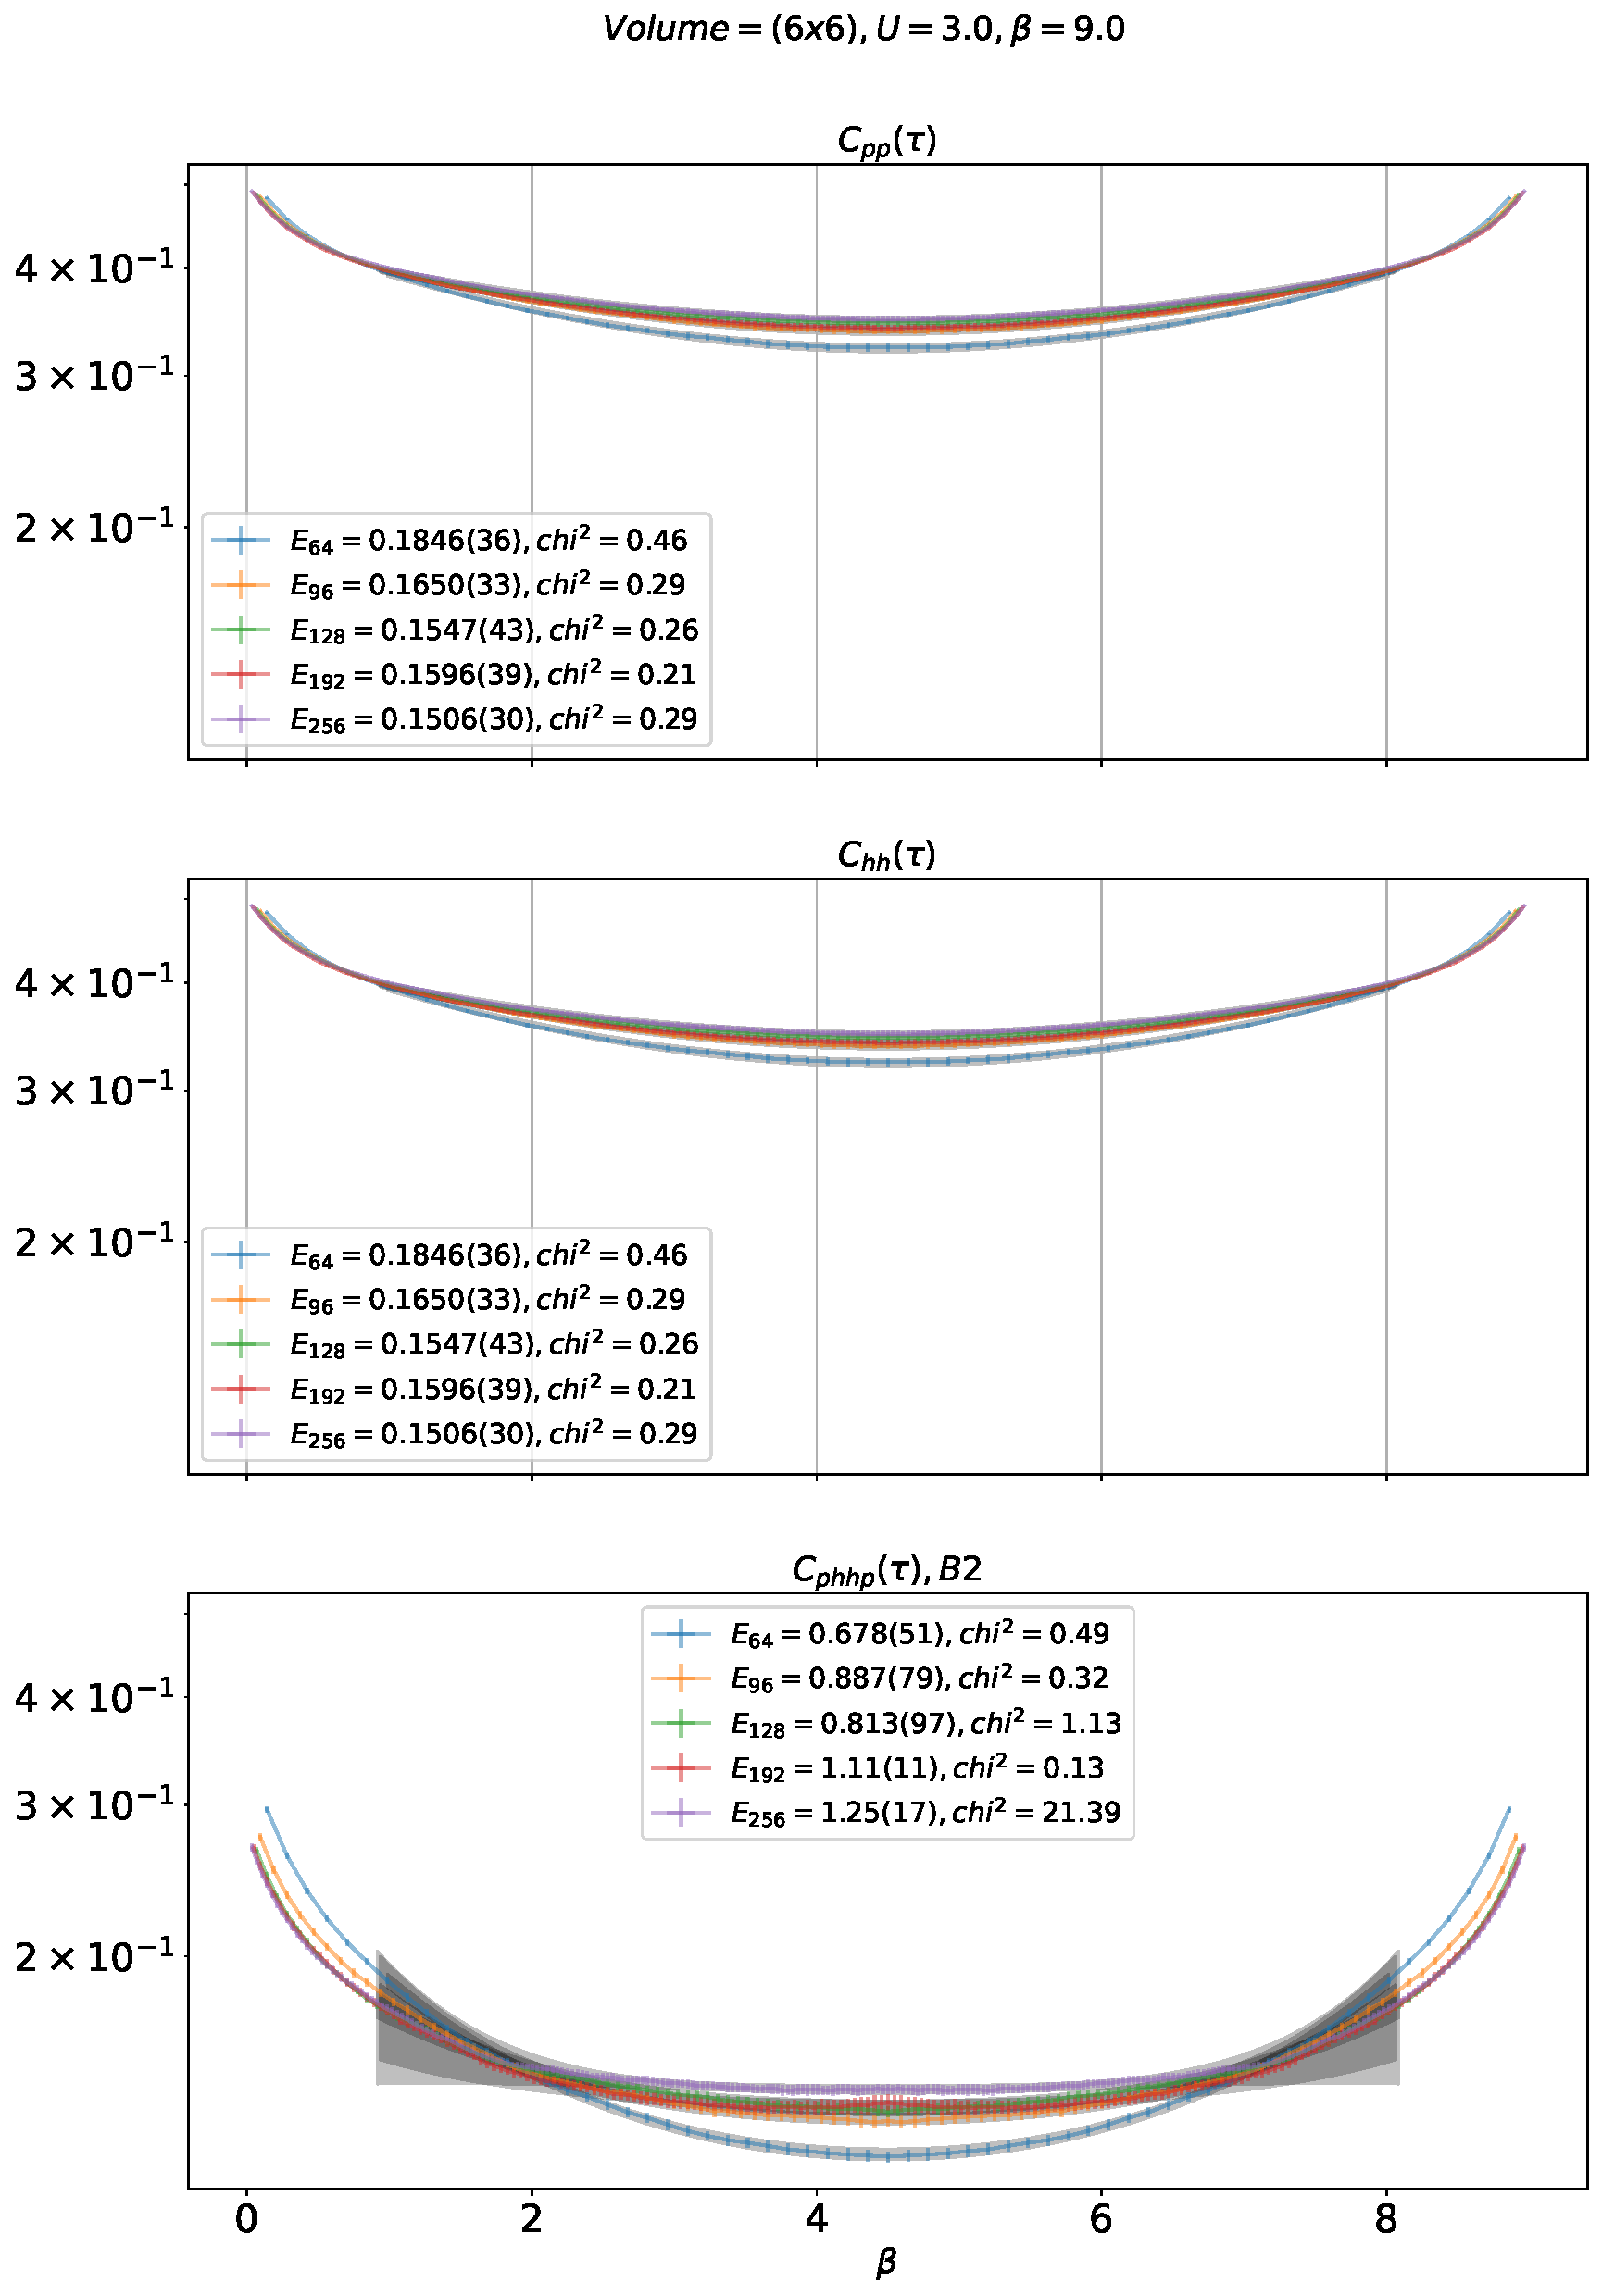
\includegraphics[width=\linewidth]{phhp-0-B2_6x6_U3.0_B9.0.pdf}
  \end{subfigure}
  \begin{subfigure}{.5\textwidth}
      \centering
      \includegraphics[width=\linewidth]{phhp-0-A1_6x6_U3.0_B9.0_cont.pdf}
  \end{subfigure}
  \begin{subfigure}{.5\textwidth}
      \centering
      \includegraphics[width=\linewidth]{phhp-0-B2_6x6_U3.0_B9.0_cont.pdf}
  \end{subfigure}
  \caption{Binding energy extraction of the particle-hole pair at both irreducible representations, where we fit one- and two-body correlators for every $N_t$. This is followed by fitting a linear and a quadratic functions to the $\Delta E_{N_t}$ in order to extrapolate to the continuum limit ($N_t\to\infty$).}
  \label{fig:fig11}
\end{figure}

\begin{figure}
  \begin{subfigure}{.5\textwidth}
    \centering
    \includegraphics[width=\linewidth]{phhp-0-A1_6x6_U3.0_B24.0.pdf}
  \end{subfigure}%
  \begin{subfigure}{.5\textwidth}
    \centering
    \includegraphics[width=\linewidth]{phhp-0-B2_6x6_U3.0_B24.0.pdf}
  \end{subfigure}
  \begin{subfigure}{.5\textwidth}
      \centering
      \includegraphics[width=\linewidth]{phhp-0-A1_6x6_U3.0_B24.0_cont.pdf}
  \end{subfigure}
  \begin{subfigure}{.5\textwidth}
      \centering
      \includegraphics[width=\linewidth]{phhp-0-B2_6x6_U3.0_B24.0_cont.pdf}
  \end{subfigure}
  \caption{Binding energy extraction of the particle-hole pair at both irreducible representations, where we fit one- and two-body correlators for every $N_t$. This is followed by fitting a linear and a quadratic functions to the $\Delta E_{N_t}$ in order to extrapolate to the continuum limit ($N_t\to\infty$).}
  \label{fig:fig12}
\end{figure}

\begin{figure}
  \begin{subfigure}{.5\textwidth}
    \centering
    \includegraphics[width=\linewidth]{pppp-0-A1_6x6_U3.0_B9.0.pdf}
  \end{subfigure}%
  \begin{subfigure}{.5\textwidth}
    \centering
    \includegraphics[width=\linewidth]{pppp-0-B2_6x6_U3.0_B9.0.pdf}
  \end{subfigure}
  \begin{subfigure}{.5\textwidth}
      \centering
      \includegraphics[width=\linewidth]{pppp-0-A1_6x6_U3.0_B9.0_cont.pdf}
  \end{subfigure}
  \begin{subfigure}{.5\textwidth}
      \centering
      \includegraphics[width=\linewidth]{pppp-0-B2_6x6_U3.0_B9.0_cont.pdf}
  \end{subfigure}
  \caption{Binding energy extraction of the particle-particle pair at both irreducible representations, where we fit one- and two-body correlators for every $N_t$. This is followed by fitting a linear and a quadratic functions to the $\Delta E_{N_t}$ in order to extrapolate to the continuum limit ($N_t\to\infty$).}
  \label{fig:fig13}
\end{figure}

\begin{figure}
  \begin{subfigure}{.5\textwidth}
    \centering
    \includegraphics[width=\linewidth]{pppp-0-A1_6x6_U3.0_B24.0.pdf}
  \end{subfigure}%
  \begin{subfigure}{.5\textwidth}
    \centering
    \includegraphics[width=\linewidth]{pppp-0-B2_6x6_U3.0_B24.0.pdf}
  \end{subfigure}
  \begin{subfigure}{.5\textwidth}
      \centering
      \includegraphics[width=\linewidth]{pppp-0-A1_6x6_U3.0_B24.0_cont.pdf}
  \end{subfigure}
  \begin{subfigure}{.5\textwidth}
      \centering
      \includegraphics[width=\linewidth]{pppp-0-B2_6x6_U3.0_B24.0_cont.pdf}
  \end{subfigure}
  \caption{Binding energy extraction of the particle-particle pair at both irreducible representations, where we fit one- and two-body correlators for every $N_t$. This is followed by fitting a linear and a quadratic functions to the $\Delta E_{N_t}$ in order to extrapolate to the continuum limit ($N_t\to\infty$).}
  \label{fig:fig14}
\end{figure}

\begin{figure}
  \begin{subfigure}{.5\textwidth}
    \centering
    \includegraphics[width=\linewidth]{phhp-0-A1_6x6_U4.0_B6.0.pdf}
  \end{subfigure}%
  \begin{subfigure}{.5\textwidth}
    \centering
    \includegraphics[width=\linewidth]{phhp-0-B2_6x6_U4.0_B6.0.pdf}
  \end{subfigure}
  \begin{subfigure}{.5\textwidth}
      \centering
      \includegraphics[width=\linewidth]{phhp-0-A1_6x6_U4.0_B6.0_cont.pdf}
  \end{subfigure}
  \begin{subfigure}{.5\textwidth}
      \centering
      \includegraphics[width=\linewidth]{phhp-0-B2_6x6_U4.0_B6.0_cont.pdf}
  \end{subfigure}
  \caption{Binding energy extraction of the particle-hole pair at both irreducible representations, where we fit one- and two-body correlators for every $N_t$. This is followed by fitting a linear and a quadratic functions to the $\Delta E_{N_t}$ in order to extrapolate to the continuum limit ($N_t\to\infty$).}
  \label{fig:fig15}
\end{figure}

\begin{figure}
  \begin{subfigure}{.5\textwidth}
    \centering
    \includegraphics[width=\linewidth]{phhp-0-A1_6x6_U4.0_B9.0.pdf}
  \end{subfigure}%
  \begin{subfigure}{.5\textwidth}
    \centering
    \includegraphics[width=\linewidth]{phhp-0-B2_6x6_U4.0_B9.0.pdf}
  \end{subfigure}
  \begin{subfigure}{.5\textwidth}
      \centering
      \includegraphics[width=\linewidth]{phhp-0-A1_6x6_U4.0_B9.0_cont.pdf}
  \end{subfigure}
  \begin{subfigure}{.5\textwidth}
      \centering
      \includegraphics[width=\linewidth]{phhp-0-B2_6x6_U4.0_B9.0_cont.pdf}
  \end{subfigure}
  \caption{Binding energy extraction of the particle-hole pair at both irreducible representations, where we fit one- and two-body correlators for every $N_t$. This is followed by fitting a linear and a quadratic functions to the $\Delta E_{N_t}$ in order to extrapolate to the continuum limit ($N_t\to\infty$).}
  \label{fig:fig16}
\end{figure}

\begin{figure}
  \begin{subfigure}{.5\textwidth}
    \centering
    \includegraphics[width=\linewidth]{phhp-0-A1_6x6_U4.0_B24.0.pdf}
  \end{subfigure}%
  \begin{subfigure}{.5\textwidth}
    \centering
    \includegraphics[width=\linewidth]{phhp-0-B2_6x6_U4.0_B24.0.pdf}
  \end{subfigure}
  \begin{subfigure}{.5\textwidth}
      \centering
      \includegraphics[width=\linewidth]{phhp-0-A1_6x6_U4.0_B24.0_cont.pdf}
  \end{subfigure}
  \begin{subfigure}{.5\textwidth}
      \centering
      \includegraphics[width=\linewidth]{phhp-0-B2_6x6_U4.0_B24.0_cont.pdf}
  \end{subfigure}
  \caption{Binding energy extraction of the particle-hole pair at both irreducible representations, where we fit one- and two-body correlators for every $N_t$. This is followed by fitting a linear and a quadratic functions to the $\Delta E_{N_t}$ in order to extrapolate to the continuum limit ($N_t\to\infty$).}
  \label{fig:fig17}
\end{figure}

\begin{figure}
  \begin{subfigure}{.5\textwidth}
    \centering
    \includegraphics[width=\linewidth]{pppp-0-A1_6x6_U4.0_B6.0.pdf}
  \end{subfigure}%
  \begin{subfigure}{.5\textwidth}
    \centering
    \includegraphics[width=\linewidth]{pppp-0-B2_6x6_U4.0_B6.0.pdf}
  \end{subfigure}
  \begin{subfigure}{.5\textwidth}
      \centering
      \includegraphics[width=\linewidth]{pppp-0-A1_6x6_U4.0_B6.0_cont.pdf}
  \end{subfigure}
  \begin{subfigure}{.5\textwidth}
      \centering
      \includegraphics[width=\linewidth]{pppp-0-B2_6x6_U4.0_B6.0_cont.pdf}
  \end{subfigure}
  \caption{Binding energy extraction of the particle-particle pair at both irreducible representations, where we fit one- and two-body correlators for every $N_t$. This is followed by fitting a linear and a quadratic functions to the $\Delta E_{N_t}$ in order to extrapolate to the continuum limit ($N_t\to\infty$).}
  \label{fig:fig18}
\end{figure}

\begin{figure}
  \begin{subfigure}{.5\textwidth}
    \centering
    \includegraphics[width=\linewidth]{pppp-0-A1_6x6_U4.0_B9.0.pdf}
  \end{subfigure}%
  \begin{subfigure}{.5\textwidth}
    \centering
    \includegraphics[width=\linewidth]{pppp-0-B2_6x6_U4.0_B9.0.pdf}
  \end{subfigure}
  \begin{subfigure}{.5\textwidth}
      \centering
      \includegraphics[width=\linewidth]{pppp-0-A1_6x6_U4.0_B9.0_cont.pdf}
  \end{subfigure}
  \begin{subfigure}{.5\textwidth}
      \centering
      \includegraphics[width=\linewidth]{pppp-0-B2_6x6_U4.0_B9.0_cont.pdf}
  \end{subfigure}
  \caption{Binding energy extraction of the particle-particle pair at both irreducible representations, where we fit one- and two-body correlators for every $N_t$. This is followed by fitting a linear and a quadratic functions to the $\Delta E_{N_t}$ in order to extrapolate to the continuum limit ($N_t\to\infty$).}
  \label{fig:fig19}
\end{figure}

\begin{figure}
  \begin{subfigure}{.5\textwidth}
    \centering
    \includegraphics[width=\linewidth]{pppp-0-A1_6x6_U4.0_B24.0.pdf}
  \end{subfigure}%
  \begin{subfigure}{.5\textwidth}
    \centering
    \includegraphics[width=\linewidth]{pppp-0-B2_6x6_U4.0_B24.0.pdf}
  \end{subfigure}
  \begin{subfigure}{.5\textwidth}
      \centering
      \includegraphics[width=\linewidth]{pppp-0-A1_6x6_U4.0_B24.0_cont.pdf}
  \end{subfigure}
  \begin{subfigure}{.5\textwidth}
      \centering
      \includegraphics[width=\linewidth]{pppp-0-B2_6x6_U4.0_B24.0_cont.pdf}
  \end{subfigure}
  \caption{Binding energy extraction of the particle-particle pair at both irreducible representations, where we fit one- and two-body correlators for every $N_t$. This is followed by fitting a linear and a quadratic functions to the $\Delta E_{N_t}$ in order to extrapolate to the continuum limit ($N_t\to\infty$).}
  \label{fig:fig20}
\end{figure}

%The \LaTeX\ WikiBook~\cite{latexwiki} is a useful source of information on \LaTeX.

% \printbibliography[heading=subbibliography]

%------------------------------------------------------------------------------
% Use biblatex for the bibliography
% Add bibliography to Table of Contents
% Comment out this command if your references are printed for each chapter.
\printbibliography[heading=bibintoc]

%------------------------------------------------------------------------------
% Declare lists of figures and tables and acknowledgements as backmatter
% Chapter/section numbers are turned off
\backmatter

\listoffigures
\listoftables

%------------------------------------------------------------------------------
% Print the glossary and list of acronyms
% \printglossaries

%------------------------------------------------------------------------------
% You could instead add your acknowledgements here - don't forget to
% also add them to \includeonly above
% %------------------------------------------------------------------------------
\chapter*{Acknowledgements}
\label{sec:ack}
%------------------------------------------------------------------------------

I would like to thank first and foremost my supervisors Prof. Dr. Stefan Krieg and Prof. Dr. Thomas Luu who introduced me into the field of Computational Physics. They gave me the incredible opportunity to work with them at Forschungszentrum Jülich on this project. 

I am extremely grateful to Dr. Evan Berkowitz, with whom I was closely working. His guidance and continuous support helped me throughout my master's thesis. I am also grateful for the excellent notes that Evan provided, which laid the groundwork for my thesis.

Special thanks to my colleagues Keshvi, Christoph, Johann, Nico, and Marcel for the ideas and suggestions in the meetings throughout the year. Especially Aleksandra Salkina who supported me throughout my whole Master's study. I also sincerely acknowledge the computing time granted through JARA on the supercomputer JURECA at Forschungszentrum Jülich.

% You should probably use \texttt{\textbackslash chapter*} for
% acknowledgements at the beginning of a thesis and
% \texttt{\textbackslash chapter} for the end.

%%% Local Variables: 
%%% mode: latex
%%% TeX-master: "../mythesis"
%%% End: 


%------------------------------------------------------------------------------
% CV needed when you submit your PhD thesis
% \definecolor{lightgray}{gray}{0.8}
\newcolumntype{L}{>{\raggedleft}p{0.15\textwidth}}
\newcolumntype{R}{p{0.8\textwidth}}
\newcommand\VRule{\color{lightgray}\vrule width 0.5pt}

\thispagestyle{empty}
\section*{Curriculum Vitae}

\subsection*{Personal Details}

\begin{tabular}{L!{\VRule}R}
Name & Johann Schmidt \\
Date of Birth &  \\
Email & abc@physik.uni-def.de \\
Family status & Single
\end{tabular}

\subsection*{Education}

\begin{tabular}{L!{\VRule}R}
1997--2003 & Abitur, ABC Secondary School, Hamburg, Germany\\
2004--2007 & BSc in Physics, Rheinische Friedrich-Wilhelms-Universität, Bonn, Germany.\\
2006 & CERN Summer Student, Geneva, Switzerland. \\
2007--2009 &  MSc in Physics Rheinische Friedrich-Wilhelms-Universität, Bonn, Germany. \\
2009--2012 &  PhD in Physics, Rheinische Friedrich-Wilhelms-Universität, Bonn, Germany. \\
2012 & Advanced Data Analysis School, Frankfurt, Germany.
\end{tabular}

\subsection*{Professional Experience}

\begin{tabular}{L!{\VRule}R}
2004 & Summer Student at CERN, Geneva, Switzerland. \\
2007--2012 & Doctoral work at the University of Bonn, Germany. \\
2008--2009 & Fieldwork at CERN, Geneva, Switzerland.\\
2011 & Talk at the Advanced Physics Conference, Timbucto
\end{tabular}

\subsection*{Languages}
\begin{tabular}{L!{\VRule}R}
German & Mother tongue \\
English & Fluent \\
Russian & Basic
\end{tabular}


\end{document}
